% \documentclass[imslayout,preprint]{imsart} 
%\def\journal@name{} 
\documentclass[12pt]{report}
\usepackage[linenumbers,preprint]{imsart}

%\let\document\latexdocument
%\let\enddocument\latexenddocument
%%\AtEndDocument{\printhistory}
%\let\arabic\latexarabic
%\def\rm{}
\usepackage[margin=1in]{geometry}
\usepackage{amsmath}
\usepackage{amssymb,amsthm,mathtools}
\usepackage{mathtools}
\usepackage{bm}
\usepackage[unicode,colorlinks,citecolor=blue,urlcolor=black,linkcolor=blue,pdfborder={0 0 0}]{hyperref}
\usepackage[capitalize,sort,compress]{cleveref} % nice reference package for automatically choosing names for references
\usepackage{comment}
\usepackage{graphicx}
\usepackage{enumitem}
\usepackage{framed}
\usepackage{dcolumn}
%%% UNCOMMENT WHEN SUBMITTING TO ARXIV %%%
\usepackage{chngcntr}
%\usepackage{subcaption}
\usepackage{dsfont} % doublestroke fonts (for things like reals, nats, complex numbers, etc)


\usepackage{url} % nice URL typesetting
\usepackage[usenames]{color} % for using colored text
\usepackage{subfig}
\usepackage[sort]{natbib}
%\usepackage[style=numeric-comp,
%       minnames=1,
%       maxnames=99,
%       maxcitenames=3,
%       natbib=true,
%       firstinits=true,
%       backend=bibtex]{biblatex}

\usepackage{datetime}
\usepackage[normalem]{ulem}
\usepackage[linesnumbered,ruled,vlined]{algorithm2e}

\usepackage{autonum}
\usepackage{microtype} % microtypesetting improvements for latex
\usepackage{booktabs} % professional quality tables
\usepackage{graphicx}
\usepackage{thmtools}

\usepackage{tikz}
\usepackage{pgfplots}

\newtheorem{assumption}{Assumption}
\newtheorem{theorem}{Theorem}
\newtheorem{proposition}{Proposition}
\newtheorem{lemma}{Lemma}
\newtheorem{example}{Example}
\newtheorem{definition}{Definition}
\newtheorem{remark}{Remark}
\newenvironment{contexample}{
   \addtocounter{example}{-1} \begin{example}[continued]}{
   \end{example}}

\crefname{theorem}{Theorem}{Theorems}
\crefname{lemma}{Lemma}{Lemmas}
\crefname{proposition}{Proposition}{Propositions}
\crefname{corollary}{Corollary}{Corollaries}
\crefname{conjecture}{Conjecture}{Conjectures}
\crefname{definition}{Definition}{Definitions}
\crefname{assumption}{Assumption}{Assumptions}
\crefname{example}{Example}{Examples}
\crefname{remark}{Remark}{Remarks}
\crefname{algocf}{Algorithm}{Algorithms}


\renewcommand{\textfraction}{0.1}
\renewcommand{\floatpagefraction}{0.9}
\captionsetup[figure]{font=small,labelfont=small}

\AtBeginDocument{ %necessary to stop clash with autonum package
\def\[#1\]{\begin{align}#1\end{align}}
}

\newcommand{\methodname}{\textsf{ACDC}\xspace}

%%%%%%%%%%%%%%%%%%
%%% Commenting %%% 
%%%%%%%%%%%%%%%%%%

%% NA: needs attention (rough writing whose correctness needs to be verified)
%% TBD: instructions for how to fix a gap ("Describe the propagation by ...")
%% PROBLEM: bug or missing crucial bit 

%% use \fXXX versions of these macros to put additional explanation into a footnote (in the margin).  
%% The idea is that we don't want to interrupt the flow of the paper or make it 
%% impossible to read because there are a bunch of comments.

%% NA's (and TBDs, those less crucially) should be written so 
%% that they flow with the text.

\definecolor{WowColor}{rgb}{.75,0,.75}
\definecolor{SubtleColor}{rgb}{0,0,.50}

% inline
\newcommand{\NA}[1]{\textcolor{SubtleColor}{ {\tiny \bf ($\star$)} #1}}
\newcommand{\LATER}[1]{\textcolor{SubtleColor}{ {\tiny \bf ($\dagger$)} #1}}
\newcommand{\TBD}[1]{\textcolor{SubtleColor}{ {\tiny \bf (!)} #1}}
\newcommand{\PROBLEM}[1]{\textcolor{WowColor}{ {\bf (!!)} {\bf #1}}}

% as margin notes
\newcounter{margincounter}
\newcommand{\displaycounter}{{\arabic{margincounter}}}
\newcommand{\incdisplaycounter}{{\stepcounter{margincounter}\arabic{margincounter}}}

\newcommand{\fTBD}[1]{\textcolor{SubtleColor}{$\,^{(\incdisplaycounter)}$}\marginpar{\tiny\textcolor{SubtleColor}{ {\tiny $(\displaycounter)$} #1}}}

\newcommand{\fPROBLEM}[1]{\textcolor{WowColor}{$\,^{((\incdisplaycounter))}$}\marginpar{\tiny\textcolor{WowColor}{ {\bf $\mathbf{((\displaycounter))}$} {\bf #1}}}}

\newcommand{\fLATER}[1]{\textcolor{SubtleColor}{$\,^{(\incdisplaycounter\dagger)}$}\marginpar{\tiny\textcolor{SubtleColor}{ {\tiny $(\displaycounter\dagger)$} #1}}}

\DeclareRobustCommand{\suppresscomments}{
	% For submission, make all render blank.
	\renewcommand{\LATER}[1]{}
	\renewcommand{\fLATER}[1]{}
	\renewcommand{\TBD}[1]{}
	\renewcommand{\fTBD}[1]{}
	\renewcommand{\PROBLEM}[1]{}
	\renewcommand{\fPROBLEM}[1]{}
	\renewcommand{\NA}[1]{##1}  %% Note, NA's pass through!
}


\newcommand{\charalphabetmacro}[3]{
	% #1: annotation prefix
	% #2: annotation command (must be a single command!)
	% #3: characters to define annotations for
	% Create a macros of the form
	%   \newcommand{\#1##1}{#2{##1}} for each ##1 in #3
	\def\mydeffoo##1{\expandafter\def\csname #1##1\endcsname{#2{##1}}}
	\def\mydefallfoo##1{\ifx##1\mydefallfoo\else\mydeffoo##1\expandafter\mydefallfoo\fi}
	\expandafter \mydefallfoo #3\mydefallfoo
}

\newcommand{\texalphabetmacro}[3]{
	% #1: annotation prefix
	% #2: annotation command (must be a single command!)
	% #3: latex symbol command text to define annotations for
	% Create a macros of the form
	%   \newcommand{\#1##1}{#2{\##1}} for each ##1 in #3
	\def\mydeftex##1{\expandafter\def\csname #1##1\endcsname{#2{\csname ##1\endcsname}}}
	\def\mydefalltex##1{\ifx\mydefalltex##1\else\mydeftex{##1}%
			\lowercase{\mydeftex{##1}}\expandafter\mydefalltex\fi}
	\expandafter \mydefalltex #3\mydefalltex
}

\newcommand{\upperCaseRomanLetters}{ABCDEFGHIJKLMNOPQRSTUVWXYZ}
\newcommand{\lowerCaseRomanLetters}{abcdefghijklmnopqrstuvwxyz}
\newcommand{\lowerCaseRomanLettersNoMHT}{abcdefgijklnopqrsuvwxyz}
\newcommand{\lowerCaseRomanLettersNoG}{abcdefhijklmnopqrstuvwxyz}
\newcommand{\lowerCaseRomanLettersNoMF}{abcdeghijklnopqrstuvwxyz}


\newcommand{\lowerCaseGreekLetters}{{alpha}{beta}{gamma}{delta}{epsilon}{zeta}{eta}{theta}{iota}{kappa}{lambda}{mu}{nu}{xi}{omicron}{pi}{rho}{sigma}{tau}{upsilon}{phi}{chi}{psi}{omega}}
\newcommand{\lowerCaseGreekLettersNoEta}{{alpha}{beta}{gamma}{delta}{epsilon}{zeta}{theta}{iota}{kappa}{lambda}{mu}{nu}{xi}{omicron}{pi}{rho}{sigma}{tau}{upsilon}{phi}{chi}{psi}{omega}}
\newcommand{\upperCaseGreekLettersInLaTeX}{{Gamma}{Delta}{Theta}{Lambda}{Xi}{Pi}{Sigma}{Upsilon}{Phi}{Psi}{Omega}}


% Bar everything shortcuts
\charalphabetmacro{bar}{\bar}{\upperCaseRomanLetters}
\charalphabetmacro{bar}{\bar}{\lowerCaseRomanLetters}

\charalphabetmacro{b}{\boldorbar}{\upperCaseRomanLetters}
\charalphabetmacro{b}{\boldorbar}{\lowerCaseRomanLettersNoMF} % avoid clash with \bm and \bf
\newcommand{\boldf}{\bm{f}} % only need \boldf, since \barf already defined above

\texalphabetmacro{b}{\boldorbar}{\lowerCaseGreekLettersNoEta} % avoid \beta <-> \bar{\eta} clash
\newcommand{\bareta}{\bar{\eta}}
\newcommand{\boldeta}{\bm{\eta}}
\texalphabetmacro{b}{\boldorbar}{\upperCaseGreekLettersInLaTeX}

% Mathcal shortcuts
\charalphabetmacro{mc}{\mathcal}{\upperCaseRomanLetters}

\newcommand{\widehatmathcal}[1]{\widehat{\mathcal{#1}}}
\charalphabetmacro{hmc}{\widehatmathcal}{\upperCaseRomanLetters}

% Hatted shortcuts
\charalphabetmacro{h}{\widehat}{\upperCaseRomanLetters}
\charalphabetmacro{h}{\widehat}{\lowerCaseRomanLettersNoMHT}
\texalphabetmacro{h}{\widehat}{\lowerCaseGreekLetters}
\texalphabetmacro{h}{\widehat}{\upperCaseGreekLettersInLaTeX}

% Bold hatted shortcuts
\newcommand{\boldhat}[1]{\mathbf{\widehat{#1}}}
\charalphabetmacro{bh}{\boldhat}{\upperCaseRomanLetters}
\charalphabetmacro{bh}{\boldhat}{\lowerCaseRomanLetters}
\texalphabetmacro{bh}{\boldhat}{\lowerCaseGreekLetters}
\texalphabetmacro{bh}{\boldhat}{\upperCaseGreekLettersInLaTeX}


%Wide hatted shortcuts
\charalphabetmacro{wh}{\widehat}{\upperCaseRomanLetters}
\charalphabetmacro{wh}{\widehat}{\lowerCaseRomanLettersNoMHT}

% Tilde shortcuts 
\charalphabetmacro{td}{\tilde}{\upperCaseRomanLetters}
\charalphabetmacro{td}{\tilde}{\lowerCaseRomanLetters}
\texalphabetmacro{td}{\tilde}{\lowerCaseGreekLetters}
\texalphabetmacro{td}{\tilde}{\upperCaseGreekLettersInLaTeX}


\newcommand{\defas}{:=}

% Stacked Relations
%%%%%%%%%%%%%%%%%%%
\newcommand{\stk}[2]{\ensuremath{\stackrel{\text{#2}}{#1}}}
\newcommand{\stkm}[2]{\ensuremath{\stackrel{#2}{#1}}}


\newcommand{\abscont}{\ll}  % absolutely continuous 
\newcommand{\nnreals}{\reals_{+}}
\newcommand{\cconj}[1]{\overline{#1}}  % complex conjugation 
\newcommand{\im}{\operatorname{im}}

\newcommand{\fracexp}[3]{\left(\frac{#1}{#2}\right)^{#3}}
\newcommand{\gammafrac}[2]{\frac{\Gamma(#1)}{\Gamma(#2)}}
\newcommand{\textder}[2]{\dee #1/\dee #2}

\newcommand{\distSS}{\distNamed{SS}} % symmetric stable distribution 
\newcommand{\ii}{i} % imaginary unit 
\newcommand{\erfc}{\operatorname{erfc}}
\newcommand{\logit}{\psi}
\newcommand{\logistic}{\phi}
\newcommand{\derivop}[1]{\grad^{#1}}
\newcommand{\hessian}{\derivop{2}}
\newcommand{\mean}[1]{\bar#1}
\newcommand{\indicatorfn}{\mathds{1}}
\newcommand{\id}{\operatorname{id}}

\newtheorem*{notation}{Notation}
\newcommand{\littleo}{o}
\newcommand{\littleoP}{\littleo_{P}}
\newcommand{\littleoPouter}{\littleo_{P^{+}}}
\newcommand{\bigo}{O}
\newcommand{\bigoP}{\bigo_{P}}
\newcommand{\bigoPouter}{\bigo_{P^{+}}}
\newcommand{\convto}{\overset{\Pr_{\trueparam}}{\rightarrow}}
\newcommand{\convtodist}{\overset{d}{\rightarrow}}
\newcommand{\empvar}[1]{\widehat\sigma^{2}(#1)}
% \newcommand{\empcov}[1]{\widehat\Sigma(#1)}
\newcommand{\empcov}{\widehat\Sigma}
\newcommand{\empmean}[1]{\widehat\mu(#1)}

\newcommand{\statistic}[1]{T_{#1}}
\newcommand{\p}{p}


%--------------------------------------------------------------------------------------
% Sets
%--------------------------------------------------------------------------------------
\newcommand{\intersection}{\cap}

%--------------------------------------------------------------------------------------
% Bayesian stuff
%--------------------------------------------------------------------------------------


\newcommand{\model}[1]{\mcM^{(#1)}}
\newcommand{\paramSpace}[1]{\Theta^{(#1)}}

% Data
\newcommand{\truesym}{\circ}
\newcommand{\dataspace}{\mcX}
\newcommand{\obsspace}{\mathbb X}


\newcommand{\datarv}{\mathbf{X}}
\newcommand{\dataarg}[1]{x_{1:#1}}
\newcommand{\datarvarg}[1]{X_{1:#1}}
\newcommand{\datapart}[1]{\dataarg{(#1)}}
\newcommand{\alldata}{\dataarg{\infty}}
\newcommand{\alldatarv}{\datarvarg{\infty}}
\newcommand{\datacopy}{Y}
\newcommand{\datarvcopy}{\mathbf Y}
\newcommand{\datatrue}{\data_{\truesym}}
\newcommand{\obs}[1]{x_{#1}}
\newcommand{\obsrv}[1]{X_{#1}}
\newcommand{\datameanarg}[1]{\bar\data_{#1}}
\newcommand{\datarvmeanarg}[1]{\bar\datarv_{#1}}
% \newcommand{\datameanarg}[1]{\empmean{\dataarg{#1}}}


% Posterior and priors
\newcommand{\basedist}{\lambda}
\newcommand{\postdist}[1]{\Pi_{#1}}
\newcommand{\postdistfull}[2]{\Pi(#1 \given #2)}
\newcommand{\ppostdist}[2]{\Pi_{#1}^{#2}}
\newcommand{\postdensity}[1]{\pi_{#1}}
\newcommand{\postdensityfull}[2]{\pi(#1 \given #2)}
\newcommand{\ppostdensity}[2]{\pi_{#1}^{#2}}
\newcommand{\priordist}{\postdist{0}}
\newcommand{\priordensity}{\postdensity{0}}



%\newcommand{\lik}[2]{f(#1 \given #2)}
%\newcommand{\loglik}[2]{\mcL(#1 \given #2)}
%\newcommand{\Eloglik}[1]{\bar\mscL(#1)}
% log-likelihood
\newcommand{\likdist}[1]{P_{#1}}
\newcommand{\likfun}[1]{p_{#1}}
\newcommand{\lik}[2]{\likfun{#2}(#1)}
\newcommand{\loglik}[2]{\ell_{#2}(#1)}
\newcommand{\loglikfun}[1]{\ell_{#1}}
\newcommand{\Eloglik}[1]{\bar\ell_{#1}}
\newcommand{\optEloglik}{\bar\ell_{\optsym}}
\newcommand{\Eloglikdiff}[1]{\Delta_{#1}}
\newcommand{\gradloglik}[2]{\dot\ell_{#2}(#1)}
\newcommand{\gradloglikfun}[1]{\dot\ell_{#1}}
\newcommand{\hessloglik}[2]{\ddot\ell_{#2}(#1)}
\newcommand{\hessloglikfun}[1]{\ddot\ell_{#1}}

% data distributions 
\newcommand{\priormarginal}{m_\textrm{prior}}
\newcommand{\postmarginal}{m_\textrm{post}}
%\newcommand{\marginallik}[1]{p_{#1}}
%\newcommand{\pmarginallik}[2]{p(#1)^{#2}}

% parameter
\newcommand{\opt}{\star}
\newcommand{\optsym}{\star}

%
%\newcommand{\paramsample}{\vartheta}
%\newcommand{\bbparam}{\param^{\bbsym}}
%\newcommand{\bbparamsample}{\paramsample^{\bbsym}}
%\newcommand{\bbparamsamplecopy}{\paramsample^{\bbsym\prime}}
%\newcommand{\bbparamsamplenum}{\paramsample^{\bbsym}_{\numobs}}
%\newcommand{\optparams}{\paramspace_{o}}
%\newcommand{\mle}[1]{\widehat\param}
%
%% Model selection
%\newcommand{\modelspace}{\mathfrak{M}}
%\newcommand{\model}{\mathfrak{m}}
%\newcommand{\optmodel}{\model_{\optsym}}
%\newcommand{\modelmarginallik}[2]{\marginallikfull{#1 \given #2}}
%\newcommand{\modelpriordist}{Q_{0}}
%% \newcommand{\modelpostdist}[1]{Q_{#1}}
%\newcommand{\modelpostdistfull}[2]{Q(#1 \given #2)}
%\newcommand{\priorlogodds}{\rho}
%\newcommand{\lmldiff}[1]{\Lambda_{#1}}
%\newcommand{\optmodelparam}[1]{\param_{#1 \optsym}}
%
%% Fisher information
%\newcommand{\Ehessloglik}[1]{J_{#1}}
%\newcommand{\Vargradloglik}[1]{I_{#1}}
%
%\newcommand{\paramcovmat}{C}
%\newcommand{\paramcov}[2]{\paramcovmat_{#1#2}}
%
%
%\newcommand{\credset}[2]{C_{#1}(#2)}
%\newcommand{\credsetintersect}[3]{I_{#1}(#2, #3)}
%\newcommand{\normalcredsetconst}[1]{c_{#1}}
%
%% data distributions 
\newcommand{\datadist}{P_{o}}
\newcommand{\distDisc}{\mcD_{\mathrm{dist}}}
\newcommand{\compDisc}{\mcD_{\mathrm{comp}}}
\newcommand{\compDiscEst}{\widehat{\mcD}_{\mathrm{comp}}}
%\newcommand{\obsdist}{P_{\truesym}}
%\newcommand{\empdist}{\Pr_{\numobs}}
%\newcommand{\datasum}{Z}
%\newcommand{\datadiff}{W}
%
%
%% BayesBag
%\newcommand{\bbsym}{*} % BayesBag symbol
%\newcommand{\bsnumobs}{M}
%\newcommand{\bbEE}{\EE^{\bbsym}} % expectation wrt to BayesBag
%\newcommand{\bsindrvsym}{L}
%\newcommand{\bsindsym}{\ell}
%\newcommand{\bsind}[1]{\bsindsym_{#1}}
%\newcommand{\bsindrv}[1]{\bsindrvsym_{#1}}
%\newcommand{\bsindrvs}[1]{\bsindrvsym_{1:#1}}
%\newcommand{\bscount}[1]{K_{#1}}
%\newcommand{\bscounts}{K_{1:\numobs}}
%\newcommand{\bsobs}[1]{\obs{#1}^{\bbsym}}
%\newcommand{\bsobsrv}[1]{\obsrv{#1}^{\bbsym}}
%\newcommand{\bsdata}{\data^{\bbsym}}
%\newcommand{\bsdatarv}{\datarv^{\bbsym}}
%\newcommand{\bsdatasample}[1]{\data^{\bbsym}_{(#1)}}
%\newcommand{\bsdataarg}[1]{\bsdata_{1:#1}}
%\newcommand{\bsdatarvarg}[1]{\bsdatarv_{1:#1}}
%\newcommand{\bsdatacopy}[1]{\datacopy^{\bbsym}_{1:#1}}
%\newcommand{\bbpostdist}[1]{\postdist{#1}^{\bbsym}}
%\newcommand{\bbpostdistfull}[2]{\Pi^{\bbsym}(#1 \given #2)}
%\newcommand{\bbpostdensity}[1]{\postdensity{#1}^{\bbsym}}
%\newcommand{\bbpostdensityfull}[2]{\postdensity{}^{\bbsym}(#1 \given #2)}
%\newcommand{\bsdatameanarg}[1]{\bar\data^{\bbsym}_{#1}}
%\newcommand{\bsdatarvmeanarg}[1]{\bar\datarv^{\bbsym}_{#1}}
%% \newcommand{\bsdatameanarg}[1]{\empmean{\bsdataarg{#1}}}
%% \newcommand{\bsdatarvmeanarg}[1]{\empmean{\bsdatarvarg{#1}}}
%%\newcommand{\bsdatameanargrv}[1]{\bar\data_{\bsindrvsym}}
%\newcommand{\bbempdist}{\Pr_{\numobs}^{\bbsym}}
%% \newcommand{\bbmodelpostdist}[1]{Q_{#1}^{\bbsym}}
%\newcommand{\bbmodelpostdistfull}[2]{Q^{\bbsym}(#1 \given #2)}
%%\newcommand{\indexvar}[1]{\bsindrvsym_{#1}}
%
%
%\newcommand{\bsscale}{c}
%%\newcommand{\optscale}{\bsscale_{\text{opt}}}
%%\newcommand{\optscaleest}{\widehat\bsscale_{\text{opt}}}
%\newcommand{\optMasympt}{\bsnumobs_{\infty,\text{opt}}}
%\newcommand{\optMasymptest}{\widehat\bsnumobs_{\infty,\text{opt}}}
%\newcommand{\optMfs}{\bsnumobs_{\text{fs,opt}}}
%\newcommand{\optMfsest}{\widehat\bsnumobs_{\text{fs,opt}}}
%\newcommand{\optMest}{\widehat\bsnumobs_{\text{opt}}}
%\newcommand{\modelmismatch}{\mathcal{I}}
%\newcommand{\nan}{\textsf{NA}}
%\newcommand{\concconst}{C_{\numobs}}
%
%% Split Predictive Checks
%
%
%\newcommand{\pcobsrv}{X_{\text{obs}}}    % X
%\newcommand{\pcobsobs}[1]{\obsrv{#1}}
%\newcommand{\pcnewrv}{X_{\text{ho}}}  % X^rep
%\newcommand{\pcreprv}{X_{\text{pred}}}  % X^rep
%\newcommand{\pcrepobs}[1]{\obsrv{#1}_{\text{pred}}}
%% single SPC
%\newcommand{\spc}{\text{SPC}}  % SPC index
%\newcommand{\spcpvalue}[1]{ \p_{\spc}(#1)}
%\newcommand{\spcprop}{q}
%\newcommand{\spcobsrv}{\datarv_{\text{obs}}}    % X^obs
%\newcommand{\spcobsobs}[1]{X_{\text{obs},#1}}
%\newcommand{\spcnewrv}{\datarv_{\text{ho}}}    % X^new
%\newcommand{\spcnewobs}[1]{X_{\text{ho}, #1}}
%\newcommand{\spcreprv}{\datarv_{\text{pred}}}  % X^rep
%\newcommand{\spcrepobs}[1]{X_{\text{pred},#1}}
%\newcommand{\spcobssize}{\lceil \spcprop\numobs \rceil}
%\newcommand{\spcnewsize}{ \numobs - \spcNobs}
%\newcommand{\spcNobs}{\numobs_{\text{obs}}}
%\newcommand{\spcNnew}{\numobs_{\text{ho}}}
%\newcommand{\spcpostmarginal}{\postmarginal^{\spc}}
%\newcommand{\intBVMapprox}{\widehat{\int}}
%% divided SPC
%\newcommand{\dspcK}{k}
%\newcommand{\dspc}{\text{dSPC}}
%\newcommand{\dspcdata}[1]{\datarv^{(#1)}}
%\newcommand{\dspcpval}[1]{\p_{\dspc}(#1)}
%\newcommand{\dspcobspval}[1]{u_{#1}}
%\newcommand{\dspcpdist}{\mathbb{P}_\dspcK}
%\newcommand{\dspcnumobs}{N_\dspcK}
%\newcommand{\dspcobs}{N_{\dspcK,\text{obs}}}
%\newcommand{\spcrepobsrv}{\mathbf{\datarv}^{\spc}_{\text{obs}}}
%\newcommand{\spcrepobsobs}[1]{\datarv^{\spc}_{\text{obs}}}
%\newcommand{\spcrepnewrv}{\mathbf{\datarv}_{\text{ho}}}
%
%
%\newcommand{\pvalbvmdist}[1]{ \p'_{\spc}(#1)}
%\newcommand{\pvalbvmdistball}[1]{ \p''_{\spc}(#1)}
%
%
%\newcommand{\pvaltoK}[1]{ \p'_{\spc}(#1)}
%\newcommand{\spcpvalueapprox}[1]{ \p''_{\spc}(#1)}
%\newcommand{\spcpvalball}[1]{ \p'''_{\spc}(#1)}
%\newcommand{\spcrepnewobs}[1]{\datarv_{\spc, #1}^{\text{ho}}}
%\newcommand{\spcKSpvalue}{ \p_{\text{KS}}(\pcobsrv)}
%\newcommand{\spcKSstat}{\sup_x|x - \KSempdist(x)|}
%\newcommand{\spcpvaluearg}[1]{\p{1:#1}}
%\newcommand{\spcpvalueobs}[1]{\p{#1}}
%\newcommand{\KSempdist}{\Pr_{\spcreptimes}}
%
%\newcommand{\asympmean}[1]{\nu_{#1}}
%\newcommand{\trueasympmean}{\nu_{\truesym}}
%\newcommand{\diffasympmean}[1]{\dot{\nu}_{#1}}
%\newcommand{\asympsd}{\sigma}
%\newcommand{\trueasympsd}{\asympsd_{\truesym}}
%\newcommand{\diffasympvar}[1]{\dot{\asympsd}(#1)}
%\newcommand{\ddiffasympvar}[1]{\ddot{\asympsd}(#1)}
%\newcommand{\mlevar}{\Sigma}
%\newcommand{\truemlevar}{\Sigma_{\optsym}}
%\newcommand{\distBVM}[2]{\widehat{\Pi}(#1\given#2)}
%\newcommand{\densityBVM}[2]{\widehat{\pi}(#1\given#2)}
%\newcommand{\paramstar}{\param'}
%\newcommand{\localparam}[1]{{\psi}_{#1}}
%\newcommand{\paramseq}[1]{\tilde{\param}_{#1}}
%\newcommand{\distKS}[1]{F_\mathrm{KS}(#1)}
%\newcommand{\qdistKS}[1]{K_{#1}}
%
%\newcommand{\bigoPindex}[1]{\bigo_{P_{#1}}}
%\newcommand{\standnormal}{ \mathcal{N}(0, 1)}
%\newcommand{\littleoPindex}[1]{\littleo_{P_{#1}}}
%
%\newcommand{\truesigma}{\sigma_{\truesym}}
%\newcommand{\liksd}{\sigma}
%\newcommand{\priorsd}{\tau}
%\newcommand{\priormean}{\mu}
%\newcommand{\sdratio}{\kappa}
%\newcommand{\ess}{\numobs_0}
%\newcommand{\unadjess}{r}
%\newcommand{\adjess}{r_{\text{adj}}}
%\newcommand{\samplemean}[1]{\overline{#1}}
%
%% dSPC
%\newcommand{\pvaldist}{\mathbb{P}_{k}}
%\newcommand{\pvalempdist}{\widehat{\mathbb{P}}_{k}}
%
%% empirical process notations
%\newcommand{\class}{\mathcal{C}}
%\newcommand{\fnclass}{\mathscr{F}}
%\newcommand{\VCclass}{\mathcal{C}}
%\newcommand{\card}{\text{Card}}
%\newcommand{\VCnum}[1]{\nu(#1)}
%\newcommand{\BB}[1]{\mathbb{G}^{(#1)}}
%\newcommand{\empGn}[2]{\mathbb{G}^P_{#1}#2}
%\newcommand{\empPn}[1]{\widehat{\mathbb{P}}_{#1}}
%\newcommand{\unifempGn}[2]{\tilde{\mathbb{G}}_{#1}#2}
%\newcommand{\indclass}{\mathscr{F}_{\text{ind}}}
%

%--------------------------------------------------------------------------------------
% Lp spaces
%--------------------------------------------------------------------------------------
\newcommand{\Lp}[1]{L^{#1}}
\newcommand{\Lpnorm}[2]{\staticnorm{#2}_{\Lp{#1}}}
\newcommand{\Lpinner}[3]{\inner{#2}{#3}_{\Lp{#1}}}
\newcommand{\Lparg}[2]{L^{#1}(#2)}
\newcommand{\Lpnormarg}[3]{\norm{#3}_{\Lparg{#1}{#2}}}
\newcommand{\Lpinnerarg}[4]{\inner{#3}{#4}_{\Lparg{#1}{#2}}}
\newcommand{\lpnorm}[2]{\staticnorm{#2}_{#1}}
\newcommand{\lpinner}[3]{\inner{#2}{#3}_{#1}}

%--------------------------------------------------------------------------------------
% Metrics
%--------------------------------------------------------------------------------------

\newcommand{\hellinger}[2]{\mathrm{H}(#1, #2)}
\newcommand{\sqhellinger}[2]{\mathrm{H}^{2}(#1, #2)}
\newcommand{\Esqhellinger}{\overline{\mathrm{H}^{2}}}
\newcommand{\postpredEsqhellinger}[1]{\overline{\mathrm{H}^{2}_{#1}}}
\newcommand{\bsEsqhellinger}{\overline{\mathrm{H}^{2}_{\bbsym}}}
\newcommand{\haffinity}[2]{\mathrm{A}(#1, #2)}
\newcommand{\Ehaffinity}{\overline{\mathrm{A}}}
\newcommand{\skl}[2]{\mathrm{SKL}(#1, #2)}
\newcommand{\Eskl}{\overline{\mathrm{SKL}}}
\newcommand{\dalpha}[3]{d_{#1}(#2 || #3)}


% ---------------------------------------------------------------------------------
% Topology
%---------------------------------------------------------------------------------------
\newcommand{\Int}[1]{\operatorname{Int}({#1})}

%--------------------------------------------------------------------------------------
% Vectors and matrices
%--------------------------------------------------------------------------------------
\newcommand{\boldone}{\mbf{1}} % Bold 1
\newcommand{\onevec}[1]{1_{#1}}
\newcommand{\ident}{\mbf{I}} % Identity matrix
\def\v#1{\mbi{#1}} % Vector notation
\def\norm#1{\left\|{#1}\right\|} % A norm with 1 argument
\newcommand{\onenorm}[1]{\norm{#1}_1} % L1 norm
\newcommand{\twonorm}[1]{\norm{#1}_2} % L2 norm
\newcommand{\infnorm}[1]{\norm{#1}_{\infty}} % Linfty norm
\newcommand{\opnorm}[1]{\norm{#1}_{op}} % Operator norm
\newcommand{\fronorm}[1]{\norm{#1}_{F}} % Frobenius norm
\newcommand{\nucnorm}[1]{\norm{#1}_{*}} % Nuclear norm
\def\staticnorm#1{\|{#1}\|} % A static norm that does not resize with input
\newcommand{\statictwonorm}[1]{\staticnorm{#1}_2} % L2 norm
\newcommand{\inner}[2]{\langle{#1},{#2}\rangle} % Inner product
\newcommand{\binner}[2]{\left\langle{#1},{#2}\right\rangle} % Inner product with pandable brackets
\def\what#1{\widehat{#1}}

\def\twovec#1#2{\left[\begin{array}{c}{#1} \\ {#2}\end{array}\right]}
\def\threevec#1#2#3{\left[\begin{array}{c}{#1} \\ {#2} \\ {#3} \end{array}\right]}
\def\nvec#1#2#3{\left[\begin{array}{c}{#1} \\ {#2} \\ \vdots \\ {#3}\end{array}\right]} % An n-vector with three arguments

%-------------------------------------------------------------------------------------------------------------------------------------------------------------------------------------------------------------------
% Words with special symbols
%-------------------------------------------------------------------------------------------------------------------------------------------------------------------------------------------------------------------
\def\Gronwall{Gr\"onwall\xspace}
\def\Renyi{R\'enyi\xspace}
\def\Holder{H\"older\xspace}
\def\Ito{It\^o\xspace}
\def\Nystrom{Nystr\"om\xspace}
\def\Schatten{Sch\"atten\xspace}
\def\Matern{Mat\'ern\xspace}
\def\Frechet{Fr\'echet\xspace}


\newcommand{\kl}[2]{\mathrm{KL}(#1 \mid #2)}
\newcommand{\kladaest}[2]{\mathrm{\tilde{KL}}(#1 \mid #2)}
\newcommand{\klest}[2]{\mathrm{\widehat{KL}}(#1 \mid #2)}
\newcommand{\klestsub}[4]{\mathrm{\widehat{KL}^{#1}}_{#2}(#3 \mid #4)}
\newcommand{\klestunif}[2]{\mathrm{\widehat{KL}}_{U}(#1 \mid #2)}



\newcommand{\data}[1]{x_{#1}}
\newcommand{\numobs}{N}
\newcommand{\numcomps}{K}
\newcommand{\numdims}{D}

\newcommand{\allparam}{\theta}
\newcommand{\param}{\phi}
\newcommand{\paramspace}{\Theta}


\newcommand{\Neff}{N_{\eff}}
\newcommand{\freq}{\nu}

\newcommand{\knn}{\tdk}


\newcommand{\discr}[2]{\mcD(#1\mid #2)}
\newcommand{\discrest}[2]{\widehat\mcD(#1\mid #2)}
\newcommand{\metric}{d}
\newcommand{\blmetric}{d_\mathrm{BL}}
\newcommand{\mmd}{\text{MMD}}


\renewcommand{\Pr}{\text{pr}}
\newcommand{\dee}{\mathrm{d}}
\newcommand{\op}{o_{P}}
\newcommand{\BLnorm}[1]{\Vert #1 \Vert_{\mathrm{BL}}}

\def\argmax{\operatornamewithlimits{arg\,max}}
\def\argmin{\operatornamewithlimits{arg\,min}}
\newcommand{\distNamed}[1]{{\sf{#1}}}
\newcommand{\distCat}{\distNamed{Categorical}}
\newcommand{\distNBinom}{\distNamed{NegBin}}
\newcommand{\distPoiss}{\distNamed{Poiss}}
\newcommand{\distUnif}{\distNamed{Unif}}
\newcommand{\distNorm}{\mathcal{N}}
\newcommand{\distSNorm}{\mathcal{SN}}
\newcommand{\distMulti}{\distNamed{Multi}}
\newcommand{\distGamma}{\distNamed{Gamma}}


\newcommand{\reals}{\ensuremath{\mathbb{R}}}
\newcommand{\ints}{\ensuremath{\mathbb{Z}}}
\newcommand{\posInts}{\ints_+}
\newcommand{\nats}{\ensuremath{\mathbb{N}}}

\newcommand{\distas}{\sim}
\newcommand{\distiid}{\stk{\distas}{iid}}
\newcommand{\distind}{\stk{\distas}{ind}}

\newcommand{\E}{\mathbb{E}}	% expectation
\renewcommand{\Pr}{\mathbb{P}}	% expectation
\newcommand{\ind}{\mathds{1}} % indicator function
\newcommand{\sgn}{\operatorname{sgn}} % sign function


% \declaretheorem[name=Theorem,numberwithin=section]{theorem}
% \declaretheorem[name=Lemma,numberlike=theorem]{lemma}
% \declaretheorem[name=Proposition,numberlike=theorem]{proposition}
% \declaretheorem[name=Corollary,numberlike=theorem]{corollary}
% \declaretheorem[name=Conjecture,numberlike=theorem]{conjecture}
% \declaretheorem[name=Definition,numberlike=theorem]{definition}
% \declaretheorem[name=Assumption,numberlike=theorem]{assumption}

% shorthand for automatic parenthesis
\newcommand{\lrp}[1]{\left(#1\right)}
\newcommand{\lrb}[1]{\left[#1\right]}
\newcommand{\lrc}[1]{\left\{#1\right\}}
\newcommand{\lra}[1]{\left\langle #1\right\rangle}
% \newcommand{\norm}[1]{\left\lVert #1\right\rVert} % already included in shortex
\newcommand{\abs}[1]{\left\lvert #1\right\rvert} % already included in shortex

% variants
\newcommand{\veps}{\varepsilon}
\newcommand{\vtheta}{\vartheta}
\newcommand{\vpi}{\varpi}
\newcommand{\vrho}{\varrho}
\newcommand{\vsigma}{\varsigma}
\newcommand{\vphi}{\varphi}
\newcommand{\vkappa}{\varkappa}

% parametric distributions
\newcommand{\Norm}{\mathcal{N}}
\newcommand{\StudentT}{\mathcal{T}}
\newcommand{\Wish}{\mathcal{W}}
\newcommand{\InvWish}{\mathcal{IW}}
\newcommand{\Lap}{\distNamed{Lap}}
\newcommand{\ChiSq}{\chi^2}
\newcommand{\Unif}{\distNamed{Unif}}
\newcommand{\Gam}{\distNamed{Gam}}
\newcommand{\Gum}{\distNamed{Gumbel}}
\newcommand{\GEV}{\distNamed{GEV}}
\newcommand{\Cat}{\distNamed{Categorical}}
\newcommand{\InvGam}{\distNamed{InvGam}}
\newcommand{\Poiss}{\distNamed{Poiss}}
\newcommand{\NegBin}{\distNamed{NegBin}}
\newcommand{\Exp}{\distNamed{Exp}}
\newcommand{\Beta}{\distNamed{Beta}}
\newcommand{\Dir}{\distNamed{Dir}}
\newcommand{\Binom}{\distNamed{Binom}}
\newcommand{\Multi}{\distNamed{Multi}}
\newcommand{\Bern}{\distNamed{Bern}}
\newcommand{\Geom}{\distNamed{Geom}}
\newcommand{\Cauchy}{\distNamed{Cauchy}}
\newcommand{\VMF}{\distNamed{vMF}}

% Convenient math shorthand
\newcommand{\doverline}[1]{\overline{\overline{#1}}}
\newcommand{\indicator}[1]{\mathbb{I}_{\{#1\}}}
\newcommand{\identity}{\mathbf{I}}
\newcommand{\transpose}{^{\mathrm{T}}}
\newcommand{\dagg}{^{\dagger}}
\newcommand{\trace}{\mathrm{Tr}}
\newcommand\vm[1]{\bm{\mathrm{#1}}} % vector or matrix
\newcommand{\suchthat}{\mathrm{s.t.}}
\newcommand{\inv}{^{-1}}
\newcommand{\one}{\vm{1}}
\newcommand{\zero}{\vm{0}}
\newcommand{\unit}{\vm{e}}
\newcommand{\mop}[1]{\mathop{\mathrm{#1}}}
\newcommand*\blank{{\mkern 2mu\cdot\mkern 2mu}}

% unary/functions
\let\oldP\P
\renewcommand\P{\relax\ifmmode\mathbb{P}\else\oldP\fi} %make \P be mathbbP in math mode, usual defn as pilcrow in text mode
% \newcommand{\E}{\mathbb{E}}	% expectation
\newcommand{\Var}{\operatorname{Var}}	% variance
\newcommand{\Cov}{\operatorname{Cov}}	% covariance
\newcommand{\Corr}{\operatorname{Corr}}	% correlation
\newcommand{\supp}{\operatorname{supp}} %support

% convergence
\newcommand{\convas}{\overset{a.s.}{\to}}
\newcommand{\convp}{\overset{p}{\to}}
\newcommand{\convd}{\overset{d}{\to}}
\newcommand{\eqd}{\overset{d}{=}}
\newcommand{\eqas}{\overset{a.s.}{=}}

\DeclareMathOperator{\pr}{pr}

%%%%%%%%%%%%%%%%%%%%%%%%%%%%%%%%%%%%%%%%%%%%%%
%%% Calculus 
%%%%%%%%%%%%%%%%%%%%%%%%%%%%%%%%%%%%%%%%%%%%%%
\let\oldd\d
\renewcommand\d{\relax\ifmmode\mathrm{d}\else\oldd\fi} %make \d be mathrm{d} in math mode, usual defn as underdot(?) in text mode
\newcommand{\pd}{\partial}
\newcommand{\grad}{\nabla}
\newcommand{\der}[3][]{\ensuremath{\frac{{\d}^{#1} #2}{\d {#3}^{#1}}}}
\newcommand{\pder}[3][]{\ensuremath{\frac{{\pd}^{#1} #2}{\pd {#3}^{#1}}}}
\newcommand{\hes}[3]{\ensuremath{\frac{\pd^2 #1}{\pd #2 \pd #3}}}


%\setlength{\marginparwidth}{25mm} % remember to comment out this line
\graphicspath{{./figures/}}
\setcounter{tocdepth}{2}
%\suppresscomments

\begin{document}

\begin{frontmatter}
	%% Here are the title, author names and addresses
	%\title{Structurally Aware Robust Model \\ Selection for Latent Causal Factors}
	%\runtitle{~Structurally Aware Robust Model Selection}
	\title{Beyond Predictive Accuracy: Methods for Interpretable and Robust Discovery
		of Latent Processes in Complex Systems}
	\runtitle{~Interpretable \& Robust Discovery of Latent Processes}
	\runauthor{N.\ Nguyen}

	\begin{aug}
		% \author[MS]{\fnms{Jiawei} \snm{Li}\ead[label=jl]{jwli@bu.edu}\thanksref{A}},
		\author[SE]{\fnms{Nguyen} \snm{Nguyen}\ead[label=nn]{nguyenpn@bu.edu}\thanksref{A}},
		% \author[CDS]{\fnms{Meng} \snm{Lai}\ead[label=ml]{menglai@bu.edu}}, \\
		\author[SE,CDS]{\fnms{Ioannis Ch.} \snm{Paschalidis}\ead[label=yp]{yannisp@bu.edu}}
		\and
		\author[MS,CDS]{\fnms{Jonathan H.} \snm{Huggins}\ead[label=jh]{huggins@bu.edu}}
		\address[MS]{Department of Mathematics \& Statistics, Boston University, USA \printead{jh}}
		\address[SE]{Division of Systems Engineering, Boston University, USA \printead{nn,yp}}
		\address[CDS]{Faculty of Computing \& Data Sciences, Boston University, USA \printead{}}
	\end{aug}
	\thankstext{A}{Equal contribution.}

	\maketitle

	\begin{abstract}
The adoption of machine learning in critical domains such as healthcare and 
scientific discovery is hindered by a significant gap: while models excel at 
prediction, they often lack the interpretability and robustness required for 
high-stakes decision-making. This limitation stems from the difficulty 
of reliably identifying the unobserved, or latent, processes that govern complex systems, 
particularly when faced with imperfect data and unavoidable model misspecification. 
This work addresses this challenge by developing methodologies that 
shift the focus from predictive accuracy toward the robust and interpretable 
discovery of these latent structures. We present two primary contributions: 
(1) an asymptotically consistent spectral method of moments for 
Hierarchical Imitation Learning that provides a direct, 
reliable estimation of hidden decision-making policies, 
serving as both an asymptotically consistent standalone solution and 
a high-quality initialization that synergizes with 
Expectation-Maximization (EM) algorithms to prevent convergence to poor local optima, 
and (2) the Accumulated Cutoff Discrepancy Criterion (ACDC), 
a novel model selection framework that robustly identifies the true number 
of underlying processes by preventing overfitting to statistical noise and model artifacts. 
Collectively, these contributions advance 
a more robust and interpretable approach to machine learning, 
providing a powerful toolkit for meaningful scientific discovery
\end{abstract}

\begin{keyword}
Learning for control, Machine learning, Markov Decision Processes, Options, Imitation Learning, Method of Moments
\end{keyword}



\end{frontmatter}

%\tableofcontents

%\doublespacing

% !TEX root =  manuscript_arxiv.tex
\section{Introduction}
\section{Introduction}
\label{sec:introduction}
Hierarchical Reinforcement Learning (HRL) seeks to address the scalability problem of Reinforcement Learning (RL) by introducing layers of abstraction over the decision process, enabling  general sweeping decisions over large epochs and smaller specific decisions on finer (more granular) epochs \citep{SUTTON1999181, Barto2003}. The success of HRL relies on discovering suitable abstractions. 
In the literature, the problem of discovering suitable abstractions has been tackled both separately and in conjunction (in a single end-to-end process) with learning the optimal policy \citep{Barto2003}.
In specific instances where expert demonstrations are available, the process of discovering abstractions and learning optimal policies can be accelerated via \emph{Hierarchical Imitation Learning} (HIL).
Specifically, HIL involves computing a hierarchy of policies from expert demonstrations and is the extension of \emph{Imitation Learning} (IL) to HRL.
In this paper, we develop a novel HIL approach for the HRL with options framework of \citep{SUTTON1999181}.

The HRL with options framework proposed by \cite{SUTTON1999181} involves a two-tiered hierarchy of policies, with a high-level policy governing ``options'' or decision as to which of a finite set of low-level policies are used to select actions.
A key challenge of HIL in this options framework is that in practice, only (low-level) states and actions are directly observed through expert demonstrations, not the (high-level) options.
The options thus constitute hidden (or latent) variables, and so recent HIL works have drawn inspiration from Expectation-Maximization (EM) techniques for learning Hidden Markov models (HMMs) and other latent variable models \citep{Daniel2016,zhiyu20,Giammarino_2021}.
These EM techniques process state-action pairs from expert demonstrations with a Bayesian smoother to compute a surrogate function for the (log)likelihood, and subsequent maximization of this surrogate function over the policy space.
Whilst local-convergence theoretical guarantees have recently been shown for such an EM approach in the context of HIL~\citep{zhiyu20}, the nature of EM techniques as local-search procedures means that they are prone to convergence to local (non-global) maxima, and slow convergence with associated high computational expense.

In HMMs and other specific classes of latent variable models, \emph{methods of moments} have been developed to overcome convergence issues inherent with EM techniques \citep{hsu08,HsuKakade13,Mattila2020,Mattila2015,Mattila2017,Anandkumar2014,Parikh2012}.
These moment methods are free of local convergence problems \citep{Mattila2020,Anandkumar2014}, and often offer much faster practical convergence with less computational expense \citep{Mattila2015,Mattila2017}.
Moment methods have therefore been used both by themselves and as initialization algorithms for EM techniques (cf.~\citep{Zhang2016}).
Nevertheless, moment methods have not previously been investigated for HIL in the options framework.
%These methods of moments process a single sweep through the dataset and compile various statistics (moments) that can be used to compute the parameters of the model. 
%An few examples of moments are the second or third order consecutive moments, where the joint probability of pairs or triplets of consecutive observations are examined \cite{hsu08}. 
%Unlike EM methods, 

The key contribution of this paper is the development of a new method of moments for HIL in the HRL options framework of \citep{SUTTON1999181}. Inspired by the method of moments for HMMs developed in \citep{hsu08}, our method of moments for HIL offers global convergence under mild regularity and non-degeneracy conditions, and has the practical advantage of only requiring a single pass through the expert demonstrations.
It therefore serves as both a useful alternative and complementary technique to the previously developed but locally-convergent EM algorithms of \citep{Daniel2016,Giammarino_2021, zhiyu20}.

\emph{Notation:}
Uppercase letters denote random variables, lowercase letters denote realizations. Uppercase bold letters denote matrices, lowercase bold letters denote vectors. Superscript on a quantity acts like a label in case there are many quantities with the same symbol. Subscript on a quantity denotes it being a subclass of the original quantity.
The Kronecker product $\otimes$ is defined as
\[
    \bm{A}\otimes \bm{B}=\bmat{a_{11}\bm{B}&\dots&a_{1n}\bm{B}\\ \vdots&\ddots&\vdots\\ a_{m1}\bm{B}&\dots&a_{mn}\bm{B}},
\]
where $\bm A$ is a $m\times n$ matrix, $\bm B$ is a $p\times q$ matrix, 
and $\bm{A}\otimes \bm{B}$ is a $mp\times nq$ matrix.
The Hadamard (element-wise) product $\circ$ is defined as
\[
    \bm{A}\circ \bm{B}=\bmat{a_{11}b_{11}&\dots&a_{1n}b_{1n}\\ \vdots&\ddots&\vdots\\
    a_{m1}b_{m1}&\dots&a_{mn}b_{mn}},
\]
where $\bm A$, $\bm B$, and $\bm{A}\circ \bm{B}$ are $m\times n$ matrices.
Furthermore, $\identity_m$ denotes an $m\times m$ identity matrix, 
$\one_{m\times n}$ denotes an $m\times n$ matrix with all of its entries equal to one, $\zero_{m\times n}$ denotes an $m\times n$ matrix with all of its entries equal to zero, and $\unit_j$ denotes the $j^{th}$ unit vector.
The Moore–Penrose inverse of a matrix $\bm A$ will be denoted $\bm A^+$ and its transpose by ${\bm A}\transpose$.

\section{Problem Formulation}
\label{sec:problem}

In this section, we introduce the HRL with \citep{Bauer:2007}options framework \citep{SUTTON1999181,Barto2003} and formulate the associated HIL problem.

\subsection{HRL with Options Framework}
The HRL with options framework corresponds to the Bayesian network shown in Fig.~\ref{fig:Bayes_net} where $O_t$, $S_t$, and $A_t$ denote the option, the state, and the action at time $t \geq 1$, respectively.
The triple $(O_t,S_t,A_t)$ forms a discrete-time Markov chain with $O_t$, $S_t$, and $A_t$ defined over the finite spaces $\mathcal{O}$, $\mathcal{S}$, and $\mathcal{A}$, respectively.
We denote the cardinality of these spaces as 
$\vert\mathcal{O}\vert=\omega$, $\vert\mathcal{S}\vert=\zeta$, and $\vert\mathcal{A}\vert=\alpha$.

The initial option and state pair $(o_1, s_1)$ is sampled from an initial distribution $\pi_1( \cdot, \cdot )$.
For $t \geq 1$, to advance one time step starting from the current pair $(o_t, s_t)$, the action $a_t$ is sampled from a low-level policy $\pi_{lo}(\cdot\vert s_t,o_t)$.
Then, the resulting state $s_{t+1}$ is sampled from an environment transition probability distribution $\Phi(\cdot\vert s_t,a_t)$.
Finally, the next option $o_{t+1}$ is sampled based on the new state and the previous option from the high-level policy $\pi_{hi}(\cdot\vert o_t,s_{t+1})$.
The HRL with options framework is thus characterized by the policies $\pi_{hi}$ and $\pi_{lo}$, and the transition distribution $\Phi$.

\begin{remark}
The framework we consider differs slightly from that in \cite{SUTTON1999181} in that:
\begin{enumerate}
    \item The termination random variable, along with its decision policy is omitted, with the option transition based solely on the high-level policy $\pi_{hi}$. This is due to the fact that the termination factor is only involved in the transition between options, without directly affecting any observables in any way. For the sake of simplicity, the termination policy is folded into the high-level policy as one single object.
    \item The process starts with the pair $(o_1, s_1)$ instead of $(o_0, s_1)$. This difference is inconsequential as the resulting extra transition would be canceled out during the operations below.
\end{enumerate}
\end{remark}
\begin{figure}
    \newcommand{\numnodes}{4}
    \centering
    \resizebox{0.8\textwidth}{!}{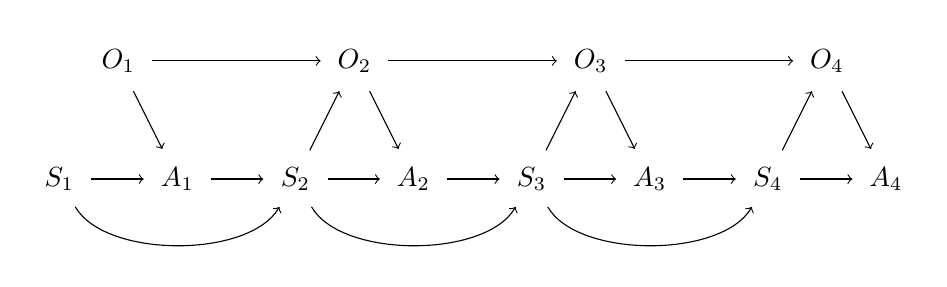
\begin{tikzpicture}
        \foreach \i in {1,2,3,4}{
            \node[circle,
                minimum size=5mm] (o-\i) at (3*\i-0.75,1.5) {$O_\i$};}
        \foreach \i in {1,2,3,4}{
            \node[circle, 
                minimum size=5mm] (a-\i) at (3*\i,0) {$A_\i$};}
        \foreach \i in {1,2,3,4}{
            \node[circle, 
                minimum size=5mm] (s-\i) at (3*\i-1.5,0) {$S_\i$};}
        \foreach \i in {1,2,3,4}{
            \draw[->] (s-\i) -- (a-\i);
            \draw[->] (o-\i) -- (a-\i);}
        \foreach \i in {2,3,4}{
            \draw[->] (s-\i) -- (o-\i);}
        \foreach \i [evaluate=\i as \j using {int(\i+1)}] in {1,2,3}{
            \draw[->] (o-\i) -- (o-\j);}
        \foreach \i [evaluate=\i as \j using {int(\i+1)}] in {1,2,3}{
            \draw[->] (a-\i) -- (s-\j);
            \path (s-\i) edge[out=-60,in=-120,looseness=0.75,->] (s-\j);}
    \end{tikzpicture}}
    \caption{Bayesian network of the HRL option framework.}
    \label{fig:Bayes_net}
\end{figure}

\subsection{The HIL Problem}

Suppose that an expert uses the HRL with options framework to generate a sequence of states and actions $\{(s_t,a_t)\}_{t = 1}^T$.
In the HIL problem, we seek to use this sequence to learn the expert's underlying low and high-level policies $\pi_{lo}$ and $\pi_{hi}$.
The associated options $\{o_t\}_{t = 1}^T$ are not observed and constitute hidden (or latent) variables.
The HIL problem is thus an instance of learning in the presence of latent variables which has motivated its solution via EM approaches in \citep{Daniel2016,zhiyu20,Giammarino_2021}.
Due to local convergence issues inherent in EM approaches, we shall take a different approach and develop a method of moments for HIL inspired by the method of moments for HMMs developed in \citep{hsu08}.

To develop our method, we define the following matrices.
\begin{definition}
    For $s \in \mathcal{S}$, define $\bm{\Pi}^{lo}_s\in\mathbb{R}^{\omega\times\alpha}$ with $$\bm{\Pi}^{lo}_s[o,a] = \pi_{lo}(A_t=a\vert O_t=o,S_t=s)$$ as the matrix representation of $\pi_{lo}$ under the state $s$.
\end{definition}

\begin{definition}
    For $s \in \mathcal{S}$, define $\bm{\Pi}^{hi}_s\in\mathbb{R}^{\omega\times\omega}$ with $$\bm{\Pi}^{hi}_s[o,o'] = \pi_{hi}(O_{t+1} = o'\vert O_t = o,S_{t+1}=s)$$
    as the matrix representation of $\pi_{hi}$ under the state $s$.
\end{definition}

\begin{definition}
    For $a \in \mathcal{A}$, define $\bm{\Phi}^A_a\in\mathbb{R}^{\zeta\times\zeta}$ with
    \[
        \bm{\Phi}^A_a[s,s']=\Phi(S_{t+1} = s'\vert S_t = s, A_t=a)
    \]
    as matrix representations of the transition dynamics.
\end{definition}

\begin{definition}
    For $s'\in\mathcal{S}$, define $\bm{\Xi}_{s'}\in\mathbb{R}^{\zeta\times\omega}$ with $$\bm{\Xi}_{s'}[s,o] = P(S_t=s,O_t=o,S_{t+1}=s').$$
\end{definition}

We also require the following mild regulatory assumptions.
\begin{assumption}[Option-Action Identifiability]\label{asu:pilo}
Under the same state, no two options contain the same policy for choosing an action, i.e., $\bm{\Pi}^{lo}_s$ has full row rank $\forall s\in\mathcal{S}$.
\end{assumption}

\begin{assumption}[Option-Option Identifiability]\label{asu:pihi}
Under the same state, no two options give the same policy for choosing the next option, i.e., $\bm{\Pi}^{hi}_s$ has full rank $\forall s\in\mathcal{S}$. 
\end{assumption}

\begin{assumption}\label{asu:invertibility}
$\bm{\Xi}_s$ has full column rank $\forall s\in\mathcal{S}$.
\end{assumption}

\begin{assumption}\label{asu:noisy_transition}
All actions have a non-zero chance of transitioning a state to all of its neighboring states and one state is another state's neighbor if there exists an action under which the probability of transitioning from the latter to the former is non-zero, i.e., for any $s,s'\in\mathcal{S}$, if there exists $a\in\mathcal{A}$ such that $\bm{\Phi}^A_a[s,s']>0$, then $\bm{\Phi}^A_{a'}[s,s']>0,\forall a'\in\mathcal{A}.$
\end{assumption}

\begin{assumption}[Stationary]\label{asu:stationary}
The process $(O_t,S_t)$ starts with the stationary distribution, that is $\bm{\pi}^1_s[o]=\bm{\pi}^\infty_s[o]$ where $\bm{\pi}^t_s\in\mathbb{R}^\omega$ with $\bm{\pi}^t_s[o]=P(O_t=o,s_t=s)$ for $s \in \mathcal{S}$.
\end{assumption}
\begin{remark}
Assumptions \ref{asu:pilo}, \ref{asu:pihi}, and \ref{asu:invertibility} follow the same line of reasoning as Condition 1 of \cite{hsu08}; they remove malicious instances that can cause learning to confuse options that have the same transition/action probability. Assumption \ref{asu:noisy_transition} is needed as the method of moments relies on the cancellation of certain terms across all actions, it can be interpreted as an action emission noise in the expert or a transition noise in the environment.
\end{remark}
% \npnguyen{Assumption \ref{asu:invertibility} can be dropped at the cost of increasing the size of the matrix $M$ from $\zeta\zeta\times\zeta\alpha$ to $\zeta\zeta\alpha\times\zeta\alpha$. What is your opinion?}

\section{Spectral method of moments}

In this section, we develop our method of moments for HIL.
We specifically identify observable moments of the states and actions, and show that they enable recovery of the low-policy $\pi_{lo}$ via matrix diagonalization and the high-level policy $\pi_{hi}$ via simple matrix algebra.

\subsection{Moments in HIL}
We note that under Assumption \ref{asu:stationary}, the moments of the states, options, and actions are time-invariant.
Thus, without loss of generality, we consider the moments $\bm{M}_a\in \mathbb{R}^{\zeta\zeta\times\zeta\alpha}$ for $a\in\mathcal{A}$ with
\[
    &\bm{M}_a\lrb{s_2\zeta+s_1,s_3\alpha+a_3}\\
        &\quad=\ P(S_2=s_2,S_1=s_1,A_2=a,S_3=s_3,A_3=a_3),
      %  \numberthis
\]
and $\bm{K}_{s}\in\mathbb{R}^{\zeta\times\alpha}$ for $s\in\mathcal{S}$ with
\[
    \bm{K}_s[s_1,a_2]
    = P(S_1=s_1,S_2=s,A_2=a_2). %\numberthis
\]
Our goal now is to construct an expression of these observable moments that allows the recovery of the low-level policy via matrix diagonalization.

\subsection{Diagonalizable Forms}

We first examine the properties of $\bm{K}_s$ for $s \in \mathcal{S}$.
Specifically, let $\bm{V}_s\in\mathbb{R}^{\alpha\times\omega}$ for $s \in \mathcal{S}$ be a matrix of right singular vectors corresponding to the $\omega$ largest singular values of $\bm{K}_s$.
We then have the following lemma.
%Finally, the proof of the core theorem makes use of the following lemma:
\begin{lemma}%[Action Projection invertibility]
\label{lem:actionProjection}
Define the block-diagonal matrices
\[\label{eq:Vmat}
    \bm{V} = \bmat{\bm{V}_1&&\\&\ddots&\\&&\bm{V}_\zeta} \text{ and } \bm{\Pi}^{lo}=\bmat{\bm{\Pi}^{lo}_1&&\\&\ddots&\\&&\bm{\Pi}^{lo}_\zeta}.
\]
Then the product matrix
\[
    \bm{\Pi}^{lo}\bm{V} = \bmat{\bm{\Pi}^{lo}_1\bm{V}_1&&\\&\ddots&\\&&\bm{\Pi}^{lo}_\zeta\bm{V}_\zeta}
\]
is invertible.
\end{lemma}
\begin{proof}
We have
\[
    \bm{K}_s[s_1,a_2]
    %=&P(S_1=s_1,S_2=s,A_2=a_2)\\
    &=\sum_{o_1}\sum_{o_2} P(O_1=o_1,S_1=s_1,S_2=s)\\
    &\qquad\times \pi_{hi}(O_2=o_2\vert O_1=o_1,S_2=s)\\
    &\qquad\times \pi_{lo}(A_2=a_2\vert O_2=o_2,S_2=s)\\
    &=\lrc{\bm{\Xi}_s\bm{\Pi}^{hi}_s\bm{\Pi}^{lo}_s}[s_1,a_2].\label{eq:overline_K_derive}
\]

This implies $\mathrm{rowspan}(\bm{K}_s)\subseteq\mathrm{rowspan}(\bm{\Pi}^{lo}_s)$. In addition, because $\bm{\Xi}_s$ is full column rank and $\bm{\Pi}^{hi}_s$ is full rank (Assumptions \ref{asu:pihi} and \ref{asu:invertibility}),
\[
    \bm{\Pi}^{lo}_s=(\bm{\Xi}_s\bm{\Pi}^{hi}_s)^+\bm{K}_s,
\]
which implies $\mathrm{rowspan}(\bm{\Pi}^{lo}_s)\subseteq\mathrm{rowspan}(\bm{K}_s)$. Thus,
\[
    \mathrm{rowspan}(\bm{V}_s\transpose)
        =\mathrm{rowspan}(\bm{K}_s)
        =\mathrm{rowspan}(\bm{\Pi}^{lo}_s).
\]
Therefore, $\bm{\Pi}^{lo}_s\bm{V}_s$ is invertible. Since $s$ is chosen arbitrarily, this applies for all $s$.
% Now consider
% \[
%     \bm{\Pi}^{lo}\bm{V} = \bmat{\bm{\Pi}^{lo}_1\bm{V}_1&&\\&\ddots&\\&&\bm{\Pi}^{lo}_\zeta\bm{V}_\zeta}.
% \]
Because $\bm{\Pi}^{lo}_s\bm{V}_s$ is invertible for all $s$, it follows that $\bm{\Pi}^{lo}\bm{V}$ is also invertible.
\hspace*{\fill} \qed
\end{proof}

We next examine the properties of the moments $\bm{M}_a$.
Before doing so, note that the moments $\bm{M}_a$ involve the transition dynamics $\bm{\Phi}^A_a$ as well as the underlying low- and high-level policies we are interested in. 
To remove the influence of the transition dynamics on $\bm{M}_a$, let us define the kernel matrix $\bm{\Psi} \in \mathbb{R}^{\zeta \times \zeta}$ with
\[
    \bm{\Psi}[s_2,s_3]&=\left\{\begin{aligned}\label{eq:psi}
        &\psi_{s_2s_3},\quad&\text{if}\ \bm{\Phi}^A_a[s_2,s_3]>0\ \forall a\in\mathcal{A},\\
        &0,\quad&\text{otherwise},
    \end{aligned}\right.
\]
and normalizer matrices $\bm{N}_a \in \mathbb{R}^{\zeta \times \zeta}$ for $a \in \mathcal{A}$ with
\[
    \bm{N}_a[s_2,s_3]&=\left\{\begin{aligned}\label{eq:normmat}
        &\frac{1}{\bm{\Phi}^A_a[s_2,s_3]},\quad&\text{if}\ \bm{\Phi}^A_a[s_2,s_3]>0,\\
        &0,\quad&\text{otherwise,}
    \end{aligned}\right.
\]
where $\psi_{s_2s_3}$ are constants of choice such that $\bm{\Psi}$ is full rank (such constants will always exist under Assumption \ref{asu:noisy_transition}). %Choosing these constants so as to minimize the sample complexity will be reserved for future works.
We then may define the surrogate moments
\[\label{eq:mathcalM}
    \bm{\hat{M}}_a = (\bm{\Psi}\otimes\one_{\zeta\times\alpha})\circ (\bm{N}_a\otimes\one_{\zeta\times\alpha})\circ \bm{M}_a,
\]
for $a \in \mathcal{A}$ and 
\[\label{eq:mathcalM_sum}
    \bm{\hat{M}} = \sum_{a\in\mathcal{A}}\bm{\hat{M}}_a
\]
that do not depend on the transition dynamics where $\bm{\hat{M}}_a$ and $\bm{\hat{M}}$ have the same dimensions as $\bm{M}_a$.

These surrogate moments combined with Lemma \ref{lem:actionProjection} lead to the following theorem that establishes that the observable moments allow the recovery of the low-level policy via matrix diagonalization.
\begin{theorem}\label{theo:central}
The product $\bm{V}\transpose\bm{\hat{M}}^+\bm{\hat{M}}_a\bm{V}$ admits the factorization:
\[\label{eq:diagonalize}
    \bm{V}\transpose\bm{\hat{M}}^+\bm{\hat{M}}_a\bm{V} = \bm{B}\inv\bm{\Lambda}_a\bm{B},
\]
where
\[\label{eq:Lambda_definition}
    \bm{\Lambda}_a = \bmat{\mathrm{diag}(\bm{\Pi}^{lo}_1\unit_a)&&\\
              &\ddots&\\
              &&\mathrm{diag}(\bm{\Pi}^{lo}_{\zeta}\unit_a)}.
\]
\end{theorem}
\begin{proof}
% Let us define
% \[
%     \bm{\Xi}\lrb{s_2\zeta+s_1, s_2'\omega+o_1}
%     &=\ P(O_1=o_1,S_1=s_1,S_2=s_2=s_2')\notag\\
%     &=\ \begin{cases}
%             \bm{\Xi}_{s_2}[s_1,o_1]\ &\text{if}\ s_2=s_2'\\
%             0\ &\text{otherwise}.
%         \end{cases}
% \]
Let 
\[
    \bm{\Xi}=\bmat{\bm{\Xi}_1&&\\&\ddots&\\&&\bm{\Xi}_\zeta}
    \text{ and } \bm{\Pi}^{hi}=\bmat{\bm{\Pi}^{hi}_1&&\\&\ddots&\\&&\bm{\Pi}^{hi}_\zeta}.
\]
% Next, we define
% \[
%     &\bm{\Pi}^{lo}[s_1\omega+o_1,s_1'\alpha+a_1]\\
%     =\ &\pi_{lo}(A_1=a_1,S_1=s_1'\vert O_1=o_1,S_1=s_1)\\
%     =\ &\left\{\begin{aligned}
%         &\bm{\Pi}^{lo}_{s_1}[o_1,a_1]\ &\text{if}\ s_1=s_1'\\
%         &0\ &\text{otherwise}
%     \end{aligned}\right. ,\numberthis
% \]
% \[
%     &\bm{\Pi}^{hi}[s_2\omega+o_1,s_2'\omega+o_2]\\
%     =\ &\pi_{hi}(O_2=o_2,S_2=s_2'\vert O_1=o_1,S_2=s_2)\\
%     =\ &\left\{\begin{aligned}
%         &\bm{\Pi}^{hi}_{s_2}[o_1,o2]\ &\text{if}\ s_2=s_2'\\
%         &0\ &\text{otherwise}
%     \end{aligned}\right. .\numberthis
% \]

% As defined in \eqref{eq:Lambda_definition},
% \[
%     \bm{\Lambda}_a = \bmat{\mathrm{diag}(\bm{\Pi}^{lo}_1\unit_a)&&\\
%               &\ddots&\\
%               &&\mathrm{diag}(\bm{\Pi}^{lo}_{\zeta}\unit_a)}.
% \]

% The entries of $\bm{\Lambda}_a$ can be interpreted as
% \begin{multline}
%     \bm{\Lambda}_a[s_t\omega+o_t,s_t'\omega+o_t']\\
%     =\pi_{lo}(A_1=a_1,S_t=s_1',O_1=o_1'\vert O_1=o_1,S_t=s_1)
% \end{multline}
Then,
\[
  &\bm{M}_a\lrb{s_2\zeta+s_1,s_3\alpha+a_3}\\
  %=\ &P(S_2=s_2,S_1=s_1,A_2=a,S_3=s_3,A_3=a_3)\\
  =\ &\sum_{s_2',o_1}
      \sum_{s_2'',o_2}
      \sum_{s_2''', o_2'}
      \sum_{s_3, o_2'}
      \sum_{s_3', o_2''}\\
  &\qquad \phantom{\times}\ P(O_1=o_1,S_1=s_1,S_2=s_2=s_2')\\
  &\qquad \times\pi_{hi}(O_2=o_2,S_2=s_2''\vert O_1=o_1,S_2=s_2')\\
  &\qquad \times\pi_{lo}(A_2=a,S_2=s_2''',O_2=o_2'\vert O_2=o_2, S_2=s_2'')\\
  &\qquad \times P(S_3=s_3,O_2=o_2''\vert A_2=a,S_2=s_2''', O_2=o_2')\\
  &\qquad \times\pi_{hi}(O_3=o_3,S_3=s_3'\vert O_2=o_2'',S_3=s_3)\\
  &\qquad \times\pi_{lo}(A_3=a_3,S_3=s_3''\vert O_3=o_3,S_3=s_3')\\
  =\ &\lrc{\bm{\Xi}\bm{\Pi}^{hi}\bm{\Lambda}_a(\bm{\Phi}^A_a\otimes
      \identity_\omega)\bm{\Pi}^{hi}\bm{\Pi}^{lo}}
  \lrb{s_2\zeta+s_1,s_3\alpha+a_3}.%\numberthis
\]
Consider the $\zeta\times\alpha$ submatrix
\[
    \bm{U}^a_{s_2s_3}[s_1, a_3] &= 
        \bm{M}_a[s_2\zeta+s_1,s_3\alpha+a_3]\\
    \Leftrightarrow \bm{U}^a_{s_2s_3} &=
        \bm{\Xi}_{s_2}\bm{\Pi}^{hi}_{s_2}\mathrm{diag}(\bm{\Pi}^{lo}_{s_2}\unit_a)
        \bm{\Phi}^A_a[s_2,s_3]\bm{\Pi}^{hi}_{s_3}\bm{\Pi}^{lo}_{s_3}. %\numberthis
\]
Notice that $\bm{\Phi}^A_a[s_2,s_3]$ is a real number that can be estimated using observable data. We define
\[
    \bm{\hat{U}}^a_{s_2s_3} &= \frac{1}{\bm{\Phi}^A_a[s_2,s_3]}\bm{U}^a_{s_2s_3} \\
    &=\bm{\Xi}_{s_2}\bm{\Pi}^{hi}_{s_2}\mathrm{diag}(\bm{\Pi}^{lo}_{s_2}\unit_a)
        \bm{\Pi}^{hi}_{s_3}\bm{\Pi}^{lo}_{s_3} \label{eq:sub_mathcalM}
\]
 for all $s_2, s_3\in\mathcal{S}$ such that $\bm{\Phi}^A_a[s_2,s_3]>0, \forall a\in\mathcal{A}$, and $\bm{\hat{U}}^a_{s_2s_3} = \zero_{\zeta\times\alpha}$ otherwise.


By the Definitions (\ref{eq:mathcalM},~\ref{eq:sub_mathcalM})
\[
    \bm{\hat{M}}_a &=(\bm{\Psi}\otimes\one_{\zeta\times\alpha})\circ\bmat{\bm{\hat{U}}^a_{11}
        &\dots&\bm{\hat{U}}^a_{1\zeta}\\
    \vdots&\ddots&\vdots\\ \bm{\hat{U}}^a_{\zeta 1}&\dots&\bm{\hat{U}}^a_{\zeta\zeta}}\\
    &=\bm{\Xi}\bm{\Pi}^{hi}\bm{\Lambda}_a
        (\bm{\Psi}\otimes \identity_\omega)\bm{\Pi}^{hi}\bm{\Pi}^{lo}.%\numberthis
\]

By the Definition \eqref{eq:mathcalM_sum}
\[
    \bm{\hat{M}} &= \sum_{a\in\mathcal{A}}\bm{\hat{M}}_a\\
    &=\bm{\Xi}\bm{\Pi}^{hi}\lrp{\sum_{a\in\mathcal{A}}\bm{\Lambda}_a}
        (\bm{\Psi}\otimes \identity_\omega)\bm{\Pi}^{hi}\bm{\Pi}^{lo}\\
    &=\bm{\Xi}\bm{\Pi}^{hi}(\bm{\Psi}\otimes \identity_\omega)\bm{\Pi}^{hi}\bm{\Pi}^{lo}.%\numberthis
\]
Finally, we can write Equation \eqref{eq:diagonalize} as
\[
    &\bm{V}\transpose\bm{\hat{M}}^+\bm{\hat{M}}_a\bm{V}\\
    =&\lrp{\bm{\Pi}^{hi}\bm{\Pi}^{lo}\bm{V}}\inv
        \lrp{\bm{\Psi}\inv\otimes\identity_\omega}
        \bm{\Lambda}_a(\bm{\Psi}\otimes \identity_\omega)
        \bm{\Pi}^{hi}\bm{\Pi}^{lo}\bm{V},\label{eq:diagonalize_detailed}
\]
and the proof is complete.
\hspace*{\fill} \qed
\end{proof}

In order to compute the eigenbasis that jointly diagonalize \eqref{eq:diagonalize} for all $a\in\mathcal{A}$, we find a vector $\bm{\eta}\in\mathbb{R}^{\alpha}$ such that the eigenvalues of
\[\label{eq:jointDiag}
    \sum_{a\in\mathcal{A}}\bm{\eta}_a\bm{V}\transpose\bm{\hat{M}}^+\bm{\hat{M}}_a\bm{V}=
    \bm{B}\lrp{\sum_{a\in\mathcal{A}}\bm{\eta}_a\bm{\Lambda}_a}\bm{B}\inv
\]
are well spread. In other words, we find $\bm{\eta}$ such that the values $\unit_o\transpose\bm{\Pi}^{lo}_s\bm{\eta}$ are distinct and non-zero for all $(o,s)\in\mathcal{O}\times\mathcal{S}$. As suggested in \cite{HsuKakade13}, this can be satisfied in most cases if $\bm{\eta}$ is sampled uniformly from the surface of a unit sphere in $\mathbb{R}^\alpha$.

The eigen-decomposition will yield an eigenbasis up to a permutation $\bm{\mathcal{P}}\in\mathbb{R}^{\omega\times\zeta}$ of the pair $(o,s)\in\mathcal{O}\times\mathcal{S}$. To put it differently, the diagonal matrix obtained from diagonalizing $\bm{V}\transpose\bm{\hat{M}}^+\bm{\hat{M}}_a\bm{V}$ using this basis will be of the form
$\bm{\mathcal{P}}\bm{\Lambda}_a\bm{\mathcal{P}}\transpose$.
With some further processing, an order up to a permutation $\bm{\hat{\mathcal{P}}}\in\mathbb{R}^\omega$ of $o\in\mathcal{O}$ can be recovered, meaning the diagonal matrix obtained will be of the form $(\identity_\zeta\otimes\bm{\hat{\mathcal{P}}})\bm{\Lambda}_a(\identity_\zeta\otimes\bm{\hat{\mathcal{P}}}\transpose)$. This ordering corresponds to the relabeling of the options. Because this recovery process, while necessary, does not represent the main contribution of this work, it will be elaborated in the Appendix.

After obtaining the low-level policy matrices $\bm{\hat{\mathcal{P}}}\bm{\Pi}^{lo}_s$, the high-level policy matrices can be computed by the following theorem, up to the permutation $\bm{\hat{\mathcal{P}}}$ of the options.
\begin{theorem}
\[\label{eq:pihi_recovery}
    \bm{\hat{\mathcal{P}}}\bm{\Pi}^{hi}_{s'}\bm{\hat{\mathcal{P}}}\transpose=
        \sum_s \bm{w}_{s'}[s]\lrp{\bm{\hat{\mathcal{P}}}\bm{\Pi}^{lo}_s
        \bm{K}_s^+\bm{\hat{K}}_{ss'}
        {\bm{\Pi}^{lo}_{s'}}^+\bm{\hat{\mathcal{P}}}\transpose},
\]
where:
\begin{itemize}
    \item $\bm{\hat{K}}_{ss'}$ is a $\zeta\times\alpha$ submatrix of $\bm{\hat{M}}$ defined by
    \[\label{eq:hat_K_definition}\citep{Bauer:2007}
        \bm{\hat{K}}_{ss'}[s'',a]=\bm{\hat{M}}[s\zeta+s'',s'\alpha+a].
    \]
    \item $\bm{w}_{s'}$ are length $\zeta$ weight vectors of choice subject to
    \[\label{eq:pihi_weight_constraint}
        \bm{w}_i\transpose\bm{\Psi} \unit_i\transpose=1,\ \forall i\in\mathcal{S}.
    \]
\end{itemize}
\end{theorem}
\begin{proof}
According to Definition \eqref{eq:hat_K_definition} and Equation \eqref{eq:overline_K_derive}, $\bm{K}_s$ and $\bm{\hat{K}}_{ss'}$ can be written as following:
\[
    \bm{K}_s = \bm{\Xi}_s\bm{\Pi}^{hi}_s\bm{\Pi}^{lo}_s,
\]
\[
    \bm{\hat{K}}_{ss'} = \bm{\Psi}[s,s']\lrp{\bm{\Xi}_s\bm{\Pi}^{hi}_s\bm{\Pi}^{hi}_{s'}\bm{\Pi}^{lo}_{s'}}.
\]
Therefore,
\[
    &\bm{\Pi}^{lo}_s{\bm{K}_s}^+\bm{\hat{K}}_{ss'}{\bm{\Pi}^{lo}_{s'}}^+\\
    =\ &\bm{\Psi}[s,s']\lrp{\bm{\Pi}^{lo}_s{\bm{\Pi}^{lo}_s}^+{\bm{\Pi}^{hi}_s}\inv
        {\bm{\Xi}_s}^+\bm{\Xi}_s\bm{\Pi}^{hi}_s\bm{\Pi}^{hi}_{s'}\bm{\Pi}^{lo}_{s'}{\bm{\Pi}^{lo}_{s'}}^+}\\
    =\ &\bm{\Psi}[s,s']\bm{\Pi}^{hi}_{s'}.%\numberthis
\]
With that, we contract the left hand side of Equation \eqref{eq:pihi_recovery}
\[
    &\sum_s \bm{w}_{s'}[s]\lrp{\bm{\hat{\mathcal{P}}}\bm{\Pi}^{lo}_s\bm{K}_s^+\bm{\hat{K}}_{ss'}
        {\bm{\Pi}^{lo}_{s'}}^+\bm{\hat{\mathcal{P}}}\transpose}\\
    =&\sum_s \bm{w}_{s'}[s]\bm{\Psi}[s,s']\lrp{\bm{\hat{\mathcal{P}}}\bm{\Pi}^{hi}_{s'}
        \bm{\hat{\mathcal{P}}}\transpose}\\
    =&\bm{\hat{\mathcal{P}}}\bm{\Pi}^{hi}_{s'}{\bm{\hat{\mathcal{P}}}}\transpose.
    %\numberthis
\]
The last equality holds because we chose $\bm{w}_{s'}$ such that $\sum_s \bm{w}_{s'}[s]\bm{\Psi}[s,s']=1$. Analysis of the choice of $\bm{w}_{s'}$ will be reserved for future work.
\hspace*{\fill} \qed
\end{proof}

\subsection{Proposed Method of Moments for HIL}
Given the observed sequence $\{(s_t,a_t)\}_{t = 1}^T$, our method of moments to learn the policies $\pi_{lo}$ and $\pi_{hi}$ is:
\begin{enumerate}[leftmargin=2cm, label=Step \arabic*:]
    \item Estimate $\bm{M}_a$, $\bm{K}_s$, and $\bm{\Phi}^A_a$ from data via:
    \[
        &\bm{M}_a\lrb{s_2\zeta+s_1,s_3\alpha+a_3}\\
        =\ &\frac{\sum_{t=1}^{T-2}\indicator{s_t=s_1,s_{t+1}=s_2,a_{t+1}=a,s_{t+2}=s_3,a_{t+2}=a_3}}{T-2},
            %\numberthis 
            \\
        &\bm{K}_s\lrb{s_1,a_2}
        =\ \frac{\sum_{t=1}^{T-1}\indicator{s_t=s_1,s_{t+1}=s,a_{t+1}=a_2}}{T-1},
            %\numberthis
    \]
    \[
        \bm{\Phi}^A_a[s,s'] &= \frac{\sum_{t=1}^{T-1}\indicator{s_t=s, a_t=a, s_{t+1}=s'}}{\sum_{t=1}^{T-1}\indicator{s_t=s, a_t=a}}.
    \]
    \item Compute the surrogate moments $\bm{\hat{M}}_a$ and $\bm{\hat{M}}$ according to Equations \eqref{eq:mathcalM} and \eqref{eq:mathcalM_sum}.

    \item Perform SVD on $\bm{K}_s$, and construct the matrix $\bm{V}$ according to Equation \eqref{eq:Vmat}.
    \item Compute the joint eigenbasis $\bm{B}$ using Equation \eqref{eq:jointDiag}. Then, recover the order of its column using the algorithm discussed in the Appendix.
    \item Recover $\bm{\Pi}^{lo}$ using the diagonals that result from diagonalizations according to Equation \eqref{eq:diagonalize}.
    \item Compute $\bm{\Pi}^{hi}$ with Equation \eqref{eq:pihi_recovery}.
\end{enumerate}

\subsection{Performance discussion}
The algorithm consists of two parts, data collection with complexity $\mathcal{O}(T)$, and data processing with complexity $\mathcal{O}(\zeta^4\alpha\omega)$, dominated by the cost of computing $\bm{V}\transpose\bm{\hat{M}}^+\bm{\hat{M}}_a\bm{V}$ and its eigenbasis. This gives us the total time complexity of $\mathcal{O}(T+\zeta^4\alpha\omega)$.

Comparison to the EM methods presented in \cite{zhiyu20} and \cite{Giammarino_2021}, which has time complexity of $\mathcal{O}(T\omega^2)$ and $\mathcal{O}(\zeta\alpha\omega^3)$ per iteration respectively, can be difficult. This is due to the fact that they have different bottlenecks, along with the fact that the method of moments is parameter-less while EM methods need initialization. However, a general rule is that the larger the number of samples is relative to the number of states and actions, the better the method of moments performs compared to EM.

Another thing to note is that the techniques mentioned can be synergistic, with the output of the method of moments being good initialization for EM methods to refine.
\section{Experiment}
In this section, we examine the proposed algorithm in numerical experiments.
We will use a similar setup to \cite{zhiyu20} to test our model. Let there be a finite state machine with four states and the following parameters:
\[
    \bm{\Pi}^{hi}_1=\bmat{0.67&0.33\\0.16&0.84},\quad
    \bm{\Pi}^{hi}_2=\bmat{0.88&0.12\\0.16&0.84},\\
    \bm{\Pi}^{hi}_3=\bmat{0.84&0.16\\0.12&0.88},\quad
    \bm{\Pi}^{hi}_4=\bmat{0.84&0.16\\0.33&0.67}.%\numberthis
\]
\[
    \bm{\Pi}^{lo}_1=\bmat{0.6&0.4\\0.1&0.9},\quad
    \bm{\Pi}^{lo}_2=\bmat{0.7&0.3\\0.15&0.85},\\
    \bm{\Pi}^{lo}_3=\bmat{0.8&0.2\\0.3&0.7},\quad
    \bm{\Pi}^{lo}_4=\bmat{0.9&0.1\\0.35&0.65}.%\numberthis
\]
\[
    \bm{\Phi}^A_1=\bmat{0.7&0.1&0.1&0.1\\
        0.4&0.4&0.1&0.1\\0.3&0.3&0.3&0.1\\
        0.25&0.25&0.25&0.25},\\
    \bm{\Phi}^A_2=\bmat{0.25&0.25&0.25&0.25\\
        0.1&0.3&0.3&0.3\\0.1&0.1&0.4&0.4\\
        0.1&0.1&0.1&0.7}.%\numberthis
\]

The error will be measured by:
\[
    \mathrm{ERROR}=\sqrt{\norm{\bm{\Pi}^{lo}-\overline{\bm{\Pi}}^{lo}}^2_2
        +\norm{\bm{\Pi}^{hi}-\overline{\bm{\Pi}}^{hi}}^2_2},
\]
where $\overline{\bm{\Pi}}^{lo},\overline{\bm{\Pi}}^{hi}$ are the predicted values of $\bm{\Pi}^{lo},\bm{\Pi}^{hi}$.

For intuition, we can think of the states as locations on a number line (i.e., states with larger index are further right), the actions are $\mathcal{A}=\{\textrm{move-left},\textrm{move-right}\}$, and the options are $$\mathcal{O}=\{\textrm{tend-to-move-left},\textrm{tend-to-move-right}\}.$$ Looking at the numbers, we can see that the agent wants to alternately move from left to right and right to left.

\begin{figure}
    \centering
    \resizebox{0.4\textwidth}{!}{\begin{tikzpicture}
    \begin{loglogaxis}[
        width = 0.5\textwidth,
        height = 0.25\textwidth,
        xlabel = {$T$},
        ylabel = {$\mathrm{ERROR}$},]
     
    % Plot data from a file
    \addplot[
        thin,
        red,
    ] file[] {figures/sample_error.txt};
    \addplot[
        thin,
        blue,
    ] file[] {figures/sample_error_2.txt};
    \addplot[
        thin,
        green,
    ] file[] {figures/sample_error_3.txt};
     
    \end{loglogaxis}
 
    \end{tikzpicture}}
    \caption{Log-log plot of the error versus the number of sample points for several realizations of the problem.}
    \label{fig:error}
\end{figure}


In Fig.\ \ref{fig:error} we plot the error versus the number of samples for a few runs of our method in log scale. It can be seen that the error is polynomial relative to the number of samples.

For comparison purposes, Fig.\ \ref{fig:EM_error} depicts a few EM runs with randomized initialization and a sample size of $3 \times 10^5$. It can be seen that initialization have a significant effect on EM's rate of convergence and whether or not it arrives at the correct optima. In contrast, the proposed method of moments does not require initialization.
\begin{figure}
    \centering
    \resizebox{0.4\textwidth}{!}{\begin{tikzpicture}
    \begin{semilogyaxis}[
        width = 0.5\textwidth,
        height = 0.25\textwidth,
        xlabel = {Iterations},
        ylabel = {$\mathrm{ERROR}$},]
     
    % Plot data from a file
    \addplot[
        thin,
        red,
    ] file[] {figures/plot_2_0_300000.txt};
    \addplot[
        thin,
        green,
    ] file[] {figures/plot_2_1_300000.txt};
    \addplot[
        thin,
        blue,
    ] file[] {figures/plot_2_2_300000.txt};
    \addplot[
        thin,
        black,
    ] file[] {figures/plot_2_3_300000.txt};
    \addplot[
        thin,
        orange,
    ] file[] {figures/plot_2_4_300000.txt};
    \addplot[
        thin,
        cyan,
    ] file[] {figures/plot_2_5_300000.txt};
     
    \end{semilogyaxis}
 
    \end{tikzpicture}}
    \caption{Iterations versus error of EM runs with various initializations, some of which do not converge.}
    \label{fig:EM_error}
\end{figure}

\section{Conclusions and Future Work}
\label{sec:conclusions}
We developed a novel method of moments for Hierarchical Imitation Learning (HIL) that offers global convergence under mild regulatory conditions.
Our method of moments for HIL is based on similar methods for HMMs and other latent variable models, and avoids the local convergence issues inherent in previous Expectation-Maximization (EM) approaches to HIL.
Future work could include further relaxation of the conditions under which the method holds and examining its extension to situations in which the options form a semi-Markov (rather than a Markov) process.

\section{Introduction}
\label{sec:intro}

Characterizing latent structures with meaningful real-world interpretations is a central task in statistics.
In scientific applications, this task often amounts to discovering unobserved physical ``processes'' that generate observable quantities.
%To be concrete, consider two common classes of models aimed at the discovery of latent processes (although our setting and methods will be more general. 
For example, processes might correspond to subpopulations that cannot be directly observed such as
types of cells \citep{Gorsky:2020,Prabhakaran:2016}, behavioral genotypes \citep{Stevens:2019}, or
groups with canonical patterns of IQ development \citep{Bauer:2007}.
Also, processes could correspond to a variety of scientifically important objects such cell programs \citep{Kotliar_Identify_Cell_Idendity_Activity_NMF_2019,Buettner_FscLVM_ScalableVersatile_FA_2017,Risso_General_Flexible_Signal_Extract_2018},
mutational processes in tumors %(e.g., using whole genome sequencing data) 
\citep{Levitin_DeNovo_Gene_Signature_Identification_2019,Kinker_Pan_Cancer_2020,Seplyarskiy_PopulationSequencingData_2021},
or material types
\citep{Fevotte_NonlinearHyperspectralUnmixing_2015,Rajabi_SpectralUnmixingHyperspectral_2015}.

In practice, it is necessary to not only characterize each latent process but also determine \emph{how many} such processes there are.
This requires solving a model selection problem for a sequence of model families $\model{K} = \{ P_\theta : \theta \in \Theta_K\}$, $K = 1, 2, \dots,$ where $K$ denotes the number of latent processes in the model.
For example, $K$ could be the number of components in a mixture model or the number of factors in a factor analysis model.
Given some observed data $\data{1},\dots, \data{N} \distiid P_o$ that were generated by the output of $K_{o}$ latent processes,
the goal is to recover $K_{o}$ and a model $\widetilde{P}_o \in \model{K_{o}}$ such that $\widetilde{P}_o  \approx P_{o}$.
Standard frequentist and Bayesian model selection methods provide consistent estimation of $K_o$ when $\model{K_o}$ is \emph{well-specified} (that is, $P_o \in \model{K_o}$ but $P_o \notin \model{K}$ if $K < K_o$).
However, if $\model{K_o}$ is \emph{misspecified} (that is, $P_o \notin \model{K_o}$), then standard methods do not work as intended
\citep{Cai:2021,Guha:2021,Fruhwurth:2006,Miller:2019,Xue:2024}.
The reason for this failure is that these methods optimize for some measure of \emph{predictive performance} (e.g., some form of expected log loss).
Therefore, as $N \to \infty$, these methods will select a sequence of models that converge to the distribution $P_\star
	\in \model{\infty} = \bigcup_{K=1}^\infty \model{k}$ that has minimal Kullback--Leibler divergence between $P_o$ and all $P \in \model{\infty}$.
Since typically $P_\star \notin \model{K}$ for any finite $K$, when using a predictive method for
model selection, as the number of observations $N$ increases, rather than obtaining better estimates, the opposite occurs:
the distribution $P_o$ is better estimated by adding spurious latent structures that compensate for the shortcomings of the parametric model.
This problem is known as \emph{overfitting}  \citep{Cai:2021}. %

However, when trying discover real-world processes, the statistical problem is no longer predictive in nature, but rather \emph{explanatory}  \citep{Shmueli:2010}.
The aim is to infer meaningful constructs that capture the underlying causal structure 
-- in this case the latent processes -- even if doing so results in a fitted model with reduced
predictive power.
Hence, there is a need for robust model selection procedures that can replace current defaults such as the Akaike, Bayesian, and deviance information criteria \citep{Akaike:1974,Schwarz:1978,Spiegelhalter:2002}, which remain widely used due to their simplicity and the ease with
which they can be incorporated into data analysis workflows -- for example, when a user wants to use an existing (perhaps specialized) method to estimate the parameters of each model $\model{K}$ ($K = 1, 2, \dots$).
We defer a more detailed discussion of related work until after we describe 
out methodology. 


\paragraph{Contributions.}
In this paper, we make the following contributions to the development of more reliable
and robust methods for model selection for discovering real-world latent processes:
%overcome the limitations of existing approaches:
\begin{enumerate}
	%	\item We define a broad class of generative models (\cref{sec:motivation}) .
	%	      The key modeling assumption is that each latent process generates independent latent data for each observation;
	%	      the latent data from the processes are then combined to produce the observed data.
	%	      The class includes mixture models and factor models as special cases.
    \item We define a formal notion of \textit{robust model selection consistency}
    and argue that it captures key features any robust model selection method 
    should satisfy. 
	\item We propose the \emph{accumulated cutoff discrepancy criterion} (\methodname), as a simple, flexible approach to robust model selection. 
	\item We show how to apply \methodname to a broad class of models
	in which the observations are determined by combining (unobserved) outputs from $K$ latent processes.
	% \methodname combines ideas from minimum distance estimation and coarsening, and
	% can incorporate expert and prior knowledge about the nature of the model misspecification.
	%       \methodname can be used with any parameter estimation technique, so it is easy to incorporate
	      % into existing data analysis workflows. % (see \cref{sec:case-study} for a comprehensive illustration of this).
	      %      Our minimum distance approach enables the use of any discrepancy measure between distributions,
	      %     which can be chosen in an application-specific manner.
	      %    Given fitted models each possible number of components, the computational cost required to compute our criterion is determined by the cost of estimating the discrepancy measure, which is typically quite small.
	\item We prove that \methodname provides robust model selection 
    consistency for mixture models and probabilistic matrix factorization models, including factor analysis models. 
	      %for our model class (\cref{sec:motivation}).
	      %   We show that, under intuitive assumptions, our procedure is robustly consistent (\cref{sec:theory}), 
	      % as illustrated in the third row of \cref{fig:motivate-comparison}.
	\item We demonstrate the broad utility of \methodname through four numerical experiments using mixture and matrix factorization models
	      applied to simulated and real data.\footnote{Code to reproduce all experiments is available on GitHub: \url{https://github.com/TARPS-group/robust-model-selection-for-discovery}.} % (\cref{sec:experiments}).
	      % Experiments include cell type discovery using flow cytometry data and mutational process discovery using Poisson nonnegative matrix factorization.
	      We also provide an in-depth case study that shows our criterion provides state-of-the-art clustering accuracy of single-cell RNA-seq gene expression data.
          % ~(\cref{sec:case-study})
	% \item We conclude in \cref{sec:discussion} with a discussion of some limitations of our approach and directions for future work.
\end{enumerate}



\section{Methodology}
\label{sec:methods}

We first define robust model selection consistency, which naturally 
leads to a plug-in procedure, the accumulated cutoff discrepancy criterion (\methodname). 
We then describe how to apply \methodname for a broad class of latent
variable models.
In this section, we use mixture modeling as a running example to illustrate ideas. 
Let $\mcF = \{ F_{\phi} \mid \phi \in \Phi \}$ denote the component distribution family
and let $\eta \in \Delta_{\numcomps}$ denote the component weights, 
where $\Delta_\numcomps = \{ \eta \in \reals_{+}^{\numcomps} \mid \sum_{k=1}^{\numcomps} \eta_{k} = 1 \}$ 
is the $(\numcomps-1)$-dimensional probability simplex. 
Denote the parameter set for the $\numcomps$-component mixture distributions by 
$\Theta^{(\numcomps)} = \Delta_{\numcomps} \times \Phi^{\numcomps}$, so the 
mixture model distribution family is 
\[
\model{K} = \textstyle \left\{ P_\theta = \sum_{k=1}^K \eta_k F_{\phi_k} : \theta = (\eta, \phi_1,\dots,\phi_K) \in \Theta^{(\numcomps)}\right\}. 
\]
Recall that we can also write the generative process of the mixture model in terms of
latent variables $z_{n} \in \{1,\dots,K\}$ that indicate which component observation $n$ belongs to:
\[
z_n \mid \theta &\distas \distCat(\eta) &
x_n \mid z_n = k, \theta &\distas F_{\phi_{k}}. 
\]
Since we are interested in isolating contribution of each component, it is this latent variable
representation that will be most relevant. 
We discuss applications to other models in \cref{sec:framework,sec:pmf-applications}.

\subsection{Robust Model Selection Consistency} \label{sec:robust-consistency}

Generalizing the mixture model setting, consider a sequence of models $\model{1}, \model{2}, \dots, \model{K}, \dots$, where $K$ captures how many distinct latent components are generating the observed data.
Assume that $\model{K} = \{ P_{\theta} \mid \theta \in \paramSpace{K} \}$, where $\paramSpace{K}$ is the parameter space
and $P_{\theta} \in \mcP(\mathbb{X})$, the space of probability measures on the observation space $\mathbb{X}$. 
The objective is to identify the true number of processes $K_o$.
% as well as a model $P_\star \in \model{K_o}$ that fits the data well.
Fix a \emph{distribution-level discrepancy} $\distDisc$ on probability measures that will quantify the fit between $P_{\theta}$ and the data-generating distribution $P_{o}$.
We do not assume a unique minimizing parameter since, at the very least, 
the component indices in latent variable models are non-identifiable. 
Let $\Theta_{\star}^{(K)}(P_{o}) \defas \argmin_{\theta \in\paramSpace{K}} \distDisc(P_{o} \mid P_{\theta})$ 
denote the set of minimizing parameters.
Alternatively, a practitioner might choose a parameter estimation procedure that is not model-based, in which case it might converge to a parameter value in some other set, which we also denote by $\Theta_{\star}^{(K)}(P_{o})$.
%We will formally define robust model selection consistency in terms of the set-valued function $\Theta_{\star}(P_{o}, K) \defas \Theta_{\star}^{(K)}(P_{o})$. 

The challenge in the misspecified setting is that for any $\theta_{\star}^{(K)} \in \Theta_{\star}^{(K)}(P_{o})$, typically $\distDisc(P_{o} \mid P_{\theta_{\star}^{(K)}})$ is not minimized at $K = K_{o}$.
In fact, in our settings of interest $\model{K} \subsetneq \model{K+1}$ but $P_{o} \notin \model{K}$ for any $K$, so
$\distDisc(P_{o} \mid P_{\theta_{\star}^{(K)}})$ is monotonically decreasing as $K$ increases. 
To correctly recover $K_{o}$, the user must specify how much $P_{\theta}$ can deviate from $P_{o}$ while remaining an acceptable approximation.
Therefore, we introduce a second discrepancy which measures how well the \emph{components} of $P_{o}$ and $P_{\theta}$ match.
%deviates from the assumed model and allow for some positive degree of discrepancy. 

Since the components of $P_{o}$ are unknown, the component contributions must be estimated based on model $P_{\theta}$ but 
using the distribution of data from $P_{o}$. 
Let the \emph{component-level realized discrepancy} $\compDisc^{(K)}(\theta, k, P_{o})$ quantify
how close the inferred component $k \in \{1,\dots,K\}$ from $P_{o}$ is to component $k$ of the model
$P_{\theta}^{(K)}$. 
To quantify the overall degree of component-level misspecification of $P_o$ with true number of components $K_o$,
%for a fixed choice of inference algorithm, 
define the \emph{worst-case component-wise discrepancy}
\[
 \rho(P_{o}, K_{o}) \defas  \sup_{\theta \in \Theta_{\star}^{(K_{o})}(P_{o})} \max_{k \in [K_{o}]} \compDisc^{(K_{o})}(\theta, k, P_{o}).
\]
For example, in the mixture model case we can construct a component-level realized discrepancy by inferring
the component of $P_o$ that would correspond to each mixture component.
That is, if we assign each observation from $P_o$ according to the conditional component probabilities 
$p(k \mid x, \theta) = \eta_{k} \frac{\dee F_{\phi_k}}{\dee P_{\theta}}(x)$, 
then the inferred $k$th component of $P_o$ is 
\begin{align}
	\widetilde{F}^{(\theta)}_{ok} = \frac{p(k \mid x, \theta)}{\int p(k \mid y, \theta) P_o(\dee y)} P_o. 
\end{align}
Given a choice discrepancy measure $\mcD$ (e.g., $\distDisc$), we can set 
$
\compDisc^{(K)}(\theta, k, P_{o}) = \mcD(\widetilde{F}^{(\theta)}_{ok} \mid F_{\phi_k}).
$

\begin{definition}[Robust model selection consistency] \label{def:robust-consistency}
	Fix a function $\kappa : \reals_{+} \times \nats \to \reals_{+}$. 
	A model selection procedure $\widehat K(\data{1:N}, \rho) \in \nats$ is \emph{$\kappa$-robustly consistent for $\Theta_{\star}$ and $\compDisc$} if,
	for any data-generating distribution $P_o$ and true component number $K_o$ that satisfies 
	\[ \label{eq:mismatch-condition}
		\inf_{\theta \in \Theta_{\star}^{(K)}(P_{o})} \distDisc(P_{o} \mid P_{\theta}) \ge \kappa(\rho(P_{o}, K_{o}), K)
		\quad\text{for all $K \in \{1,\dots,K_{o}-1\}$},
	\]
	it holds that, for $\data{1}, \data{2}, \dots \distiid P_{o}$, 
	\[
		\Pr\big\{\widehat K(\data{1:N}, \rho(P_{o}, K_{o})) = K_o \big\} \overset{N \to \infty}{\longrightarrow} 1.
	\]
\end{definition}
%The model selection rule can depend on $\rho =  \rho(P_{o}, K_{o})$ since $\rho$ is not inferable using samples from $P_{o}$.
To interpret \cref{def:robust-consistency} and the role of the function $\kappa$, 
it is helpful to compare robust model selection consistency to classical model selection consistency.
\Cref{fig:consistency-illustration} provides a cartoon illustration of the differences between the two types of consistency. 
Classical model consistency typically requires that  
(1) $P_o \in \model{K_o}$ and (2) $P_{o} \notin \model{K}$ for $K < K_o$ \PROBLEM{add citations}.
Robust consistency weakens the first condition by allowing for a worst-case discrepancy $\rho(P_{o}, K_{o}) \ne 0$,
whereas classical consistency would require $\rho(P_{o}, K_{o}) = 0$.
However, robust consistency strengthens the second second by requiring a gap between $P_o$ 
and all models for $K < K_o$.
The size of this gap specified in \cref{eq:mismatch-condition} in terms of $\kappa$. 
Hence, we call $\kappa$ the \emph{gap function}. 
It would be natural to ask that $\kappa(\rho, K) = \rho$, although this may not always be possible. 

\begin{figure}[tp]
	\centering
	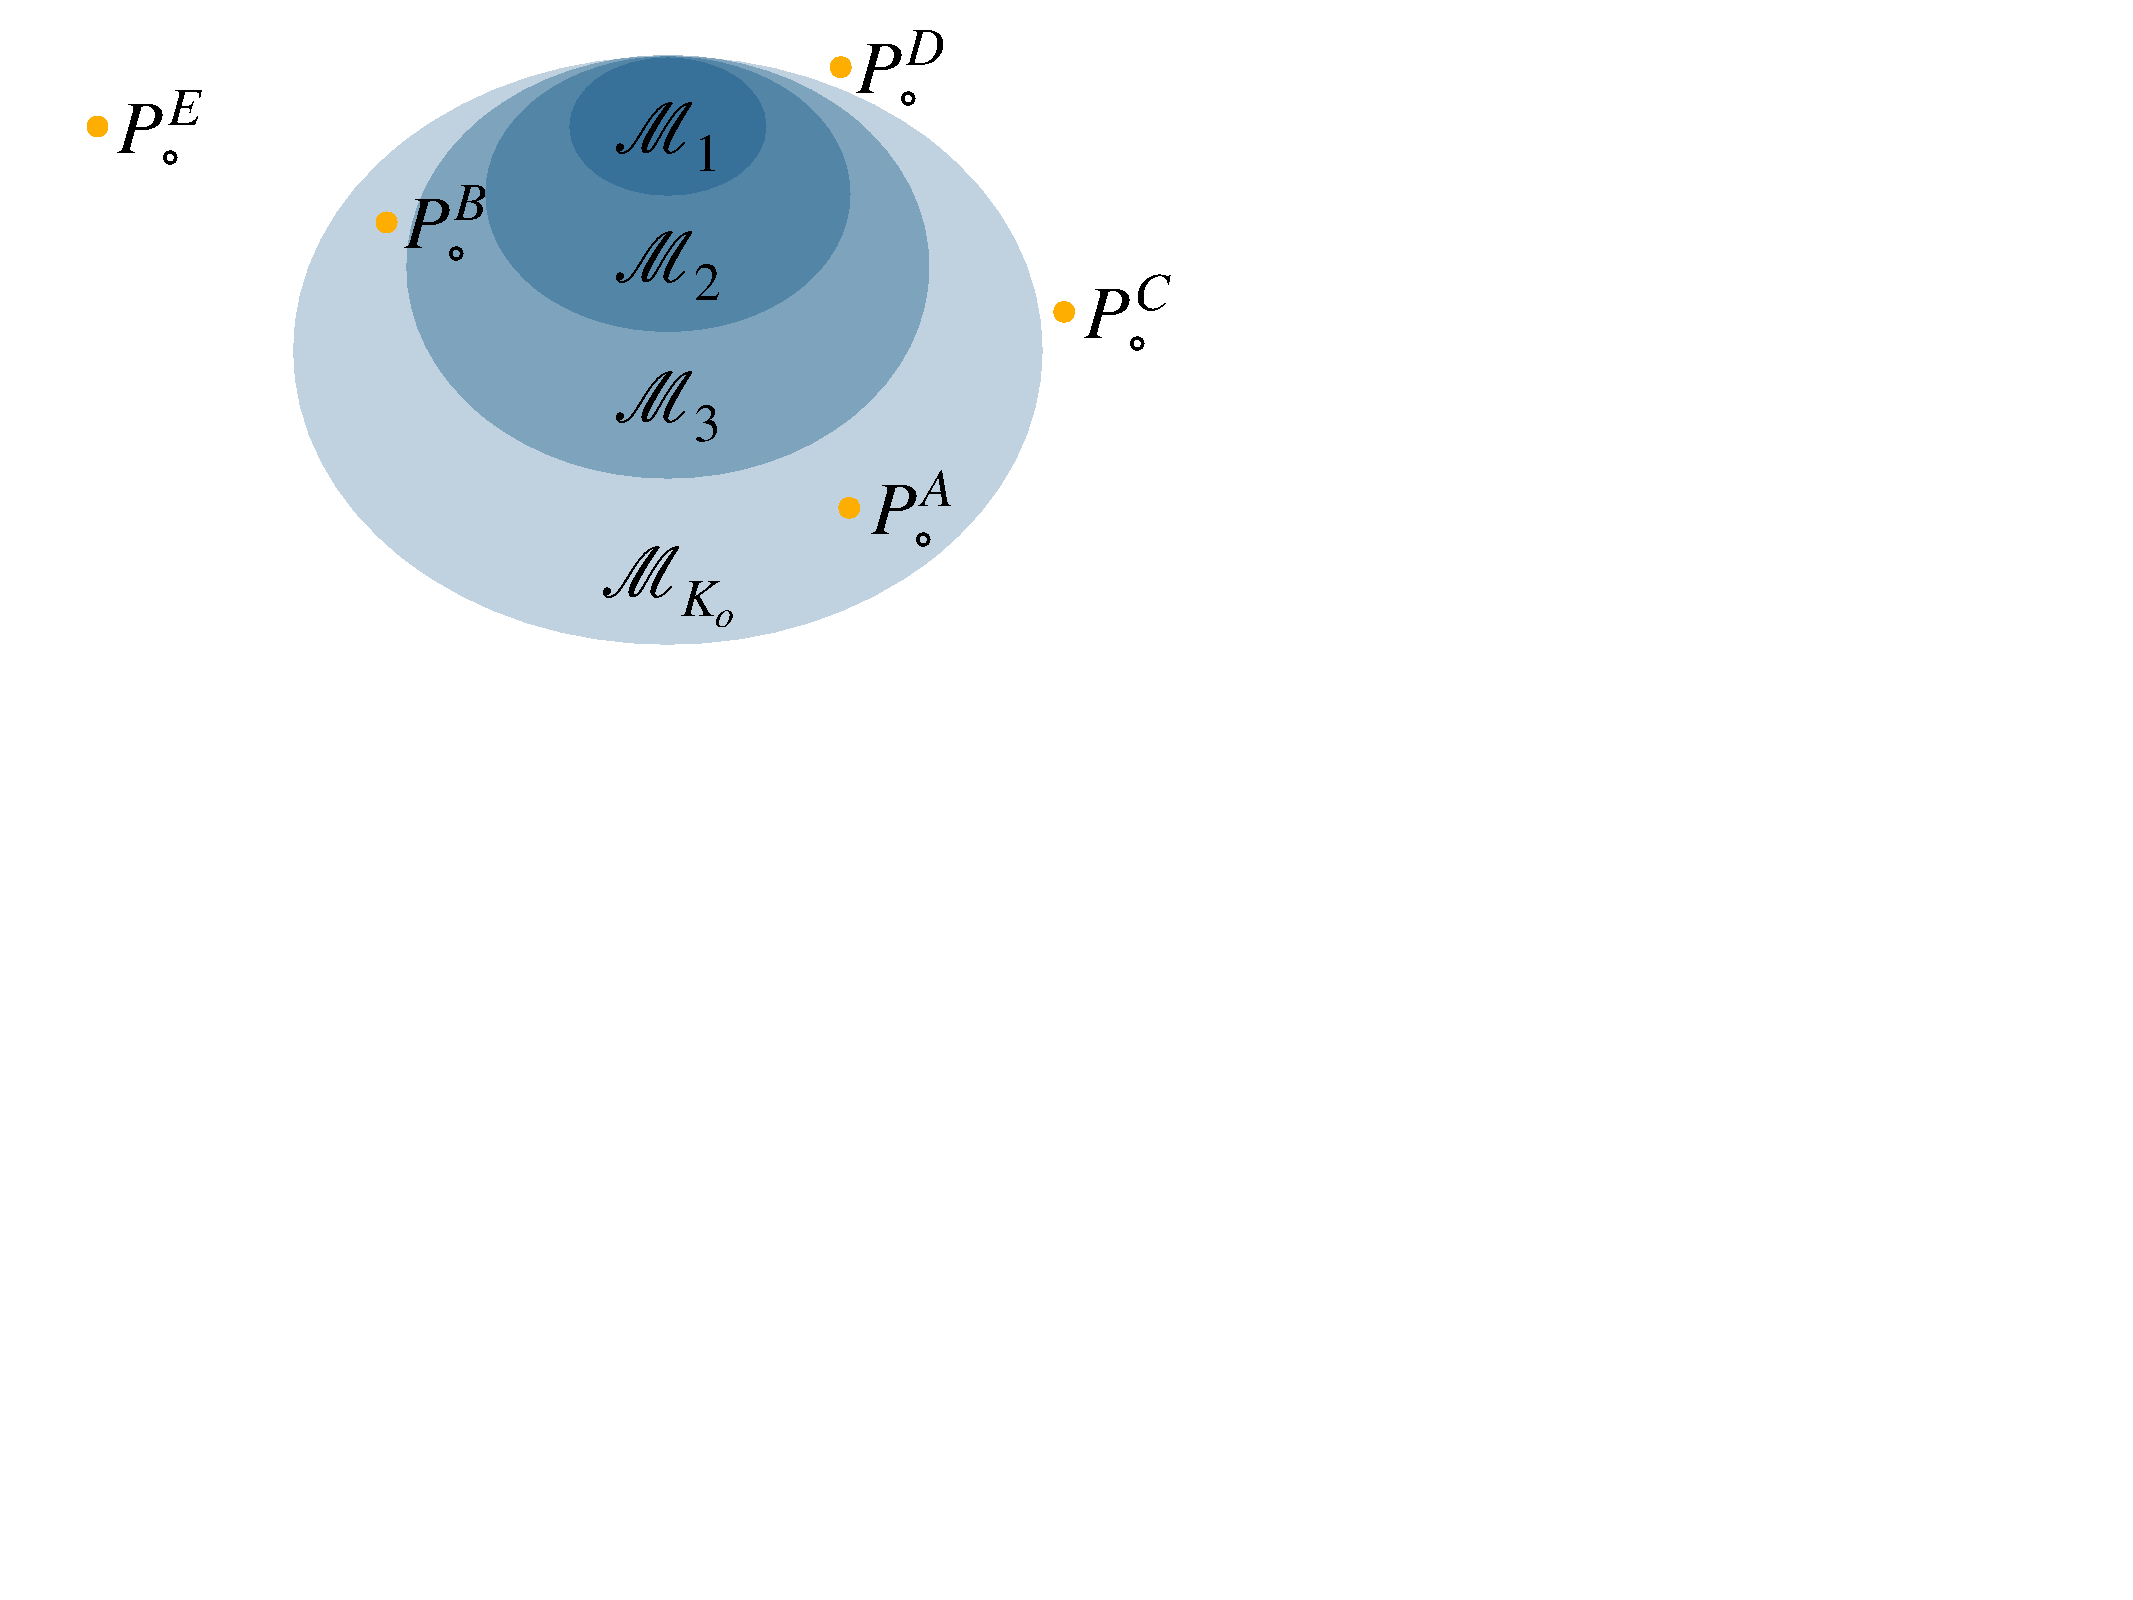
\includegraphics[width=.7\textwidth,trim=0in 6.2in 6.2in 0in,clip]{consistency-illustration}
	\caption{Cartoon illustration of the differences between traditional and robust model selection consistency
		where the true model corresponds to $K_{o} = 4$, with the nested models indicated by the gray ovals.
		We contrast five possible data-generating distributions, $P_{o}^{A}, \dots, P_{o}^{E}$, indicated by
		the gold points.
		Since $P_{o}^{A}, P_{o}^{B} \in \model{K_{o}}$ but are not in $\model{K}$ for $K < K_o = 4$,
		for these models $K_{o}$ can be consistently estimated.
		However,  since $P_{o}^{C}, P_{o}^{D}, P_{o}^{E} \notin \model{K_{o}}$, for these distributions
		$K_{o}$ cannot be estimated consistently in the traditional sense.
		On the other hand $P_{o}^{A}, P_{o}^{B}, P_{o}^{C}$, and $P_{o}^{D}$
		are close to $\model{K_{o}}$,
		so $K_{o}$ could potentially be robustly and consistently estimated in these four cases.
		However, $P_{o}^{B}$ and $P_{o}^{D}$ are also close to $\model{3}$, so robustly consistent
		estimation of $K_{o}$ is feasible only for $P_{o}^{A}$ and $P_{o}^{C}$.
		Since $P_{o}^{E}$ is far from $\model{K_{o}}$, $K_{o}$ would not be consistently estimable --
		either in the traditional or robust sense.
	}
	\label{fig:consistency-illustration}
\end{figure}



\subsection{A Plug-in Procedure}
\label{sec:method}

We propose a simple plug-in procedure for model selection, inspired by \cref{def:robust-consistency}.
Assuming $\rho_o = \rho(P_o, K_o)$ were known, we would want to find the smallest value of $K$ such that 
for all $k \in \{1,\dots,K\}$, we have $\compDisc^{(K)}(\theta_\star, k, P_{o}) \le \rho$ for $\theta_\star \in \Theta_{\star}^{(K_{o})}(P_{o})$.
However, since $P_{o}$ and $\Theta_{\star}^{(K_{o})}(P_{o})$ are unavailable, we propose to instead 
use the empirical distribution $\widehat{P}_o = \numobs^{-1} \sum_{n=1}^N \delta_{x_n}$, where $\delta_x$
is the Dirac measure at $x$, and a point estimator $\widehat\theta^{(K)}$.
Hence, we obtain the plug-in estimator $\compDiscEst^{(K,k)} = \compDisc^{(K)}(\widehat\theta^{(K)}, k, \widehat{P}_o)$.
Since values of $\compDiscEst^{(K,k)} < \rho_o$ are not important from a model selection perspective, 
we truncate the estimator by replacing it with $\max(0, \compDiscEst^{(K,k)} - \rho)$, where $\rho$ is 
a best estimate of $\rho_o$. 
We can view taking this maximum as serving a similar role to how the coarsened posterior conditions on the discrepancy having a known upper bound. 

Rather than taking the maximum over the component-wise discrepancy estimates, for better robustness
to noisy estimates we use a sum, which results in a robust model selection loss 
\[ \label{eq:robust-loss}
	\mathcal{R}^\rho(x_{1:n}, K) = \sum_{k=1}^K \max(0, \compDiscEst^{(K,k)} - \rho),
\]
where for notational simplicity we have left the dependence of $\compDiscEst^{(K,k)}$ on $x_{1:n}$ 
(as a function of $\widehat{P}_o$ and $\widehat\theta^{(K)}$) implicit. 
Since the loss is the sum (i.e., accumulation) of discrepancies that have been truncated (i.e., cut off) at $\rho$,
we call \cref{eq:robust-loss} the \emph{accumulated cutoff discrepancy criterion} (\methodname).
The corresponding robust model estimator is
\[
\widehat{K}^\rho(x_{1:n}) = \min\{\argmin_K \mathcal{R}^\rho(x_{1:n}, K)\}.
\]
Since $\argmin_{\numcomps}$ may return a set of values if the loss is equal to
zero for more than one value of $\numcomps$, it is necessary to include an
additional $\min$ operation to select the smallest value from the set.
We will discuss how to determine $\rho$ in \cref{sec:choosing-rho}. 

\subsection{Modeling Framework} \label{sec:framework}

\begin{figure}[tp]
	\centering
	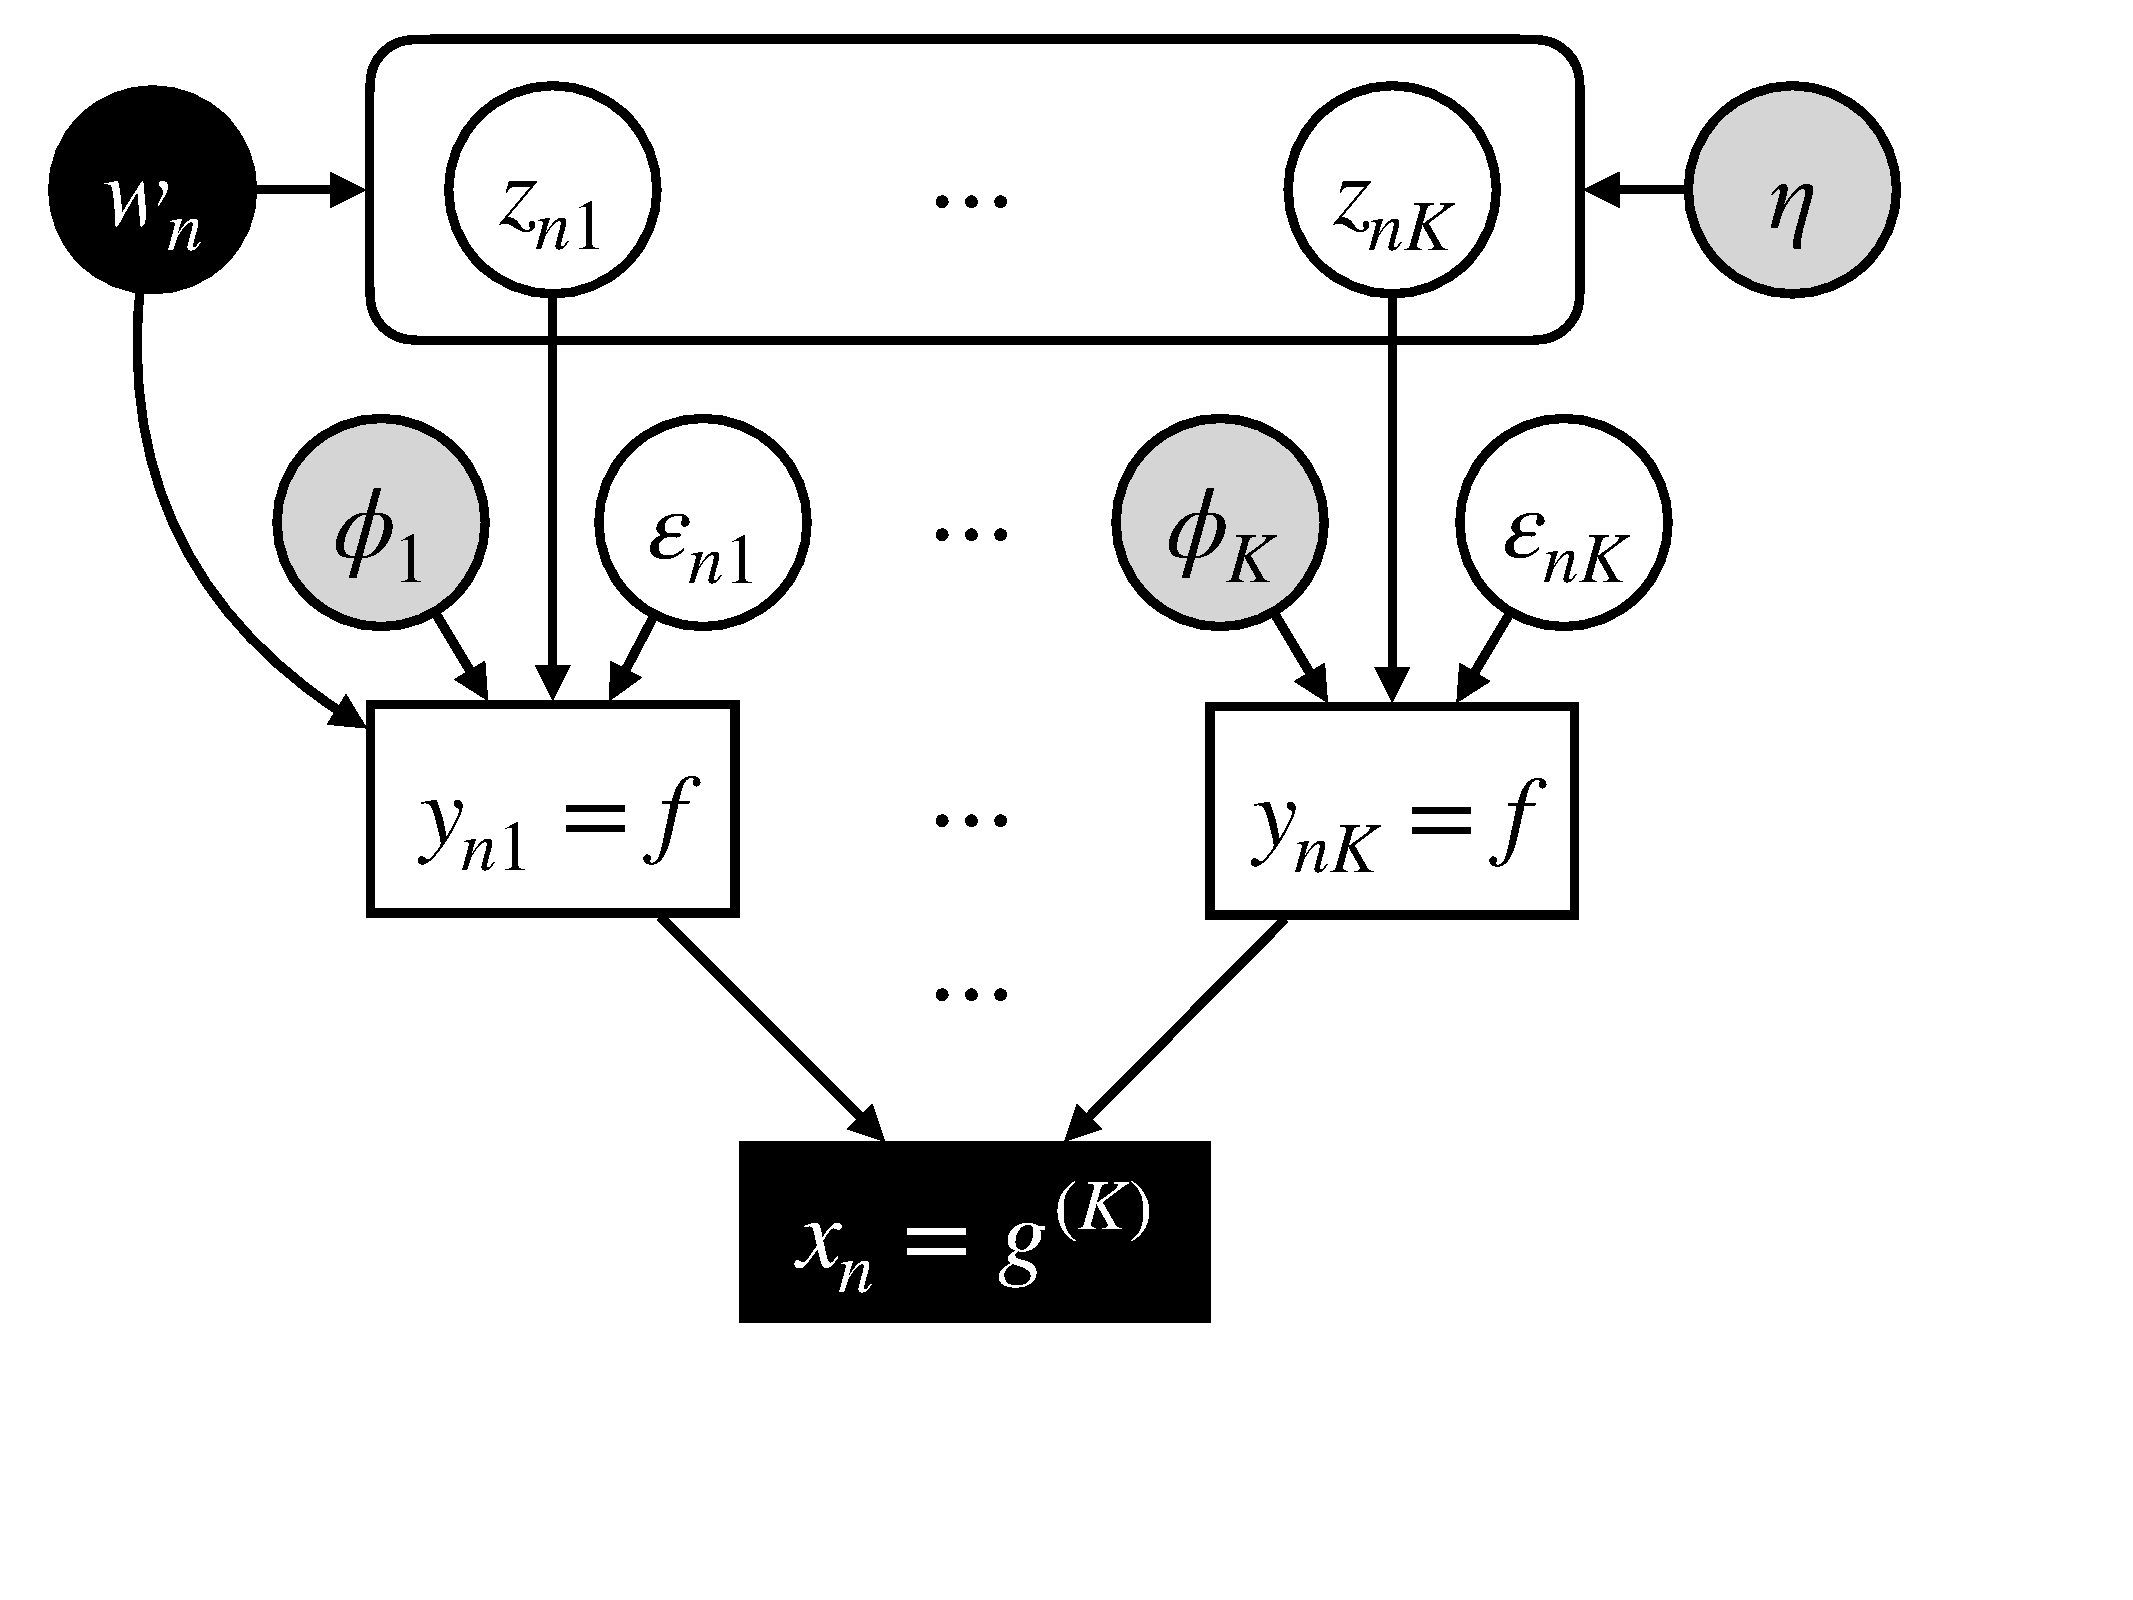
\includegraphics[width=.8\textwidth,trim=0in 1.9in 0in 0in,clip]{model}
	\caption{Graphical representation of the general form for model $\model{K}$ for a single observation $\data{n}$.
		Circles denote random variables while squares denote deterministic variables.
		A gray background indicates global parameters while a black background indicates an observed quantity.}
	\label{fig:model}
\end{figure}

Guaranteeing robust model consistency requires specific choices of model and component-level discrepancy.
In this paper, we consider a flexible modeling framework in which the observed data are the result of $K$ distinct latent sources (\cref{fig:model}). 
This framework will lead to a natural choice of component-level discrepancy, of which the mixture model
discrepancy proposed \cref{sec:robust-consistency} is a particular case. 

We allow each observation $x_n \in \mathcal{X}$ to have sample-specific covariates $w_n \in \mcW$.
Assume that $x_n$ depends on process-level contributions $y_{n1},\dots,y_{nK} \in \mathcal{Y}$ via the deterministic function $g^{(K)} \colon \mathcal{Y}^{\otimes K} \to \mathcal{X}$:
\[
	x_n = g^{(K)}(y_{n1}, \dots, y_{nK}).
\]
For example, we could have $g^{(K)}(y_1,\dots,y_K) = \sum_{k=1}^K y_k$ or $g^{(K)}(y_1,\dots,y_K) = \max_{k} y_{k}$.
The process-level contributions are in turn
determined by an observation-specific latent variable $z_n  = (z_{n1},\dots,z_{nK}) \in \mcZ^{(K)} \subseteq \mcZ^{\otimes K}$ and the process-specific parameters $\phi_1,\dots,\phi_\numcomps \in \Phi$.
We assume both $\mathcal{Y}$ and $\mcZ$ contain a \emph{null value} $\emptyset$, which indicates no contribution.
Specifically, we assume $g^{(K)}$ has the following \emph{no contribution property}: for all $y_1,\dots,y_{K-1} \in \mathcal{Y}$,
\[
	g^{(K)}(y_{1}, \dots, y_{K-1}, \emptyset) = g^{(K-1)}(y_{1}, \dots, y_{K-1}).
\]
Given a deterministic function
$f \colon \mcW \times \mcZ \times \Phi \times \reals \to \mathcal{Y}$
and independent noise random variables
$
	\varepsilon_{nk} \distiid G
$,
the component-level contributions are given by
\[
	y_{nk} = \begin{cases}
		\emptyset,                                  & \text{if $z_{nk} = \emptyset$,} \\
		f(w_{n}, z_{nk}, \phi_k, \varepsilon_{nk}), & \text{otherwise}.
	\end{cases}
\]
If there are no covariates, we drop the dependence on $w_n$ and write $f(z_{nk}, \phi_k, \varepsilon_{nk})$ instead.
Typically $\mcZ \subseteq \reals$ and $z_{nk}$ represents the activity level of the $k$th process for the $n$th observation.
In such cases, usually $\emptyset = 0$.
For a global parameter $\eta \in \mathcal{E}^{(K)}$, we assume the observation-specific latent variables are independent but may depend on the sample-specific covariates:
\[
	z_n \mid \eta, w_n \distiid H^{(K)}_{\eta,w_n}.
\]
If there are no covariates, we drop the dependence on $w_{n}$ and write $H^{(K)}_{\eta}$ instead.

Our framework captures many common model types: 

\begin{example}[Mixture Modeling]\label{ex:mix-model}
	We can recover a general mixture model by taking $H_\eta^{(\numcomps)} = \distCat(\eta)$, 
    %, where $\eta \in \Delta_{\numcomps} = \{ \eta \in \reals_{+}^{\numcomps} \mid \sum_{k=1}^{\numcomps} \eta_{k} = 1 \}$, the $(\numcomps-1)$-dimensional probability simplex.
	so $z_{nk} \in \{0,1\}$ and $\sum_{k=1}^K z_{nk} = 1$.
	Given a mixture component distribution family $\mcF = \{ F_{\phi} \mid \phi \in \Phi \}$,
	define $f$ such that, for  $\varepsilon \distas G$, it holds that
    $f(0, \phi, \varepsilon) = 0$ and $f(1, \phi, \varepsilon) \distas F_\phi$. 
	Finally, take $g^{(K)}$ to be the summation operator.
	Hence, if $z_{nk} = 1$, then $x_n = y_{nk} \distas F_{\phi_k}$.
\end{example}
\begin{example}[Mixture Model with Varying Component Probabilities] \label{ex:mix-model-varying}
	When covariates are available for each observation, the mixture model can be generalized to
	allow the mixture probabilities to depend on observed covariates \citep{Jaspers_BayesianEstimationMixtureCovariate_2018,Huang_MixtureRegressionModels_2012}.
	We can recover this model by using the same setup as \cref{ex:mix-model}
	but instead letting $H_{\eta,w_n}^{(\numcomps)} = \distCat(h(\eta, w_{n}))$ for some fixed function
	$h \colon \mcE^{(K)} \times \mcW \to \Delta_{\numcomps}$.
	% In particular, we have $z_{nk} \in \{0,1\}$
	% 	and $\sum_{k=1}^K z_{nk} = 1$.
	% 	Given a mixture component distribution family
	% 	$\mcF = \{ F_{\phi} \mid \phi \in \Phi \}$,
	% 	we can define $f$ such that $f(0, \phi, \varepsilon) = 0$ and $f(1, \phi, \varepsilon) \distas F_\phi$
	% 	if $\varepsilon \distas G$.
	% 	Finally, take $g^{(K)}$ to be the summation operator.
	% 	Hence, if $z_{nk} = 1$, then $x_n = y_{nk} \distas F_{\phi_k}$.
\end{example}
\begin{example}[Probabilistic Matrix Factorization]\label{ex:pmf-formulations}
	For probabilistic matrix factorization (PMF), $x_n \in \reals^{D}$.
	Let $\mcZ \subseteq \reals$ and $\Phi \subseteq \reals^{D}$.
	We assume that $\mcF = \{ F_{\mu} \mid \mu \in \reals^{D} \}$ is a location family of distributions satisfying $\int x F_\mu(\dee x) = \mu$ for all $\mu \in \reals^{D}$.
	Let $f$ satisfy $f(z, \phi, \varepsilon) \distas F_{z \phi}$ if  $\varepsilon \distas G$.
	For example, in nonnegative matrix factorization, $F_{\mu} = \Poiss(\mu)$ while in classical factor analysis $F_{\mu} = \Norm(\mu, \sigma^{2})$,
	where $\sigma^{2}$ can also be learned.
	Finally, take $g^{(K)}$ to be the summation operator.
\end{example}
It is similarly applicable to supervised variants of probabilistic matrix factorization models, functional clustering problems, and a variety
of other latent variable models \citep{Carvalho:2008,Chiou:2007,Cunningham:2014,West:2003,Blei:2007,Dunson:2000}.

To define the component-level discrepancy, it is tempting to directly apply the approach we took for mixture models
and quantify the difference between the distributions of $y_{n1},\dots,y_{nK}$ when $x_n \distas P_o$ and the modeled distributions of $y_{n1},\dots,y_{nK}$.
However, the distribution of $y_{nk}$ ($n=1,2,\dots$) may be different due to the sample-specific dependence on $w_n$ and $z_{nk}$.
To address this issue, we instead consider the discrepancy between the distribution of the noise variables $\varepsilon_{nk}$ when $x_n \distas P_o$ and the noise distribution $G$.
However, we must exclude $\varepsilon_{nk}$ if $y^{(K)}_{nk} = \emptyset$ because then it is no longer part of the graphical model (see \cref{fig:model}).
Dropping the dependence on $n$, the inferred distribution of the $k$th noise variable is
\[
\widetilde{G}_k^{(\theta)} = \int \mcL(\veps_{k} \mid y_k \ne \emptyset, x, w, \theta) P_o(\d x, \d w),
\]
where $\mcL(\veps_{k} \mid \cdots)$ denotes a conditional law of $\varepsilon_k$. 
Hence, define the discrepancy for the $k$th component by $\compDisc^{(K)}(\theta, k, P_o) = \discr{\widetilde G_k^{(\theta)}}{G}$.

To define an empirical version of $\compDisc^{(K)}(\theta, k, P_o)$, let
$\widehat G_{nk}^{(K)} = \mcL(\varepsilon_{nk} \mid x_n, w_n, \widehat\theta^{(K)})$, 
define the usage indicators $u_{nk}^{(K)} = \ind(y_{nk}^{(K)} \ne \emptyset)$, and denote the number of observations for component $k$ as $N_k^{(K)} = \sum_{n=1}^N u_{nk}^{(K)}$.
%If $\widehat G_{nk} = G$, then $\varepsilon_{nk}$ is unused, so define the usage indicators $u_{nk} = \ind(\widehat G_{nk} \ne G)$ and number of active observations for component $k$ as $N_k = \sum_{n=1}^N u_{nk}$.
Then the empirical distribution of the noise variables for component $k$ is
\[
	\widehat G_k^{(K)} = \frac{1}{N_k^{(K)}} \sum_{n=1}^N u_{nk}^{(K)} \widehat G_{nk}^{(K)}.
\]
Hence the estimated discrepancy for the $k$th component is given by $\compDiscEst^{(K,k)} = \discr{\widehat G_k^{(K)}}{G}$. 

In some scenarios, it is necessary to replace the divergence with an estimator because 
$\discr{\widehat G_k^{(K)}}{G}$ is undefined (e.g., the KL divergence) or not efficiently computable (e.g., the Wasserstein distance).
%However, if $\mcX$ is not discrete, the KL divergence becomes 
%more challenging to estimate because the empirical distribution $\widehat G_{k}$ is not absolutely continuous with respect to $G$.
In \cref{sec:kl-estimation}, we discuss how best to estimate the KL divergence in practice and provide supporting
consistency theory by modifying the two-sample KL divergence estimation theory developed in \citet{Wang:2009} to the one-sample estimation setting applicable to \methodname. 
In \cref{sec:case-study-details}, we discuss using the entropy-regularized Wasserstein distance (the Sinkhorn distance) 
as a stable, efficiently computable alternative to the Wasserstein distance that scales to high dimensions. 


\subsection{Choosing $\rho$} \label{sec:choosing-rho}

%While the results from \cref{sec:theory} show that, with an appropriate choice of $\rho$, our method consistently estimates the number of mixture model components,
%those results do not suggest a way to select $\rho$ in practice.
%In \cref{subsec:theory-rho-bounds}, we explored the theoretical bounds of selecting $\rho$. However, obtaining all the necessary information to compute the theoretical upper bound in a closed form is impractical in real-world applications. 
The value of $\rho$ is problem dependent, as it quantifies the maximum amount of model misspecification of each process.
We propose two complementary approaches to selecting $\rho$ that
take advantage of the fact that the robust loss is a piecewise linear function of $\rho$.
Therefore, given a fitted model for each candidate $\numcomps$, we can easily compute the loss for all values of $\rho$.

\paragraph{Using domain knowledge.}
The first approach aims to leverage domain knowledge. % to approximate its optimal value. 
Specifically, it is frequently the case that some related datasets are available with ``ground-truth'' labels either
through manual labeling or via \emph{in silico} mixing of data where group labels are directly observed \citep[see, e.g.,][]{Souto:2008}.
In such cases, an empirically optimal $\rho$ value %or range of candidate values
for one or more such datasets with ground-truth labels
can be determined by maximizing a problem-appropriate accuracy metric such as F-measure.
Because $\rho$ quantifies the divergence between the true process distributions and the model estimates,
we expect the values found using this approach will generalize to new datasets that are reasonably similar.
We illustrate this approach in \cref{sec:flow-cytometry}.
%This approach is employed in flow cytometry data, discussed in \cref{sec:experiments}.
%Data with available ground truths are frequently observed in cancer gene expression datasets, as illustrated in studies like .
%These ground truths are obtained through extensive manual labeling efforts.
%Leveraging the ground truth allows us to approximate the mismatch between the assumed model and the data, serving as crucial prior knowledge when determining appropriate $\rho$ values.
%Consequently, when confronted with new, unlabeled data for clustering, our model selection criterion shows robustness in handling known model misspecification. This robustness is a result of the prior understanding gained from the ground truth labels.

\paragraph{A general approach.}
For applications where there are no related datasets with ground-truth labels available, we
propose a second approach.  %This insight motivates our inference strategy. 
%Instead of pre-selecting $\rho$ or doing a grid search, we propose a two-step process.
After estimating the model parameters for each fixed $\numcomps$
and computing all process-wise divergences, we plot the loss as a function of $\rho$ for each $\numcomps \in \{\numcomps_{\min},\dots,\numcomps_{\max}\}$.
For readability, we introduce a small positive constant $\lambda \ll 1$ and plot $\mathcal{R}^{\rho}(\data{1:\numobs}, K) + \lambda \numcomps$
so it is possible to distinguish the lines when the loss is exactly zero.
The optimal model is determined by identifying the number of processes which is best over a substantial range of $\rho$ values,
with $\rho$ as small as possible.
The idea behind this selection rule is to identify the first instance of stability, indicating that allowing just a small amount of additional misspecification (by increasing $\rho$) doesn't notably improve the loss.
However, subsequent stable regions that appear afterward might introduce too much tolerance, potentially resulting in model underfitting.
This approach is similar in spirit to the one introduced for heuristically selecting the $\alpha$ parameter for the coarsened posterior \citep{Miller:2019}.


\begin{figure}[tp]
	\centering
	%	\subfloat{\includegraphics[width=.48\textwidth,height=40mm]{density-plot-true-K0=4}	\label{fig:stare-pois-den}}
	%\subfloat{\label{fig:sn-penloss-s1}	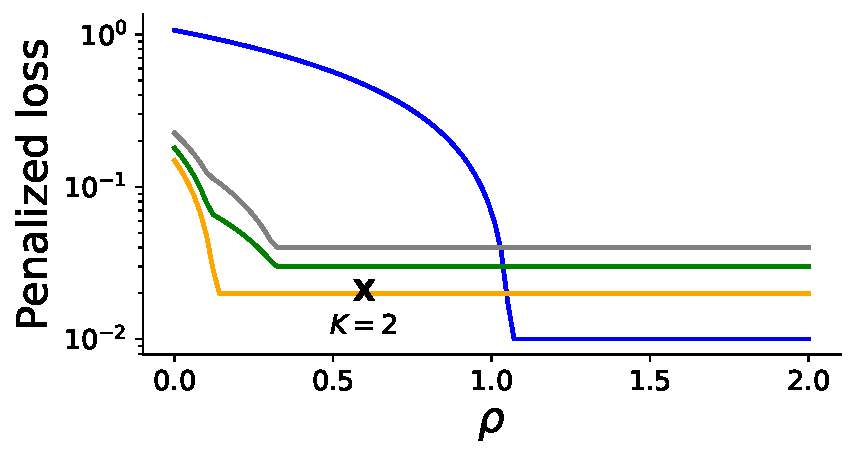
\includegraphics[width=.48\textwidth,height=40mm]{	skewnorm-stare-loss-n=5000-close-False-rsize-equal-rmis-equal}}
	%	\subfloat{\label{fig:sn-penloss-s2}	\includegraphics[width=.48\textwidth,height=40mm]{	skewnorm-stare-loss-n=5000-close-False-rsize-equal-rmis-bbig-small}}\\
	\subfloat{%\label{fig:poismm-penloss}	
		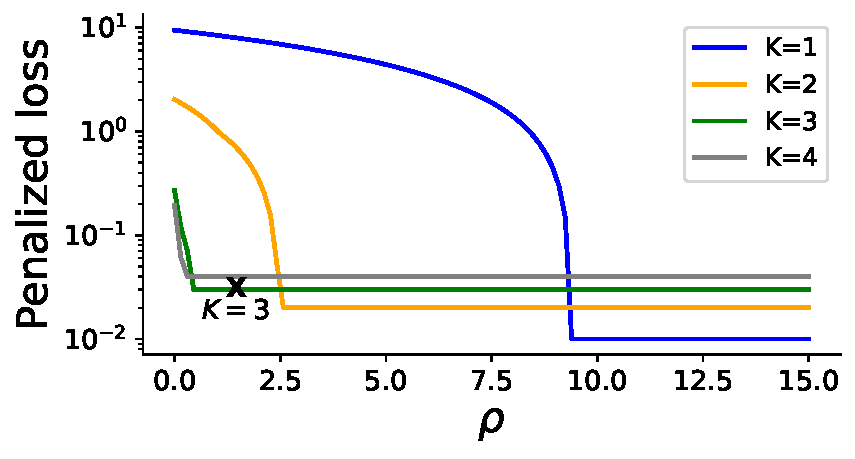
\includegraphics[width=.48\textwidth]{penloss-plot-N=20000-trueK=3-legend}}
	\subfloat{%\label{fig:poismm-fmeasure}	
		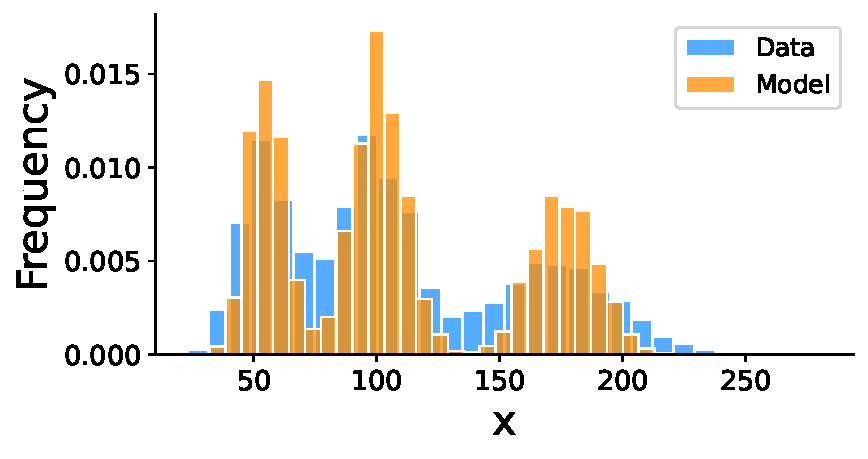
\includegraphics[width=.48\textwidth]{pois-hist-legend}}
	%	\caption{\PROBLEM{JL: Biometrika requires no legends.} The penalized structurally aware loss against $\rho$ for Scenario~(\ref{eg:s2}) (top left) and Scenario~(\ref{eg:s3}) (top right). For Poisson mixture models on data from negative binomial mixtures, penalized loss plot (bottom left) and component pmfs by our model selection compared to true distribution (bottom right).} 
	\caption{Fitting a Poisson mixture model to data from a mixture of negative binomial distributions (\cref{sec:choosing-rho}). \textbf{Left:} Penalized loss plot for $\numcomps \in \{1,2,3,4\}$. The cross mark indicates the first wide stable region and is labeled with the number of clusters \methodname selects. \textbf{Right:} Estimated model distribution compared to the observed data.}
	\label{fig:poismm}
\end{figure}

\begin{example}
    \PROBLEM{TODO: use Gaussian mixture example instead or remove completely}
	We illustrate our second approach using a Poisson mixture model simulation study.
	Suppose data $x_1, \ldots, x_{\numobs}$ is generated from a negative binomial mixture
	$P_o = \sum_{k=1}^{\numcomps_o} \eta_{ok}\distNBinom(m_k, p_k)$. %, where $\numcomps_o$ denotes the true number of clusters. 
	The assumed model is $G_{\theta} = \sum_{k=1}^{\numcomps} \eta_k \distPoiss(\param_k)$.
	We set $\numobs=20\,000, \numcomps_o = 3, m = (55, 75, 100), p = (0.5, 0.3, 0.5)$, and  $\eta_o = (0.3, 0.3, 0.4)$.
	We use the plug-in Kullback--Leibler estimator (see \cref{eq:plug-in-KL} in \cref{sec:kl-estimation}).
	%As \cref{thm:main} guarantees, structurally aware robust inference picks up the correct number of components with finite mixtures as data size is sufficiently large. 
	Based on \cref{fig:poismm}(left), the first wide and stable region corresponds to the true number of components $K = 3$.
	The observed data and fitted model distribution for $K = 3$ are shown in \cref{fig:poismm}(right).
\end{example}

\paragraph{Automation.}
Building on the same heuristic intuition, we can further automate the selection of $K$  by defining a minimum width $\Delta_{\min}$ for which an interval can be recognized as the stability region. Specifically,
% we define this stability interval by determining the range of $\rho$ over which the penalized loss for $K$ remains optimal. The lower bound is the first $\rho$ value where an $K$-specific loss first becomes the minimum among all losses, and the upper bound is the $\rho$ value where the loss is surpassed by the loss for a different $K$. By imposing a threshold on the length of such interval, we can automatically select the $K$ value corresponding to the first loss function satisfying this criterion.
we keep track of the smallest $\rho$ value, $\rho_\mathrm{start}$, for which a $K$-specific penalized loss becomes minimal among all other $K$-specific losses.
We then identify the next $\rho$ value, $\rho_\mathrm{end}$, at which this same loss curve is no longer the minimum.
The difference between $\Delta = \rho_\mathrm{end} - \rho_\mathrm{start}$ defines an interval of stability.
If $\Delta \ge \Delta_{\min}$ (i.e., $\Delta$ has the predefined minimum width), it is recognized as a stability interval, the corresponding value of $K$ is chosen to be $\widehat K$. Otherwise, $\rho_\mathrm{end}$ becomes $\rho_\mathrm{start}$
and repeat the procedure to compute the new $\rho_\mathrm{end}$ and $\Delta$, check if $\Delta \ge \Delta_{\min}$, and so forth.
The value of $\Delta_{\min}$ should be set based on preliminary manual experiments to estimate a suitable stability region width for automated selection in larger batches. This approach allows users to adjust the interval threshold to balance the tradeoff between avoiding underfitting ($\Delta_{\min}$ sufficiently small) and ensuring appropriately conservative and stable model selection ($\Delta_{\min}$ sufficiently large).
We demonstrate the utility of this approach in \cref{sec:case-study}. %, where it is applied to complex scRNA-seq data.

\subsection{Related Work} \label{sec:related-work}

\PROBLEM{TODO: update to focus on general-purpose methods; move discussion of model-specific methods to the applications section}
To address the overfitting problem in the misspecified setting, various robust methods have been developed for specific models.
For example, in the mixture model setting, heavy-tailed mixtures  \citep{Archambeau:2007,Christopher:2004,Wang:2018} and sample re-weighting \citep{Forero:2011}
both aim to account for slight model mismatches and outlier effects.
However, these methods do not directly address the question of how to choose the number of clusters for the mixture model beforehand.
%and their performance heavily relies knowing the number of subpopulations.
In the matrix factorization setting, \citet{Liu_Support-Union_2019} proposes a robust model selection method; however, it is limited to Gaussian nonnegative matrix factorization (NMF).
%, using the second-order moment from the empirical fourth-order cumulant tensor.
%However, the work had no mention of robustness against misspecification.
\citet{Pelizzola_NegBin-NMF_2023} aim to address the problem of robustness for the case of Poisson NMF using two different approaches: a negative binomial instead of a Poisson likelihood to improve the model's ability to handle overdispersed data, and a testing routine inspired by cross validation.
While this approach provides reasonable results, using the negative binomial only targets a very specific type of data--model mismatch, and the cross validation approach does not have any correctness guarantees.
\citet{Bai_DeterminingNumberFactors_2002} propose an information criterion based approach for factor analysis
and provide an asymptotic consistency result for the case where the input dimension tends towards infinity. However, the main result
applies only to the Gaussian NMF model with principle component analysis (PCA) as the estimation method.
Specific to the area of gene analysis, one common approach to selecting the number of signatures (K) is to evaluate the stability of the NMF solution across multiple runs. The cophenetic correlation coefficient method \citep{brunet_CCC_2004a} is one such example. A similar stability-based principle is adopted by the widely-used toolset SigProfilerExtractor \citep{islam_sigprofiler_extractor_2022}, which uses a consensus bootstrap approach to ensure results are consistent and reproducible. While this class of solutions is thorough, it can be computationally costly due to its reliance on repeated NMF executions. Furthermore, a recent study by \citet{Xue:2024} argues that this consensus bootstrap methodology may lead to a lack of robustness under model misspecification.
%Another significant limitation of the approaches just described is that they are limited to a specific model (e.g., mixture model or Poisson NMF), which limits modeling flexibility.
%Most closely related to our approach, 

There is limited work on general-purpose approaches to address overfitting.
Some recent work on robustifying likelihoods to small model perturbations \citep{Chakraborty:2023,Dewaskar:2023,Wu:2024} could provide a promising direction.
However, these methods cannot be used with existing parameter estimation methods -- which, as discussed above, is a key goal of the present work.
Additionally, \citet{Miller:2019} propose a conceptually simple robust Bayesian model selection
procedure by employing a technique they call \emph{coarsening}.
Unlike the standard posterior, which assumes the data were generated from the assumed model (that is, it conditions on $\data{} = \data{\mathrm{obs}}$), the \emph{coarsened posterior} conditions on the ``true model data'' being close to the observed data
(that is, it conditions on the estimated Kullback--Leibler divergence between $\data{}$ and $\data{\mathrm{obs}}$ being less than some threshold $\gamma$) -- hence, sacrificing predictive power for greater robustness.
%This flexibility permits the overall mixture model to deviate from the true underlying data by a set threshold.
%conditions on the event that the observed data are close to some ``idealized data'' that was generated from the assumed model. 
%\fTBD{Thinking about removing this sentence.}When such deviation is measured by relative entropy and an exponential prior is placed on the allowed deviation threshold, they show that the coarsened posterior is equal to the standard posterior to an appropriate power between zero and one. 
However, using the coarsened posterior approach has a potentially high computational cost because
it requires running Markov chain Monte Carlo dozens of times to heuristically determine a suitable robustness threshold \citep{Miller:2019,Xue:2024}.
Moreover, while coarsening offers good robustness in many scenarios, it does not have have any formal correctness guarantees
and can fail in simple situations.

\section{Applications}
\label{sec:experiments}

\PROBLEM{TODO: update intro to reflect changes in content }
We now demonstrate the practical utility of our robust model selection approach.
%h across a wide variety of applications using both mixture and probabilistic matrix factorization models. 
In each experiment, we compare to BIC since, like \methodname, it only requires a point estimate for each value of $K$.
Alternative criteria like AIC and DIC would give similar results.
However, note that BIC has a larger penalty than AIC (which DIC generalizes), so we choose BIC since it will be more conservative and hence tend to choose smaller values of $K$.
See, for example, \citet{Miller:2019,Xue:2024,Cai:2021} for numerical examples showing that Bayesian model selection does
not resolve the overfitting problem.
All experiments in this section we use the KL divergence as the discrepancy measure.
Mixture model experiments in this section and \cref{sec:case-study} use the EM algorithm to obtain parameter estimates.

\subsection{Mixture Models}

In \cref{sec:mixture-model-consistency}, we show that \methodname is robustly consistent for mixture models 
when the discrepancy measure is the KL divergence, Wasserstein distance, or maximum mean discrepancy.
\PROBLEM{TODO: discuss the required choices of gap function and $\distDisc$.}
\PROBLEM{TODO: describe alternative approaches that we will compare to.}
We compare ACDC against three mixture model selection criteria that rely on within-cluster dispersion. For $K$ clusters, the total within-cluster sum of squares is defined as
\[\mathrm{WCSS}(K) = \sum_{k=1}^{K} \sum_{i \in C_k} \| x_i - \mu_k \|^2,\]
where $x_i$ is the $i^{th}$ data point, $C_k$ is the set of points assigned to cluster $k$, and $\mu_k$ is its centroid. 
The Elbow method identifies the point beyond which additional clusters no longer show significant improvement in dispersion reduction. 
The Silhouette coefficient assesses how well each point fits within its assigned cluster relative to its distance to the nearest neighboring cluster \citep{siluet_coef}. It favors clusters with high cohesion where points are close to others in the same cluster, and high separation where clusters are well isolated from one another. 
The Gap statistic compares the observed clustering dispersion in the data to what is expected under a null reference where data comes from uniform distribution \citep{gap_stats}. The selection is based on the number of clusters that maximizes the deviation from its baseline. 

\subsubsection{High Dimensional Simulation Study}
\label{sec:high-dim-simulation}

We now provide further details about the motivating example in \cref{fig:motivate-comparison}, and illustrate
that \methodname selects the correct number of components under a variety of conditions on the level of misspecification,
the relative sizes of the mixture components, and the data dimension.
We generate data $x_1, \ldots,x_{\numobs} \in \reals^{D}$ from the mixture distribution
$P_{o} = \sum_{k=1}^{\numcomps_{o}}\eta_{ok}\distSNorm(m_{ok}, \Sigma_{ok}, \gamma_{ok})$,
where $\distSNorm(m, \Sigma, \gamma)$ denotes a skew normal distribution with location vector $m \in \reals^{D}$, scale matrix $\Sigma \in \reals^{D \times D}$,
and shape $\gamma \in \reals^{D}$, which controls the skewness.
The density of multivariate skew normal distribution is $f(x; m, \Sigma, \gamma) = 2\phi(x; m, \Sigma)\Phi(\gamma \odot x; m, \Sigma)$, where $\phi(x; m, \Sigma)$ and $\Phi(x; m, \Sigma)$ are, respectively, the probability density function
and cumulative distribution function of the multivariate normal $\distNorm(m, \Sigma)$.
When $D > 1$, we introduce weak correlations by letting $\Sigma_{ok} = \Sigma$,
where $\Sigma_{ij}=\exp\{-(i-j)^2/\sigma^2\}$ and $\sigma$ controls the strength of the correlation.

When $D = 1$, our results confirm that \methodname robustly recovers the correct number of components.
Full details can be found in \cref{sec:simulation-gauss}.
As discussed in \cref{sec:kl-estimation}, the KL divergence $k$-nearest-neighbor estimator becomes less accurate with increasing data dimension.
While a general solution is unlikely to exist, we illustrate one approach to address this challenge.
Specifically, if we believe the coordinates are likely to be only weakly correlated, we can employ the $k$-nearest-neighbor
method on each coordinate by assuming the coordinates are independent.
For this higher-dimensional illustration, we set $D = 25$, $N=10\,000$, $K_{o}=3$, and $\sigma=0.6$.
As shown in \cref{fig:high-dim}(left), the wide and stable region corresponds to the true correct number of components.
\cref{fig:high-dim}(right) illustrates the value of model-based clustering, particularly in high dimensions: 2-dimensional
projections of the data give the appearance of there being four clusters in total, when in fact there are only three.

%to further explore the applicability of \methodname in high-dimensional cases.
\begin{figure}[tp]
	\centering
	\subfloat{\label{fig:high-dim-stare-loss}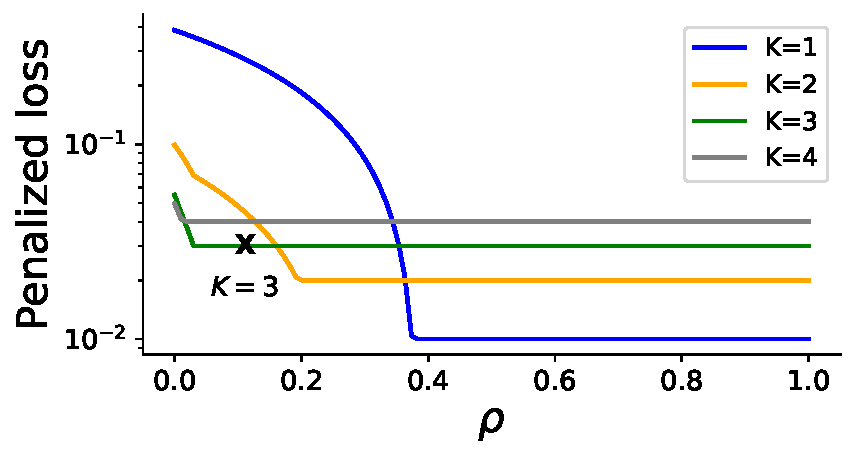
\includegraphics[width=.48\textwidth]{multiGMM-penloss-rho-n=10000-d=50-legend}}
	\subfloat{\label{fig:high-dim-true}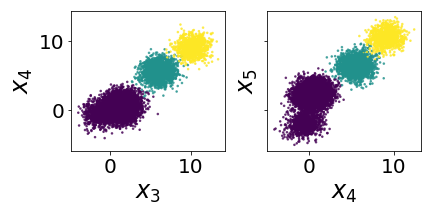
\includegraphics[width=.48\textwidth]{selected-cluster-plot-comparison-K=3}}

	\caption{Application of \methodname clustering simulated high dimensional data (\cref{sec:high-dim-simulation}).
		\textbf{Left:} The penalized loss plot for $\numcomps \in \{1,2,3,4\}$.
		Since the loss for $K=3$ is very close to equal to or much less than the loss for $K \ne 3$, it shows the greatest
		stability, resulting in $\widehat K = 3$ (indicated by the ``$X$'').
		\textbf{Right:} Selected two-dimensional projections of the data.}
	\label{fig:high-dim}
\end{figure}





\subsubsection{Cell Type Discovery using Flow Cytometry}
\label{sec:flow-cytometry}

Flow cytometry is a technique used to analyze properties of individual cells in a biological material.
Typically, flow cytometry data measures 3--20 properties of tens of thousands cells.
Cells from distinct populations tend to fall into clusters and discovering cell types by identifying clusters
is of primary interest in practice.
Usually scientists identify clusters manually, which is labor-intensive and subjective.
Therefore, clustering methods that provide interpretable groups of cells is invaluable.
We follow the setup of \citet{Miller:2019} using 12 flow cytometry datasets originally from a longitudinal study of graft-versus-host disease %(GvHD) 
in patients undergoing blood or marrow transplantation \citep{Brinkman:2007}.
Manual cluster assignments of all dataset are treated as the ground truth.
%the manual clustering is available and we take it as the ground truth. % to measure the performance of \methodname.
The datasets consist of $D=4$ dimensions and varying number of observations for each dataset.
%We set the scale as $k = \numobs^{1/2}$ in the adaptive $k$-nearest-neighbor based Kullback--Leibler estimator, which shows superior performance when $D= 4$.

We follow \citet{Miller:2019} and use F-measure to quantify clustering accuracy and calibrate $\rho$ using the first 6 datasets.
%For these datasets, we  %and then use this value $\rho$ for model selection for the other 6 datasets. 
%More precisely, we find the $\rho$ value maximizes the average F-measure across the first 6 datasets.
As shown in \cref{fig:flowcyt-train}, the training datasets 1--6 have a nearly identical trend of
clustering accuracy as a function of $\rho$.
The averaged F-measure achieves the maximum when $\rho \approx 1.16$, which is a point of maximum F-measure for all 6 datasets.
The consistency of \methodname compares favorably to using coarsening, where drastically different $\alpha$ values maximize the F-measure \citep[Figure 5]{Miller:2019}.
These results provide evidence that our approach is taking better advantage of the common structure and degree of misspecification across datasets.

\begin{figure}[tp]
	\centering
	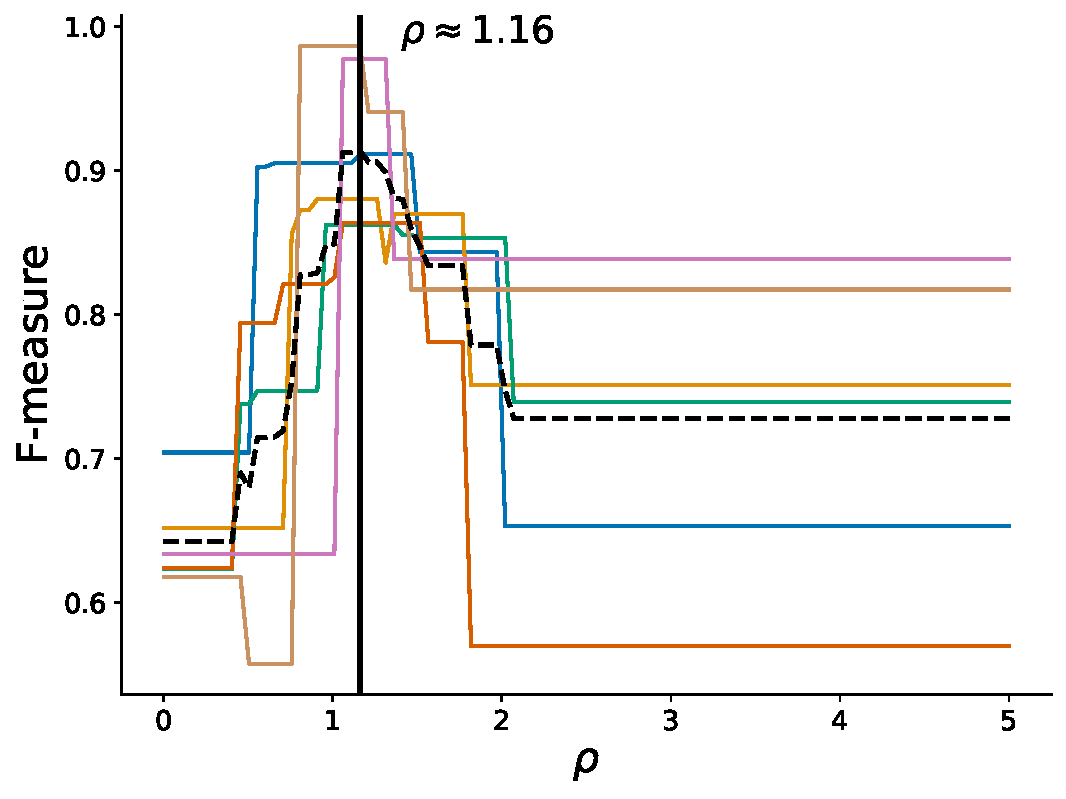
\includegraphics[width=80mm]{GvHD-train}
	\caption{Selecting an optimal value of $\rho$ using the first 6 flow cytometry datasets (\cref{sec:flow-cytometry}).
		The solid lines show $\rho$ vs.\ F-measure for datasets 1--6.
		The black dashed line indicates averaged F-measure over the training datasets.
		The vertical black line shows the value $\rho = 1.16$ that maximizes the averaged F-measure.}
	\label{fig:flowcyt-train}
\end{figure}


\begin{table}[tp]
	\centering
	\def~{\hphantom{0}}
	% 	\tbl{F-measures on flow cytometry test datasets 7--12}{
	\caption{F-measures on flow cytometry test datasets 7--12} {
		\begin{tabular}{ccccccc}
			\hline
			                                                   & 7             & 8             & 9             & 10            & 11            & 12            \\ \hline
			Structurally aware                                 & 0.63          & \textbf{0.92} & \textbf{0.94} & \textbf{0.99} & \textbf{0.99} & \textbf{0.98} \\ \hline
			\begin{tabular}[c]{@{}c@{}}Coarsened \end{tabular} & \textbf{0.67} & 0.88          & \textbf{0.93} & \textbf{0.99} & \textbf{0.99} & \textbf{0.99} \\ \hline
		\end{tabular}}
	\label{tab:flowcyto-test}
\end{table}

%
%\begin{figure}[tp]
%	\begin{minipage}{0.48\textwidth}
%		\centering	
%	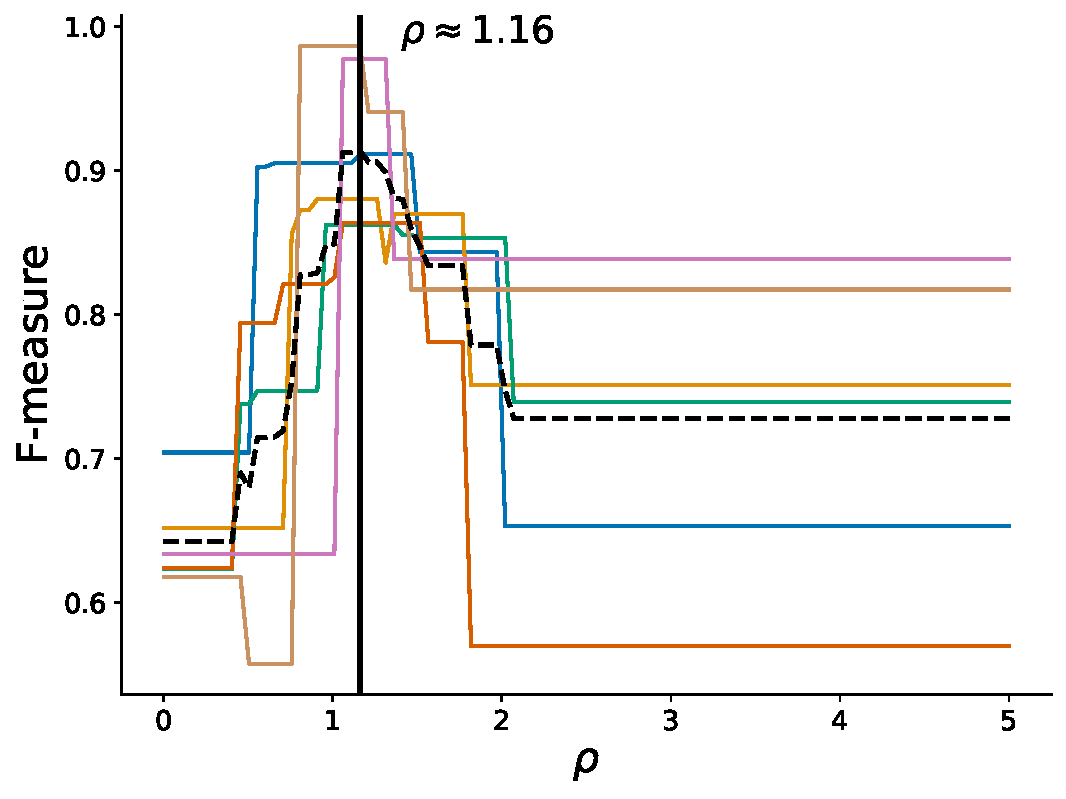
\includegraphics[width=.48\textwidth]{GvHD-train}
%	\end{minipage}\hfill
%	\begin{minipage}{0.48\textwidth}
%	\caption*{Table 1: F-measures on flow cytometry test datasets 7-12.}
%		\label{tab:flowcyto-test}
%		\begin{tabular}{ccc}
%			\hline
%			Dataset & Structurally aware   & Coarsened \\ 
%			\hline
%			7     & 0.63    & \textbf{0.67}      \\ 
%			8       & \textbf{0.92} & 0.88       \\ 
%			9        & \textbf{0.94}    & \textbf{0.93}   \\
%			10       & \textbf{0.99}  & \textbf{0.99}    \\ 
%			11       & \textbf{0.99}  & \textbf{0.99}     \\ 
%			12        & \textbf{0.98}    & \textbf{0.99}   \\ \hline
%	\end{tabular}
%	\end{minipage}
% \caption{F-measure against $\rho$ for training datasets 1-6. The black dashed line indicates averaged F-measure over the training datasets. Solid lines correspond to datasets 1-6.}
%	\label{fig:flowcyt-train}
%\end{figure}



%To determine the misspecification level $\rho$, we run structurally aware robust selection on the first 6 datasets.
%We aim to pick up $\rho$ such that the F-measure attains the maximum on the overall 6 training datasets.
%The clustering performance is measured by comparing the assignment to the ground truth and computing the F-scores accordingly.
%For each $\rho$, select $\numcomps$ that achieves the minimum penalized loss and then we can use the associated parameters to compute the F-measure.

For test datasets 7--12, we pick the value of $\numcomps$ based on a value of $\rho$ that is as close as possible to the estimated $\rho$ value of $1.16$ while also being stable for a range of $\rho$ values.
As shown in \cref{tab:flowcyto-test}, \methodname provides the same average accuracy as the coarsened posterior
while being substantially more computationally efficient, despite using a much slower programming language for implementation (2 hours using Python versus 30 hours using Julia). % rounded 1.9 and 30.4
%However, it takes approximately $30$ min to obtain similar clustering accuracy on the test datasets as coarsened posterior shows while running coarsened posterior takes $2.5$ hours which is significantly longer than structurally aware robust inference procedure.


%Set  $\rho = 1.16$ and run structurally aware robust selection on the remaining flow cytometry datasets 7-12. 



%\subsection{Single-cell RNA mosquito data}
%\label{sec:scRNA}
%
%The RNA expression data for olfactory receptors in mosquito neurons is stored as binary signals. 
%Assume data $X\in R^{M\times N}$ and $X_{ij} = 1$ indicates that the receptor $j$ is expressed in neuron $i$, for $i=1,\ldots,M$ and $j=1,\ldots,N$ and $X_{ij} = 0$ vice versa.
%In practice, some receptors show similar expression on several types of neurons and therefore a clustering method is often utilized to learn the structure and similarities between receptors and neurons.
%However, the unknown total number of types makes the problem challenging. 
%
%To better understand the performance of our method, we first apply our model selection rule with a synthetic cell-type model. 
%The generative model assumes that in one model, each receptor $X_i$ has a uniform probability of expression $\alpha_j$, and is expressed in each neuron independently and with identical distributions. 
%
%
%We test our model selection method in this case to pick up a model of receptor expression.
%As shown in \cref{fig:scRNA}, our method picks up the true underlying number of types $\numcomps=3$ and it shows consistency with the F-measure plot.
%
%
%
%\begin{figure}[tp]
%	\centering	
%	\subfloat{\includegraphics[height=40mm,width=.48\textwidth]{mosquito-loss-plot-Kt=3-M=10000-N=10}}
%	\subfloat{\includegraphics[height=40mm,width=.48\textwidth]{mosquito-fmeasure-plot-Kt=3-M=10000-N=10}}
%	
%	\caption{Left: penalized structurally aware loss against $\rho$; Right: F-measure against $\numcomps$ for simulated single-cell RNA mosquito data.} 
%	\label{fig:scRNA}
%\end{figure}
%

\begin{figure}[h!]
	\centering
	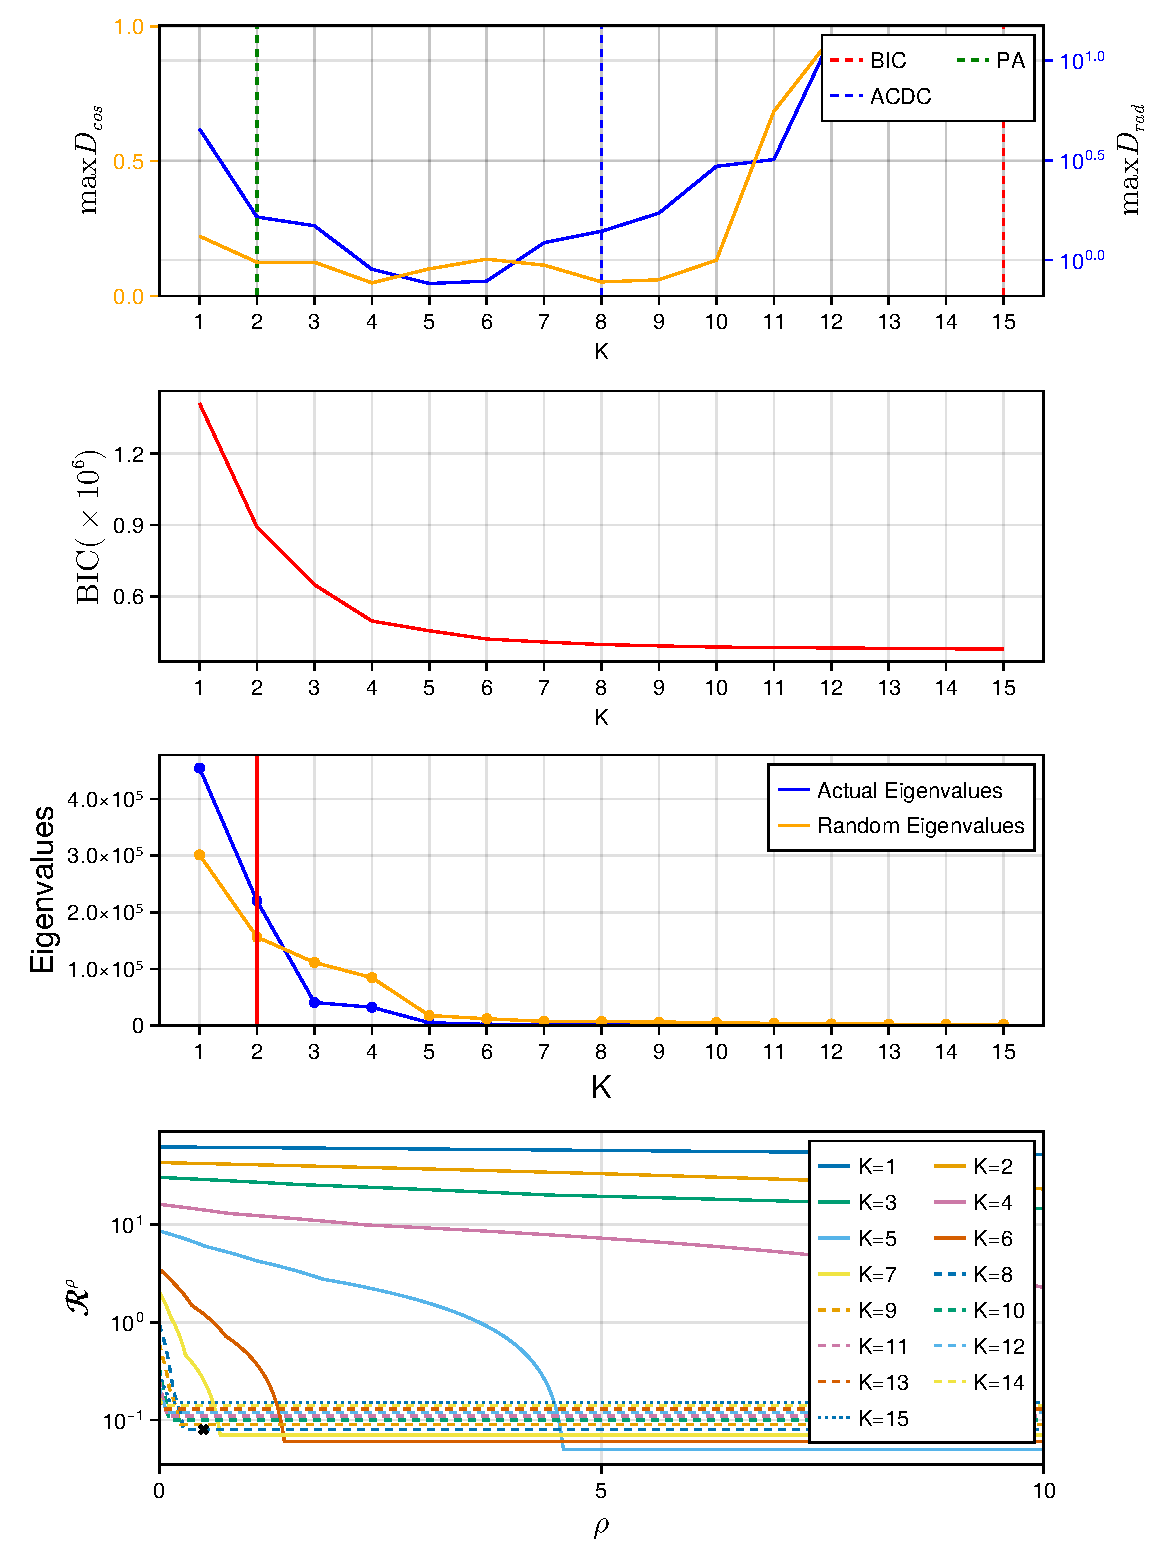
\includegraphics[width=.8\textwidth]{figures/composite-multdiv-600-breast-custom-seed-1-perturbed-0.0025.pdf}
	\caption{
	Estimation quality of mutational signature discovery for
	perturbed synthetic breast cancer data (\cref{sec:mutsigs}).
	\textbf{(top)} Errors of signature and loadings estimates.
	\textbf{(middle top)} $K$ versus value of BIC. BIC selects $\widehat K=K_{\max}$.
	\textbf{(middle bottom)} Scree plot generated from the dataset, indicating that $K = 2$ is the optimal choice of $K$.
	\textbf{(bottom)} Structurally aware loss for $K\in \{1,\dots,K\}$, the wide region with the smallest $\rho$ is marked by the cross mark, indicating $K=7$ or $K=8$ is the most appropriate choice of $K$.
	}
	\label{fig:mutsig_result}
\end{figure}

\subsection{Probabilistic Matrix Factorization} \label{sec:pmf-applications}

In \cref{sec:PMF-consistency-proof}, we show that \methodname is robustly consistent for probabilistic matrix factorization models 
when the discrepancy measure is the KL divergence.
\PROBLEM{TODO: discuss the required choices of gap function and $\distDisc$.}

For our applications, we take $G = \Unif([0,1]^{D})$, the uniform distribution on the $D$-dimensional hypercube.
This choice is without loss of generality when using KL divergence as the discrepancy measure since it is invariant to diffeomorphisms of the noise variables ${\veps}_{nk}$.
Moreover, it leads to a universal choice of $f(z, \phi, \cdot) = F^{-1}_{z\phi}$, the inverse CDF.
However, in specific scenarios other $G$ and $f$ might be preferred due to considerations such as ease of implementation or because
estimation of the KL divergence is more stable.
For example, in the Gaussian case, we could take $G = \Norm({0}, I)$ and $f(z, \phi, \veps) = z\phi + \sigma \veps$. 

We will be comparing \methodname against the Bayesian Information Criterion (BIC) and Parallel Analysis (PA), both very commonly used method for model selection in NMF and FA scenarios. BIC is computed by
\[
BIC\left(x_{1:N},z^{(K)}_{1:K,1:N},\phi^{(K)}_{1:K}\right) = K\log(N) - 2\log\left(p\left(x_{1:N}~\middle|~ z^{(K)}_{1:K,1:N},\phi^{(K)}_{1:K}\right)\right)+2\log(K!).
\]
And PA is carried out by generating the scree plot (PCA eigenvalues) of the data against that of randomly generated matrices of the same size. These random matrices are generated by independently permuting each row of the data matrix.

\subsubsection{Mutational Process Discovery} \label{sec:mutsigs}

Exposure to, and presence of, carcinogenic processes such as UV radiation, tobacco smoke, defective DNA repair mechanisms, and naturally occurring biochemical reactions, generate characteristic patterns of somatic mutations known as \emph{mutational signatures} \citep{Alexandrov_mut-sig-NMF_2013,Nik-zainal_MutationalProcessesMolding_2012}.
%as well as the mutational load due to each signature in each tumor sample. 
Mutational signature-based analyses have contributed to novel insights in cancer research \citep[e.g.,][]{Alexandrov_mut-sig-NMF_2013,Nik-zainal_MutationalProcessesMolding_2012,pcawgSV:2020,pcawg2020} and are leading to emerging translations in clinical settings \citep[e.g.,][]{Chakravarty:2021}.
The most widely used approach to signature discovery is to fit a Poisson non-negative matrix factorization (NMF) model. % have proven effective in discovering mutational signatures.
% The analysis of mutational signatures from tumor genome sequencing data (e.g., mutational count matrices) can yield information about a cancer's mutational mechanisms.
% This is important since there is growing interest in using the information to help diagnosis, prognosis and therapeutics.
%\subsubsection{Reverse sampling for Poisson PMF}
% In mutational signature discovery, a Poisson nonnegative matrix factorization (NMF) model is typically used \citep{Alexandrov_mut-sig-NMF_2013,Nik-zainal_MutationalProcessesMolding_2012}\PROBLEM{TODO(JHH): add whatever citations we use in \citep{Xue:2024} to support the choice of NMF}.
%In the Poisson NMF model, 
For each of $N$ tumor sample, the data consist of a count vector ${x}_{n}\in\nats^{D}$,
where $D$ is the number of mutation types being considered (e.g., there are $D=96$ single-base substitution types with a trinucleotide context).
% \[\label{eq:Pois_PMF}    
%   {y}^{(K)}_{n,k}&\mop{\sim}^{\mathrm{e.w}}\mathrm{Pois}\lrp{{\phi}^{(K)}_{k}z^{(K)}_{n,k}} \quad 
%   &&\text{for}\ n\in1:N,k\in1:K\\
%   {x}_{n}&=\sum^{K}_{k=1}{y}^{(K)}_{n,k}\quad&&\text{for}\ n\in1:N,
% \]
%where $\mop{\sim}\limits^{\mathrm{e.w}}$ means the distributional relation applies independently element-wise, ${x}_{n}\in\nats^{D}$ are vectors containing the counts of each type of mutation, ${\phi}^{(K)}_{k} \in\Delta_{D}$ denotes the $k$th mutational signatures, which is restricted to the $(D-1)$-dimensional probability simplex, and $z^{(K)}_{n,k}\in\reals_{+}$ indicates the amount of exposure of the  $n$th sample to the $k$ mutational process, which is represented by the signature ${\phi}^{(K)}_{k}$. 
The number of mutations of type $d$ in sample $n$ due to mutational process $k$ is given by
$y^{(K)}_{nkd} \sim \Poiss({\phi}^{(K)}_{kd}z^{(K)}_{nk})$ and hence the total number of mutations of type $d$ in sample $n$ is $x_{nd} = \sum_{k=1}^K y^{(K)}_{nkd}$.

% Applying Bayes' rule on formulation \eqref{eq:stare_formula}, we can sample ${\veps}_{n,k}\mid{x}_{n}$ for any given $n,k$.
% This sampling process can be used to construct an approximation to $\widehat{G}^{(K)}_{k}$.
%\subsubsection{Synthetic breast cancer dataset}
Because it is nearly impossible to obtain ground-truth signatures for real data, we use
simulated breast cancer data
%This experiment is performed on simulated data generated 
based on the COSMIC v2 catalog and the pan-cancer analysis of whole genomes (PCAWG),
following the procedure of \citet{Xue:2024}.
First, we applied nonnegative least squares regression to the count matrix and COSMIC signatures, resulting in best fit exposure vectors.
We then selected the signatures with significant loadings contributions and used them as the ground-truth signatures ${\phi}_{o}$, with
the inferred per-sample loadings serving as the ground truth exposures,
$z_{o 1}, \dots, z_{o N}$.
%is generated by perturbing the average of the exposure vectors.
Finally, we generated four synthetic datasets: one well specified, and three others each with a different form of model misspecification.
The forms of misspecification we use are from \citet{Xue:2024}:
\begin{itemize}
	\item \textbf{Perturbation:} for each ${x}_{n}$, the signatures ${\phi}_{o}$ are stochastically perturbed
	      before being used to simulate the observed counts.
	\item \textbf{Contamination:} for each ${x}_{n}$, in addition to the ground truth signatures ${\phi}_{o}$,
	      a randomly generated signature with small exposure is included in the sampling process.
	\item \textbf{Overdispersion:} the data is sampled from a negative binomial distribution instead of a Poisson distribution.
\end{itemize}

For each value of $K$, we compute the MLE of the signature and loadings parameters using the multiplicative update algorithm %with the divergence loss 
\citep{Lee-Seung_multdiv_2000}.
%To quantify the difference between the estimate and the ground truth.
As is standard practice, we quantify the signature recovery error using the cosine difference $
	D_{\mathrm{cos}}({\phi},{\phi}_{\star})=1-\langle {\widetilde\phi},{\widetilde\phi}_{\star} \rangle$, where for any vector ${v}$, we define ${\widetilde v} = {v} / \norm{{v}}_{2}$.
%$, which is $1\ -$ the cosine similarity.
For the exposures, we quantify the error using the relative average difference
$
	D_{\mathrm{rad}}({z}, {z}_{\star})= {\abs{\overline{z}-\overline{z}_{\star}}}/{\overline{z}_{\star}},
$
where for a vector ${v} \in \reals^N$, $\overline{v} = N^{-1}\sum_{n=1}^N v_n$.
To evaluate the quality of an estimate as a whole, we perform bipartite matching against the ground truth by minimizing the metric
\[
	D^{(K)}(\sigma)=\sum^{K}_{k=1}\lrb{D_{\mathrm{cos}}\lrp{{\phi}^{(K)}_{k},{\phi}_{o\sigma(k)}}
		+0.1\, \tanh\, D_{\mathrm{rad}}\lrp{{z}^{(K)}_{k},{z}_{o\sigma(k)}}},
\]
where $\sigma \colon [K_o] \to [K]$ denotes an injective matching function.
Given the optimal matching $\sigma_{\star} = \argmin_\sigma D^{(K)}(\sigma)$, the accuracy scores are defined
as the worst-case cosine and relative average errors, given by
$
	L^{(K)}_{{\phi}} = \max\{D_{\mathrm{cos}}({\phi}^{(K)}_{k},{\phi}_{o\sigma_{\star}(k)}) : k=1,\dots,K \},
$
and
$
	L^{(K)}_{z} = \max\{D_{\mathrm{rad}}(\overline{z}^{(K)}_{k},\overline{z}_{o\sigma_{\star}(k)}) :  k=1,\dots,K\}.
$

\Cref{fig:mutsig_result,fig:mutsig_result_appendix_1} show that, across all four datasets,
BIC selects $\widehat{K} = K_{\max}$ -- even when the data is well specified.
On the opposite spectrum, PA consistently underestimatess the number of signatures at $K = 2$. Finally, \methodname selects $\widehat K = 7$ or $8$, which correspond to the some of the largest values of $K$ for which the parameter estimates still have reasonably small error and meaningful decomposition.
These results suggest \methodname is a promising alternative to existing approaches for selecting the number of mutational signatures, which all suffer from some combination of high computational cost and lack of statistical rigor \citep{Xue:2024,pcawg2020}.

\subsubsection{Materials Discovery using Hyperspectral Imaging} \label{sec:hyperspectral}

Hyperspectral remote sensing data is used in applications such as environmental monitoring and city planning \citep{Brook_Dust_over_Green_Canopy_2016,Ji_Estimatng_Vegetation_Fractional_Cover_2016,Lin_RetrievingHydrousMinerals_2017}.
Hyperspectral data is collected as an image in which each pixel specifies the intensity of light at each observed wavelength.
However, due to low spatial resolution, each pixel can be a mixture of materials,
each reflecting different amounts of light at each wavelength.
\emph{Hyperspectral unmixing} refers to the unsupervised extraction of spectral signatures corresponding to materials (called \emph{end-members}) and the abundances of these materials from each pixel.
%spectrum of hyperspectral imaging data.
%, which is essentially . 
While it is reasonable to assume the intensities are observed with Gaussian noise, the contributions from each material obviously cannot be negative.
However, incorporating this non-negativity constraint into the model is non-trivial (e.g., if using off-the-shelf parameter estimation methods),
and so the constraint is often ignored.
Thus, to illustrate the benefits of our approach in enabling principled model selection
in a setting with clear misspecification,
% This use case shows that the proposed framework still works well even when the model is misspecified ``on purpose'', for simplicity's sake. 
we will use a Gaussian factor analysis model.
% \[\label{eq:Normal_PMF}
% 	\begin{aligned}
% 		{\Sigma}^{(K)}_{k} & =\lrb{\sigma^{2}_{k, 1},\dots,\sigma^{2}_{k, D}}\transpose, && k = 1,\dots,K, \\
% 		{y}^{(K)}_{n,k} & \distas\distNorm\lrp{{\phi}^{(K)}_{k}z^{(K)}_{n,k},{\Sigma}^{(K)}_{k}},
% 		\qquad\quad && n = 1,\dots,N,\ k = 1,\dots, K, \\
% 		{x}_{n}&=\sum^{K}_{k=1}{y}^{(K)}_{n,k},&& n = 1,\dots,N,
% 	\end{aligned}
% \]
% %where $\mop{\sim}\limits^{\mathrm{e.w}}$ indicates that the relation applies independently element-wise. 
% where ${\phi}^{(K)}_{1},\dots,{\phi}^{(K)}_{K}\in \reals^{D}_{+}$ denote the end-member signatures and $[z^{(K)}_{n,1},\dots,z^{(K)}_{n,K}]\transpose\in\Delta_{K}$ denote the abundance of the corresponding end-members for the $n$th pixel of the image.
% Again, applying Bayes' rule on formulation \cref{eq:stare_formula}, we can sample ${\veps}_{n,k}\mid{x}_{n}$ for any given $n,k$.

%\subsubsection{The urban dataset}
We apply the model to a $307\times307$ hyperspectral image of an urban area,
with each pixel representing a plot 2m $\times$ 2m in size.\footnote{\url{https://rslab.ut.ac.ir/data}}
After discarding certain wavelengths due to dense water vapor and atmospheric effects, each pixel consists of 162 channels with wavelengths ranging from $400$nm to $2500$nm.
There are three versions of ground truth, containing 4, 5, and 6 end-members respectively.
The 6 end-member version includes an additional material named ``metal'', which, through manual inspection, was found to contribute to only a small part of the image.
As a result, none of the NMF algorithms we tested accurately recovered this end-member.
Therefore, we use the ground truth with 5 end-members for this experiment (visualized in \cref{fig:hyprunmix_gt}(a))

\begin{figure}[t!]
	\centering
	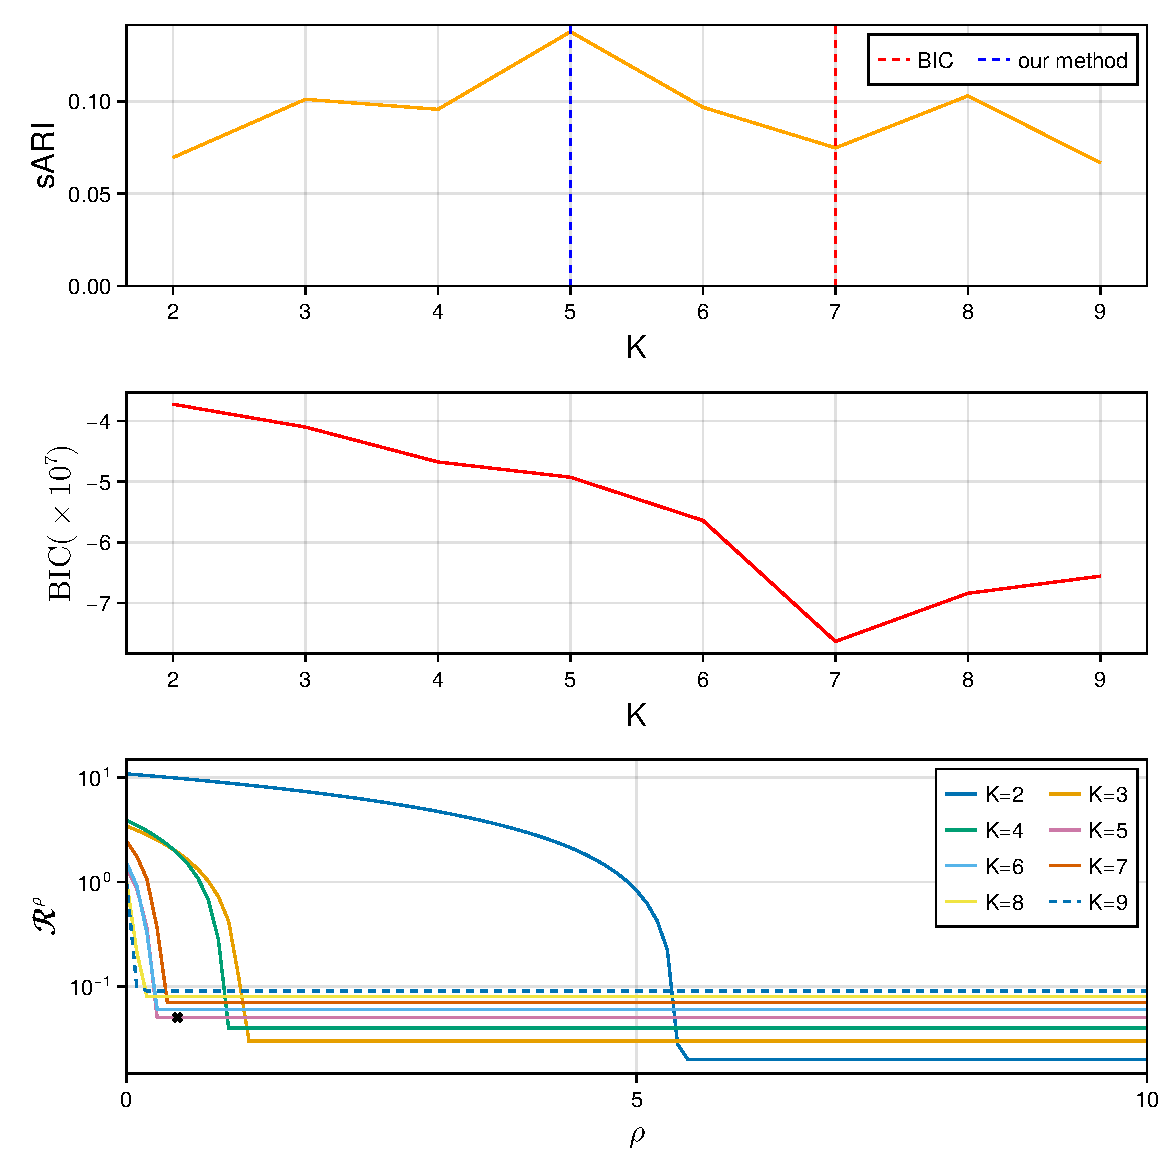
\includegraphics[width=.8\textwidth]{figures/composite-cd-urban-l2h=m1e80-shuffle-simplexh-sig=rmse-by_1e4_LInf_sparsity.pdf}
	\label{fig:urban_results_rho_k}
	\caption{
		Model selection of end-members for hyperspectral urban dataset (\cref{sec:hyperspectral}).
		\textbf{(top)} Quality of solution measured by sARI, showing $K=5$ is the solution with  material distribution that best matches the ground truth.
		\textbf{(middle top)} Quality of solution ranked using BIC, indicating $K=7$ is the best fitting solution.
        \textbf{(middle bottom)} Scree plot generated from the dataset, indicating that $K=3$ is the optimal choice of $K$.
		\textbf{(bottom)} Structurally aware loss for $K=2,\dots,9$, the wide region with the smallest $\rho$ is marked by the cross mark, indicating $K=5$ is the most appropriate choice of $K$.
	}
	\label{fig:urban_results}
\end{figure}

We obtain point estimates of the factorization using a modified implementation of the coordinate descent method \citep{Cichocki-Phan_coorddesc_2009}.
% Assuming the data follows the model in \cref{eq:Normal_PMF} with the same variance for all components, the variances can be estimated as 
% \[
% 	\widehat\sigma^{2}_{k,d} = \widehat\sigma^2_d = \frac{1}{KN(D-K+1)}\sum^{N}_{n=1}\norm{x_{nd} -\sum^{K}_{k=1}{\phi}^{(K)}_{kd}z^{(K)}_{nk}}^{2}_{2}.
% \]
We judge the quality of the estimates by quantifying how close the inferred material abundances are
%, indicated by the simplices $\lrb{z^{(K)}_{n,1},\dots,z^{(K)}_{n,K}}\transpose$, are 
to the ground truth
%In order to quantify this measure, we 
using the soft adjusted Rand index \citep[sARI;][]{Flynt_sARI_2019}.
%, a way to evaluate the similarity between two soft (probabilistic) partitions.
%Again, we compare our evaluations to BIC.
%Quantitative results are shown in .
\Cref{fig:urban_results} shows that \methodname selects $\widehat{K}=K_{o} =5$,
which also agrees with the sARI. %, also indicating that $K=5$ yields material abundance closest to ground truth.
BIC overfits, selecting $\widehat{K} = 7$, while PA underfits, selecting $\widehat{K}=3$.
\Cref{fig:hyprunmix_gt}(b)--(e) provides a qualitative understanding of the result.
%providing intuition to the performance gaps seen in \cref{fig:urban_results_rho_k}.
The small gap between $K=3$ and $K=4$ can be explained through the addition of the ``grass'' material.
However, since ``grass'' and ``tree'' are fairly similar to each other, this gap is not very large.
The large gap between $K=4$ and $K=5$ can be explained by the addition of the ``asphalt'' material -- a meaningful and significant contribution.
Finally, $K=6$ only adds a ``residual'' material compared to $K=5$, which can be interpreted as a different shade of ``grass''
and is clearly an artifact of overfitting.
%Accordingly, this is reflected in the fact that there is no gap between $K=5$ and $K=6$.

\section{Case Study: Cell Type Discovery using Single-Cell RNA Sequencing Data} \label{sec:case-study}

%To demonstrate the benefits of \methodname on a challenging problem that is , we   
Cell type discovery from single-cell RNA sequencing (scRNA-seq) data is a common task in bioinformatics workflows  
that is currently solved using complicated heuristic workflows. 
%As such, it provides a practically important  \methodname 
We first compare our default discrepancy measure choice (KL divergence) to 
the problem-specific choice of the Wasserstein distance with cosine distance, using the Sinkhorn distance as an estimator. %, ensuring a more comprehensive assessment. 
Next, we illustrate the automation of \methodname using the approach described in \cref{sec:choosing-rho}, 
which provides comparable results to those obtained through manual selection.
Finally, we highlight the superior performance of our approach compared to state-of-the-art scRNA-seq clustering pipelines.
%,  helps mitigate the common issue of cluster overestimation in existing methods.
% Additionally, we compare our default discrepancy measure -- KL divergence -- to a problem-specific choice of the Wasserstein distance with cosine distance in \cref{supp:div_comp}, using the Sinkhorn distance as an estimator.

\subsection{Setup}

We use the Tabula Muris dataset \citep{mice}, a single-cell transcriptome collection covering nearly 100,000 cells from 20 different mouse tissues with ground-truth cell types available for each observation.
% Specifically, for a given cell $j$, the observed expression profile is modeled as a draw from a mixture of Gaussians with mean $\mu_k$ and covariance $\Sigma_k$ such that $x_{\cdot j}\sim p(x) = \sum_{k=1}^{K_o} \eta_k \cdot N(x|\mu_k,\Sigma_k)$ where $\eta_k$ is the probability that an observation belongs to cluster $k$ and $\sum_{k=1}^{K_o} \eta_k = 1 $.
% \NA{To ensure a fair evaluation of clustering performance, we subsample datasets to reflect real-world scenarios with varying cell type proportions.}
To systematically evaluate performance across a range of realistic scenarios, we construct two dataset types.
In the main text we provide results for 80 \textsf{uniform} datasets which have equally sized clusters and the number of clusters varies from 2 to 16 (see \cref{tab:subsampled-datasets}).
We provide results for 15 \textsf{non-uniform} datasets in which the cluster sizes are unequal in \cref{sec:non-unif-data}.
All datasets undergo the same preprocessing steps, including filtering of low quality observations, log normalization, and dimensionality reduction via PCA.
Details of the datasets and preprocessing pipeline are provided in \cref{sec:rna-data}.

Following common practice in single-cell clustering,  we assume that the log-transformed gene expression counts $x_{nd}$
follow a Gaussian mixture model, where each cluster corresponds to a distinct cell type.
Hence, the model is clearly misspecified and so a robust clustering approach is needed.
We evaluate cell clustering performance by examining both the accuracy of cluster assignments and the precision in estimating the number of cell types.
For each dataset, we (1) check the difference in the estimated number of cell types $\widehat K$ from the true
number of cell types $K_o$ and (2) quantify the agreement between the ground truth labels and the estimated labels using the Adjusted Rand Index (ARI) and Adjusted Mutual Information (AMI) \citep{ari,ami}.

\begin{figure}[h!]
	\centering
	\subfloat{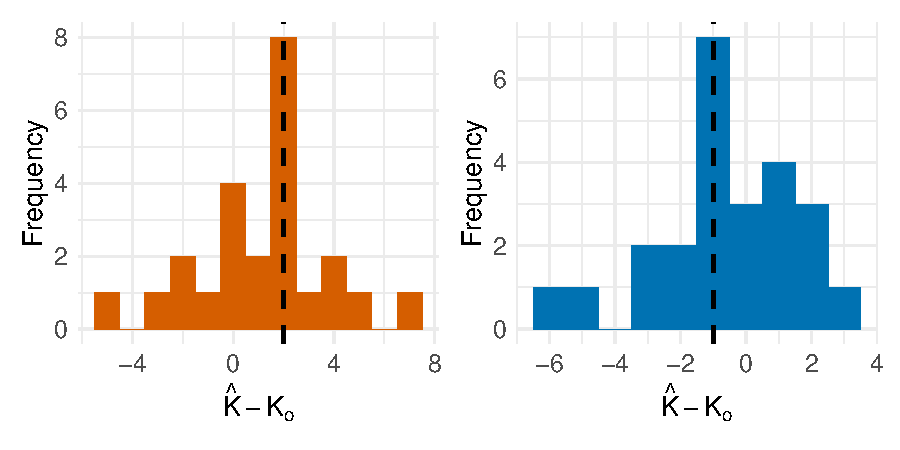
\includegraphics[width=.55\textwidth]{sh_kl_hist.pdf}}
	\subfloat{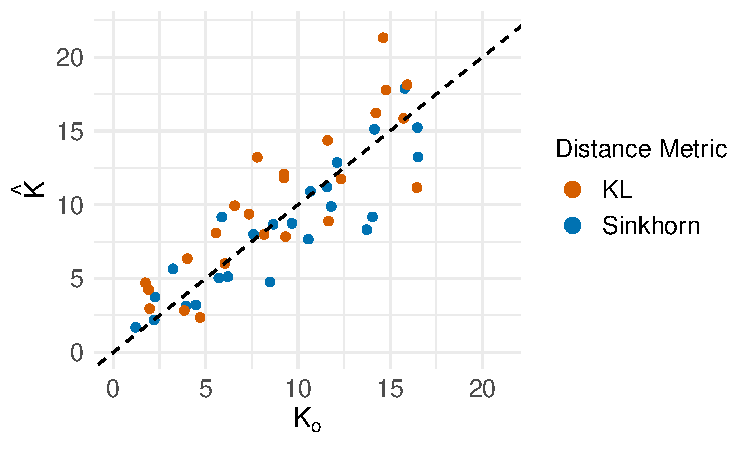
\includegraphics[width=.44\textwidth]{sh_kl_dots.pdf}}
	%\subfloat{\includegraphics[width=50mm]{figures/sh_k_diff.png}}

	\caption{Comparison of KL to Sinkhorn as divergence estimators for scRNA-seq clustering. \textbf{Left:} Difference in $K$ estimates using \methodname with KL divergence.
		\textbf{Middle:} Difference in $K$ estimates using \methodname with Wasserstein distance.
		The dashed vertical lines indicate the medians.
		\textbf{Right:} True number of cell types vs. estimated number of cell types (jittered).
	}
	\label{fig:sh_kl_comp}
\end{figure}

\subsection{Comparison of Divergences}

One benefit of \methodname is that the user can select a discrepancy measures
that best captures the underlying structure of the data.
%and hence makes the framework suitable for diverse clustering scenarios. 
While the KL divergence is our recommended default,
the Wasserstein distance can better align with the underlying metric structure of the data.
For single-cell clustering, the cosine distance is able to capture the directional relationship between gene expression profiles.
This is particularly useful with high-dimensional scRNA-seq data where the magnitude of total gene counts in each cell can vary
significantly, while the expression proportions across genes remain informative. %Sinkhorn divergence are two widely used distance metrics.
%
For numerical experiments, we use the bias-corrected KL estimator (\cref{sec:kl-estimation}) and the unbalanced Sinkhorn distance to estimate the Wasserstein distance.
See \cref{sec:case-study-details} for details.
%with parameter setting described in supplemental material.
%
% The Unbalanced Sinkhorn \citep{unbsinkhorn} solves the unbalanced Optimal Transport (OT) problem that
% \[
% 	d_{M,\varepsilon, \rho}(r, c) = \min_{P \in U(r, c)}  \langle P, M \rangle + \varepsilon \cdot \mathrm{KL}(P \| rc^T)
% 	+ \rho_1 \cdot \mathrm{KL}(P {1} \| r)
% 	+ \rho_2 \cdot \mathrm{KL}(P^T {1} \| c),
% \]
% where $P$ is the transport plan and  $r$ and $c$ are probability vectors.
% Higher weight $\varepsilon$ on estimated divergence from independence transport plan $rc^T$ (max entropy) encourages smoother transport plans which are numerically stable and less sensitive to small changes in $M$.
% Smaller marginal penalty $\rho$ introduces robustness to the marginal constraints of the transport plan.
% The balanced OT is retrieved in the limit of $\rho \to + \infty$.
%
% In our experiments, the cost matrix
% $M$ is computed based on For low-dimensional data, we impose a higher marginal penalty to recover the balanced OT problem. To account for the increased noise introduced by higher-dimensional data, we relax the marginal constraint as the data dimensionality increases.

%\NA{To evaluate the performance of our framework with the Sinkhorn distance and KL divergence, we applied both approaches to the uniform cluster data across three replications.}
%
As illustrated in \cref{fig:sh_kl_comp}, both choices of discrepancy lead to good estimates of the true number of cell types
in each dataset.
%In the scatter plot, the estimated number of cell types $\widehat{K}$ lies close to the true value $K_o$, with most trial points near the diagonal line. 
However, the KL divergence version has a bias toward overestimation (median difference of $2$ from the ground-truth $K_o$),
while the Wasserstein version has slight bias toward underestimation (median difference of $-1$).
%with a range from $-6$ to 3, 
%showing a slight bias toward underestimation. % ($\widehat{K} < K_o$), which
These results demonstrate the robustness of our default choice (KL divergence) while also highlighting the benefits of being able to improve performance by making a problem-specific choice (the Wasserstein distance).
Since we view underestimation as preferable to overestimation (i.e., overfitting),
for our remaining experiments we consider only the Wasserstein distance variant.



\subsection{Effectiveness of Automation}

To achieve accurate estimation of the number of clusters $K_o$, the application of \methodname requires careful selection of the regularization parameter $\rho$. Automating the selection of $\rho$ can reduce the need for manual intervention, particularly when applied to a large number of datasets.
Here, we apply the automated approach proposed in \cref{sec:choosing-rho}.
%based on the penalized loss graph that leverages the same intuition used for selecting $\rho$ by tracking the convergence of the penalized loss for each $K$ value.
%
%Specifically, we determine the interval of $\rho$ over which each $K$-specific loss remains optimal. The starting point of this interval is identified as the $\rho$ value where the $K$-specific loss first becomes the minimum among all losses, and the endpoint is the $\rho$ value where this loss is surpassed by the loss for a different $K$. By setting a threshold for the length of this stability interval, we can automatically select the $K$ value corresponding to the first loss function that satisfies this criterion.
%This automation approach allows users to adjust the interval threshold to balance the tradeoff between avoiding underfitting with smaller intervals and ensuring more conservative and stable $K$ selections with wider intervals.
%     #####################
%
%
%To compare the clustering performance of our method with automatically and manually selected $K$, we analyzed pairwise differences in ARI and AMI across clustering results of the uniform cluster data and evaluate their difference in estimating the number of cell types.
% their accuracy in estimating the true number of cell types $K_o$. 
As shown in Fig.~\ref{fig:auto_comp_unif},
% both methods tend to slightly underestimate the true count, likely due to some cell types being rare.
the manually selected $K$ achieves slightly better ARI values
% (ranging from $-0.04$ to $0.06$)
(ranging from $-0.27$ to $0.37$), while automated $K$ selection results in higher AMI values
% (ranging from $0$ to $0.12$). 
(ranging from $-0.19$ to $0.33$).
To assess whether the differences are significant, we conduct paired t-tests on the AMI and ARI scores. For AMI, the mean
difference between the two methods is $0.0027$  (95\% CI: $[-0.0095, 0.0148])$.
For ARI, the mean difference is $0.0084$ (95\% CI: $[-0.0069, 0.0237])$.
%In both cases, the confidence intervals included zero, indicating 
Hence, there appears to be no practically significant difference between the automated and manual approaches in terms of the two evaluation metrics.
% hence the manual and automatic methods yield comparable clustering performance.
% For both metrics, the differences are minor, with 13 out of 15 values within a magnitude of $0.02$, 
% suggesting that automated $K$ selection achieves clustering agreement comparable to that of manual selection.
%Overall, both methods demonstrate similar clustering performance across ARI, AMI, and cell type estimation.


\begin{figure}[t!]
	\centering
	\subfloat{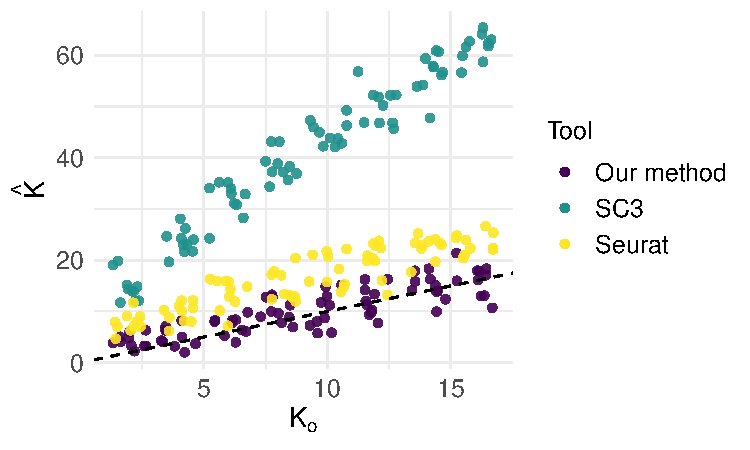
\includegraphics[height=.34\textwidth,trim=0in 0in 1.35in 0in,clip]{tool_comp_estk.pdf}}
	\subfloat{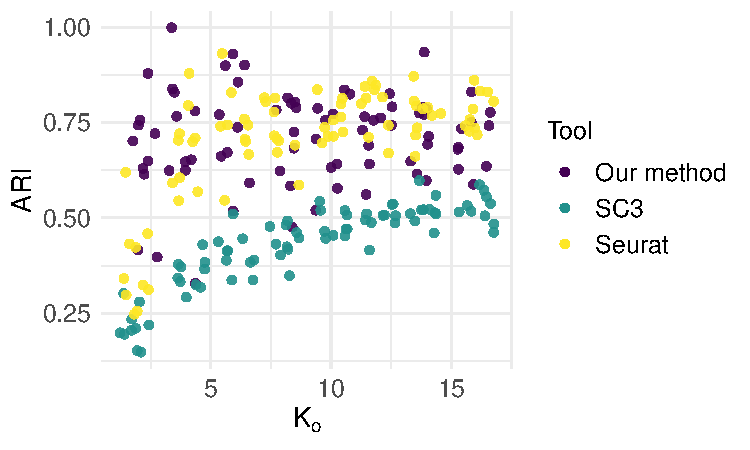
\includegraphics[height=.34\textwidth]{tool_comp_ari.pdf}}
	%\subfloat{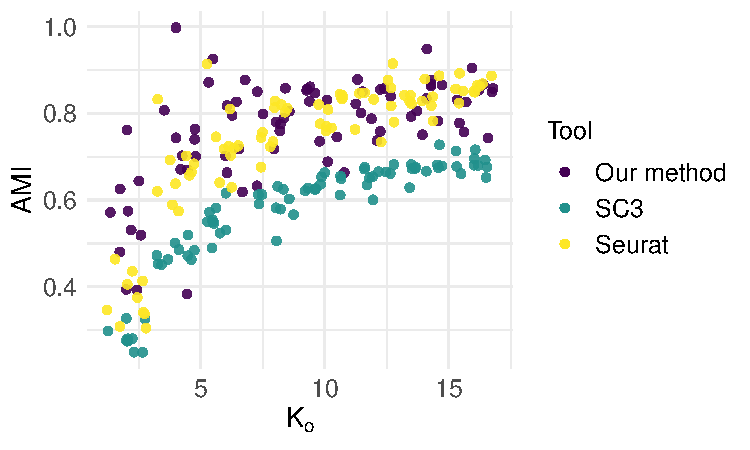
\includegraphics[height=.34\textwidth]{tool_comp_ami.pdf}}
	\caption{Comparison between \methodname and existing tools across datasets with equally
		sized clusters.
		\textbf{Left:} True number of cell types vs.\ estimated number of cell types.
		\textbf{Right:}  True number of cell types vs.\ ARI.
		%	\textbf{Right:} AMI vs. number of true cell types.
	}
	\label{fig:tool_comp_unif}
\end{figure}

\subsection{Comparison with Existing Tools}

There are many specialized tools for single-cell RNA sequencing clustering.
However, a common challenge with these tools is the tendency to overestimate the number of cell types, particularly in datasets with complex structures. In this section, we demonstrate that \methodname not only mitigates the issue of overestimation but also achieves strong clustering agreement. We compare \methodname with the popular Seurat  \citep{seurat} and SC3  \citep[Single-Cell Consensus Clustering;][]{sc3} packages; see \cref{sec:existing-tools} for further details about each tool.

% To compare the performance of our  with Seurat and SC3, we evaluated their accuracy in cell type estimation and cluster label agreements across the uniform cluster datasets with different numbers of cell types and equal cluster sizes.
\Cref{fig:tool_comp_unif} shows that \methodname has superior accuracy in cell type number estimation compared to Seurat and SC3. The estimates produced by \methodname closely track $K_o$ while Seurat and SC3 tend to overestimate $K_o$.
While Seurat shows a consistent level of overestimation for datasets with differing numbers of clusters,
SC3 overestimates the number of clusters more as $K_o$ increases.
%indicating declining performance in more challenging datasets. 
%Overall, our approach outperforms Seurat and SC3 in accurately predicting the true number of cell types.
%
In terms of clustering agreement, our framework and Seurat achieve comparable ARI and AMI values across datasets.
While ARI for Seurat and SC3 is lower in datasets with $K_{o} < 5$,
% datasets with more cell types, 
\methodname maintains stable clustering agreement across all values of $K_o$.
SC3 performs poorly on both ARI and AMI due to its significant overestimation of cell types.
Across all the \textsf{uniform} datasets, \methodname has an average ARI (respectively AMI) value of $0.71$ ($0.76$), versus Seurat's average of 0.71 (0.73) and SC3's average of 0.43 (0.57).
It is notable that our simple, general approach outperforms
two carefully engineered pipelines designed specially for clustering single-cell genomic data.


\section{Discussion} \label{sec:discussion}

While we have demonstrated the practical utility and broad applicability of \methodname to robustly discovering latent processes with real-world interpretations, that are a number of important limitations that motivate directions for future work.

First, in applications where related labeled datasets are not available, we are only able to provide a heuristic method for calibrating the degree of misspecification, as quantified by $\rho$.
Ideally, we would like to have a more rigorous criteria.
However, given the nonparametric nature of misspecification, we suspect that a fully general solution does not exist; indeed, the coarsened posterior similarly requires a heuristic calibration step.
One alternative to explore in future is the simulation-based calibration method from \citet{Xue:2024}, which was developed for the coarsened posterior but could easily be used with \methodname as well.
However, generally speaking, a user must have \emph{some} prior knowledge about the degree of model misspecification -- and believe that the misspecification will be reasonably small as measured by the chosen discrepancy.
Moreover, if the degree of misspecification is very large, we should not expect any robust model selection procedure to
work well (cf.\ $P_{o}^{E}$ in \cref{fig:consistency-illustration}).

Second, our current robust consistency guarantees are limited to mixture models and matrix factorization.
It would be valuable to have a more general consistency theory that either covers other common model classes
or the general modeling framework from \cref{sec:framework}.
It would also be valuable to characterize how quickly $\Pr(\widehat{K} = K_o)$ converges to 1 and to quantify the variability of $\widehat{K}$.
Another interesting direction for future work is to apply \methodname to other model classes such as supervised factor analysis and extend it to apply to more flexible models such as (nonlinear) variational autoencoders \citep{Kingma2014,Kingma2019VAEs} and semiparametric matrix factorization models \citep{Anandkumar2014uc,rohe2023vintage-7f4}.

Finally, \methodname does not provide any uncertainty quantification.
A Bayesian version of our method that provides a distribution over $K$ would be useful,
as it could quantify uncertainty in $K$ even as $N \to \infty$.
A fully generalized Bayesian version that simultaneously quantifies parameter uncertainty would also be valuable.
\section*{Acknowledgments}


\bibliographystyle{imsart-nameyear}
\bibliography{paper-ref}

\newpage
\appendix
% !TEX root =  manuscript_arxiv.tex

\counterwithin{equation}{section}
\counterwithin{figure}{section}
\renewcommand{\thefigure}{\Alph{section}.\arabic{figure}}
\counterwithin{table}{section}
\renewcommand{\thetable}{\Alph{section}.\arabic{table}}
\counterwithin{theorem}{section}
\renewcommand{\thetheorem}{\Alph{section}.\arabic{theorem}}
\counterwithin{lemma}{section}
\renewcommand{\thelemma}{\Alph{section}.\arabic{lemma}}


\begin{center}
    \LARGE \textbf{Supplementary Materials}
\end{center}

%\begin{lemma}
%	Suppose $\mathcal{I}$ and $\mathcal{I}'$ are two disjoint sets for $\{1,\ldots, K\}$. For two sets of coefficients $a_k, b_{k'}$, suppose $a_k\neq0$ for $k \in \mathcal{I}$, $a_k=0$ for $k \in \mathcal{I}'$,  $b_{k'}=0$ for $k' \in \mathcal{I}$ and $\sum_{k\in \mathcal{I}} a_k = 1$ and $\sum_{k'\in \mathcal{I}'}b_{k'} = 1$. Then there exist coefficients $\gamma_{kk'}$ such that $\sum_{k\in\mathcal{I}, k'\in\mathcal{I}'}\gamma_{kk'}=1$.
%	
%\end{lemma}


\section{[out-of-date] Robust Model Selection Consistency} % of Structurally Aware Robust Model Selection
\label{sec:theory}

\PROBLEM{TODO: integrate material from this section into the appendix}

We now show that, under reasonable assumptions, our model selection procedure is robustly consistent.
Then, in light of our results, we discuss some specific choices of discrepancy measure.
Here we emphasize the assumptions required in the mixture modeling case, since the probabilistic matrix factorization assumptions are similar but require more notation to state;
see \cref{sec:PMF-consistency-proof} for details.

\subsection{Assumptions}


%We now show that our model selection procedure consistently estimates $K_{o}$ under reasonable assumptions.

%Let $\mcX$ and $\paramspace$ be spaces for observations and parameters, respectively. Assume family of distributions $\mathcal{F} = \{f_{\param}: \param \in \paramspace\}$ where $f_{\param}$ are absolutely continuous with respect to some base measure $\lambda$ on $\paramspace$.
%Denote the true number of components as $\numcomps_o$ and $F_{ok}$ as the true underlying distribution for component $k = 1, \ldots, \numcomps_o$. 
%We show that  structurally aware model selection rule achieves the consistency of number of components.
%Our assumptions are mild. 
First, we consider the requirements for the discrepancy $\discr{\cdot}{\cdot}$ and, when applicable, the discrepancy estimator $\discrest{\cdot}{\cdot}$
-- noting that sometimes it will be possible to take $\discrest{\cdot}{\cdot} = \discr{\cdot}{\cdot}$.
%We require the smoothness and the existence of a consistent estimator for discrepancies $\discr{P}{Q}$.
For some discrepancies such as the Kullback--Leibler divergence, $\discr{P}{Q} < \infty$ only if $P$ is absolutely continuous with respect to $Q$.
However, since we require an empirical estimate of each component distribution, absolute continuity may not hold.
Therefore, we introduce a possibly weaker metric $d$ on probability measures that detects convergence of empirical measures.
%satisfies $d(P, Q_{N}) \to 0$ as $N \to \infty$
%whenever $Q_{N} \to P$ in distribution. %   such which converges to zero whenever $Q$ converges to $P$ in distribution and can be bounded by a function of $\discr{P}{Q}$. 
%We also require some other modest regularity conditions on $d$ and $\mcD$, presented in \cref{assump:metric-discr-conditions}.
\begin{assumption} 	\label{assump:metric-discr-conditions}
	%Let $y_{1}, y_{2}, \dots$ be independent samples from distribution $P$, and denote 
	For $y_{\numobs n} \in \mathcal{X}$ $(\numobs = 1,2,\dots; n = 1,\dots,\numobs)$,
	define the empirical distribution $\widehat{P}_{\numobs} = \numobs^{-1}\sum_{n=1}^{\numobs}\delta_{y_{N,n}}$
	and assume $\widehat{P}_{\numobs} \rightarrow P$ in distribution.
	The metric $d$, discrepancy $\mcD$, and estimator $\widehat{\mcD}$ satisfy the following conditions:
	%\begin{enumerate}[(a)]
	\begin{enumerate}[label=\textnormal{(\alph*)}]
		\item \emph{The metric detects empirical convergence:} $d(\widehat{P}_\numobs, P) \to 0$ as $\numobs \to \infty$.
		\item  \emph{The metric is jointly convex in its arguments:} for all $w \in (0, 1)$ and distributions $P$, $P'$, $Q$, $Q'$,
		      \[
			      d(wP + (1 - w)P', wQ + (1 - w)Q') \le w\,d(P, Q) + (1 - w)\,d(P', Q').
		      \]
		      %$d(\sum_{i=1}^{n}w_i P_i, \sum_{i=1}^{n}w_i Q_i) \leq \sum_{i=1}^{n} w_i d(P_i, Q_i)$ for $0\leq w_i \leq 1$ and $\sum_{i = 1}^n w_i = 1$;
		      %	\item  \emph{The metric is bounded:} there exists a constant $M < \infty$ such that
		      %	$d(P,Q) \le M$ for all distributions $P, Q$. 
		\item  \emph{The discrepancy estimator is consistent:} For any distributions $P, Q$,
		      if $\discr{P}{Q} < \infty$ and $\widehat P_{N} \to P$ in distribution,
		      then $\discrest{\widehat{P}_{\numobs}}{Q} \to \discr{P}{Q}$ as $\numobs \to \infty$.
		\item \emph{Smoothness of the discrepancy estimator:} The map $\param \mapsto \discrest{\widehat{P}_{\numobs}}{F_{\param}}$ is continuous.
		\item  \emph{The discrepancy bounds the metric:} There exists a continuous,
		      non-decreasing function $\kappa: \reals \to \reals$ such that
		      $d(P,Q) \leq \kappa(\discr{P}{Q})$ for all distributions $P, Q$.
		\item \emph{The metric between components is finite:} For all $\param, \param' \in \Theta$,
		      we have $d(F_{\param}, F_{\param'}) < \infty$.
	\end{enumerate}
\end{assumption}

A wide variety of metrics satisfy \cref{assump:metric-discr-conditions}(a), including the bounded Lipschitz metric,
the Kolmogorov metric, maximum mean discrepancies with sufficiently regular bounded kernels, and the Wasserstein metric with a bounded cost function \citep{Vaart:1996,Sriperumbudur:2010,SimonGabriel:2018,Villani:2009}.
%requires metric $d$ to characterize the convergence of empirical process. For example, all metrics fall into the Glivenko--Cantelli class are able to provide the uniform convergence of empirical average to the true distribution in probability. This generally holds for a range of metrics including bounded Lipschitz and Kolmogorov metrics by \citep{Vaart:1996}.
%\cref{assump:metric-discr-conditions}(b) and \cref{assump:metric-discr-conditions}(c) admit the joint convexity and the boundedness of the metric, respectively. 
%The joint convexity property
\Cref{assump:metric-discr-conditions}(b) also holds for a range of metrics.
%For example, define integral probability metrics as 
%$\gamma_{\mathcal{H}}(P,Q) = \sup\{\vert \int_S f dP - \int_S f dQ \vert: f \in \mathcal{H} \}$, where $P$ and $Q$ are probability measures defined on space $S$ and $\mathcal{H}$ is a class of real-valued bounded measurable functions on $S$. 
For example, it is easy to show that all integral probability metrics -- which includes the bounded Lipschitz
metric, maximum mean discrepancy, and 1-Wasserstein distance -- are jointly convex (see \cref{lem:ipm-joint-convex} in the Appendix).
\cref{assump:metric-discr-conditions}(c) is a natural requirement that the limiting divergence can be estimated consistently.
Such estimators are well-studied for many common discrepancies.
%We discuss consistent estimation of the Kullback--Leibler divergence in \cref{sec:kl-estimation}.
\cref{assump:metric-discr-conditions}(d) will typically hold as long as the map $\phi \mapsto F_{\phi}$ is
well-behaved.
For example, for the Kullback--Leibler divergence estimators described in \cref{sec:kl-estimation}
and standard maximum mean discrepancy estimators \citep{Gretton:2012,Krause:2023},
when $F_{\phi}$ admits a density $f_{\phi}$, it suffices for the map $\phi \mapsto f_{\phi}(x)$
to be continuous for $P_{o}$-almost every $x$.
\cref{assump:metric-discr-conditions}(e) is not overly restrictive and we discuss some relevant examples in \cref{sec:divergence-choice} below.
%. See \citet{Gibbs:2002} for a extensive overview
%of the relationships between common metrics and divergences.
\cref{assump:metric-discr-conditions}(f) trivially holds for bounded metrics such as the bounded Lipschitz metric and integral probability measures with uniformly bounded test functions.

Our second assumption requires the parameter estimation procedure to be sufficiently well-behaved,
in the sense that, for each fixed number of components $\numcomps$, it should consistently estimate an asymptotic parameter $\allparam_{\star}^{(K)}$.
We do not make any explicit assumptions that such parameters are, in any sense, ``optimal.''
% quantifies the regularity of the inference algorithm and provides guarantees on contracting the convergence of empirical distribution to its limiting distribution.

\begin{assumption}\label{assump:inference-regularity}
	For each $\numcomps \in \{1,\dots, \numcomps_{o}\}$, there exists $\theta_{\star}^{(K)} \in \paramSpace{K}$ such that
	$\widehat\theta^{(K)} \to \theta_{\star}^{(K)}$ in probability as $N \rightarrow \infty$,
	after possibly reordering of components.
\end{assumption}
To simplify notation, we will write $F^{(K)}_{\star k} = F_{\param^{(K)}_{\star k}}$ and $G^{(K)}_{\star k} = G_{\allparam^{(K)}_{\star k}}$, and similarly for their densities.
\Cref{assump:inference-regularity} holds for most reasonable algorithms, including expectation--maximization, point estimates based on the posterior distribution,
and variational inference \citep{Balakrishnan:2017,Walker:2001,Wang:2019}.
Note that we assume that consistency holds for parameters in the equivalence class induced by component reordering, although we keep
this equivalence implicit.
\Cref{assump:inference-regularity} implies that the empirical data distribution of the $k$th component,
$\widehat{F}^{(K)}_k$, % = |X_{k}(z^{(K)})|^{-1}\sum_{x \in X_{k}(z^{(K)})} \delta_{x}$,
converges to a limiting distribution
% $\widetilde{P}^{(K)}_k$ that depends on $P_{o}$ and the limiting 
%parameters $\allparam_{\star}^{(K)}$:
%For fixed $\numcomps$ and each $k \in \{1,\dots,\numcomps\}$, denote the empirical weights and component distributions 
%by, respectively, $\eta^{(K)}_{\star k} = |X_{k}(z^{(K)}_{1:N})|/\numobs$
%and . 
%Define $\widetilde{F}^{(K)}_k$ as the limiting distribution of $\widehat{F}^{(K)}_k$ as
\begin{align}
	\widetilde{F}^{(K)}_{k}(\dee x) & = \frac{p_{\star}^{(K)}(k\mid x)P_o(\dee x) }{\int p_{\star}^{(K)}(k\mid y)P_o(\dee y)}, \label{eq:phat-def}
\end{align}
where $p_{\star}^{(K)}(k \mid x) = \eta^{(K)}_{\star k}f_{\star k}^{(K)}(x)/p^{(K)}_{\star}(x)$ is the
conditional component probability under the limiting model distribution.
%The limiting distribution $\widetilde{P}^{(K)}_k$ depends on the optimal parameter from the inference algorithm. 

%Denote the model optimal weights and distributions as $\eta_k^\star$ and $F^{\star}_{k}  (k=1, \ldots, \numcomps)$. 

Our third assumption concerns the regularity of the data distribution and model.
\begin{assumption} \label{assump:model-conditions}
	The data-generating distribution $P_o$ and component model family $\mcF$ satisfy the following conditions:
	%\begin{enumerate}[(a)]
	\begin{enumerate}[label=\textnormal{(\alph*)}]
		\item \emph{Meaningful decomposition of the data-generating distribution:} for positive integer $\numcomps_{o}$, $\eta_{o} \in \Int{\Delta_{\numcomps_o}}$ (the interior of $\Delta_{\numcomps_o}$), and distributions $F_{o1},\dots,F_{o\numcomps_{o}}$ on $\mcX$, it holds that $P_{o} = \sum_{k = 1}^{K_o}\eta_{ok}F_{ok}$.
		\item \emph{Accuracy of the parameter estimates for $\numcomps = \numcomps_{o}$:} There exists $\rho > 0$
		      such that for each $k \in \{1, \ldots, \numcomps_o\}$, it holds that
		      $\discr{\widetilde{F}_{k}^{(K_{o})}}{F^{(K_{o})}_{\star k}} < \rho$.
		\item \emph{Poor model fit when $\numcomps$ is too small:} For the same $\rho$ as part (b),
		      for any $\numcomps < \numcomps_o$, it holds that $d(P_o, P_{\star}^{(\numcomps)}) > \kappa(\rho) $.
	\end{enumerate}
\end{assumption}

\cref{assump:model-conditions}(a) formalizes the decomposition of the data-generating distribution into real-world processes that we aim to recover.
% the true number of latent sub-populations by parametrized finite mixture models given the presence of model misspecification.
\cref{assump:model-conditions}(b) requires that, when the number of components is correctly specified,
the divergence between the asymptotic empirical component distribution $\widetilde{F}^{(\numcomps_{o})}_{k}$ and the asymptotic component
$F_{\star k}^{(\numcomps_{o})}$ is small for each component $k \in \{1,\ldots,\numcomps_{o}\}$.
In \cref{subsec:theory-rho-bounds}, we give conditions under which $\discr{F_{ok}}{F^{(K_{o})}_{\star k}} < \rho_{o}$
implies the assumption holds for the Kullback--Leibler divergence and integral probability metrics with bounded test functions. % in \cref{prop:kl-upper-bound,prop:IPM-metric-upper-bound}.

\cref{assump:model-conditions}(c) formalizes the intuition that model selection will only be successful if, when the number of components is smaller than the true generating process,
the mixture model is a poor fit to the data.
For example, if $K_o = 2$, $F_{o1} = \distNorm_-(0, \sigma^2)$ and $F_{o2} = \distNorm_+(0, \sigma^2)$ (the normal distribution truncated to either negative or positive values), and $\eta_{o1} = \eta_{o2} = 0.5$, then clearly a one-component Gaussian mixture can fit the model perfectly since $P_o = \distNorm(0, \sigma^2)$.
Hence, any reasonable model selection procedure would asymptotically select $\widehat K = 1$.
\cref{assump:model-conditions}(c) forbids such pathological setups.
The necessary degree of mismatch depends on the match between the true and estimated component distributions (which depends on the choice of $\mcD$ and is measured by $\rho$)
and the relationship between $\mcD$ and $d$ (which is described by $\phi$).
% and the mismatch between the 
%true component probabilities (as measured by $\bar{\eta} = \sum_{k=1}^{\numcomps_{o}} |\eta_{ok} - \eta_{\star k}| = \|\eta_{o} - \eta_{\star}\|_{1}$). 
%Even with well-specified model assumptions, the distance between the mixture model and the true density given the optimal parameters $\param^{\star}$ should be large.

\subsection{Main Results}

\PROBLEM{TODO: move versions of these to previous section}
%The following result provides a general framework to establish when our method consistently estimates $K_{o}$ in the mixture model setting. %for estimating the number of components.
%Our proof breaks into two parts: first we show that when $\numcomps = \numcomps^\star$, the modified log-likelihood attains the maximum in probability; second, we show for any $\numcomps < \numcomps^\star$, the modified log-likelihood will be large indicating that the model is inadequate. 
%\NA{For simplicity, we use a shorthand notation to denote $\mcR^{\rho}_{\numobs} (\param^{(\numcomps)};\data{})=\mcR^{\rho}(\param^{(\numcomps)};\data{1:\numobs})$ and $\mcR^{\rho,\lambda}_{\numobs}(\param^{(\numcomps)};\data{}) =\mcR^{\rho,\lambda}(\param^{(\numcomps)};\data{1:\numobs})$.}\fTBD{I don't think this really makes the notation any cleaner. Maybe use it in the proof if you can remove explicit dependence on $x$. But not worth using to state the theorem.}
To state our main results, let $\widehat{\numcomps}_{\numobs}(\rho)$ denote the
output of \cref{algo:model-selection-general} given $\data{1:\numobs}$ and the specified value of $\rho$.
%$ = \widehat{\numcomps} = \argmin_{\numcomps} \mathcal{R}^{\rho,\lambda}(\widehat\allparam^{(\numcomps)}; z^{(\numcomps)}, \data{1:\numobs})$ denote the structurally aware robust model choice.

% the number of components selected by structurally aware robust inference.
\begin{theorem} \label{thm:main}
	For mixture modeling, if \crefrange{assump:metric-discr-conditions}{assump:model-conditions} hold, then $\Pr\{\widehat{\numcomps}_{\numobs}(\rho) = K_{o}\} \to 1$ for $N \to \infty$.
	%the consistency of number of components holds for structurally aware model selection, i.e., 
	%Then for $\rho > \rho^{\star}$
	%	\begin{enumerate}[(1)]
	%		\item for $\numcomps = \numcomps_o$,  $ \mcR^{\rho}_{\numobs}(\param_{\star}^{(\numcomps)};\data{}) \rightarrow 0$ in probability as $\numobs \rightarrow \infty$. 
	%		\label{thm:maxloglik-with-trueK}
	%		\item for $\numcomps < \numcomps_o$, $\mcR^{\rho}_{\numobs}(\param_{\star}^{(\numcomps)};\data{})\rightarrow \infty$ in probability as $\numobs \rightarrow \infty$.
	%	\end{enumerate}
	%$$\widehat{\numcomps}_{\numobs}(\rho) \rightarrow \numcomps_{o} \ \text{in probability as} \ \numobs \to \infty.$$
\end{theorem}
\begin{proof}[Proof idea] To prove \cref{thm:main} we establish two facts.
	First, we show that the loss satisfies
	\[
		\Pr\{\mcR^{\rho}(\allparam^{(\numcomps_{o})}; z^{(\numcomps_{o})}, \data{1:\numobs}) = 0 \}   \overset{N \to \infty}{\longrightarrow}  1.
	\]
	Second, we verify that for $\numcomps < \numcomps_o$,
	$
		\mcR^{\rho}(\allparam^{(\numcomps)}; z^{(\numcomps)}, \data{1:\numobs}) \to \infty
	$
	in probability for $N \to \infty$.
	Therefore, for $\numcomps > \numcomps_o$, asymptotically
	$\mcR^{\rho}(\allparam^{(\numcomps)}; z^{(\numcomps)}, \data{1:\numobs})  \ge \mcR^{\rho}(\allparam^{(\numcomps_{o})}; z^{(\numcomps_{o})}, \data{1:\numobs})$, so the minimum is asymptotically attained at $\widehat{\numcomps}=\numcomps_o$.
\end{proof}

Under generally analogous conditions, a similar result holds for probabilistic matrix factorization.
We defer the statements and discussion of the assumptions to \cref{sec:PMF-consistency-proof}. %, which also includes the proof of \cref{thm:main-pmf}.
Also, due to the greater complexity of the dependence structure, we restrict our attention to case where the discrepancy is the KL divergence (which we use in our PMF experiments):
\begin{theorem} \label{thm:main-pmf}
	For probabilistic matrix factorization, if \cref{assump:metric-discr-conditions,assump:consistency,assump:sample_approx_able,assump:data_regular} hold, then $\Pr\{\widehat{\numcomps}_{\numobs}(\rho) = K_{o}\} \to 1$ as $N \to \infty$.
\end{theorem}
%Due to the similarity of the assumptions to those in the mixture modeling case,

While \cref{thm:main,thm:main-pmf} guarantee robust consistency under quite general and intuitive conditions, these results leave two important questions open to make the theory satisfactory.
First, what choices of $\mcD$ and $d$ can satisfy \cref{assump:metric-discr-conditions} (and for what choice of $\kappa$)?
Second, while \cref{assump:model-conditions} requires that $\discr{\widetilde{F}_{k}^{(K_{o})}}{F^{(K_{o})}_{\star k}} < \rho$
(and something similar is required by \cref{assump:data_regular} in the PMF case),
it is more natural to require a bound on $\discr{F_{ok}}{F^{(K_{o})}_{\star k}}$.
Does a bound on the latter imply the former?
We address these questions next in \cref{sec:divergence-choice,subsec:theory-rho-bounds}.
%makes it clear that, when applying our method in practical scenarios, the choice of divergence $\mcD$ and the selection of the cutoff value $\rho$ are crucial.
%For choice of divergence $\mcD$, we require $\mcD$ satisfy our assumptions in \cref{assump:metric-discr-conditions}.
%The following results 
%For the value of $\rho$, as indicated in \cref{assump:model-conditions}, it is contingent upon both the chosen divergence measure and the degree of discrepancy between the model component and the actual generating component distribution.
%Let's now further provide theoretical guarantees about these two crucial pieces in our methodology: the choice of divergence and the value of $\rho$.


%\begin{proof}[(assuming metric)]
%	%Consider 
%	%\begin{equation}
%	%	\widehat{P}_k(dx) = \frac{\Pr(z=k\mid x) P_o(dx)}{\int \Pr(z=k\mid y) P_o(dy) },
%	%\end{equation}
%	%where $\Pr(z=k \mid x) = \eta_{\star k}f_{\phi_{\star k}}(x)/ \sum_{\ell =1}^{K}\eta_{\star\ell}f_{\phi_{\star\ell}}(x)$ and $P_o(dx) = \sum_{\ell =1}^{K}\eta_{o\ell}P_{o\ell}(dx)$. It follows by triangle inequality that 
%	%\begin{align}
%	%d(\widehat{P}_{k}, {F_{\param^\star_{k}}})& \le d(F_{ok}, F_{\param^\star_{k}}) + d(F_{ok},\widehat P_{k}) \\
%	%& \le \rho +d\left(F_{ok},\frac{\eta_{\star k}f_{\phi_{\star k}}}{\int \eta_{\star k}f_{\phi_{\star k}}(y)  \frac{\sum_{\ell =1}^{K}\eta_{o\ell}P_{o\ell}}{\sum_{\ell =1}^{K}\eta_{\star\ell}F_{\phi_{\star\ell}}}(dy)} \frac{\sum_{\ell =1}^{K}\eta_{o\ell}P_{o\ell}}{\sum_{\ell =1}^{K}\eta_{\star\ell}F_{\phi_{\star\ell}}}\right)\\
%	%& \le \rho +d\left(F_{ok},\frac{f_{\phi_{\star k}}}{Z_k} \frac{\sum_{\ell =1}^{K}\eta_{o\ell}P_{o\ell}}{\sum_{\ell =1}^{K}\eta_{\star\ell}F_{\phi_{\star\ell}}}\right),
%	%\end{align}
%	%where $Z_k = \frac{f_{\phi_{\star k}}(y)}{\int f_{\phi_{\star k}}  \frac{\sum_{\ell =1}^{K}\eta_{o\ell}P_{o\ell}}{\sum_{\ell =1}^{K}\eta_{\star\ell}F_{\phi_{\star\ell}}}(dy)}$.
%	Consider 
%	\begin{align}
%		&\Pr(z=k \mid x) \\
%		&= \frac{\eta_{\star k}f_{\phi_{\star k}}(x)}{\sum_{\ell =1}^{K}\eta_{\star\ell}f_{\phi_{\star\ell}}(x)} \\
%		&= \frac{\left(\eta_{\star k}-\eta_{ok}\right)f_{\phi_{\star k}}(x) + \eta_{ok}\left(f_{\phi_{\star k}} - p_{ok}(x)\right)+\eta_{ok}p_{ok}(x)}{\sum_{\ell=1}^{K} \left(\eta_{\star\ell}-\eta_{o\ell}\right)f_{\phi_{\star\ell}}(x) +\sum_{\ell=1}^{K} \eta_{o\ell}\left(f_{\phi_{\star\ell}} - p_{o\ell}(x)\right)+\sum_{\ell=1}^{K}\eta_{o\ell}p_{o\ell}(x)} 
%	\end{align}
%	It follows by triangle inequality that
%	\begin{align}
%		d(\widehat{P}_{k}, {F_{\param^\star_{k}}})& \le d(F_{ok}, F_{\param^\star_{k}}) + d(F_{ok},\widehat P_{k}) \\
%		& \le \rho + d(F_{ok},\widehat P_{k})\\
%		& \le \rho + d\left(F_{ok}, \frac{\Pr(z=k \mid x)P_o(dx)}{\int \Pr(z=k \mid y)P_o(dy)}\right)
%	\end{align}
%	
%\end{proof}

\subsection{Choice of Divergence} \label{sec:divergence-choice}


While there many possible choices for the divergence, we focus on some that are statistically natural (KL divergence), computationally convenient (maximum mean discrepancy \citep[MMD; ][]{Sriperumbudur:2010}), or interpretable (1-Wasserstein distance \citep{Villani:2009}).
Specifically, we show that all three satisfy \cref{assump:metric-discr-conditions}(a,b,e) when an appropriate choice of $d$ is made.
%Finding a proper $d$ that satisfies \cref{assump:metric-discr-conditions} with a given $\mcD$ is crucial to guarantee the consistency results in \cref{thm:main}.
%We will make heavy use of integral probability metrics.
Before stating these results, we recall the following useful class of metrics on probability measures.
\begin{definition}[Integral probability metric]
	Given a collection $\mcH$ of real-valued functions on $\mcX$,
	for any probability measures $P$ and $Q$ on $\mcX$,
	the corresponding \emph{integral probability metric} is defined as
	\[ \label{eq:IPM}
		d_{\mcH}(P,Q) = \sup_{h \in \mcH}\left|\int h(x)P(\dee x) - \int h(y) Q(\dee y)\right|.
	\]
\end{definition}
\paragraph{Kullback--Leibler divergence.}
%Integral probability metrics include a broad class of metrics.
%  restricting the function class to all real-valued bounded Lipschitz functions.
Assume that $\mcX$ is equipped with a metric $m$ and define the \emph{bounded Lipschitz norm}
$\BLnorm{h} = \Vert h \Vert_{\infty} + \Vert h \Vert_{L}$, where $\Vert{h}\Vert_{L} = \sup_{x \ne y}|h(x) - h(y)|/m(x, y)$
and $\Vert{h}\Vert_{\infty} = \sup_{x} |h(x)|$.
Letting $\mcH = \mcH_{\mathrm{BL}} = \{h : \Vert h \Vert_{\mathrm{BL}}\le 1\}$ gives the bounded Lipschitz metric
$\blmetric = d_{\mcH_{\mathrm{BL}}}$.
%With  bounded Lipschitz metric, we can show that Kullback--Leibler divergence is valid to use in our algorithm.
%We can use \cref{thm:main} to prove the consistency of our method when using bounded Lipschitz metric and the Kullback--Leibler divergence.
If $\mcD$ is the KL divergence, we can choose $d$ to be the bounded Lipschitz metric.
\begin{proposition} 	\label{coro:KL}
	If $d(P, Q) = \blmetric(P,Q)$ and $\mcD(P \mid Q) = \kl{P}{Q}$, then
	\cref{assump:metric-discr-conditions}(a,b,e) holds with $\kappa(\rho) = (\rho/2)^{1/2}$.
	%Hence, if \cref{assump:model-conditions} holds, then 
	%$\widehat{\numcomps}_{\numobs}(\rho) \rightarrow \numcomps_{o}$ in probability as $N \to \infty$.
\end{proposition}

\paragraph{Maximum mean discrepancy (MMD).}
Let $\mcK $ denote a kernel.
Denote the reproducing kernel Hilbert space with positive definite kernel $\mcK \colon \mcX \times \mcX \to \reals$ as $\mcH_{\mcK}$.
Denote the inner product of $\mcH_{\mcK}$ by $\langle{\cdot},{\cdot}\rangle_{\mcK}$ and the norm by $\|{\cdot}\|_{\mcK}$.
Letting $\mcH = \mcB_{\mcK} = \{ h \in \mcH_{\mcK} :  \|h\|_{\mcK} \le 1\}$, the unit ball, gives the maximum mean discrepancy $d_{\mathrm{MMD}} = d_{\mcB_{\mcK}}$.
If we choose the divergence to be an MMD, $d$ can be the same MMD.
%Here we assume a well-defined $d_{\mathrm{MMD}}(P,Q)$ is given and we show by choosing it as both the divergence and metric the consistency of number of clusters still holds.
\begin{proposition} 	\label{coro:MMD}
	If $\mcK$ is chosen such that $d_{\mathrm{MMD}}$ metrizes weak convergence, and
	%	Assume that $d_{\mathrm{MMD}}(P,Q) = 0 \iff P = Q$ for any Borel probability measures $P, Q$ on $\mcX$ and 
	%	$d_{\mathrm{MMD}}(\widehat{P}_{\numobs}, P) \rightarrow 0$ in probability for any 
	%	$\widehat{P}_{\numobs} \rightarrow P$ in distribution.
	$d(P, Q) =  \discr{P}{Q} = d_{\mathrm{MMD}}(P,Q)$,
	then \cref{assump:metric-discr-conditions}(a,b,e) holds with $\kappa(\rho) = \rho$.
	%	Hence, if \cref{assump:model-conditions} holds, then 
	%	$\widehat{\numcomps}_{\numobs}(\rho) \rightarrow \numcomps_{o}$ in probability as $\numcomps \to \infty$.
\end{proposition}

For conditions under which $d_{\mathrm{MMD}}$ metrizes weak convergence, see
%one requires $\mcK$ to be a characteristic kernel and satisfy certain conditions listed in
\citet{Sriperumbudur:2010,Simon:2020}.
%For the remainder, we will focus on the Kullback--Leibler divergence.

\paragraph{1-Wasserstein distance.}
%Let the $\| h \|_L = \sup_{x \neq y} \frac{|h(x) - h(y)|}{m(x,y)}$ denote the Lipschitz norm w.r.t the metric $m$  on $\mathcal{X}$, then 
Setting $\mathcal{H} = \mathcal{H}_{\text{Lip}} = \{ h : \| h \|_L \leq 1 \}$ gives the 1-Wasserstein distance $d_W = d_{\mathcal{H}_{\text{Lip}}}$.
As with the MMD, we can choose the divergence and $d$ to be the same:
\begin{proposition}
	\label{prop:wasserstein}
	If $d(P, Q) = \discr{P}{Q} = d_W(P, Q)$, then \cref{assump:metric-discr-conditions}(a,b,e) holds with $\kappa(\rho) = \rho$.
\end{proposition}



\subsection{Characterizing the Process-level Discrepancy}
\label{subsec:theory-rho-bounds}

\Cref{assump:model-conditions}(b), requires the discrepancy between the limiting empirical component distribution and the model component
be less than $\rho$. % -- that is, $\mcD(\widetilde{P}_{k}||F_{\param^\star_{k}}) < \rho$.
However, such a requirement is not completely satisfactory since $\widetilde{P}_{k}$ depends on both $P_{o}$ and the parameter
estimates for the mixture model family.
(A similar issues arises with \cref{assump:data_regular}(a) in the matrix factorization settings; see \cref{sec:checking-assumptions}.)
A more intuitive and natural assumption would bound the divergence between the true component distribution and model component -- that is, be of the
form $\mcD(F_{ok} \mid F_{\star k}^{(\numcomps_{o})}) < \rho_o$ for some $\rho_{o} > 0$.
In this section, we show how to relate $\rho_o$ to $\rho$ for the KL divergence and integral probability metrics, including the maximum mean discrepancy and 1-Wasserstein distance.

Define the conditional component probabilities for the true generating distribution as
%\(
%\Pr_{\star}(z=k \mid x) &= \frac{\eta_{\star k}f_{\phi_{\star k}}(x)}{\sum_{\ell=1}^{\numcomps_{o}}\eta_{\star\ell}f_{\phi_{\star\ell}}(x)}, &
%\Pr_{o}(z=k \mid x) &= \frac{\eta_{ok}p_{ok}(x)}{\sum_{\ell=1}^{\numcomps_{o}}\eta_{o\ell}p_{o\ell}(x)}.
%\)
\(
p_{o}(k \mid x) = {\eta_{ok}f_{ok}(x)}/{p_{o}(x)}.
\)
We rely on the following assumption.
\begin{assumption} \label{assump:bounded-ratios}
	%The data-generating distribution $P_o$ and component model family $\mcF$ satisfy the following properties:
	There exists a finite constant $\varepsilon_{z}$ such that for all $k \in \{1,\ldots, \numcomps_{o}\}$,
	\[
		%\frac{\eta_{\star k}}{\eta_{ok} }  < 1+\varepsilon_{\eta},
		\frac{p_{\star}^{(\numcomps_{o})}(k \mid x)}{p_{o}(k \mid x)} \le 1 + \varepsilon_{z}.
	\]
\end{assumption}
\cref{assump:bounded-ratios} holds when the tails of the true distributions are heavier than those of the corresponding model components.
This suggests it is best to use lighter tailed component distributions; see \cref{sec:checking-assumptions} for details.
In addition, define $\varepsilon_{\eta} = \max_{k} {\eta_{\star k}^{(\numcomps_{o})}}/{\eta_{ok}} - 1$.
Note that if \cref{assump:model-conditions}(a) holds, $\varepsilon_{\eta} < \infty$.

We first consider the Kullback--Leibler divergence case.
%We show in \cref{prop:kl-upper-bound} that with Kullback--Leibler divergence, the cutoff $\rho$ upper is bounded by the divergence between the true component distribution and optimal model component quantified by $\rho_o$, the difference between the conditional probabilities based on model and true generating distribution and the difference between the mixture weights derived from optimal model and true distributions.
%In particular, we show that if the true underlying distribution is close to the optimal model for each component $k$ then the limiting empirical distribution $\widetilde{P}_k$ is close to the optimal model. 
%
%We show this holds for both Kullback--Leibler divergence and mean maximum discrepancy metrics given bounded kernel functions. 
\begin{proposition} \label{prop:kl-upper-bound}
	If $\mcD(P \mid Q) = \kl{P}{Q}$, Assumptions \ref{assump:model-conditions}(a) and \ref{assump:bounded-ratios} hold,
	and $\kl{F_{ok}}{F_{\star k}^{(\numcomps_{o})}} < \rho_{o}$ for all $k \in \{1,\ldots, \numcomps_{o}\}$,
	then \Cref{assump:model-conditions}(b) holds for $\rho = (1+\varepsilon_{\eta})(1+\varepsilon_{z})[\rho_{o} + \log(1+\varepsilon_{\eta})(1+\varepsilon_{z})]$.
\end{proposition}
% f(x) = <f, k(x, .)> ||f|| ||k(x, .)|| = sqrt{k(x,x)}
%Define $d_{BL}(P, Q) = \sup_{f\in \mathcal{F}_{BL}} \vert E_{x\sim P}[f(x)] - E_{y\sim Q}[f(y)] \vert$, where $\mathcal{F}_{BL} = \{f: \sup_{x}f(x) \le 1 \ \text{and} \ \exists L > 0 \ \text{such that} \ \sup_{x\ne y} |f(x)-f(y)|/ |x-y| \le L \}$.


For integral probability measures, we will focus on the common case where the ``test functions'' $h \in \mcH$ are uniformly bounded.
%Given a constant $M > 0$, denote the class of bounded functions by $\mcH_{M} = \{h : \mcX \to \reals \mid  \|h\|_{\infty} \le M \}$. 
%We show in the following proposition that $d(\widetilde{P}_{k},F_{\param^\star_{k}})$ can be bounded by $\rho_{o}$ for integral probability metrics with bounded function class $\mathcal{F}_{B} $.
\begin{proposition} \label{prop:IPM-metric-upper-bound}
	If $\mcD(P \mid Q) = d_{\mcH}(P, Q)$, Assumptions \ref{assump:model-conditions}(a) and
	\ref{assump:bounded-ratios} hold, there exists $M > 0$ such that $\|h\|_{\infty} < M$ for all $h \in \mcH$,
	and $d_{\mathcal{H}}(F_{ok},F^{(\numcomps_{o})}_{\opt k}) < \rho_{o}$ for all $k \in \{1,\ldots, \numcomps_{o}\}$, then
	\Cref{assump:model-conditions}(b) holds for $\rho = M\left(\varepsilon_{\eta}+\varepsilon_{z}+\varepsilon_{\eta}\varepsilon_{z}\right) +\rho_{o}$.
\end{proposition}

\cref{prop:IPM-metric-upper-bound} provides justification for a variety of common metrics, including the bounded Lipschitz metric, the total variation distance,
and the 1-Wasserstein distance when the metric defined on $\mcX$ is bounded.
In addition, it applies to MMDs as long as $\mcK(x, x)$ is uniformly bounded.\footnote{To see this, note that for $h \in \mcB_{\mcK}$,
	%Consider $f$ in the unit ball of the reproducing kernel Hilbert space induced by the positive definite kernel $k:\mathcal{X} \times \mathcal{X} \mapsto \reals$.
	%If $k(x,x)$ is uniformly bounded, then $f$ is bounded since 
	\begin{equation}
		h(x) = \langle h, \mcK(x, \cdot) \rangle_{\mcK} \le \Vert h \Vert_{\mcK}  \Vert \mcK(x,\cdot )\Vert_{\mcK}  = \mcK(x,x)^{1/2}, % \le \sup_{x} \mcK(x,x)^{1/2},
	\end{equation}
	so we may take $M = \sup_{x} \mcK(x,x)^{1/2}$.}



\section{Robust Consistency for Mixture Models} \label{sec:mixture-model-consistency}
%\subsection*{Lemmas}
\subsection{Notation}
We write $\op(g(\numobs))$ to denote a random function $f$ that satisfies $f(\numobs) / g(\numobs) \to 0$ in probability for $\numobs \to \infty$.
Let $\widehat\param_{k}^{(\numcomps,\numobs)}$ denote the $k$th component parameter estimate using $\data{1:\numobs}$
for the mixture model with $\numcomps$ components.
More generally, we replace superscript $(\numcomps)$ with $(\numcomps,\numobs)$ to make the dependence on $\numobs$ explicit.
%Let $\widehat{n}^{(\numcomps,\numobs)}_k = |X^{(k)}(z^{(\numcomps,\numobs)})|$ and $\widehat{\eta}^{(\numcomps,\numobs)}_{k} = \widehat{n}^{(\numcomps,\numobs)}_k/\numobs$.
Note that, with probability 1, $N^{(\numcomps,\numobs)}_k \rightarrow \infty$ as $\numobs \rightarrow \infty$.
For simplicity, we introduce the shorthand notation
$F^{(\numcomps,\numobs)}_{k} = F_{\widehat\param^{(\numcomps,\numobs)}_k}$,
$\mcR^{\rho}_{\numobs} (\allparam^{(\numcomps)}) = \mcR^{\rho}(\allparam^{(\numcomps)}; z^{(\numcomps,\numobs)}, \data{1:\numobs})$, and
$\mcR^{\rho,\lambda}_{\numobs}(\allparam^{(\numcomps)}) = \mathcal{R}^{\rho,\lambda}(\allparam^{(\numcomps)}; z^{(\numcomps,\numobs)}, \data{1:\numobs})$.

Define the conditional component probabilities based on optimal model distribution and true generating distribution respectively as
\[
	q^{(\numcomps)}_{\star}(k \mid x)= \frac{\eta^{(\numcomps)}_{\star k}
  f_{\star k}^{(\numcomps)}(x)}{p^{(\numcomps)}_{\star}(x)}, \qquad
	q_{o}(k \mid x) = \frac{\eta_{ok}f_{ok}(x)}{p_{o}(x)}.
\]
For conditional probabilities of model distribution, we denote as 
\[
\widehat{q}^{(\numcomps, \numobs)}(k \mid x) = \widehat{\eta}^{(\numcomps,\numobs)}_{k}f_{k}^{(\numcomps,\numobs)}(x) / p^{(\numcomps,\numobs)}(x).
\]
Note that $\widehat{q}^{(\numcomps,\numobs)} (k\mid x) \rightarrow q^{(\numcomps)}_{\star}(k \mid x)$ as $\numobs \rightarrow \infty$ with probability 1.

%Denote the empirical mixture weights $\widehat{\eta}^N_{k}$ and the empirical sampling distribution as $ \widehat{P}^{\numobs}_{k} = |X^{(k)}(z^{(K)}_{1:N})|^{-1}\sum_{x \in X^{(k)}(z_{1:N}^{(K)})} \delta_{x}$ . 
%Denote the empirical number of observations in $k$th cluster as $N^{\numobs}_k$ 
%$(k=1,\ldots,\numcomps)$ and $N^{\numobs}_k \rightarrow \infty$ as $\numobs \rightarrow \infty$.

\subsection{Proof of \cref{thm:main}} \label{pf:main-thm}

We show that (1) for $\numcomps = \numcomps_o$,  $ \mcR^{\rho}_{\numobs}(\allparam^{(\numcomps)}_{\star}) \rightarrow 0$ in probability as $\numobs \rightarrow \infty$, and (2) for $\numcomps < \numcomps_o$, $\mcR^{\rho}_{\numobs}(\allparam^{(\numcomps)}_{\star})\rightarrow \infty$ in probability as $\numobs \rightarrow \infty$.
The theorem conclusion follows immediately from these two results since the unpenalized loss is lower bounded by zero,
so the penalized loss will be asymptotically minimized at the smallest $\numcomps$ which has unpenalized loss of zero.


%It follows from \cref{assump:model-conditions}(b) that 


\textbf{Proof of part (1).} %$\numcomps = \numcomps_o$, choose $\rho > \rho^{\star}$. 
%It follows by the definition of consistent estimator that there exists a sufficiently large $\numobs_{o}$ that for $N>N_{o}$, $|\discrest{\widehat{P}^N_{k}}{F^{\opt}_{k} }- \discr{\widehat{P}^{\numobs}_{k}}{F^{\opt}_{k}  }| < \varepsilon/2$. 
Fix $\numcomps=\numcomps_{o}$.
It follows from \cref{assump:metric-discr-conditions}(c,d) and \cref{assump:inference-regularity} that $\discrest{\widehat{F}^{(\numcomps_{o},\numobs)}_{k}}{F^{(\numcomps,\numobs)}_{k} }  \to \discr{\widetilde{F}_{k}}{F^{(\numcomps_{o})}_{\opt k}}$ in probability.
Hence, it follows from \cref{assump:model-conditions}(b) that there exists $\varepsilon>0$ such that
\[
	\discrest{\widehat{F}^{(\numcomps_{o},\numobs)}_{k}}{F^{(\numcomps,\numobs)}_{k} } < \rho - \varepsilon + \op(1).
\]
%= \discr{\widetilde{F}_{k}}{F^{\opt}_{k}  } + \op(1) - \op(1) 
%< \rho + \op(1).
%Similarly for Assumption 1(c), $\discr{\widehat{F}_{k}}{F^{\opt}_{k} } < \rho+\op(1)$.
Using this inequality, it follows that
\begin{align}
	\mcR^{\rho}_{\numobs}(\allparam^{(\numcomps_o}_{\star})
	 & =\sum_{k=1}^{\numcomps_o}	N^{(\numcomps_{o},\numobs)}_k \max\{0, \discrest{\widehat{F}_{k}^{(\numcomps_o, \numobs)}}{F^{(\numcomps_{o},\numobs)}_{k}}  - \rho\} \\
	 & \le \sum_{k=1}^{\numcomps_o}	N^{(\numcomps_{o},\numobs)}_k\max\{0, -\varepsilon+\op(1)\}.
\end{align}
Hence, we can conclude that $\lim_{\numobs \rightarrow\infty}\Pr[ \mcR^{\rho}_{\numobs}(\allparam^{(\numcomps_o}_{\star}) =0] = 1$. % indicating that the structurally aware loss is 0 asymptotically.

\textbf{Proof of part (2).}
Now we consider the case of $\numcomps < \numcomps_o$.
Note the empirical distribution can be written as $\widehat{F}^{(\numcomps, \numobs)} = \sum_{k=1}^{\numcomps}\widehat{\eta}_k^{(\numcomps, \numobs)} \widehat{F}_k^{(\numcomps, \numobs)}$.
By dominated convergence, we know that for $\numobs \to \infty$,
\begin{equation}
	\widehat{\eta}_k^{(\numcomps,\numobs)} = \int \widehat{q}^{(\numcomps,\numobs)} (k\mid x')\datadist(\dee x') \rightarrow  \int q^{(\numcomps)}_{\star}(k\mid x')\datadist(\dee x') = \eta^{(\numcomps)}_{\star k}, \label{eq:pi-conv}
\end{equation}
where convergence is in probability.

For the purpose of contradiction, assume that $\discr{\widetilde{F}_{k}}{F^{(\numcomps)}_{\opt k}} \le \rho$ for all $k \in \{1,\ldots, \numcomps\}$. 
Then we have
\begin{align}
	 d\left(P^{(\numcomps)}_{\star}, P_{o}\right) 
	 & \le d\left(P^{(\numcomps)}_{\star}, \widehat{F}^{(\numcomps, \numobs)}\right) + d\left( \widehat{F}^{(\numcomps, \numobs)}, \datadist\right)\label{eq:trigin-ineq} \\
	 & = d\left(\sum_{k = 1}^{\numcomps}  \eta^{(\numcomps)}_{\star k}F^{(\numcomps)}_{\star k}, \sum_{k=1}^{\numcomps}\widehat{\eta}_k^{(\numcomps, \numobs)} \widehat{F}_k^{(\numcomps, \numobs)}\right) + \op(1) \label{eq:assump1a}\\
	 & \le d\left(\sum_{k = 1}^{\numcomps}  \eta^{(\numcomps)}_{\star k}F^{(\numcomps)}_{\star k}, \sum_{k = 1}^{\numcomps}  \widehat{\eta}_k^{(\numcomps, \numobs)} F^{(\numcomps)}_{\star k} \right) \\
   &\qquad + d\left(\sum_{k = 1}^{\numcomps}  \widehat{\eta}_k^{(\numcomps, \numobs)} F^{(\numcomps)}_{\star k}, \sum_{k=1}^{\numcomps}\widehat{\eta}_k^{(\numcomps, \numobs)} \widehat{F}_k^{(\numcomps, \numobs)}\right)
   + \op(1), \label{eq:decomp}
	%		&\le d\left(\sum_{k = 1}^{\numcomps}  \eta^{(\numcomps)}_{\star k}F^{(\numcomps)}_{\opt k}, \sum_{k = 1}^{\numcomps}  \widehat{\eta}_k^{(\numcomps, \numobs)} F^{(\numcomps)}_{\opt k} \right)  +  \sum_{k = 1}^{\numcomps}  \widehat{\eta}_k^{(\numcomps, \numobs)}d\left( F^{(\numcomps)}_{\opt k},  \widehat{F}_k^{(\numcomps, \numobs)}\right) + \op(1) \label{eq:assump1c}\\
	%		&\le d\left(\sum_{k = 1}^{\numcomps}  \eta^{(\numcomps)}_{\star k}F^{(\numcomps)}_{\opt k}, \sum_{k = 1}^{\numcomps}  \widehat{\eta}_k^{(\numcomps, \numobs)} F^{(\numcomps)}_{\opt k} \right)  +  \sum_{k = 1}^{\numcomps}  \widehat{\eta}_k^{(\numcomps, \numobs)}\kappa\left(\discr{\widehat{F}_k^{(\numcomps, \numobs)}}{F^{(\numcomps)}_{\opt k}}\right)+ \op(1)  \label{eq:assump1d}\\
	%		& \le  d\left(\sum_{k = 1}^{\numcomps}  \eta^{(\numcomps)}_{\star k}F^{(\numcomps)}_{\opt k}, \sum_{k = 1}^{\numcomps}  \widehat{\eta}_k^{(\numcomps, \numobs)} F^{(\numcomps)}_{\opt k} \right)  +  \sum_{k = 1}^{\numcomps}  \widehat{\eta}_k^{(\numcomps, \numobs)}\kappa\left(\rho\right)+ \op(1) \label{eq:prop}\\
	%		&= \kappa(\rho) + \op(1),  % \label{assump:d-continuity}
\end{align}
where \cref{eq:assump1a} follows by  \cref{assump:metric-discr-conditions}(a).
Define $\eta_k^{\min} = \min\{\eta^{(\numcomps)}_{\star k}, \widehat{\eta}^{(\numcomps, \numobs)}_k\}$ and $\bar{\eta}=1-\sum_{k=1}^{\numcomps}\eta_k^{\min}$.
Let $\Vert \cdot \Vert_{1}$ denote the $\ell^1$-norm.
For the first term in \cref{eq:decomp}, we can write
\begin{align}
	 & d\left(\sum_{k = 1}^{\numcomps} \eta^{(\numcomps)}_{\star k}F^{(\numcomps)}_{\star k}, \sum_{k = 1}^{\numcomps}  \widehat{\eta}_k^{(\numcomps, \numobs)} F^{(\numcomps)}_{\star k} \right)\\
	 & = d\left(\sum_{k = 1}^{\numcomps} \eta_k^{\min}F^{(\numcomps)}_{\star k} + \bar{\eta}\sum_{k = 1}^{\numcomps}  \frac{\eta^{(\numcomps)}_{\star k}-\eta_k^{\min}}{\bar{\eta}}F^{(\numcomps)}_{\star k}, \sum_{k = 1}^{\numcomps}  \eta_k^{\min}F^{(\numcomps)}_{\star k}+ \bar{\eta}\sum_{k = 1}^{\numcomps}  \frac{\widehat{\eta}_k^{(\numcomps, \numobs)} -  \eta_k^{\min}}{\bar{\eta}}F^{(\numcomps)}_{\star k} \right)  \\
	 & \le \sum_{k = 1}^{\numcomps} \eta_k^{\min}d\left(F^{(\numcomps)}_{\star k}, F^{(\numcomps)}_{\star k}\right) \\
   &\qquad+ \bar{\eta}d\left(\sum_{k = 1}^{\numcomps}  \frac{\eta^{(\numcomps)}_{\star k}-\eta_k^{\min}}{\bar{\eta}}F^{(\numcomps)}_{\star k}, \sum_{k = 1}^{\numcomps}  \frac{\widehat{\eta}_k^{(\numcomps, \numobs)} -  \eta_k^{\min}}{\bar{\eta}}F^{(\numcomps)}_{\star k}\right)\label{eq:joint-convexity}\\
	 & \le \Vert \eta^{(\numcomps)}_{\star} - \widehat{\eta}^{(\numcomps,\numobs)} \Vert_{1} d\left(\sum_{k = 1}^{\numcomps}  \frac{\eta^{(\numcomps)}_{\star k}-\eta_k^{\min}}{\bar{\eta}}F^{(\numcomps)}_{\star k}, \sum_{k = 1}^{\numcomps}  \frac{\widehat{\eta}_k^{(\numcomps, \numobs)} -  \eta_k^{\min}}{\bar{\eta}}F^{(\numcomps)}_{\star k}\right)\label{eq:pi-l1norm-bound-pibar} \\
	 & = \Vert \eta^{(\numcomps)}_{\star} - \widehat{\eta}^{(\numcomps,\numobs)}\Vert_{1} \\
	 & \qquad \times  d\left( \sum_{k = 1}^{\numcomps} \sum_{\ell = 1}^{\numcomps} \frac{(\eta^{(\numcomps)}_{\star k}-\eta_k^{\min})(\widehat{\eta}_\ell^{(\numcomps, \numobs)} -  \eta_\ell^{\min}) }{\bar{\eta}^2}  F^{(\numcomps)}_{\star k}, \sum_{k = 1}^{\numcomps} \sum_{\ell = 1}^{\numcomps} \frac{(\eta^{(\numcomps)}_{\star k}-\eta_k^{\min})(\widehat{\eta}_\ell^{(\numcomps, \numobs)} -  \eta_\ell^{\min}) }{\bar{\eta}^2} F^{(\numcomps)}_{\star \ell}\right) \\
	 & \le \Vert \eta^{(\numcomps)}_{\star} - \widehat{\eta}^{(\numcomps,\numobs)}\Vert_{1} \sum_{k = 1}^{\numcomps} \sum_{\ell = 1}^{\numcomps} \frac{(\eta^{(\numcomps)}_{\star k}-\eta_k^{\min})(\widehat{\eta}_\ell^{(\numcomps, \numobs)} -  \eta_\ell^{\min}) }{\bar{\eta}^2} d\left(F^{(\numcomps)}_{\star k}, F^{(\numcomps)}_{\star \ell}\right)\\
	 & \le \Vert \eta^{(\numcomps)}_{\star} - \widehat{\eta}^{(\numcomps,\numobs)}\Vert_{1} \max_{\substack{k,\ell\in \{1,\ldots,K\} \\ 
   k\neq \ell}} d\left(F^{(\numcomps)}_{\star k}, F^{(\numcomps)}_{\star \ell}\right) \\
	 & = \op(1), \label{eq:first-bound}
	%	&\le \Vert \eta^{(\numcomps)}_{\star} - \widehat{\eta}^{(\numcomps,\numobs)} \Vert \textcolor{red}{d\left(\sum_{k = 1}^{\numcomps}  \frac{\max\{0,\eta^{(\numcomps)}_{\star k}-\widehat{\eta}_k^{(\numcomps, \numobs)} \}}{\bar{\eta}}F^{(\numcomps)}_{\opt k}, \sum_{k = 1}^{\numcomps}  \frac{\max\{0,\widehat{\eta}_k^{(\numcomps, \numobs)}-\eta^{(\numcomps)}_{\star k} \}}{\bar{\eta}}F^{(\numcomps)}_{\opt k}\right)} 
\end{align}
where \cref{eq:joint-convexity} uses  \cref{assump:metric-discr-conditions}(b), \cref{eq:pi-l1norm-bound-pibar} follows by the fact that $\bar{\eta}=1- \sum_{k=1}^{\numcomps}\eta_k^{\min} \le  \sum_{k=1}^{\numcomps}\eta_k^{\max}-\sum_{k=1}^{\numcomps}\eta_k^{\min}=\Vert \eta^{(\numcomps)}_{\star} - \widehat{\eta}^{(\numcomps,\numobs)} \Vert_{1}$, and \cref{eq:first-bound} follows by  \cref{assump:metric-discr-conditions}(f) and \cref{eq:pi-conv}.

The second term in \cref{eq:decomp} can be upper bounded as
\begin{align}
	d\left(\sum_{k = 1}^{\numcomps}  \widehat{\eta}_k^{(\numcomps, \numobs)} F^{(\numcomps)}_{\star k}, \sum_{k=1}^{\numcomps}\widehat{\eta}_k^{(\numcomps, \numobs)} \widehat{F}_k^{(\numcomps, \numobs)}\right)
	 & \le   \sum_{k = 1}^{\numcomps}  \widehat{\eta}_k^{(\numcomps, \numobs)}d\left( F^{(\numcomps)}_{\star k},  \widehat{F}_k^{(\numcomps, \numobs)}\right)  \label{eq:assump1c}          \\
	 & \le   \sum_{k = 1}^{\numcomps}  \widehat{\eta}_k^{(\numcomps, \numobs)}\kappa\left(\discr{\widehat{F}_k^{(\numcomps, \numobs)}}{F^{(\numcomps)}_{\star k}}\right)  \label{eq:assump1d} \\
	 & \le  \sum_{k = 1}^{\numcomps}  \widehat{\eta}_k^{(\numcomps, \numobs)}\kappa\left(\rho + \op(1) \right) \label{eq:prop}                                                                     \\
	 & = \kappa(\rho) + \op(1) \label{eq:second-bound},
\end{align}
where %\cref{eq:trigin-ineq} uses the triangle inequality of metric, 
\cref{eq:assump1c} follows by  \cref{assump:metric-discr-conditions}(b),
\cref{eq:assump1d} follows by  \cref{assump:metric-discr-conditions}(e), and
\cref{eq:prop} follows by our assumption for purposes of contradiction, and  \cref{eq:second-bound} follows by the continuity of $\kappa$. %\fTBD{JL: need to add this assumption in main text}.

Plugging \cref{eq:first-bound,eq:second-bound} into \cref{eq:decomp} yields the final inequality $d\left(P^{(\numcomps)}_{\star}, P_{o}\right) \le \kappa(\rho) + \op(1)$, which contradicts \cref{assump:model-conditions}(c).
Therefore, there must exist $\ell$ such that $\discr{\widetilde{F}_{\ell}}{F^{(\numcomps)}_{\star \ell}} > \rho$.
Hence, by \cref{assump:metric-discr-conditions}(c), for some $\varepsilon > 0$, $\discrest{\widehat{F}_{\ell}^{(\numcomps,\numobs)} }{F^{(\numcomps,\numobs)}_{\ell}} = \rho + \varepsilon +\op(1)$.
Hence, we have
\begin{align}
	\mcR^{\rho}_{\numobs}(\allparam^{(\numcomps)}_{\star})
	 & \ge \widehat{n}_{\ell}^{(\numcomps,\numobs)}\max\{0, \discrest{\widehat{F}_{\ell}^{(\numcomps,\numobs)} }{F^{(\numcomps,\numobs)}_{\ell}} - \rho\}                             \\
	 & = \widehat{n}_{\ell}^{(\numcomps,\numobs)}\max\{0, \varepsilon + \op(1)\}                                                                                                               \\
	 & \rightarrow \infty,\label{ineq:N-infty}
\end{align}
where \cref{ineq:N-infty} follows
since $\widehat{n}_{\ell}^{(\numcomps,\numobs)}  \rightarrow \infty$ in probability for $\numobs\rightarrow\infty$.


\subsection{Proof of \cref{coro:KL}}

%	We only need to verify that Kullback--Leibler divergence and bounded Lipschitz metric satisfy 
%	Assumption 1.
 \cref{assump:metric-discr-conditions}(a) follows by \citet[Theorem 1]{Wellner:1981}.
% which established the convergence of empirical measure with bounded Lipschitz metric $\blmetric$. 
 \cref{assump:metric-discr-conditions}(b) holds by \cref{lem:ipm-joint-convex}.
%	Assumption 1(c) follows because there are various consistent estimators for Kullback-Leibler divergence \citep{Wang:2009}. 
%	\fTBD{Not sure how to make statements about this. Please check.}Assumption 1(d) relies on the exact form of the consistent estimators for divergence. For Kullback-Leibler, we use one-sample $k$-nearest-neighbor estimators and they are continuous in model parameters by their construction. See \cref{appx:kl-estimator} for details about Kullback-Leibler estimators.
 \cref{assump:metric-discr-conditions}(e) holds with $\kappa(\rho) =(\rho/2)^{1/2}$ by the fact that, letting $d_{\mathrm{TV}}$
denote total variation distance, $d_{\mathrm{BL}} \le d_{\mathrm{TV}}$ and
$(2d_{\mathrm{TV}})^{2}  \le \mathrm{KL}$ \citep[][Section 3]{Gibbs:2002}.
 \cref{assump:metric-discr-conditions}(f) holds since $d_{\mathrm{BL}} \le 1 < \infty$.
%Hence, conditions in Assumption 1 are all satisfied. 

\subsection{Proof of \cref{coro:MMD}}
%Similar as proof of Proposition 1, we will verify that mean maximum discrepancy satisfies Assumption 1.
 \cref{assump:metric-discr-conditions}(a) follows by the assumption that $d_{\mathrm{MMD}}$ metrizes weak convergence.
 \cref{assump:metric-discr-conditions}(b) holds by \cref{lem:ipm-joint-convex}.
%Assumption 1(c) follows since there exists consistent estimator for mean maximum discrepancy in \citep{Gretton:2012}.
%Similar to the argument in Proposition 1, Assumption 1(d) holds if the consistent estimator is smooth in model parameters. In our framework, it's easy to construct consistent one-sample estimators for mean maximum discrepancy based on \citep{Gretton:2012}.
 \cref{assump:metric-discr-conditions}(e) holds by choosing $\kappa(\rho) =\rho$ for maximum mean discrepancy. \cref{assump:metric-discr-conditions}(f) holds for maximum mean discrepancy with bounded kernels since $d_{\mathrm{MMD}} \le \sup_{x} \mcK(x,x)^{1/2} < \infty$.


\subsection{Proof of \cref{prop:kl-upper-bound}}

Let $f_{ok}$ be the density for the true $k$th component distribution and let $g^{(K)}_{\star}(x) =\sum_{\ell=1}^{\numcomps}\eta^{(\numcomps)}_{\star\ell}f^{(\numcomps)}_{\star\ell}(x)$.
%Consider the definition of $\widetilde{F}_{k}(\dee x)$.
It follows from \cref{assump:model-conditions}(a) that
\begin{align}
	\widetilde{F}_{k}(\dee x) & = \frac{q_{\star}^{(\numcomps_{o})}(k \mid x)P_o(\dee x) }{\int q_{\star}^{(\numcomps_{o})}(k \mid y)P_o(\dee y)} \label{appx-eq:phat-def}  = f^{(\numcomps_{o})}_{\opt k}(x) \frac{\sum_{\ell=1}^{\numcomps_{o}}\eta_{ok}F_{o\ell}(\dee x)}{\sum_{\ell=1}^{\numcomps_{o}}\eta^{(\numcomps_{o})}_{o \ell} f^{(\numcomps_{o})}_{\opt\ell}(x)}.
\end{align}
We can rewrite $\widetilde{F}_{k}(\dee x) $ in terms of the ratios $q_{\star}^{(\numcomps_{o})}(k \mid x)/q_{o}(k \mid x)$ and $\eta_{ok}/\eta^{(\numcomps_{o})}_{\star k}$:
\begin{align}
	\widetilde{F}_{k}(\dee x) & =  \frac{\eta_{ok}}{\eta^{(\numcomps_{o})}_{\star k}}\cdot  \frac{\eta^{(\numcomps_{o})}_{\star k}f_{\star k}^{(\numcomps_{o})}(x)}{\eta_{ok}f_{ok}(x)}\cdot \frac{\sum_{\ell=1}^{\numcomps_{o}}\eta_{ok}p_{o\ell}(x)}{\sum_{\ell=1}^{\numcomps_{o}}\eta^{(\numcomps_{o})}_{\star \ell}f_{\star \ell}^{(\numcomps_{o})}(x)}\cdot F_{ok}(\dee x). \\
	                      & = \frac{\eta_{ok}}{\eta^{(\numcomps_{o})}_{\star k}} \cdot \frac{\eta^{(\numcomps_{o})}_{\star k}f_{\star k}^{(\numcomps_{o})}(x)}{\sum_{\ell=1}^{\numcomps_{o}}\eta^{(\numcomps_{o})}_{\star \ell}f_{\star \ell}^{(\numcomps_{o})}(x)} \cdot \frac{\sum_{\ell=1}^{\numcomps_{o}}\eta_{ok}p_{o\ell}(x)}{\eta_{ok}f_{ok}(x)}\cdot F_{ok}(\dee x)  \\
	                      & = \frac{\eta_{ok}}{\eta^{(\numcomps_{o})}_{\star k}}\cdot \frac{q_{\star}^{(\numcomps_{o})}(k \mid x)}{q_{o}(k \mid x)}\cdot F_{ok}(\dee x) \label{eq:rewrite-phat-k}
\end{align}
To bound $\kl{\widetilde{F}_{k}}{F^{(\numcomps_{o})}_{\opt k}}$, we plug in the expression for $	\widetilde{F}_{k}(\dee x)$ in \cref{eq:rewrite-phat-k} and get
\begin{align}
	\kl{\widetilde{F}_{k}}{F^{(\numcomps_{o})}_{\opt k} } & = \int \widetilde{F}_{k}(\dee x)\log\frac{d \widetilde{F}_{k}}{dF_{\phi^{\opt}_{k}}}(x)      \\
	    & = \int \frac{\eta_{ok}}{\eta^{(\numcomps_{o})}_{\star k}}\cdot \frac{q_{\star}^{(\numcomps_{o})}(k \mid x)}{q_{o}(k \mid x)}\\
	    & \qquad \times \bigg\{\log\frac{\eta_{ok}}{\eta^{(\numcomps_{o})}_{\star k}} + \log\frac{q_{\star}^{(\numcomps_{o})}(k \mid x)}{q_{o}(k \mid x)} + \log\frac{dF_{ok}}{dF^{(\numcomps_{o})}_{\opt k}}(x)    \bigg\}  F_{ok}(\dee x)  \\
	   & \le (1+\varepsilon_{\eta})(1+\varepsilon_{z})\bigg\{\int \log \left(1+\varepsilon_{\eta})(1+\varepsilon_{z}\right) F_{ok}(\dee x)  \label{ineq:use-ration-assump1}  \\
	  & \phantom{\le (1+\varepsilon_{\eta})(1+\varepsilon_{z})\bigg\{~}  + \int  \log\frac{dF_{ok}}{dF^{(\numcomps_{o})}_{\opt k}}(x)  F_{ok}(\dee x)   \bigg\}   \\
	   & < (1+\varepsilon_{\eta})(1+\varepsilon_{z})\left\{\log (1+\varepsilon_{\eta})(1+\varepsilon_{z}) + \kl{F_{ok}}{F^{(\numcomps_{o})}_{\opt k}}  \right\}  \label{ineq:use-ration-assump2}                                                               \\
	  & < (1+\varepsilon_{\eta})(1+\varepsilon_{z})\left\{\log (1+\varepsilon_{\eta})(1+\varepsilon_{z}) + \rho_o\right\} \label{ineq:use-kl-assump},
\end{align}
where \cref{ineq:use-ration-assump1,ineq:use-ration-assump2} follow by applying the assumptions on the weight ratio and posterior probability ratio and \cref{ineq:use-kl-assump} follows by the upper bound on $\kl{F_{ok}}{F^{(\numcomps_{o})}_{\opt k}}$. Hence, we may set $\rho = (1+\varepsilon_{\eta})(1+\varepsilon_{z})\left[\log (1+\varepsilon_{\eta})(1+\varepsilon_{z}) + \rho_o \right]$.

\subsection{Proof of \cref{prop:IPM-metric-upper-bound}}
%Let $(\mathcal{X}, d)$ be a metric space and let $P$, $Q$ be two Borel probability measures defined on $\mathcal{X}$.
%	Let $\mcH$ denote the class of all bounded functions. 
It follows by the triangle inequality, \cref{eq:rewrite-phat-k}, H\"older's inequality, and the assumption that all $h \in \mcH$ are bounded by $M$ that
\begin{align}
	d_{\mcH}(\widetilde{F}_{k},F^{(\numcomps_{o})}_{\opt k})                                                                                                                                                                                         
	 & \le d_{\mcH}(\widetilde{F}_{k},F_{ok}) + d_{\mcH}(F_{ok},F^{(\numcomps_{o})}_{\opt k})                                                                                                                                                                  \\
	 & \le d_{\mcH}\left(\frac{\eta_{ok}}{\eta^{(\numcomps_{o})}_{\star k}} \frac{q_{\star}^{(\numcomps_{o})}(k \mid x)}{q_{o}(k \mid x)} F_{ok},F_{ok}\right) + \rho_{o}                                                                                    \\
	 & = \sup_{h\in \mcH} \left\vert \int h(x) \frac{\eta_{ok}}{\eta^{(\numcomps_{o})}_{\star k}} \frac{q_{\star}^{(\numcomps_{o})}(k \mid x)}{q_{o}(k \mid x)} F_{ok}(\dee x) - \int h(y) F_{ok}(\dee y)   \right\vert
	+ \rho_{o}                                                                                                                                                                                                                                             \\
	 & =  \sup_{h\in \mcH} \left\vert \int \left(\frac{\eta_{ok}}{\eta^{(\numcomps_{o})}_{\star k}} \frac{q_{\star}^{(\numcomps_{o})}(k \mid x)}{q_{o}(k \mid x)}-1\right) h(x) F_{ok}(\dee x)   \right\vert
	+ \rho_{o}                                                                                                                                                                                                                                             \\
	 & \le \int F_{ok}(\dee x)\cdot  \sup_{h\in \mcH} \sup_{x \in \mcX} \left\vert  h(x)   \right\vert \left\vert \frac{\eta_{ok}}{\eta^{(\numcomps_{o})}_{\star k}} \frac{q_{\star}^{(\numcomps_{o})}(k \mid x)}{q_{o}(k \mid x)}-1 \right\vert  + \rho_{o} \\
	% & \le \sup_{f\in \mathcal{F}_{BL}} \left\vert \int \big((1+\varepsilon_{z})(1+\varepsilon_{\eta})-1\big) f(x) F_{ok}(\dee x)   \right\vert
	% + \rho_{o} \\
	 & \le M \left(\varepsilon_{\eta}+\varepsilon_{z}+\varepsilon_{\eta}\varepsilon_{z}\right)
	+ \rho_{o}.
\end{align}
Hence, we may take $\rho = M\left(\varepsilon_{\eta}+\varepsilon_{z}+\varepsilon_{\eta}\varepsilon_{z}\right)  +\rho_{o}$.

\section{Robust Consistency for Probabilistic Matrix Factorization} \label{sec:PMF-consistency-proof}

\subsection{Assumptions}

We will show consistency properties of the method on PMF models using the KL divergence for the discrepancy. 
%However, due to the more complex nature of PMF, we limit our proof to the case of $\mathcal{D}$ being the KL-divergence.
% Note: identical to assumption 1
% \begin{assumption}\label{assump:divergence}
% 	For a certain dataset ${x}^{(N)}_{n}\in\mathcal{X}\ (N\in\nats^{*};n=1,\dots,N)$, define the empirical distribution $\widehat{P}^{(N)}=N\inv\sum^{N}_{n=1}\delta_{{x}^{(N)}_{n}}$ and
% 	assume there exists a distribution $\widetilde{P}\in\mathcal{P}(\mathcal{X})$ such that $\widehat{P}^{(N)} \convd \widetilde{P}$. The metric $d$, and KL-divergence estimator $\widehat{\mathcal{D}}$ satisfy the following conditions:
% 	\begin{enumerate}[label={(\alph*)}]
% 		\item The metric detects empirical convergence: $d\lrp{\widehat{P}^{(N)},\widetilde{P}}\to 0$ as $N\to \infty$.
% 		\item The metric is jointly convex in its arguments: for all $w\in(0,1)$ and distributions $P,P',Q,Q'$,
% 		      \[d(wP+(1-w)P',wQ+(1-w)Q')\leq wd(P,Q)+(1-w)d(P',Q').\]
% 		\item The divergence estimator is consistent: for any distribution $Q$, if $\mathcal{D}(\widetilde{P},Q) < \infty$, then $\widehat{\mathcal{D}}\lrp{\widehat{P}^{(N)},Q}\to \mathcal{D}(\widetilde{P}, Q)$ as $N\to \infty$.
% 		\item The discrepancy bounds the metric: there exists a continuous, non-decreasing function $\kappa:\reals\to\reals$ such that $d(P,Q)\leq\kappa\lrp{\mathcal{D}(P\mid Q)}$ for all distributions $P,Q$ and $\kappa(0)=0$
% 	\end{enumerate}
% \end{assumption}
For a given $K$, denote the empirical distribution of estimated coefficients by $\widehat{H}^{(K,N)} = N\inv\sum^{N}_{n=1}\delta_{\widehat{z}^{(K)}_{n}}$.
\begin{assumption}\label{assump:consistency}
	For each $K \in \{1,\dots,K_{o}\}$, there exists ${\phi}^{(K)}_{\star} \in\Phi^{(K)}$ and distribution $H^{(K)}_{\star}$ such that ${\widehat{\phi}}^{(K,N)} \convp {\phi}^{(K)}_{\star}$ and $\widehat{H}^{(K,N)}\convd H^{(K)}_{\star}$ as $N\to \infty$, after possibly reordering of components.
\end{assumption}

\cref{assump:consistency} is analogous to \cref{assump:inference-regularity} in the mixture model case. This should also holds for most applications under mild conditions
\citep{Zhao_ConvergenceAnalysisMU_2017,Devarajan_NMFdualdivergence_2019,Fu_IdentifiabilityNMF_2018,Anderson_AsymptoticFA_1988,Anderson_AsymptoticPCA_1963}. 
%As a reminder, the assumption holds for cases in the equivalence class induced by component reordering, and that we keep this equivalence implicit in the proof.

Let $\frac{\d{y}}{\d{\veps}}(\blank,{\phi},z)$ be the Jacobian matrix of the mapping ${\veps}\mapsto f\lrp{z,{\phi},{\veps}}$,
and $\mathcal{E}({y},{\phi},z)=\lrc{{\veps}\mid f(z,{\phi},{\veps})={y})}$. 
Let
\[
Q({y_{nk}}\mid{\phi}_{k},z_{nk},\widetilde{G}_{k}) %= p\lrp{{y}_{k}\mid{W}^{(K)},{h}^{(K)}}
  = \int_{\mathcal{E}\lrp{{y_{nk}},{\phi_{k}},z_{nk}}}
	\widetilde{G}_{k}({\veps})
	\det\lrp{\frac{\d{{y}}}{\d{\veps}}\lrp{{\veps},{\phi_{k}},z_{nk}}}\inv
\]
denote the conditional distribution of ${y}^{(K)}_{nk}$ 
given $z^{(K)}_{nk}$, ${\phi}^{(K)}_{k}$ and 
noise distribution $\widetilde{G}$,
and let 
\[
  Q^{(K)}\lrp{y_{n} \mid {\phi} , z_{n} , \widetilde{G}_{1:K}}=
  \prod_{k=1}^{K}Q({y}_{nk}\mid{\phi}_{k},z_{nk},\widetilde{G}_{k}). 
\]
% denotes the joint distribution of ${y}^{(K)}_{n}$ conditioned on $z^{(K)}_{n}$, ${\phi}^{(K)}$, and $G^{(K)}$.
We can now define the conditional distributions for the limiting model as 
\[
  Q^{(K)}_{\star k}({y_{nk}}\mid z_{nk}) = Q\lrp{{y_{nk}}\mid{\phi}^{(K)}_{\star k},z_{nk},G}
  \quad\text{and}\quad
  Q^{(K)}_{\star}({y}_{n}\mid z_{n})=\prod^{K}_{k=1}Q^{(K)}_{\star k}({y}_{nk}\mid z_{nk}),
\]
and the empirical conditional distributions as 
\[
  \widehat{Q}^{(K,N)}_{k}({y_{n}}\mid z_{n}) = Q\lrp{{y_{n}}\mid{\widehat{\phi}}^{(K,N)}_{k},z,\widehat{G}^{(K,N)}_{k}}
    \quad\text{and}\quad
  \widehat{Q}^{(K,N)}(y_{n}\mid z_{n}) =\prod^{K}_{k=1}\widehat{Q}^{(K,N)}_{k}({y}_{k}\mid z_{k}).
\]

\begin{assumption}\label{assump:sample_approx_able}
  The data-generating distribution and model satisfy the following conditions: 
	\begin{enumerate}[label={(\alph*)}]
		% \item The mapping $m_{{y}_{1:K}}: {h}\mapsto \widetilde{P}^{({y},K)}_{{W},{h}}({y}_{1:K})$ has the following property for all ${y}_{1:K}\in \mathcal{X}^{\otimes K}_{D}$,
		%       $$\abs{m_{{y}_{1:K}}({h})-m_{{y}_{1:K}}(\mathbb{E}[{h}])}\leq
		% 	      C\widetilde{P}^{({y},K)}({y}_{1:K})\norm{{h}-\mathbb{E}[{h}]}_{2}
		% 	      \qquad\forall {h}\in\reals^{K\otimes N},$$
		%       where $C\in(0,\infty)$.
\item For all $K \in \{1,\dots,K_{o}\}$, $k \in \{1,\dots,K\}$, and $z \in \mcZ$, 
the distributions $Q^{(K)}_{\star k}(\blank\mid z)$ has the same support on $\mathcal{Y}$.
    % \item The mapping ${\phi}\mapsto Y({y}\mid{\phi},z,G)$ is continuous for all ${y},z,$ and continuous $G$.
		% \item The covariance matrix of the distribution $\widetilde{P}^{({h},K)}$ is finite.
    \item For all $K \in \{1,\dots,K_{o}\}$, $k \in \{1,\dots,K\}$, $z \in \mcZ$, and distribution $Q'$ on $\mcY$, 
      \[
        \lim_{{\phi}\to{\phi}^{(K)}_{k\star}}\widehat{\mathcal{D}}(Q', Q(\blank\mid{\phi}, z, G))
        = \widehat{\mathcal{D}}(Q', Q^{(K)}_{\star k}(\blank\mid z)).
      \]
    % \item There exist constants $\varepsilon \geq 0$ and $m > 0$ such that for all ${y}_{1:K}\in\mathcal{Y}^{K}$, with respect to $z_{1:K}\sim H^{(K)}_{\star}$,
    \item There exists a function $C: \mathcal{Y}^{K} \to \reals$ such that for all ${y}_{1:K}\in\mathcal{Y}^{K}$, if
     $z_{1:K}\sim H^{(K)}_{\star}$, then 
      \[
      	\Var\lrp{Q^{(K)}_{\star}\lrp{{y}_{1:K}\mid z_{1:K}}} 
   	 \leq C({y}_{1:K})\cdot\mathbb{E}\lrb{Q^{(K)}_{\star}\lrp{{y}_{1:K}\mid z_{1:K}}},
     \]
    and
    \[
    \int_{\mathcal{X}^{\otimes K}_{D}}C({y}_{1:K}) \, d{y}_{1:K} < \infty.
    \]
	\end{enumerate}
\end{assumption}
\cref{assump:sample_approx_able} ensures that the data generating distribution can be sufficiently approximated via empirical sampling. 
The first two parts are mild regularity conditions while \cref{assump:sample_approx_able}(c) is applicable to the PMF models used in \cref{sec:experiments} (see \cref{sec:sample_approx_able_example} for details).

\begin{assumption} \label{assump:data_regular} 
	There exists $\rho > 0$ such that the following conditions hold: 
	\begin{enumerate}[label={(\alph*)}]
	\item \emph{Accuracy of parameter estimates for $K=K_{o}$:} For each $k \in \{1, \dots, K_{o}\}$,
      \[
        \mathcal{D}\lrp{G^{(K_{o})}_{\star k},  G}\leq\rho,
      \]
      where $\widehat{G}^{(K_{o},N)}_{k}\convd G^{(K_{o})}_{\star k}$ as $N\to\infty$.
    \item \emph{Poor model fit when $K<K_{o}$}: For any $\numcomps < \numcomps_o$, 
    it holds that $d(P_{o}, P^{(K)}_{\star})>\kappa(K\rho)$.
	\end{enumerate}
\end{assumption}
\cref{assump:data_regular} is analogous to \cref{assump:model-conditions}. \cref{assump:data_regular}(a) characterizes the relationship between $\rho$ and the degree of misspecification of the latent processes, while \cref{assump:data_regular}(b) forbids pathological setups that allow the data generating process to be accurately approximated using fewer components than the true number.

% \begin{theorem}
% 	Let $\widehat{K}^{(N)}(\rho)=\argmin_{K}\mathcal{R}^{\rho,\lambda}\lrp{\widehat{G}^{(K,N)}_{1:K}}$ be the output of \cref{algo:model-selection-general}.
% 	When all the assumptions hold, $\pr\lrc{\widehat{K}^{(N)}(\rho)=K_{o}}\to 1$ as $N\to\infty$.
% \end{theorem}

% \fPROBLEM{Old text; for now, leaving it here for reference; any definitions we need should be introduced where they are first used}
% \PROBLEM{We will define various distributions of ${y}_{n,1:K}$ and ${x}_{n}$ and their variants.
% In the theory below, we will see two variants of the quantities: $\widetilde{P}^{({y},K)}_{{h},k}$, $\widetilde{P}^{({y},K)}_{{h}}$ when the noise generating distributions $P^{({\veps},K)}_{1:K}$ are assumed to be uniform distributions $\widetilde{P}^{({\veps},K)}_{k}=\mathrm{U}(0,1)^{D}$; and $\widehat{P}^{({y},K)}_{{h},k}$, $\widehat{P}^{({y},K)}_{{h}}$ corresponding to the noise generating distributions observed in actuality $\widehat{P}^{({\veps},K)}_{1:K}$.
% Let $P^{({y},K)}=p({y}_{1:K})=\mathbb{E}_{{h}\sim P^{({h},K)}}\lrb{\prod_{k}P^{({y},K)}_{{h},k}({y}_{k})}$ denotes the joint distribution of ${y}_{n,1:K}$ when ${h}^{(K)}_{n}$ is marginalized out.
% The quantity introduced is dependent on the noise generating distributions $P^{({\veps},K)}_{1:K}$ and the latent distribution $P^{({h},K)}$.
% In the proof, there will be three variants corresponding different combinations of the noise distributions and the latent distribution.
% For $P^{({\veps},K)}_{1:K}=\widetilde{P}^{({\veps},K)}_{1:K}$ and $P^{({h},K)}$ is the true latent distribution $\widetilde{P}^{({h},K)}$, we have the variant $\widetilde{P}^{({y},K)}$.
% Next, the empirical variant $\widehat{P}^{({y},K)}$ corresponds to the observed noise and latent distributions $\widehat{P}^{({\veps},K)}$ and $\widehat{P}^{({h},K)}$.
% Finally, the cross variant $\check{P}^{({y},K)}$ corresponds to the assumed noise distributions $\widetilde{P}^{({\veps},K)}_{1:K}$ and the empirical latent distribution $\widehat{P}^{({h},K)}$.
% Let $P^{({x},K)}({x})=\int_{\sigma({x})}P^{({y},K)}({y}_{1:K})\d{y}_{1:K}$ be the marginal probability of drawing ${x}_{n}$, where $\sigma({x})=\lrc{{y}_{1:K}\ \mid \sum_{k}{y}_{k}={x}}$.
% It can easily be seen that this quantity is directly dependent on $P^{({y},K)}$ and therefore also have three variants $\widetilde{P}^{({x},K)}$, $\widehat{P}^{({x},K)}$, and $\check{P}^{({x},K)}$.}


% \begin{lemma} For any $K$-dimensional random vector ${X}$ and function $f:\reals^{K}\to\reals$, if
% 	\[
% 		\abs{f({x})-\mathbb{E}[{X}]}\leq
% 		C\norm{{x}-\mathbb{E}[{X}]}\qquad\forall{x}\in\reals^{K},
% 	\]
% 	then the variance of $f({X})$ is bounded by
% 	\[
% 		\Var(f({X}))\leq C^{2}\lrp{\sum_{k}\Var({X}_{[k]})}^{\alpha}.
% 	\]
% \end{lemma}
% \begin{proof}
% 	We have
% 	\[
% 		\Var(f({X}))&=\Var(f({X})-f(\mathbb{E}[{X}]))\\
% 		&\leq\mathbb{E}\lrb{\lrp{f({X})-f(\mathbb{E}[{X}])}^{2}}\\
% 		&\leq\mathbb{E}\lrb{C^{2}\norm{{X}-\mathbb{E}[{X}]}_{2}^{2}}\\
% 		&=C^{2}\mathbb{E}\lrb{\norm{{X}-\mathbb{E}[{X}]}_{2}^{2}}\\
% 		&=C^{2}\lrp{\sum_{k}\Var\lrp{{X}_{[k]}}}^{\alpha}
% 	\]
% \end{proof}

\subsection{Proof of \cref{thm:main-pmf}}

\paragraph{Notation.}
Let
\[
  Q^{(K)}\lrp{{y}_{1:K}\mid{\phi}_{1:K},H,G_{1:K}}=
  \mathbb{E}_{z_{1:K}\sim H}\lrb{Q^{(K)}\lrp{{y}_{1:K}\mid{\phi}_{1:K},z_{1:K},G_{1:K}}}
\]
denote the joint distribution of ${y}_{n,1:K}$ when $z^{(K)}_{n,1:K}$ is marginalized out, and let
\[
	P^{(K)}({x}\mid{\phi}_{1:K},H,G_{1:K})
  =\int_{\sigma({x})}Q^{(K)}\lrp{{y}_{1:K}\mid{\phi}_{1:K},H,G_{1:K}}\d{y}_{1:K}
\]
be the marginal probability of drawing ${x}_{n}$, where $\sigma({x})=\lrc{{y}_{1:K}\ \mid \sum_{k}{y}_{k}={x}}$.
Similarly, we define the model distributions
\[
	Q^{(K)}_{\star}({y}_{1:K})=
  \mathbb{E}_{z_{1:K}\sim H^{(K)}_{\star}}\lrb{Q^{(K)}_{\star}\lrp{{y}_{1:K}\mid z_{1:K}}} \quad\text{and}\quad
	P^{(K)}_{\star}({x})=
	\int_{\sigma({x})}Q^{(K)}_{\star}({y}_{1:K})\d{y}_{1:K},
\]
the empirical distributions
\[
	\widehat{Q}^{(K,N)}({y}_{1:K}) = \mathbb{E}_{z_{1:K}\sim\widehat{H}^{(K,N)}}\lrb{\widehat{Q}^{(K,N)}\lrp{{y}_{1:K}\mid z_{1:K}}}
    \quad\text{and}\quad
  \widehat{P}^{(K,N)}({x}) =
	\int_{\sigma({x})}\widehat{Q}^{(K,N)}({y}_{1:K})\d{y}_{1:K},
\]
and the bridging distributions
\[
	\check{Q}^{(K,N)}({y}_{1:K})=
\mathbb{E}_{z_{1:K}\sim\widehat{H}^{(K,N)}}\lrb{Q^{(K)}_{\star}\lrp{{y}_{1:K}\mid z_{1:K}}}
 \quad\text{and}\quad
  \check{P}^{(K,N)}({x})=
	\int_{\sigma({x})}\check{Q}^{(K,N)}({y}_{1:K})\d{y}_{1:K},
\]
Let
\[
	\mathcal{R}^{\rho}\lrp{\widehat{G}^{(K,N)}_{1:K}}
	=N\sum^{K}_{k=1}\mop{max}\lrp{0, \widehat{\mathcal{D}}\lrp{\widehat{G}^{(K,N)}_{k},G}-\rho}.
\]

\paragraph{Approach.}
Similar to the proof of \cref{thm:main}, we show that 
(1) if $K=K_{o}$, then $\mathcal{R}^{\rho}(\widehat{G}^{(K,N)}_{1:K}) \to 0$ in probability, and 
(2) if $K<K_{o}$, then $\mathcal{R}^{\rho}(\widehat{G}^{(K,N)}_{1:K}) \to\infty$ in probability. 
The conclusion follows immediately from these two results, as 
in the proof of \cref{thm:main}. 

\paragraph{Proof of part (1).} 
If $K=K_{o}$, then it follows from \cref{assump:metric-discr-conditions}(c,d) and \cref{assump:consistency} that $\widehat{\mathcal{D}}\lrp{\widehat{G}^{(K_{o},N)}_{k},G}\to\mathcal{D}\lrp{G^{(K_{o})}_{\star}, G}$ in probability.
Hence, it follows from \cref{assump:data_regular}$(a)$ that there exists $\varepsilon>0$ such that
\[
	\widehat{\mathcal{D}}\lrp{\widehat{G}^{(K_{o},N)}_{k},G}<\rho-\varepsilon+o_{P}(1).
\]
Using this inequality, we have
\[
	\mathcal{R}^{\rho}\lrp{\widehat{G}^{(K,N)}_{1:K}}
	\leq N\sum^{K}_{k=1}\mop{max}\lrp{0, -\varepsilon+o_{P}(1)}.
\]
Hence, we can conclude that
$\lim_{N\to\infty}\Pr\lrc{\mathcal{R}^{\rho}\lrp{\widehat{G}^{(K,N)}_{1:K}}=0}=1$.


\paragraph{Proof of part (2).} Consider the case of $K<K_{o}$.
We have
\[
	d(\datadist,P^{(K)}_{\star})&\leq d\lrp{\datadist,\widehat{P}^{(K,N)}}+d\lrp{\widehat{P}^{(K,N)},P^{(K)}_{\star}}\\
	&\leq d\lrp{\datadist,\widehat{P}^{(K,N)}}+d\lrp{\widehat{P}^{(K,N)},\check{P}^{(K,N)}}+d\lrp{\check{P}^{(K,N)},P^{(K)}_{\star}}\\
	&=o_{P}(1)+d\lrp{\widehat{P}^{(K,N)},\check{P}^{(K,N)}}
  +d\lrp{\check{P}^{(K,N)},P^{(K)}_{\star}}\label{eq:follows_assump1a}\\
	&\leq\kappa\lrp{ \widehat{\mathcal{D}}\lrp{\widehat{P}^{(K,N)},\check{P}^{(K,N)}}+o_{P}(1)}
	+\kappa\lrp{\mathcal{D}\lrp{\check{P}^{(K,N)},P^{(K)}_{\star}}}+o_{P}(1)\\
	&\leq\kappa\lrp{ \widehat{\mathcal{D}}\lrp{\widehat{Q}^{(K,N)},\check{Q}^{(K,N)}}}
	+\kappa\lrp{\mathcal{D}\lrp{\check{Q}^{(K,N)},Q^{(K)}_{\star}}}+o_{P}(1).\label{eq:main_ineq}
\]
where \cref{eq:follows_assump1a} follows from \cref{assump:metric-discr-conditions}(a).
A bound on $\widehat{\mathcal{D}}\lrp{\widehat{Q}^{(K,N)},\check{Q}^{(K,N)}}$ is given by
\[
  &\widehat{\mathcal{D}}\lrp{\widehat{Q}^{(K,N)},\check{Q}^{(K,N)}}\\
	&=\widehat{\mathcal{D}}\lrp{\mathbb{E}_{z_{1:K}\sim\widehat{H}^{(K,N)}}\lrb{\prod_{k}\widehat{Q}^{(K,N)}_{k}(\blank\mid z_{k})},
	\mathbb{E}_{z_{1:K}\sim\widehat{H}^{(K,N)}}\lrb{\prod_{k}Q^{(K)}_{\star k}(\blank\mid z_{k})}}\\
	&\leq\mathbb{E}_{z_{1:K}\sim\widehat{H}^{(K,N)}}\lrb{ \widehat{\mathcal{D}}
  \lrp{\prod_{k}\widehat{Q}^{(K,N)}_{k}(\blank\mid z_{k}),\prod_{k}Q^{(K)}_{\star k}(\blank\mid z_{k})}}+o_{P}(1)
  \label{eq:follows-convex-KL}\\
  &=\sum_{k}\mathbb{E}_{z_{1:K}\sim\widehat{H}^{(K,N)}}\lrb{ \widehat{\mathcal{D}}\lrp{\widehat{Q}^{(K,N)}_{k}(\blank\mid z_{k}),Q^{(K)}_{\star k}(\blank\mid z_{k})}}+o_{P}(1)\\
  &=\sum_{k}\mathbb{E}_{z_{1:K}\sim\widehat{H}^{(K,N)}}\lrb{
    \widehat{\mathcal{D}}\lrp{\widehat{Q}^{(K,N)}(\blank\mid z_{k}),Q\lrp{\blank\mid {\phi}^{(K,N)}_{k},z_{k},G}}
    +o_{P}(1)
  }+o_{P}(1)\label{eq:follows-assump-6b}\\
  &\leq\sum_{k}\widehat{\mathcal{D}}\lrp{\widehat{G}^{(K,N)}_{k},G} + o_{P}(1). \label{eq:follows-KL-invariance}
\]
where \cref{eq:follows-convex-KL} follows from the fact that the KL divergence is convex with respect to both of its arguments,
\cref{eq:follows-assump-6b} follows from \cref{assump:sample_approx_able}(b),
and \cref{eq:follows-KL-invariance} follows from the fact that KL divergence is invariant under diffeomorphism. 
With this we bound
\[
  \kappa\lrp{\mathcal{D}\lrp{\widehat{Q}^{(K,N)},\check{Q}^{(K,N)}}}
  &\leq\kappa\lrp{\sum_{k}\mathcal{D}\lrp{\widehat{G}^{(K,N)}_{k},G}+o_{P}(1)}\\ 
  &\leq\kappa\lrp{\sum_{k}\mathcal{D}\lrp{\widehat{G}^{(K,N)}_{k},G}}+o_{P}(1).
  \label{eq:subbound_1}
\]
% Expanding certain parts of the term $\mathcal{D}\lrp{\check{P}^{({y},K)},Q^{(K)}_{\star}}$
% \[
%   \mathcal{D}\lrp{\check{P}^{({y},K)},Q^{(K)}_{\star}}
%   =\int_{\mathcal{X}^{\otimes K}_{D}}\log\lrp{\frac
%     {\mathbb{E}_{z_{1:K}\sim\widehat{P}^{({h},K)}}\lrb{Q^{(K)}_{\star {h}}({y}_{1:K})}}
%     {\mathbb{E}_{z_{1:K}\sim H^{(K)}_{\star}}\lrb{Q^{(K)}_{\star {h}}({y}_{1:K})}}}
%     \check{P}^{({y},K)}({y}_{1:K})
%     d{y}_{1:K}.
% \]

Next we will bound $\mathcal{D}\lrp{\check{Q}^{(K,N)},Q^{(K)}_{\star}}$. 
For the chi-squared distance $D_{\chi^2}(P,Q) = \int \frac{(P(x) - Q(x))^2}{Q(x)} \, dx$ \citep{cover2006elements}, we have that
\begin{align}
\lefteqn{\mathbb{E}_{h\{1:N\}} \left[ D_{\chi^2}\left( \check{Q}^{(K,N)}, Q^{(K)}_{\star} \right) \right]} \\
&= \mathbb{E}_{h\{1:N\}} \left[ \int_{\mathcal{X}^{\otimes K}_{D}} \frac{(\check{Q}^{(K,N)} - Q^{(K)}_{\star})^2}{Q^{(K)}_{\star}} \, d y_{1:K} \right] \\
%
&= \int_{\mathcal{X}^{\otimes K}_{D}} \mathbb{E}_{h\{1:N\}} \left[ \frac{(\check{Q}^{(K,N)} - Q^{(K)}_{\star})^2}{Q^{(K)}_{\star}} \right] d y_{1:K} 
\quad \text{[by bounded covergence]}\\
%
&= \int_{\mathcal{X}^{\otimes K}_{D}} \mathbb{E}_{h\{1:N\}} \left[ \frac{(\check{Q}^{(K,N)})^2}{Q^{(K)}_{\star}} - 2\check{Q}^{(K,N)} + Q^{(K)}_{\star} \right] d y_{1:K} \\
%
&= \int_{\mathcal{X}^{\otimes K}_{D}} \left[ \mathbb{E}_{h\{1:N\}} \left( \frac{(\check{Q}^{(K,N)})^2}{Q^{(K)}_{\star}} \right)
- 2Q^{(K)}_{\star} + Q^{(K)}_{\star} \right] d y_{1:K}
\quad \text{[ since } \mathbb{E}[\check{Q}^{(K,N)}] = Q^{(K)}_{\star} \text{]}\\
%
&= \int_{\mathcal{X}^{\otimes K}_{D}} \frac{ \mathbb{E}_{h\{1:N\}} \left( (\check{Q}^{(K,N)})^2 \right) }{Q^{(K)}_{\star}} - Q^{(K)}_{\star}\, d y_{1:K} \\
%
&= \int_{\mathcal{X}^{\otimes K}_{D}} \frac{ \operatorname{Var}_{h\{1:N\}}(\check{Q}^{(K,N)}) + \left( \mathbb{E}_{h\{1:N\}} \check{Q}^{(K,N)} \right)^2 }{Q^{(K)}_{\star}}- Q^{(K)}_{\star} \, d y_{1:K} \\
%
&= \int_{\mathcal{X}^{\otimes K}_{D}} \frac{ \operatorname{Var}_{h\{1:N\}}(\check{Q}^{(K,N)}) }{ Q^{(K)}_{\star} } d y_{1:K}\\
%
&= \frac{1}{N} \int_{\mathcal{X}^{\otimes K}_{D}} \frac{ \Var_{z_{1:K}\sim H^{(K)}_{\star}}\lrp{Q^{(K)}_{\star}({y}_{1:K}\mid z_{1:K})}}
{ Q^{(K)}_{\star} } d y_{1:K}
\quad \text{[by variance of sample mean: } \frac{1}{N} \operatorname{Var}(X) \text{]}\\
&\leq\frac{1}{N}\int_{\mathcal{X}^{\otimes K}_{D}}\frac
{C({y}_{1:K})\cdot\mathbb{E}_{z_{1:K}\sim H^{(K)}_{\star}}\lrb{Q^{(K)}_{\star}({y}_{1:K}\mid z_{1:K})}}
{Q^{(K)}_{\star}({y}_{1:K})}d{y}_{1:K} \\
&\leq\frac{1}{N}\int_{\mathcal{X}^{\otimes K}_{D}} C({y}_{1:K}) d{y}_{1:K}.
\end{align}
% 
Since $\mathrm{KL} \leq \log(1 + D_{\chi^2}) \le D_{\chi^2}$ \citep{Gibbs:2002},
it follows that
$\chi^2 \to 0  \Rightarrow \mathrm{KL}\to 0.$
Together with \cref{assump:sample_approx_able}, it follows that 
\[
	\lim_{N\to\infty}\mathbb{E}_{{{h}_{1:N}}}\lrb{\mathcal{D}_{KL}\lrp{\check{Q}^{(K,N)},Q^{(K)}_{\star}}}
	% \leq\lim_{N\to\infty}\frac{C^{2}\sum_{k}\Var_{{h}\sim\widehat{P}^{({h},K)}}({h}_{[k]})}
	=0.
\]
and therefore
\[
	\kappa\lrp{\mathcal{D}\lrp{\check{Q}^{(K,N)},Q^{(K)}_{\star}}}\leq\kappa\lrp{o_{P}(1)}
	\leq o_{P}(1).\label{eq:subbound_2}
\]
Using \cref{eq:subbound_1,eq:subbound_2}, we rewrite \cref{eq:main_ineq} as
\[
	d(\datadist,P^{(K)}_{\star})&\leq\kappa\lrp{\sum_{k}\widehat{\mathcal{D}}\lrp{\widehat{G}^{(K,N)}_{k},G}}+o_{P}(1).
\]
By \cref{assump:data_regular}(b), we have
\[
  \kappa(K\rho)\leq\kappa\lrp{\sum_{k}\widehat{\mathcal{D}}\lrp{\widehat{G}^{(K,N)}_{k},G}}+o_{P}(1).
\]
Because $\kappa$ is monotonic,
\[
  K\rho\leq\sum_{k}\widehat{\mathcal{D}}\lrp{\widehat{G}^{(K,N)}_{k},G}+o_{P}(1).
\]
This holds if and only if there exists $\ell\in\lrc{1,\dots,K}$ such that $\mathcal{D}\lrp{G^{(K)}_{\star \ell},G}\geq\rho$. Hence, for some $\varepsilon>0$, $\mathcal{D}\lrp{G^{(K)}_{\star \ell},G}=\rho+\varepsilon$. As a result
\[
  \mathcal{R}^{\rho}\lrp{\widehat{G}^{(K,N)}_{1:K}}
  &\geq N\mop{max}\lrp{0, \widehat{\mathcal{D}}\lrp{\widehat{G}^{(K,N)}_{\ell},G}-\rho}\\
  &= N\mop{max}\lrp{0, \mathcal{D}\lrp{G^{(K)}_{\star \ell},G}-\rho+o_{P}(1)} \label{eq:follow1c}\\
  &= N\mop{max}\lrp{0, \varepsilon+o_{P}(1)}\\
  &\to \infty
\]
where \cref{eq:follow1c} follows from \cref{assump:metric-discr-conditions}(c).


\section{Technical Lemma}


The following lemma states that integral probability metrics (as defined in Eq.\ (8)) are jointly convex -- that is, they satisfy \cref{assump:metric-discr-conditions}(b).
\begin{lemma}\label{lem:ipm-joint-convex}
	Suppose $P_i$ and $Q_i$, $i = 1,\ldots, n$ are probability measures defined on $\mcX$. Then for $0\leq w_i \leq 1$ and $\sum_{i = 1}^n w_i = 1$,
	\[
		d_{\mcH}\left(\sum_{i=1}^{n}w_i P_i, \sum_{i=1}^{n}w_i Q_i\right)
		\le \sum_{i=1}^{n}w_i  	d_{\mcH} (P_i, Q_i).
	\]

\end{lemma}

\begin{proof}
	By definition of the integral probability metric,
	\begin{align}
		{d_{\mcH}\left(\sum_{i=1}^{n}w_i P_i, \sum_{i=1}^{n}w_iQ_i\right)}
		 & =  \sup_{h \in \mcH}\left\vert \int_{\mcX} h(x) \left(\sum_{i=1}^{n}w_i P_i(\dee x)\right) - \int_{\mcX} h(x)\left(\sum_{i=1}^{n}w_i Q_i(\dee x)\right)\right\vert  \nonumber \\
		 & = \sup_{h \in \mcH}\left\vert \sum_{i=1}^{n}w_i \left(\int_{\mcX} h(x)  P_i(\dee x) - \int_{\mcX} h(x) Q_i(\dee x) \right)\right\vert\nonumber                                \\
		 & \le  \sup_{h \in \mcH} \sum_{i=1}^{n}w_i \left\vert  \int_{\mcX} h(x) P_i(\dee x) - \int_{\mcX} h(x) Q_i(\dee x) \right\vert \nonumber                                        \\
		 & \le \sum_{i=1}^{n}w_i  \sup_{h \in \mcH} \left\vert  \int_{\mcX} h(x) P_i(\dee x) - \int_{\mcX} h(x) Q_i(\dee x) \right\vert  \nonumber                                       \\
		 & = \sum_{i=1}^{n}w_i  d_{\mcH} (P_i, Q_i).
	\end{align}
\end{proof}

% \begin{lemma} The KL-divergence between distributions of sums of random variables is bounded by the KL-divergence of the joint distributions of those random variables.
% 	In other words, let there be two sets of random variables $y_{1:K,1}\sim Q_{1}$, $y_{1:K,2}\sim Q_{2}$, and their corresponding sums $x_{1}=\sum_{k=1}^{K}y_{k,1}\sim P_{1}$, $x_{2}=\sum_{k=1}^{K}y_{k,2}\sim P_{2}$.
% 	The inequality
% 	\[
% 		\mathcal{D}_{KL}(P_{1},P_{2})\leq \mathcal{D}_{KL}(Q_{1}, Q_{2})
% 	\]
% 	holds.
% \end{lemma}
% \PROBLEM{TODO(Nguyen): I believe this result is an immediate result of the data processing inequality}
% \begin{proof}
% 	Let $y=y_{1:K}$, $\sigma(x)=\lrc{y\mid \sum_{k}y_{k}=x}$, we have\fPROBLEM{Use $\d$ for differentials}
% 	\[
% 		\mathcal{D}_{KL}(P_{1},P_{2})&=\int-\log\lrp{\frac{P_{2}(x)}{P_{1}(x)}}P_{1}(x)\dee x\\
% 		&=\int\lrb{-\log\lrp{\frac{\int_{\sigma(x)}Q_{2}(y)\dee y}{\int_{\sigma(x)}Q_{1}(y)\dee y}}\int_{\sigma(x)}Q_{1}(y)\dee y}\dee x\\
% 		&=\int\lrb{-\log\lrp{
% 		\int_{\sigma(x)}\frac{Q_{2}(y)}{Q_{1}(y)}
% 		\frac{Q_{1}(y)}{\int_{\sigma(x)}Q_{1}(y')\dee y'}\dee y}
% 		\int_{\sigma(x)}Q_{1}(y)\dee y}\dee x\\
% 		&\leq\int\lrb{
% 		\int_{\sigma(x)}-\log\lrp{\frac{Q_{2}(y)}{Q_{1}(y)}}
% 		\frac{Q_{1}(y)}{\int_{\sigma(x)}Q_{1}(y')\dee y'}\dee y
% 		\int_{\sigma(x)}Q_{1}(y)\dee y}\dee x\\
% 		&=\int\lrb{
% 			\int_{\sigma(x)}-\log\lrp{\frac{Q_{2}(y)}{Q_{1}(y)}}
% 			Q_{1}(y)\dee y}\dee x \\
% 		&=\int-\log\lrp{\frac{Q_{2}(y)}{Q_{1}(y)}}Q_{1}(y)\dee y\\
% 		&=\mathcal{D}_{KL}(Q_{1},Q_{2})
% 	\]
% \end{proof}


\section{Connection to Likelihood-based Inference} \label{sec:connection-to-likelihood}

We can relate our loss function to the conditional negative log-likelihood in the case where the discrepancy measure is the KL divergence.
Let $\widetilde{X}_{k}$ be a random observation selected uniformly from the $k$th cluster.
Then the conditional negative log-likelihood given $z_{1:\numobs}$ is
\begin{align}
	-\log p(x_{1:\numobs} \mid \theta, z_{1:\numobs})
	 & = \sum_{k=1}^{\numcomps}\sum_{n=1}^N - u_{nk}\log f_{\param_{k}}(x_n)      \\
	 & = N \sum_{k=1}^{\numcomps} \eta_{k} \E\{-\log f_{\param_{k}}(\widetilde X_{k})\}
	%&=\PROBLEM{HERE} \sum_{k=1}^{\numcomps} |X^{(k)}(z_{1:\numobs})| \kl{\widetilde{p}_{k}}{ f_{\param_{k}}} +|X^{(k)}(z_{1:\numobs})|\mathcal{H}({\widetilde{p}_{k}}) \label{eq:component-log-lik}
\end{align}
For the sake of argument, if $\widetilde{X}_{k}$ were distributed according to a density $f_{ok}$, then
the Kullback--Leibler divergence between $f_{ok}$ and $f_{\param_{k}}$ would be
\[
	\begin{aligned}
		\kl{f_{ok}}{ f_{\param_{k}}}
		 & = \E\{\log f_{ok}(\widetilde X_{k})\} -  \E\{\log f_{\param_{k}}(\widetilde X_{k})\} \\
		 & = -\mathcal{H}(f_{ok}) -  \E\{\log f_{\param_{k}}(\widetilde X_{k})\},
	\end{aligned}
\]
where $\mathcal{H}(f) = \int f(x) \log f(x) \dee x$ denotes the entropy of a density $f$.
Then the negative conditional log-likelihood for each is equal to the Kullback--Leibler divergence, up to an entropy term that depends on the data (i.e., $f_{ok}$) but not the parameter $\param_{k}$:
\[
	-\log p(x_{1:\numobs} \mid \theta, z_{1:\numobs})
	\approx N \sum_{k=1}^{\numcomps}\eta_k\left\{ \kl{f_{ok}}{ f_{\param_{k}}} + \mathcal{H}(f_{ok})\right\}.
\]
Thus, we can view the loss from \cref{eq:general-loss} as targeting the negative conditional log-likelihood but
%We want to make the inference robust by introducing a robustness threshold $\rho$ on component level so that the algorithm chooses to ignore improvements used to account for the minor model misspecification.
%We now imagine an inference algorithm must decide whether to introduce a new mixture component with parameter $\param_{\numcomps+1}$.
%Intuitively, we wish the algorithm to -- instead of adding components to account for slight misspecification caused by model assumptions (i.e. maximizing log-likelihoods) -- allow certain degree of mismatches between the true density $\tdp_{k}$ and the component $f_{\param_{k}}$.
%To be precise, it would introduce the ($\numcomps+1$)th component only if there exists one or some components that fail to explain the data with $z_{n} = k$ despite the misspecification. A new component is then introduced to better fit those observations.
(a) using a consistent estimator $\klest{f_{ok}}{f_{\param_{k}}}$ in place of $\kl{f_{ok}}{f_{\param_{k}}}$ and
(b) ``coarsening'' the Kullback--Leiber divergence using the map $t \mapsto \max(0, t - \rho)$ to avoid overfitting.
%To ensure we only add component $\numcomps+1$ when slight misspecification is allowed, we propose 
%Replacing the standard negative log-likelihood loss by the coarsened loss, we get
%\begin{equation}
%	\mcR^{\rho}(\param_{k}; X^{(k)}(z_{1:\numobs})) = |X^{(k)}(z_{1:\numobs})|\max(0, \klest{X^{(k)}(z_{1:\numobs})}{f_{\param_{k}}) - \rho}. \label{eq:modified-loglik}
%\end{equation}
%We could also consider replacing the non-smooth mapping $t \mapsto \max(0, t - \rho)$ with a smoothed
%version such as $t \mapsto \alpha\log[1 + \exp\{(t - \rho)/\alpha\}]$, where $\alpha > 0$ is smoothness parameter 
%and $\alpha \to 0$ recovers the non-smooth version. 

%With the modified loss,
%we would say that component $k$ explains the data reasonably well despite misspecification if $\kl{\tdp_{k}}{f_{\param_{k}}}$ is small --
%which, for fixed data, is equivalent to the negative log-likelihood loss given in \cref{eq:component-log-lik} being small
%since $-\mathcal{H}({\tdp_{k}})$ does not depend on the parameter.\fTBD{commented out the final parameter that was here. but open to bringing some parts back.} 
%On the other hand, the modified loss defined in \cref{eq:modified-loglik} reveals a key tension between the demand of optimizing the accuracy of density estimation and the correct characterization on the number of clusters. 
%When $\rho = 0$, the problem degenerates to a baseline model that minimizes the standard loss in terms of parameters $\allparam$ and number of components $\numcomps$.
%Given misspecification, mixture models with standard negative log-likelihood objective achieves accurate density estimation yet nevertheless loses track on the identification of distinct clusters and undertakes overfitting issues.
%Setting $\rho > 0$ small, however, excludes tiny clusters used to account for slight misspecification due to the model assumptions at a cost of losing negligible accuracy on the density estimation.
%In comparison to baseline models that fill in the gap of the deviation between model components $f_{\param_{k}}$ and $\tdp_{k}$ by introducing additional mixtures, our modified loss ignores such mismatches and prevents adding unnecessary components.
%Such concession is acceptable and in some sense necessary in practice.
%As in unsupervised learning, one primary task for a learning algorithm is to ensure points that share common properties are assigned to one mixture component rather than different groups.



%Motivated by the formulation with Kullback--Leibler divergence in \cref{eq:modified-loglik}, we can generalize our method to any divergence $\discr{P}{Q}$
%such as as the maximum mean discrepancy \citep{Gretton:2012} \fTBD{changed citation to two-sample kernel test paper}, Hellinger distance \citep{Diaconis:1982},
%or Wasserstein metric \citep{Cai:2020}. 

%There are a few candidates for $\discr{P}{Q}$ that endow with different desired properties.



\section{Kullback--Leibler Divergence Estimation} \label{sec:kl-estimation}

We first summarize how to best estimate the KL divergence. 
The remaining subsections contain further details, including supporting theory
and experiments. 

\subsection{Summary}
%\label{sec:kl-estimation}
%Our theoretical results naturally require a consistent estimator of the divergence. % is crucial on computing the structurally aware loss. 
%see \cref{sec:kl-estimations-details} for further details, including supporting theoretical results.
% as an example to study various estimators and their performance under different scenarios.
We consider a general setup with observations $y_{1:\numobs} = (y_{1},\dots, y_{\numobs}) \in \mcX^{\otimes \numobs}$ independent, identically distributed
from a distribution $P$.
First consider the case where $\mcX$ is countable, and let $\numobs(x) = \#\{ n \in \{1,\dots, \numobs\} \mid y_{n} = x\}$ denote the number of observations
taking the value $x \in \mcX$.
Letting $Q$ be a distribution with probability mass function $q$, we can use the plug-in estimator for $\kl{P}{Q}$,
\[
	\begin{aligned}
		\klest{y_{1:\numobs}}{F}
		= \sum_{x \in \mcX} \frac{\numobs(x)}{\numobs} \log \left\{\frac{\numobs(x)}{\numobs q(x)}\right\},
		\label{eq:plug-in-KL}
	\end{aligned}
\]
%where $\widehat{P}^{\numobs}$ is the empirical distribution. 
%The plug-in estimator is applicable for discrete distributions and it is shown that the plug-in KL estimator
which is consistent under modest regularity conditions \citep{Paninski:2003}.

%To illustrate the convergence of plug-in KL estimator empirically, consider two univariate Poisson distributions $P = \distPoiss(\lambda_1)$ and $Q = \distPoiss(\lambda_2)$. 
%The Kullback--Leibler divergence can be written in closed form
%\begin{equation}
%	\kl{P}{Q} = \lambda_1 \log\frac{\lambda_1}{\lambda_2} + \lambda_2 - \lambda_1.
%	\label{eq:kl-pois}
%\end{equation}
%Set $\lambda_1 = 1$ and $\lambda_2 = 2$. The ground truth is $\kl{P}{Q}  = 0.3069$. 
%On the other hand, we generate samples of different dataset sizes to compute the plug-in Kullback--Leibler estimator. The results are shown in \cref{SM}.
%We can see that the plug-in Kullback--Leibler estimator provides fast convergence to the theoretical ground truth as the dataset size increases. 
Next we consider the case of general distributions on $\mcX \subseteq \mathbb{R}^{D}$,
when estimation is less straightforward.
One common approach is to utilize $k$-nearest-neighbor density estimation.
For $r > 0$, let $V_{D}(r) = \frac{\eta^{D/2}}{\Gamma(D/2+1)}r^{D}$ denote the volume of an
$D$-dimensional ball of radius $r$ and let $r_{k,n}$ denote the distance to the $k$th nearest neighbor of $y_n$.
Following the same approach as \citet{Zhao:2020} and assuming the distribution $Q$ has Lebesgue density $q$,
we obtain a one-sample estimator for $\kl{P}{Q}$:
\begin{equation}
	\begin{aligned}
		\klestsub{b}{k}{y_{1:\numobs}}{Q}
		%&= \frac{1}{n}\sum_{i=1}^{n}\log\frac{\widehat{p}_n(X_i)}{q(X_i)}\\
		 & = \frac{1}{N}\sum_{n=1}^{\numobs} \log\left\{\frac{k/(\numobs-1)}{V_{D}(r_{k,n}) q(y_n)}\right\}.
		\label{eq:stare-knn-kl-est}
	\end{aligned}
\end{equation}
As we discuss in detail below, for fixed $k$, the estimator in \cref{eq:stare-knn-kl-est} is asymptotically biased.
However, it is easy to correct this bias, leading to the unbiased, consistent estimator
\begin{equation}
	\klestsub{u}{k}{y_{1:\numobs}}{Q} = \klestsub{b}{k}{y_{1:\numobs}}{Q} - \log k + \psi(k),
\end{equation}
where $\psi(k)$ denotes the digamma function.
Another way to construct a consistent estimator is to let $k = k_{\numobs}$ depend on the data size $\numobs$,
with $k_{\numobs}  \to \infty$ as $\numobs \to \infty$.
A canonical choice is $\klestsub{b}{k_{\numobs}}{y_{1:\numobs}}{Q}$ with $k_{\numobs}=\numobs^{1/2}$.

We compare the three estimators for various dimensions below.
Our results show that the bias-corrected estimator slightly improves the biased version when $\numobs \ge 5000$,
while the adaptive estimator with $k_\numobs = \numobs^{1/2}$ has the most reliable performance  when $D=4$.
Since the data dimensions are relatively low in all our experiments, we use the adaptive estimator with $k_N=N^{1/2}$. % experiments in \cref{sec:experiments}.

It is important to highlight that KL divergence estimators require density estimation, which in general requires the sample size to grow exponentially with the dimension \citep{Donoho:2000}.
% the $k$-nearest-neighbor Kullback--Leibler estimator is dependent on Euclidean distance, which faces challenges with the curse of dimensionality. 
This limits the use of such estimators with generic high dimensional data.
However, a general strategy to address this would be to take advantage of some known or inferable
structure in the distribution to reduce the effective dimension of the problem.
%One possible adaptation is to assume independence across coordinates and estimate the Kullback--Leibler divergence for each individual coordinate. 
We provide a more detailed illustration of this strategy in \cref{sec:high-dim-simulation} with simulated data that exhibits weak correlations across coordinates.

\subsection{Detailed Theory and Methods}

Following \citet{Wang:2009}, we derive and study the theory of various one-sample Kullback--Leibler estimators on continuous distributions. Estimating Kullback--Leibler between continuous distributions is a delicate matter.
One common way is to start with density estimations.

Consider a general case on $\mcX = \reals^{D}$.
Suppose $y_{1:\numobs} = (y_1, \ldots, y_{\numobs}) \in \mcX^{\otimes \numobs}$ are independent,
identically distributed from a continuous distribution $P$ with density $p$.
For $r>0$, one can estimate the density $p(y_n)$ by
\begin{equation}
	P(V_{D}(r)) \approx p(y_{n}) V_{D}(r),
	\label{eq:knn-density-intuition}
\end{equation}
where $V_{D}(r) = \eta^{D/2}r^D/\Gamma(D/2+1)$ is the volume of a $D$-dimensional ball centered at $y_{n}$ of radius $r$.
Fix the query point $y_{n}$.
The radius $r$ can be determined by finding the $k$-th nearest neighbor $y_{n(k)}$ of $y_{n}$, i.e., $r_{k,n} = \Vert y_{n(k)} - y_n\Vert$, where $\Vert \cdot \Vert$ denotes the Euclidean distance.
Therefore, the ball centered at $y_{n}$ with radius $r_{k,n}$ contains $k$ points and thus $P(V_{D}(r_{k,n}))$ can be estimated by $k/(\numobs-1)$.
Plugging this estimate back to \cref{eq:knn-density-intuition} yields the $k$-nearest-neighbor density estimator for $p(y_n)$,
\begin{equation}
	\widehat{p}_{\numobs}(y_n) = \frac{k/(\numobs-1)}{V_{D}(r_{k,n})}.
	\label{eq:knn-density-est-p}
\end{equation}

To estimate Kullback-Leibler divergence, \citet{Wang:2009} studied various two-sample estimators given two sets of samples $y_{1},\dots, y_{N} \sim P$ and $z_{1},\dots,z_{M} \sim Q$ where the distributions $P$ and $Q$ are unknown.
However, in the context of our method, we want to estimate the Kullback-Leibler divergence with one set of samples $y_{1:\numobs}$ and one known distribution from our assumed model $Q$.
Hence, we modify the two-sample $k$-nearest-neighbor estimators from \citep{Wang:2009} to
create one-sample Kullback--Leibler estimators.

Given samples $y_{1},\dots, y_{N} \sim P$, where $P$ is unknown, and a known distribution $Q$ with density $q$,
we can use \cref{eq:knn-density-est-p} to obtain the one-sample $k$-nearest-neighbor estimator
\begin{equation}
	\begin{aligned}
		\klestsub{b}{k}{y_{1:\numobs}}{Q}
		 & = \frac{1}{\numobs}\sum_{n=1}^{\numobs}\log\left\{\frac{\widehat{p}_{\numobs}(y_n)}{q(y_n)}\right\}   \\
		 & = \frac{1}{N}\sum_{n=1}^{\numobs} \log\left\{\frac{k/(\numobs-1)}{V_{D}(r_{k,n}) q(y_n)}\right\}.
		\label{eq:canonical-knn-kl-est}
	\end{aligned}
\end{equation}
Following the proof of \citet[Theorem 1]{Wang:2009}, we can show that for fixed $k$
\begin{equation}
	\lim\limits_{n\rightarrow\infty}E[\klestsub{b}{k}{y_{1:\numobs}}{Q}] = \kl{P}{Q} +\log k- \psi(k),
	\label{eq:consistency-stare-knn-kl-est}
\end{equation}
where $\psi(k) = \Gamma'(k)/\Gamma(k)$ is the digamma function. \cref{eq:consistency-stare-knn-kl-est} suggests that this canonical Kullback--Leibler estimator is asymptotically biased.
However, using \cref{eq:consistency-stare-knn-kl-est}, we can define the consistent (asymptotically unbiased) estimator
\begin{equation}
	\klestsub{u}{k}{y_{1:\numobs}}{Q} = \klestsub{b}{k}{y_{1:\numobs}}{Q} - \log k + \psi(k).
	\label{eq:biased-correct-knn-kl-est}
\end{equation}
Another way to eliminate the bias is to make $k$ data-dependent, which we call \emph{adaptive} $k$-nearest-neighbor estimators.
%Denote the adaptive one-sample $k$-nearest-neighbor estimator as $\klestsub{b}{k_{\numobs}}{y_{1:\numobs}}{Q}$.
Following the proof of \citet[Theorem 5]{Wang:2009}, we can show that $\klestsub{b}{k_{\numobs}}{y_{1:\numobs}}{Q}$ is asymptotically consistent by choosing $k_{N}$ to satisfy mild growth conditions.
\begin{proposition} \label{prop:one-sample-klest}
	Suppose $P$ and $Q$ are distributions uniformly continuous on $\mathbb{R}^D$ with densities $p$ and $q$,
	and $\kl{P}{Q} < \infty$. Let $k_{\numobs}$ be a positive integer satisfying
	\[
		\frac{k_{\numobs}}{\numobs} \rightarrow 0, \qquad \frac{k_{\numobs}}{\log \numobs} \rightarrow \infty.
	\]
	If $\inf_{p(y)>0} p(y)>0$ and $\inf_{q(y)>0} q(y)>0$, then
	\begin{equation}
		\lim\limits_{n\rightarrow\infty}\klestsub{b}{k_{\numobs}}{y_{1:\numobs}}{Q} = \kl{P}{Q}
	\end{equation}
	almost surely.
\end{proposition}
\begin{proof}
	Let $p$ and $q$ are densities of $P$ and $Q$ respectively.
	Consider the following decomposition of the error
	\begin{equation}
		\begin{aligned}
			 & \left|\klestsub{b}{k_{\numobs}}{y_{1:\numobs}}{Q} -\kl{P}{Q} \right|                                                                                                                                                                                                                                                                                                          \\
			 & \leq\left|\frac{1}{\numobs} \sum_{n=1}^{\numobs} \log\left\{\frac{\widehat{p}_{\numobs}\left(y_n\right)}{q\left(y_n\right)}\right\} -\frac{1}{\numobs} \sum_{n=1}^{\numobs} \log\left\{\frac{p\left(y_n\right)}{q\left(y_n\right)}\right\} \right| +\left|\frac{1}{\numobs} \sum_{n=1}^{\numobs} \log\left\{\frac{p\left(y_n\right)}{q\left(y_n\right)}\right\} -\kl{P}{Q}\right| \\
			 & \leq \frac{1}{\numobs} \sum_{n=1}^{\numobs}\left|\log \widehat{p}_{\numobs}\left(y_n\right)-\log p\left(y_n\right)\right|  +\left|\frac{1}{\numobs} \sum_{n=1}^{\numobs} \log\left\{\frac{p\left(y_n\right)}{q\left(y_n\right)}\right\} -\kl{P}{Q}\right|                                                                                                                         \\ &= e_1+e_2 .\end{aligned}
	\end{equation}
	It follows by the conditions that $k_{\numobs}/\numobs \rightarrow 0$ and $k_{\numobs}/\log \numobs \rightarrow \infty$ 	and the theorem given in \cite{Devroye:1977} that $\widehat{p}_{\numobs}$ is uniformly strongly consistent: almost surely
	\begin{equation}
		\lim _{\numobs \rightarrow \infty} \sup _y\left|\widehat{p}_{\numobs}(y)-p(y)\right| \rightarrow 0.
	\end{equation}
	Therefore, following the proof of \cite{Wang:2009}, for any $\varepsilon > 0$, there exists $N_1$ such that for any $n > N_1$, $e_1 < \varepsilon/2$. For $e_2$, it simply follows by the Law of Large Numbers that for any $\varepsilon > 0$, there exists $N_2 $ such that for any $n > N_2$, $e_2 < \varepsilon/2$. By choosing $N = \max(N_1, N_2)$, for any $n>N$, we have $|\klestsub{b}{k_{\numobs}}{y_{1:\numobs}}{Q} -\kl{P}{Q} | < \varepsilon$.
\end{proof}

\subsection{Detailed Empirical Comparison}

%In practice, a reasonable heuristic choice is $k_{\numobs} = \numobs^{1/2}$.
We now empirically compare the behavior of these $k$-nearest-neighbor Kullback--Leibler estimators.
Consider two multivariate Gaussian distributions $P = \distNorm(\mu_1, \Sigma_1)$ and $Q = \distNorm(\mu_2, \Sigma_2)$. The theoretical value for the Kullback--Leibler divergence between $P$ and $Q$ is
\begin{equation}
	\kl{P}{Q} = \frac{1}{2}\left[\log\frac{|\Sigma_2|}{|\Sigma_1|} - d + tr(\Sigma_2^{-1}\Sigma_1) + (\mu_2-\mu_1)^T\Sigma_2^{-1}(\mu_2-\mu_1)\right],
	\label{eq:kl-gaussian}
\end{equation}
where $|\cdot|$ is the determinant of a matrix and $tr(\cdot)$ denotes the trace.
We generate samples $y_{1:\numobs}$ from $P$ and estimate $\klest{y_{1:\numobs}}{Q}$ with the three estimators above:
the canonical fixed $k$ estimator in \cref{eq:canonical-knn-kl-est} with $k\in\{1,10\}$,  the bias-corrected estimator in \cref{eq:biased-correct-knn-kl-est} with $k\in\{1,10\}$ and the adaptive estimator with $k_{\numobs} =  \numobs^{1/2}$.

We generate samples from a weakly correlated multivariate Gaussian distribution. Set $P = \distNorm(\mu, \Sigma)$ with $\mu=(1,\ldots,1)\in R^D$ and $\Sigma_{ij}=\exp\{-(i-j)^2/\sigma^2\}$, where large $\sigma$ results in high correlations and vice versa.
Let $\sigma=0.6$ and set $Q = \distNorm(0, I_{D})$.
We test the performance of each estimator with varying $\numobs \in \{100, 1000, 5000, 10000, 20000, 50000\}$ and varying dimensions $D \in \{4, 10, 25, 50\}$.

As shown in \cref{fig:knn-kl-est-comparison}, when $D=4$, the adaptive estimator with $k_{\numobs}=\numobs^{1/2}$ outperforms and shows reliable estimation when sample size is large ($\numobs \ge 5000$).
This scenario resembles the setup in our simulation and real-data experiments.
We therefore use the adaptive estimator with $k_{\numobs}=\numobs^{1/2}$ for our experiments.

When the dimension increases, the stability of all $k$-nearest-neighbor estimators drops due to the sparsity of data in high dimensions.
This reveals a limitation of all $k$-nearest-neighbor estimators.
Although proposing estimators for divergence is beyond the scope of the paper,
we test one possible adaption in \cref{sec:high-dim-simulation} to use the $k$-nearest-neighbor estimators in high dimensions by assuming independence across coordinates.


\begin{figure}[hp]
	\centering
	\subfloat[$d = 4$]{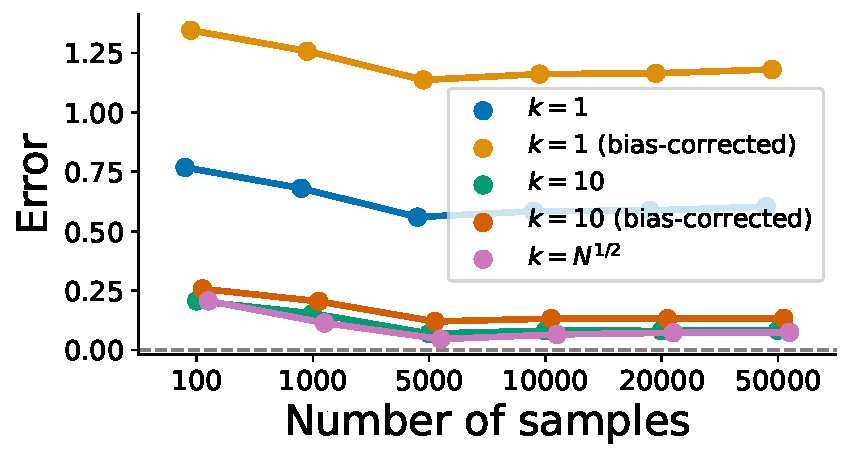
\includegraphics[width=.48\textwidth]{knnest-weak-corr-d=4-legend}}
	\subfloat[$d = 10$]{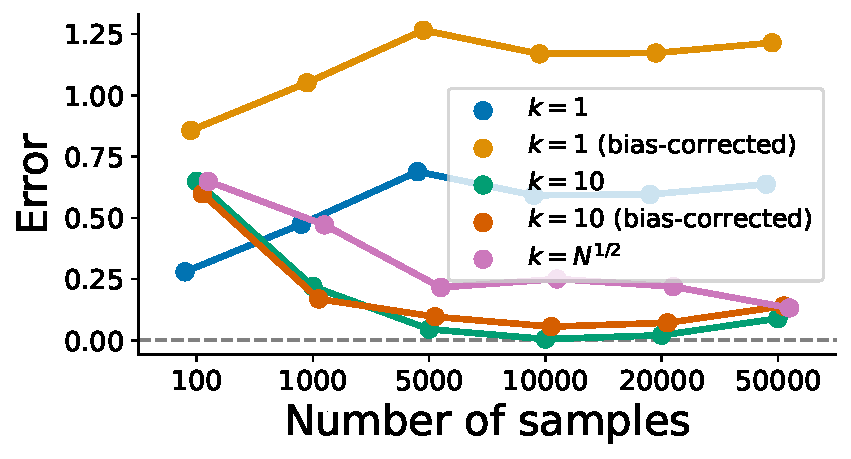
\includegraphics[width=.48\textwidth]{knnest-weak-corr-d=10-legend}}
	\\
	\subfloat[$d = 25$]{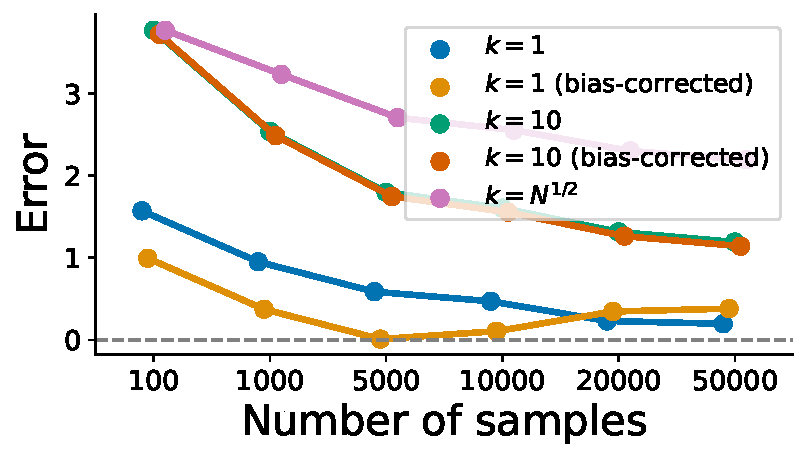
\includegraphics[width=.48\textwidth]{knnest-weak-corr-d=25-legend}}
	\subfloat[$d = 50$]{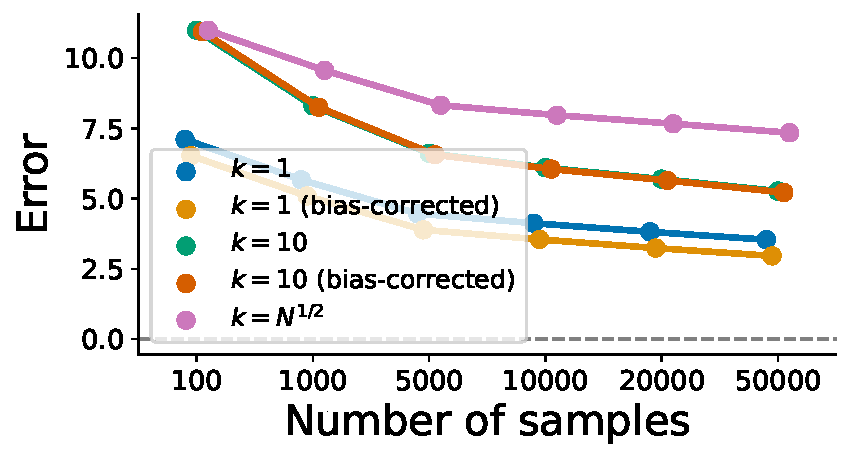
\includegraphics[width=.48\textwidth]{knnest-weak-corr-d=50-legend}}
	\caption{Absolute error against sample size for canonical $1$-nearest-neighbor estimator, canonical $10$-nearest-neighbor estimator, bias-corrected $1$-nearest-neighbor estimator, bias-corrected $10$-nearest-neighbor estimator and adaptive $k_{\numobs}$-nearest-neighbor estimator with $k_{\numobs}=\numobs^{1/2}$. Each panel corresponds with a different dimension $D\in\{4,10,25,50\}$. Gray dotted lines indicate no error.}
	\label{fig:knn-kl-est-comparison}
\end{figure}


\section{Checking \cref{assump:bounded-ratios}} \label{sec:checking-assumptions}

% We illustrate using a mixture of t-distributions and mixture of binomial distributions below.
%\begin{example}[Mixtures of t-distributions]
%\label{exa:t-dist}

\subsection{Mixture of t-distributions}
\label{appx:mixture-tdist-check}
	Consider the true data-generating distribution as a mixture of univariate t-distributions $P_{o}(\dee x)=\sum_{k = 1}^{\numcomps_{o}}\eta_{ok}F_{o}(\dee x; m_k, \tau_k, \nu)$ where the component density is 
    \[
    f_{o}(x;m,\tau, \nu) = \frac{\Gamma\left(\frac{\nu+1}{2}\right)}{\tau\sqrt{\nu \pi}\Gamma\left(\frac{\nu}{2}\right)}\left[\frac{\nu+\left(\frac{x-m}{\tau}\right)^2}{\nu}\right]^{-\left(\frac{\nu+1}{2}\right)}
    \]
    and $\Gamma(\cdot)$ is the gamma function. 
    Denote the asymptotic fitted Gaussian mixture model as $G_{\star}(\dee x) = \sum_{k=1}^{\numcomps}\eta_{\star k} F_{\star k}(\dee x)$,
    where $F_{\star k} = \distNorm(\mu_{\star k}, \sigma^2_{\star k})$. 
    %with density $f_{\star}(x; \mu, \sigma^2 )=\frac{1}{\sigma \sqrt{2\pi}}\exp\left(-\frac{1}{2}\left(\frac{x-\mu}{\sigma}\right)^2\right)$. 

    %Assume the degrees of freedom for $f_{o\ell}$ are equal for all $\ell$. 
    We want to show that $\sup_x\{ p_{\star}^{(\numcomps_{o})}(k \mid x)/p_{o}(k \mid x) \}< \infty$ when $\numcomps = \numcomps_{o}$.
	%It's easy to see $\eta_{\star k}/\eta_{ok} < \infty$. 
    Letting $\bar{\ell} = \argmax_\ell \sigma_{\star \ell}$, we have
	\begin{align}
		\sup_{x}\left\{\frac{p_{\star}^{(\numcomps_{o})}(k \mid x)}{p_{o}(k \mid x)}\right\}
		 & = \sup_{x}\left\{\frac{\eta^{(\numcomps_o)}_{\star k}f^{(\numcomps_o)}_{\star k}(x)}{g^{(\numcomps_o)}_{\star}(x)}\right\}\cdot \frac{p_{o}(x)}{\eta_{ok}f_{ok}(x)}    \\
		 & = \sup_{x}\left\{\frac{\eta^{(\numcomps_o)}_{\star k}}{\eta_{ok}} \cdot  \frac{f^{(\numcomps_o)}_{\star k}(x)}{\sum_{\ell=1}^{\numcomps_{o}}\eta^{(\numcomps_o)}_{\star \ell}f^{(\numcomps_o)}_{\star \ell}(x)} \cdot \frac{\sum_{\ell=1}^{\numcomps_{o}}\eta_{o\ell}f_{o\ell}(x)}{f_{ok}(x)}\right\} \\
         & < \frac{\eta^{(\numcomps_o)}_{\star k}\eta_{o\ell'}}{\eta_{ok}\eta^{(\numcomps_o)}_{\star \bar{\ell}}} \sup_{x} \left\{  \frac{f^{(\numcomps_o)}_{\star k}(x)}{f^{(\numcomps_o)}_{\star \bar{\ell}}(x)}\right\} \cdot  \sum_{\ell=1, \ell\ne k}^{\numcomps_o}\sup_{x}\left\{\frac{f_{o\ell}(x)}{f_{ok}(x)}\right\}. \label{eq:posterior-ratio}
	\end{align}
    Since $\sigma_{\star \bar{\ell}}$ is maximal, we can conclude that 
\begin{align}
\sup_{x} \left\{  \frac{f^{(\numcomps_o)}_{\star k}(x)}{f^{(\numcomps_o)}_{\star \bar{\ell}}(x)}\right\} = \sup_{x} \left\{ \frac{\sigma_{\star \bar{\ell}
}}{\sigma_{\star k}}\exp\left[\frac{1}{2} \left(\left(\frac{x-\mu_{\star \bar{\ell}}}{\sigma_{\star \bar{\ell}}}\right)^2 -\left(\frac{x-\mu_{\star k}}{\sigma_{\star k}}\right)^2 \right)\right] \right\} < \infty, \label{eq:sec-term}
\end{align}
and so it follows that 
\begin{align}
    \sum_{\ell=1, \ell\ne k}^{\numcomps_o}\sup_{x}\left\{\frac{f_{o\ell}(x)}{f_{ok}(x)}\right\} =  \sum_{\ell=1, \ell\ne k}^{\numcomps_o}\frac{\tau_{ok}}{\tau_{o\ell}} \sup_x \left\{ \left(\frac{\nu+\left(\frac{x-m_{o\ell}}{\tau_{o\ell}}\right)^2}{\nu+\left(\frac{x-m_{ok}}{\tau_{ok}}\right)^2}\right)^{-\left(\frac{\nu+1}{2}\right)} \right\} < \infty. \label{eq:third-term}
\end{align}
Plugging \cref{eq:sec-term,eq:third-term} back to \cref{eq:posterior-ratio} yields $\sup_x\{ p_{\star}^{(\numcomps_{o})}(k \mid x)/p_{o}(k \mid x) \}< \infty$ .


%The last term in \cref{eq:posterior-ratio} is the ratio between normal and t-distribution densities. For simplicity, we ignore the $k$-dependency in the densities and write
	% \begin{align}
	% 	\sup_x \frac{f(x; \mu,\sigma^2)}{f_{ok}(x; m, \tau, \nu)} = \frac{\tau}{\sigma}\cdot\frac{\Gamma\left(\frac{\nu}{2}\right)}{\Gamma\left(\frac{\nu+1}{2}\right)}\cdot\sqrt{\frac{\nu}{2}}\cdot \sup_x  \exp\left(-\frac{1}{2}\left(\frac{x-\mu}{\sigma}\right)^2\right) \cdot \left[\frac{\nu+\left(\frac{x-m}{\tau}\right)^2}{\nu}\right]^{\left(\frac{\nu+1}{2}\right)}. \label{eq:normal-t-ratio}
	% \end{align}
	% Observe that $\lim\limits_{\nu\rightarrow\infty}p_{o}(x; m, \tau, \nu) = f(x; m, \tau^2)$. The ratio in \cref{eq:normal-t-ratio} converges to $0$ for $\nu$ small and $|x|$ large.\PROBLEM{TODO(Jiawei): we want to be able to say that the $\sup$ over $x$ of the ratio of densities is finite.}

	% On the other hand, consider the ratio of mixture weights
	% \begin{align}
	% 	\frac{\eta^{(\numcomps_o)}_{\star k}}{\eta_{o}} = \frac{\int p^{(\numcomps_{o})}_{\star}(k\mid y)P_{o}(\dee y)}{\int p_{o}(k\mid y)P_{o}(\dee y)}
	% \end{align}
%\end{example}

%\begin{example}[Mixtures of negative binomial distributions]
\subsection{Mixture of bounded discrete distributions}

Suppose data are generated from a mixture of discrete distributions $P_{o}(\dee x)=\sum_{k = 1}^{\numcomps_{o}}\eta_{ok}F_{ok}(\dee x)$ with a finite support $\mathcal{X}$ for all $F_{ok}$. 
Denote the asymptotic fitted Poisson mixture model as $G_{\star}(\dee x) = \sum_{k=1}^{\numcomps}\eta_{\star k} F_{\star k}(\dee x)$, 
where $F_{\star k} = \distPoiss(\lambda_{\star k})$.
%$f_{\star}(x; \lambda)=\frac{\lambda^x e^{-\lambda}}{x!}$. 

To show $\sup_{x \in \mathcal{X}} \{p_{\star}^{(\numcomps_{o})}(k \mid x)/p_{o}(k \mid x)\} < \infty$ when $\numcomps = \numcomps_{o}$, we only need to show $\sup_{x} \left\{  f^{(\numcomps_o)}_{\star k}(x)/f^{(\numcomps_o)}_{\star \bar{\ell}(x)}\right\}<\infty$ and $ \sum_{\ell=1, \ell\ne k}^{\numcomps_o}\sup_{x}\left\{f_{o\ell}(x)/f_{ok}(x)\right\} < \infty$ according to \cref{eq:posterior-ratio}. Define $\bar{\ell} = \argmax_\ell \lambda_{\star \ell}$.  
Since $\lambda_{\star \bar{\ell}}$ is maximal, we can conclude that
    \begin{align}
\sup_{x} \left\{  \frac{f^{(\numcomps_o)}_{\star k}(x)}{f^{(\numcomps_o)}_{\star \bar{\ell}}(x)}\right\} = \sup_{x} \left\{ \left(\frac{\lambda_{\star k}}{\lambda_{\star \bar{\ell}}}\right)^x e^{-(\lambda_{\star \bar{\ell}} - \lambda_{\star k} )}\right\} < \infty. \label{eq:negbin-sec-term}
\end{align}
On the other hand, it follows by the finite support for $F_{ok}$ that 
\begin{align}
    \sum_{\ell=1, \ell\ne k}^{\numcomps_o}\sup_{x\in\mathcal{X}}\left\{\frac{f_{o\ell}(x)}{f_{ok}(x)}\right\} < \infty. \label{eq:neg-bin-third-term}
\end{align}
Combining \cref{eq:negbin-sec-term,eq:neg-bin-third-term} yields $\sup_x\{ p_{\star}^{(\numcomps_{o})}(k \mid x)/p_{o}(k \mid x) \}< \infty$.
%\end{example}

\section{Checking \cref{assump:sample_approx_able}}\label{sec:sample_approx_able_example}

We show that \cref{assump:sample_approx_able} holds for both the PMF models used for the experiments in \cref{sec:experiments}. 
% Although the assumption is stated in terms of the full sequence $y_{1:K}$, 
It is sufficient to verify the assumption for a single element $y_{nk}$ since the variance and integrability conditions can often be checked component-wise.
Hence, we drop the dependence on $n$ and $k$ in our notation. 

\subsection{Poisson PMF}

Consider the Poisson model with  $y \sim \distPoiss(\lambda)$ and $\lambda = W h$.
For convenience, we assume $h \sim \distGamma(\alpha, \beta)$.
%so
To compute the first and second moments of 
\[
  P(y\mid h) = \frac{(W h)^{y} e^{-W h}}{y!},
\]
we will use the identity
$\Gamma(z) = \int_0^\infty t^{z-1} e^{-t} \, \d t$ and integration by substitution.
For the first moment we have 
\begin{align}
\mathbb{E}_{h}\bigl[P(y\mid h)\bigr]
  &= \int_{0}^{\infty} \frac{(W h)^{y} e^{-W h}}{y!}
     \;\frac{\beta^{\alpha}}{\Gamma(\alpha)} h^{\alpha-1} e^{-\beta h} \, \mathrm{d}h\\[6pt]
  &= \frac{W^{y} \beta^{\alpha}}{y!\,\Gamma(\alpha)}
     \int_{0}^{\infty} h^{y+\alpha-1} e^{-(W+\beta)h} \, \mathrm{d}h\\[6pt]
  &= \frac{W^{y} \beta^{\alpha}\,\Gamma(y+\alpha)}{y!\,\Gamma(\alpha)(W+\beta)^{y+\alpha}},
\end{align}
while the second moment is 
\begin{align}
\mathbb{E}_{h}\bigl[P^{2}(y\mid h)\bigr]
  &= \int_{0}^{\infty} \frac{(W h)^{2y} e^{-2 W h}}{(y!)^{2}}
     \;\frac{\beta^{\alpha}}{\Gamma(\alpha)} h^{\alpha-1} e^{-\beta h} \, \mathrm{d}h\\[6pt]
  &= \frac{W^{2y} \beta^{\alpha}}{\Gamma(\alpha)(y!)^{2}}
     \int_{0}^{\infty} h^{2y+\alpha-1} e^{-(2W+\beta)h} \, \mathrm{d}h\\[6pt]
  &= \frac{W^{2y} \beta^{\alpha}\, \Gamma(2y+\alpha)}{\Gamma(\alpha)(y!)^{2}(2W+\beta)^{2y+\alpha}}.
\end{align}
% 
Taking the ratio of the second to the first moment, define 
\[
  C(y) = \frac{\mathbb{E}_{h}[P^{2}(y\mid h)]}{\mathbb{E}_{h}[P(y\mid h)]}
         = \frac{W^{y} \, \Gamma(2y+\alpha)}{y!\,\Gamma(y+\alpha)}
           \left(\frac{W+\beta}{2W+\beta}\right)^{y+\alpha}
           \cdot\left(\frac{1}{2W+\beta}\right)^{y},
\]
which is continuous and finite for all $y \in \nats$. 
Now, using Stirling's approximation
$ \Gamma(z) \sim \sqrt{2\pi}\, z^{z-1/2} e^{-z},$ we have
\begin{align}
    \frac{\Gamma(2y+\alpha)}{y!\,\Gamma(y+\alpha)} &\sim
    \frac{(2y)^{2y+\alpha-1/2} e^{-2y}}{\sqrt{2\pi}\,y^{y+\alpha-1/2} e^{-y}\cdot \sqrt{2\pi}\,y^{y+1/2} e^{-y}}
    \sim \frac{2^{2y+\alpha}}{\sqrt{\pi y}}.
\end{align}
Substituting into $C(y)$ yields
\begin{align}
C(y)
 &\sim \frac{W^{y}}{\sqrt{\pi y}}
        \left(\frac{W+\beta}{2W+\beta}\right)^{\alpha}
        \left(\frac{W+\beta}{2W+\beta}\right)^{y}
        \left(\frac{1}{2W+\beta}\right)^{y}
        2^{2y}\\
 &\sim \frac{1}{\sqrt{\pi y}}
        \left(\frac{W+\beta}{2W+\beta}\right)^{\alpha}
        \left(\frac{2^2W(W+\beta)}{(2W+\beta)^2}\right)^{y}\\
 &\sim \frac{1}{\sqrt{\pi y}}
        \left(\frac{4W^2+4W\beta}{4W^2+\beta^2+4W\beta}\right)^{y}.      
\end{align}
Because $0<\frac{4W^2+4W\beta}{4W^2+\beta^2+4W\beta} < 1$, the ratio $C(y)$ decays exponentially as $y \to \infty$, 
hence $\sum_{y=0}^{\infty} C(y)  <\infty$.

\subsection{Gaussian PMF}

Consider the Gaussian setting $y \sim \mathcal{N}(\phi h, \sigma^2)$
and, following common practice, we let $h \sim \mathcal{N}(\mu, \tau^2)$. 
To compute the moments of $p(y \mid h)$, we integrate over the latent variable $h$ by combining the terms in the exponential, completing the square, and using the Gaussian integral identity
$\int_{-\infty}^{\infty} e^{-(a x^2 + b x + c)} \, \dee x = \sqrt{\frac{\pi}{a}} e^{\frac{b^2}{4a} - c}.$ 
The first moment is 
% 
\begin{align}
\mathbb{E}_h [p(y \mid h)] 
&= \int_{-\infty}^{\infty} \frac{1}{\sqrt{2\pi\sigma^2}} \exp\left(-\frac{(y - \phi h)^2}{2\sigma^2} \right)
\cdot \frac{1}{\sqrt{2\pi\tau^2}} \exp\left(-\frac{(h - \mu)^2}{2\tau^2} \right) \, dh \\
&\propto \exp\left\{ -\frac{(y - \phi \mu)^2}{2(\phi^2 \tau^2 + \sigma^2)} \right\},
\end{align}
while the second moment is 
% also the moment
\begin{align}
\mathbb{E}_h [p(y \mid h)^2] 
&= \int_{-\infty}^{\infty} \left( \frac{1}{\sqrt{2\pi\sigma^2}} \exp\left(-\frac{(y - \phi h)^2}{2\sigma^2} \right) \right)^2
\cdot \frac{1}{\sqrt{2\pi\tau^2}} \exp\left(-\frac{(h - \mu)^2}{2\tau^2} \right) \, dh \\
&\propto \exp\left\{ -\frac{(y - \phi \mu)^2}{2(\phi^2 \tau^2 + \frac{1}{2}\sigma^2)} \right\}.
\end{align}
Therefore, up to a multiplicative constant, the ratio of moments is 
\begin{align}
    C(y) 
    &= \frac{\mathbb{E}_{h}[P^{2}(y\mid h)]}{\mathbb{E}_{h}[P(y\mid h)]} \\
    &\propto \frac{ \exp\left\{ -\frac{(y - \phi \mu)^2}{2(\phi^2 \tau^2 + \frac{1}{2}\sigma^2)} \right\} }{ \exp\left\{ -\frac{(y - \phi \mu)^2}{2(\phi^2 \tau^2 + \sigma^2)} \right\} }\\
    % &= \exp\left\{ -\frac{(y - \phi \mu)^2}{2(\phi^2 \tau^2 + \frac{1}{2}\sigma^2)} + \frac{(y - \phi \mu)^2}{2(\phi^2 \tau^2 + \sigma^2)} \right\} \\
    &= \exp\left\{ -(y - \phi \mu)^2 \left( \frac{1}{2(\phi^2 \tau^2 + \frac{1}{2}\sigma^2)} - \frac{1}{2(\phi^2 \tau^2 + \sigma^2)} \right) \right\}.
\end{align}
Since $\frac{1}{2(\phi^2 \tau^2 + \frac{1}{2}\sigma^2)} > \frac{1}{2(\phi^2 \tau^2 + \sigma^2)}$, 
we get $C(y) \propto \exp\left\{ -a (y - \phi \mu)^2 \right\}$ for some $a > 0$. Therefore,
$C(y)$ decays exponentially as $y \to \infty$ and hence $\int C(y)\d y <\infty$.  


\section{Limitations of Coarsening}

\PROBLEM{XXX: maybe remove?}

The following toy example illustrates how coarsening and the Bayesian information criterion can overfit even in scenarios with only a modest degree of misspecification.
%\begin{example}[Illustration: Overfitting the Number of Mixture Model Components]
	% Finding $\numcomps_{o}$ can be challenging for standard model selection approaches given the presence of model misspecification \citep{Cai:2021,Guha:2021,Fruhwurth:2006,Miller:2019}.
	% Specifically, as the number of observations increases, model selection criteria tend to create additional clusters to compensate for the model--data mismatch and thus overestimates
	% $\numcomps_{o}$.

	%do not always provide robust model selection consistency.
	We generate data from a mixture of $\numcomps_{o} = 2$ skew normal distributions but fit the data using a Gaussian mixture.
	The level of misspecification is controlled by the skewness parameter of each skew normal component in the true generative distribution $P_{o}$.
	We consider the following scenarios: two equal-sized clusters with the same level of misspecification (denoted \texttt{same})
	and two equal-sized clusters with different levels of misspecification (denoted \texttt{different}).
	See \cref{sec:high-dim-simulation} for further details about the experimental set-up.
	%\begin{enumerate}[(i)]
	%	%	\item \label{eg:s1} two equal-sized clusters with no misspecification;
	%	\item \label{eg:s2}two equal-sized clusters with the same level of misspecification;
	%	\item \label{eg:s3} two equal-sized clusters with different levels of misspecification.
	%	%	\item \label{eg:s4} two different-sized clusters with same level of misspecification.
	%\end{enumerate}
	As shown in the first row of \cref{fig:motivate-comparison}, in both scenarios using expectation--maximization (EM)
	with the Bayesian information criterion (BIC) results in estimating $\numcomps \gg \numcomps_{o}$
	to capture the skewness of each component.
	As shown in the second row of \cref{fig:motivate-comparison},
	the coarsened posterior performs well in the \texttt{same} case but overfits the cluster with a larger degree of misspecification in the \texttt{different} scenario.
	% its limitations become evident when the degree of misspecification differs significantly between components.
	% In the , the coarsened posterior overfits the cluster with a larger degree of misspecification.
	%the coarsened posterior \citep{Miller:2019}, and EM with our proposed model selection criterion.
	%Depending on the comparable sizes and levels of misspecification between components, the candidate inferences perform differently. We discuss the setup parameters with more detail in  
	% % as number of observations increases. 
	% %Such overfitting phenomena raise severe concern about existing inference on the identification about the correct number of latent types with finite mixture models, when model is ill-defined.
	% %\end{example}
	% While the coarsened posterior  performs well in the \texttt{same} case,
	% some limitations become evident when the degree of misspecification differs significantly between components.
	% In the \texttt{different} scenario, the coarsened posterior overfits the cluster with a larger degree of misspecification.
	% %This limitation arises from applying robustness at the overall model level.
	% %, which leads to a roughly even distribution of this robustness across each component. 
	% %In \cref{sec:simulation-gauss}, we also that the coarsened posterior generally fails to capture $\numcomps_{o}$ when components are of relatively different degrees of misspecification scaled by component size. =	
%\end{example}


\begin{figure}[tp]
	\centering
	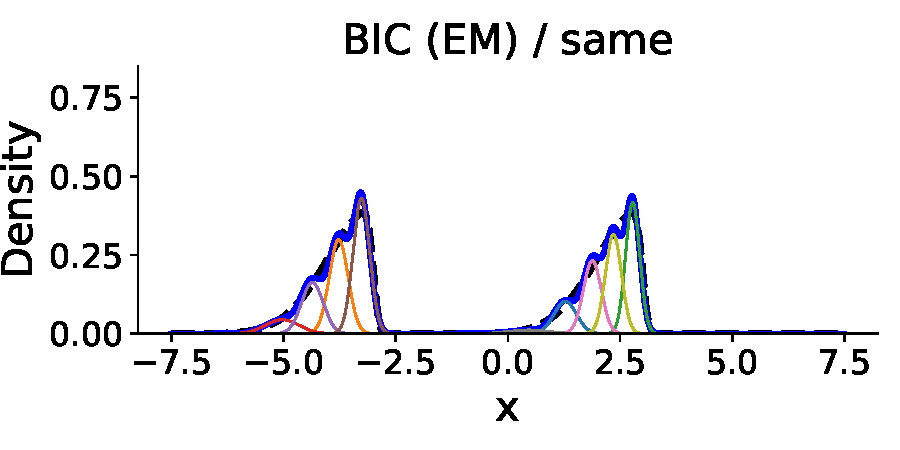
\includegraphics[width=.48\textwidth]{em-pdfs-n=5000-close-False-rsize-equal-rmis-equal}
	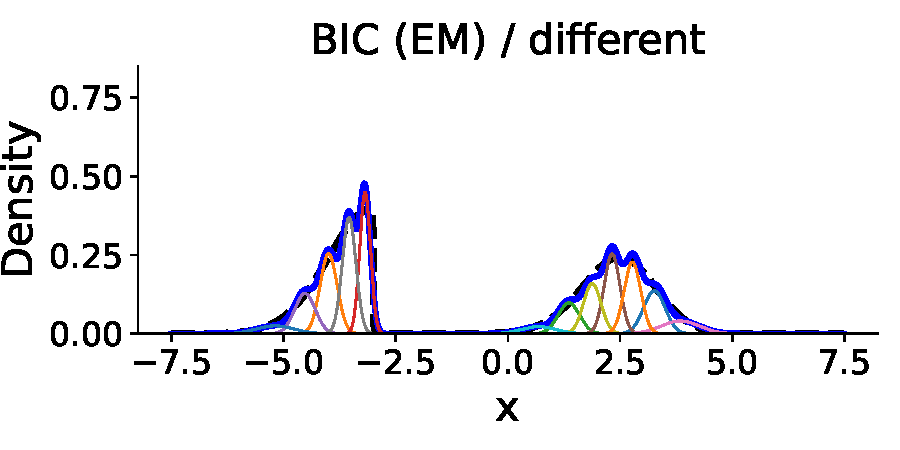
\includegraphics[width=.48\textwidth]{em-pdfs-n=10000-close-False-rsize-equal-rmis-bbig-small}\\
	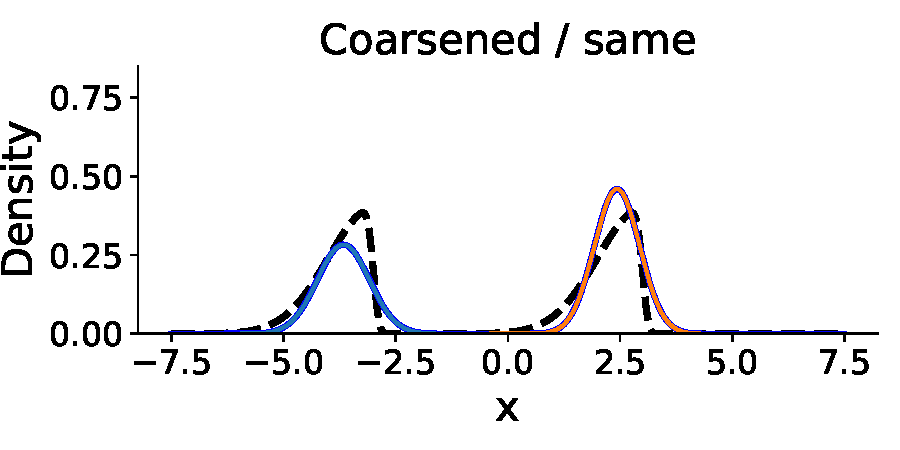
\includegraphics[width=.48\textwidth]{skewnorm-coarsen-pdfs-n=5000-close-False-rsize-equal-rmis-equal}
	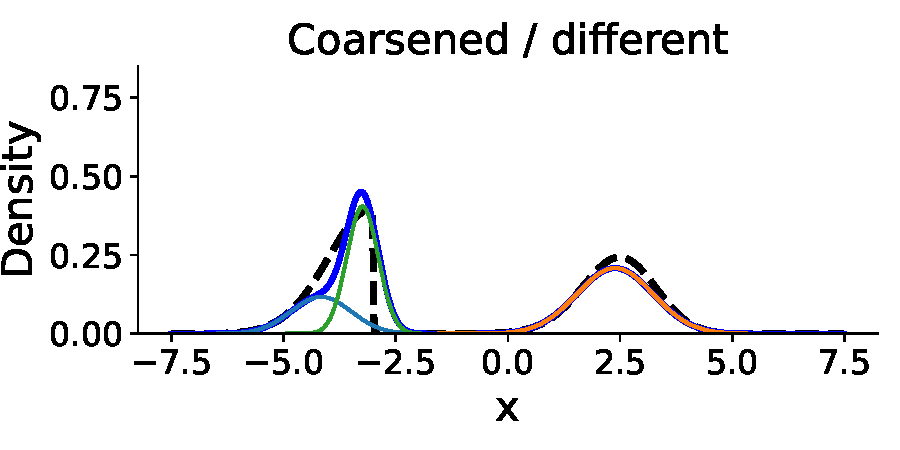
\includegraphics[width=.48\textwidth]{skewnorm-coarsen-pdfs-n=10000-close-False-rsize-equal-rmis-bbig-small}\\
	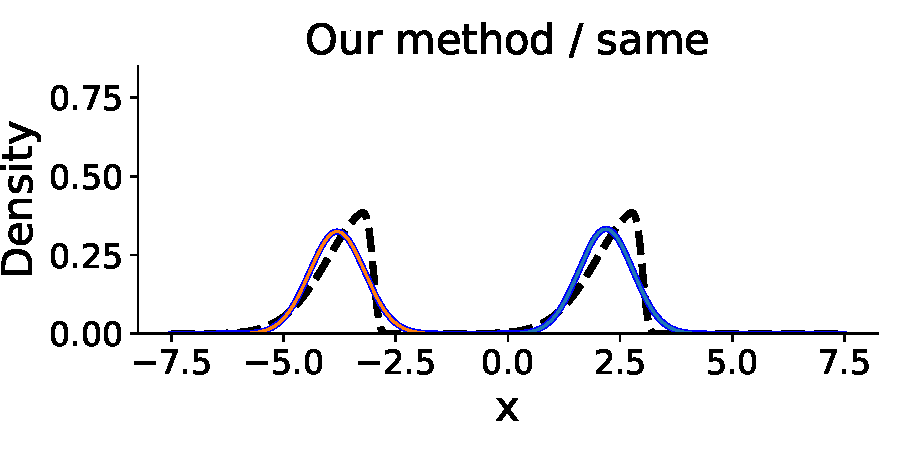
\includegraphics[width=.48\textwidth]{skewnorm-stare-pdfs-n=5000-close-False-rsize-equal-rmis-equal}
	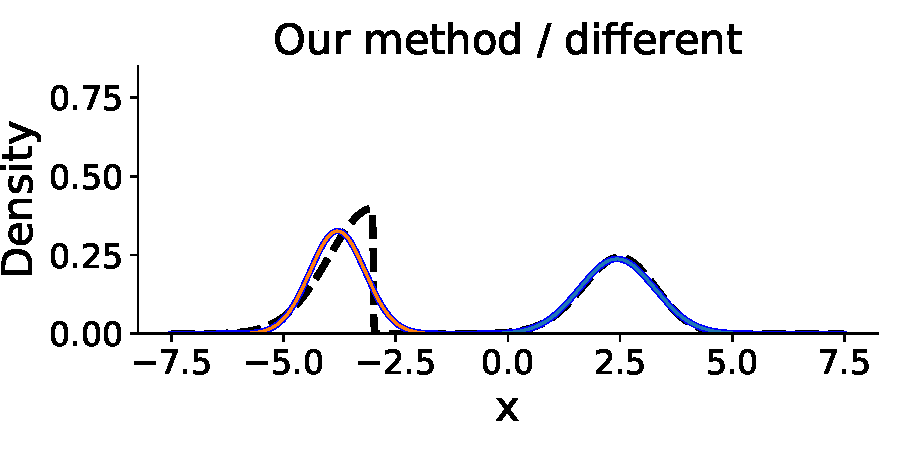
\includegraphics[width=.48\textwidth]{skewnorm-stare-pdfs-n=10000-close-False-rsize-equal-rmis-bbig-small}
	\caption{
		For the mixture of skew-normals example from \cref{sec:intro},
		each panel shows the density of $P_{o}$ (dashed lines) and the densities of the fitted Gaussian mixture model and each
		component distribution (solid lines) using $\numobs = 10\,000$ observations.
		The ``same'' and ``different'' scenarios describes the relative degree of misspecification of the two components.
		Results are given for three approaches:
		expectation--maximization with the Bayesian information criterion (first row),
		the coarsened posterior (second row),
		and our robust model selection method (third row).}
	\label{fig:motivate-comparison}
\end{figure}


\section{Additional Calibration Figures}

\subsection{Simulation Study}
\label{appx:simulation-gauss}

The coarsened posterior requires calibration of the hyperparameter $\alpha$, which determines the degree of misspecification.
We select $\alpha$ using the \emph{elbow method} proposed by \citet{Miller:2019}.
In this section, we include all calibration figures for the coarsened posterior following the code provided by \citet{Miller:2019}.

As shown in \cref{fig:coarsen-calibration}, we set $\alpha$ based on the turning point where we see no significant increase
in the log-likelihood if $\alpha$ increases further.
Using these values for $\alpha$, we can see for all cases except the \texttt{small-large} case, the coarsened posterior consistently estimates the number of clusters (after removing mini clusters with size $<2\%$) as $\widehat{\numcomps} = 3 > \numcomps_{o} = 2$.

\begin{figure}[tp]
	\centering
	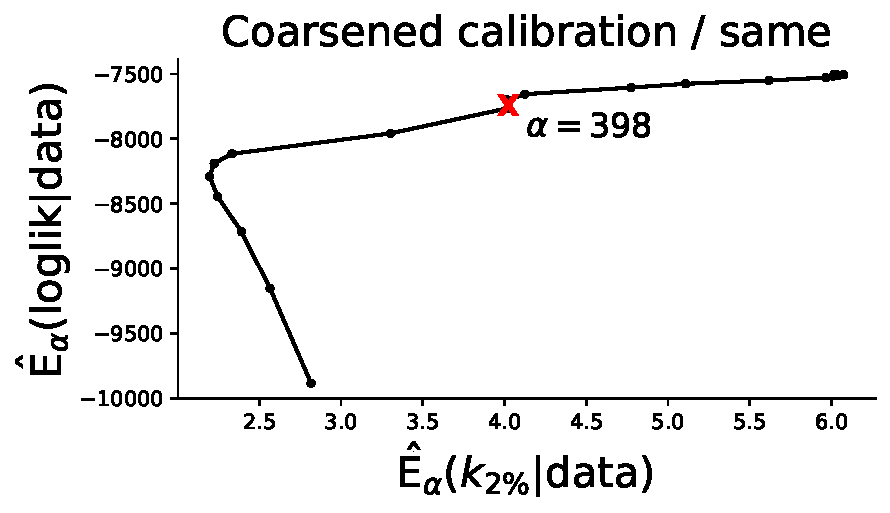
\includegraphics[width=.48\textwidth]{skewnorm-coarsen-calibration-n=5000-close-False-rsize-equal-rmis-equal}
	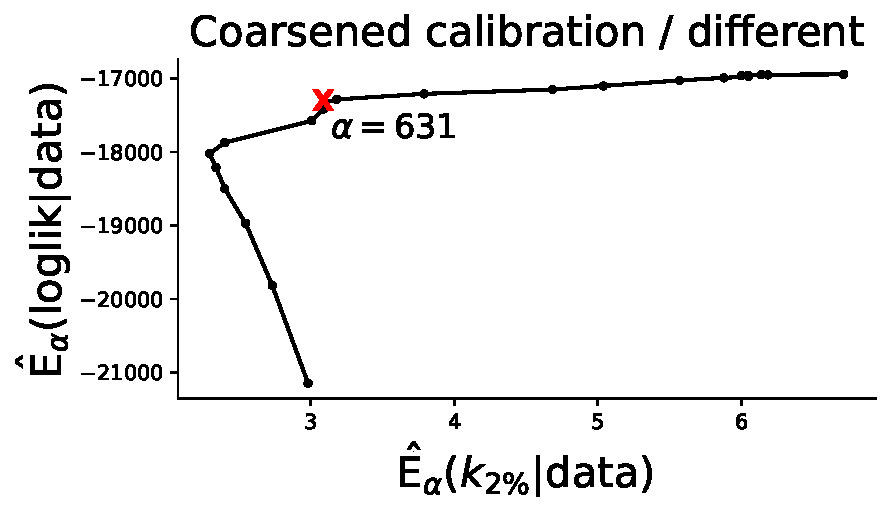
\includegraphics[width=.48\textwidth]{skewnorm-coarsen-calibration-n=10000-close-False-rsize-equal-rmis-bbig-small}\\
	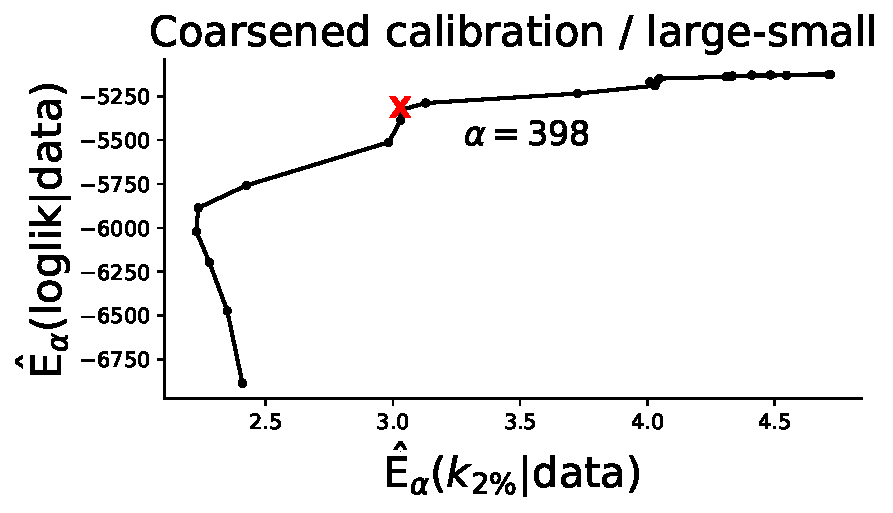
\includegraphics[width=.48\textwidth]{skewnorm-coarsen-calibration-n=5000-close-False-rsize-big-small-rmis-big-small}
	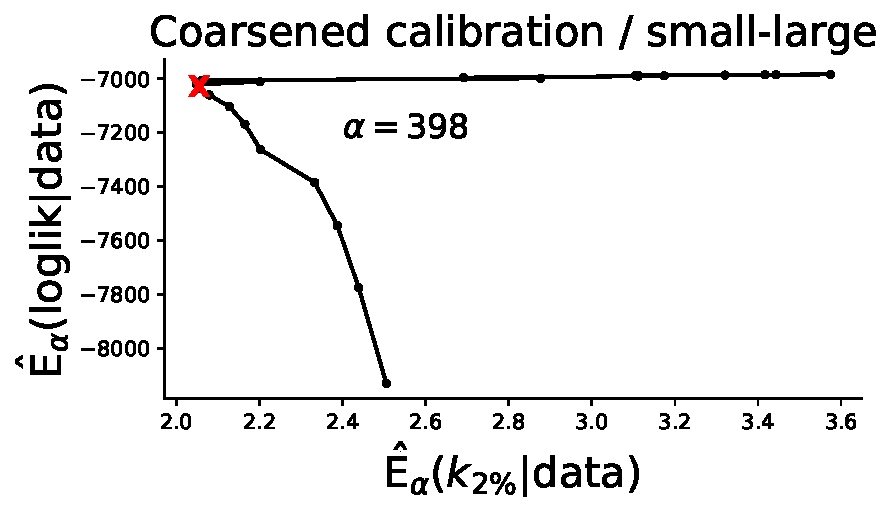
\includegraphics[width=.48\textwidth]{skewnorm-coarsen-calibration-n=5000-close-False-rsize-big-small-rmis-small-big}\\
	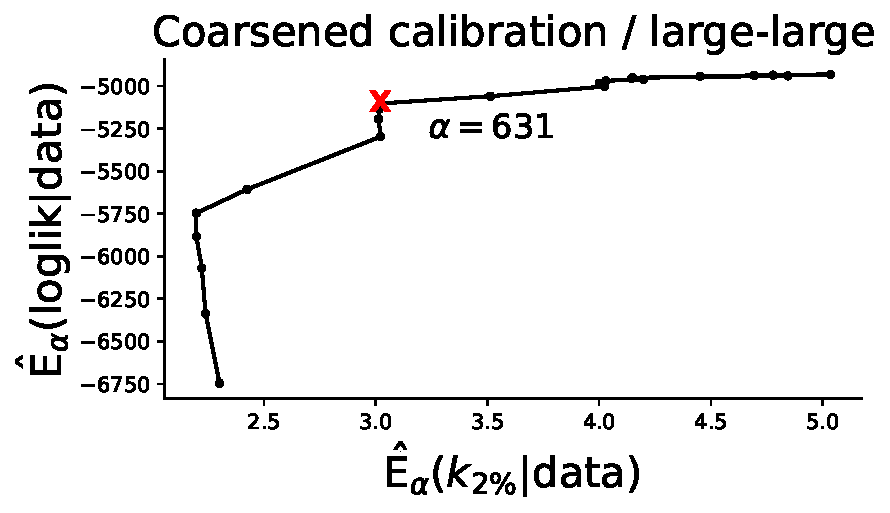
\includegraphics[width=.48\textwidth]{skewnorm-coarsen-calibration-n=5000-close-False-rsize-big-small-rmis-equal}
	\caption{For the mixture of skew normals experiments from \cref{sec:intro,sec:high-dim-simulation}, each panel shows the expected log-likelihood $\widehat{E}_{\alpha}(\mathrm{loglik}\mid \mathrm{data})$ against the expected number of clusters which excludes tiny clusters of size less that $2\%$ of whole dataset denoted as $\widehat{E}_{\alpha}(k_{2\%}\mid \mathrm{data})$.
		We select $\alpha$ as the elbow point in the plots.}
	\label{fig:coarsen-calibration}
\end{figure}

\subsection{Flow Cytometry Data}
\label{appx:flow-cytometry}

In this section, we include loss and F-measure plots of our model selection method on all test datasets 7--12.
See \citet[Section 5.2]{Miller:2019} for a discussion of the exact calibration procedure for the coarsened posterior.
% on flow cytometry datasets and recommend users to refer to .

Recall that to calibrate $\rho$, we select $\rho$ that optimizes the F-measure across first $6$ datasets.
To incorporate this prior knowledge on test datasets, we suggests selecting the value of $\numcomps$
that has has stable penalized loss and is closest to the optimal $\rho$.
We compare our selection $\widehat{\numcomps}$ with the ground truth $\numcomps_o$ labeled by experts.
For each dataset, there is always one cluster labeled as unknown due to some unclear information for cells.
With automatic clustering algorithm, it is natural for the algorithm to identify those unlabeled points and assign them to other clusters, which results in $\numcomps_o-1$ clusters.
So we treat both $\numcomps_o$ and $\numcomps_o-1$ as ground truth in our analysis.
As shown in \cref{fig:GvHD,fig:GvHD2}, our selection method results in highest F-measure for datasets 8--12.
Dataset 7 is challenging and even the ground truth does not produce a large F-measure.




\begin{figure}[tp]
	\centering
	\subfloat[Data 7]{\label{fig:data7}
		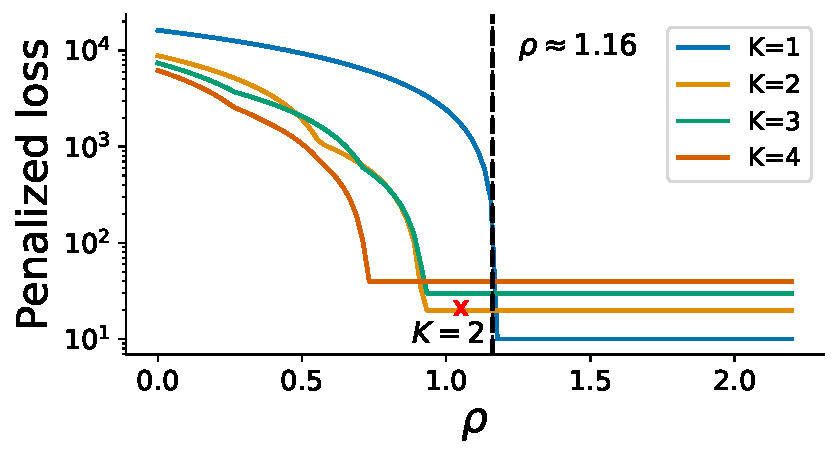
\includegraphics[width=.48\textwidth]{GvHD7-loss-plot-legend}
		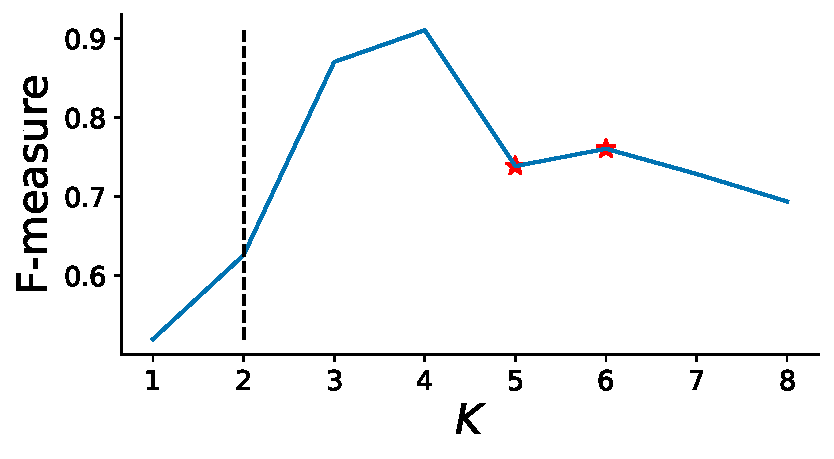
\includegraphics[width=.48\textwidth]{GvHD7-fmeasure-plot}}	\\
	\subfloat[Data 8]{\label{fig:data8}
		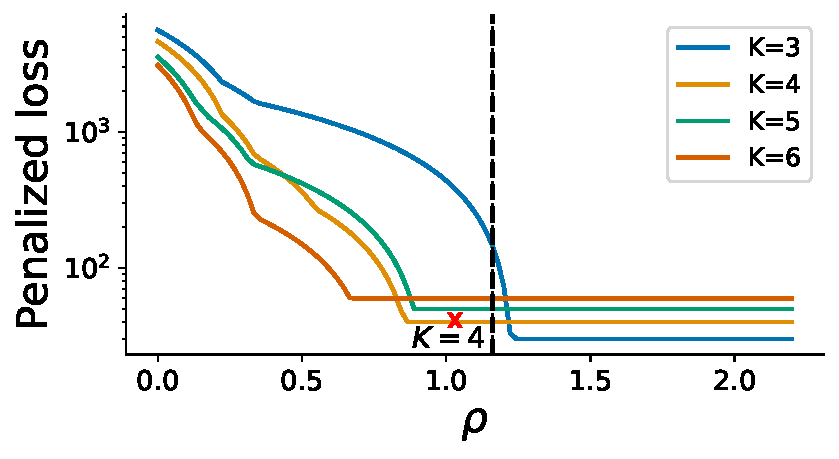
\includegraphics[width=.48\textwidth]{GvHD8-loss-plot-legend}
		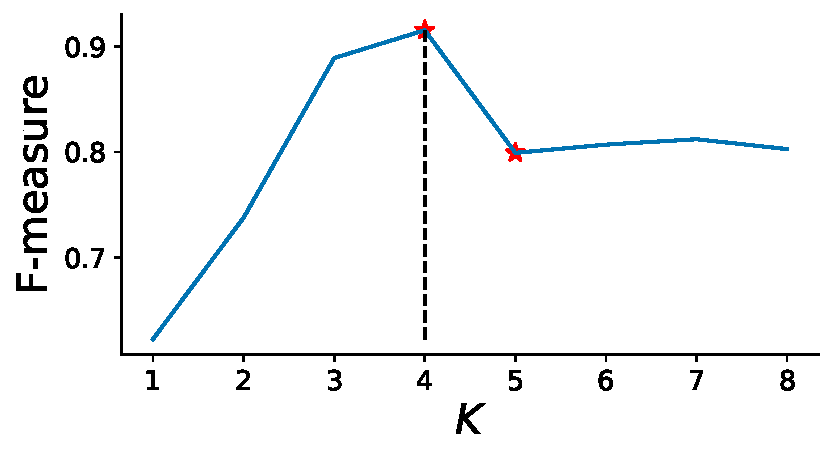
\includegraphics[width=.48\textwidth]{GvHD8-fmeasure-plot}}	\\
	\subfloat[Data 9]{\label{fig:data9}
		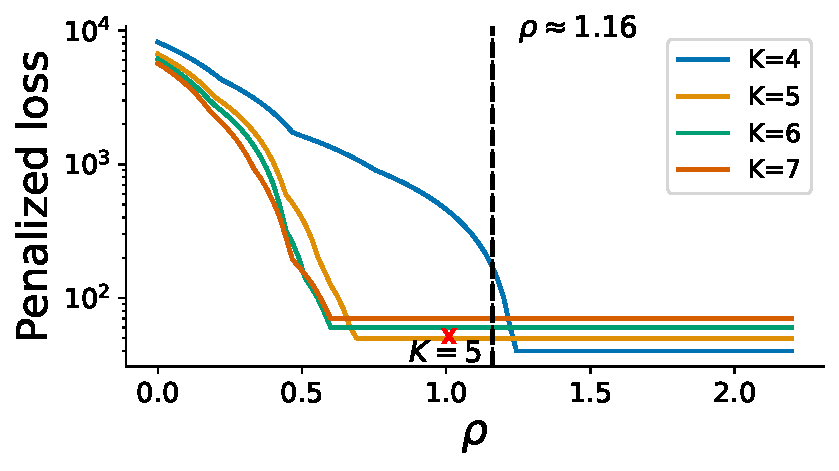
\includegraphics[width=.48\textwidth]{GvHD9-loss-plot-legend}
		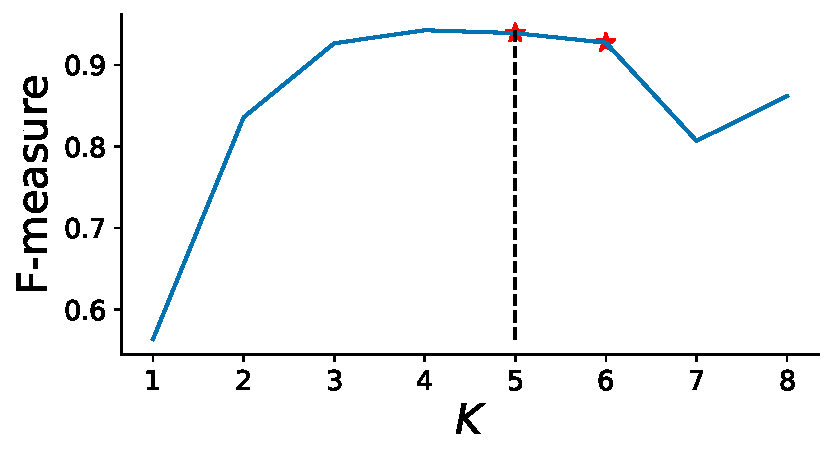
\includegraphics[width=.48\textwidth]{GvHD9-fmeasure-plot}}
	\caption{Calibration and F-measure plots for test datasets 7--9 in flow cytometry experiments. \textbf{Left}: The black dashed lines indicate the optimal $\rho$ calibrated on training datasets 1--6. The cross mark indicates the selection for number of clusters. \textbf{Right}: F-measure against the number of clusters. The dashed line shows the number of clusters selected by \methodname and the red star indicates the ground truth $\numcomps_{o}$.}
	\label{fig:GvHD}
\end{figure}


\begin{figure}[tp]
	\centering
	\subfloat[Data 10]{\label{fig:data10}
		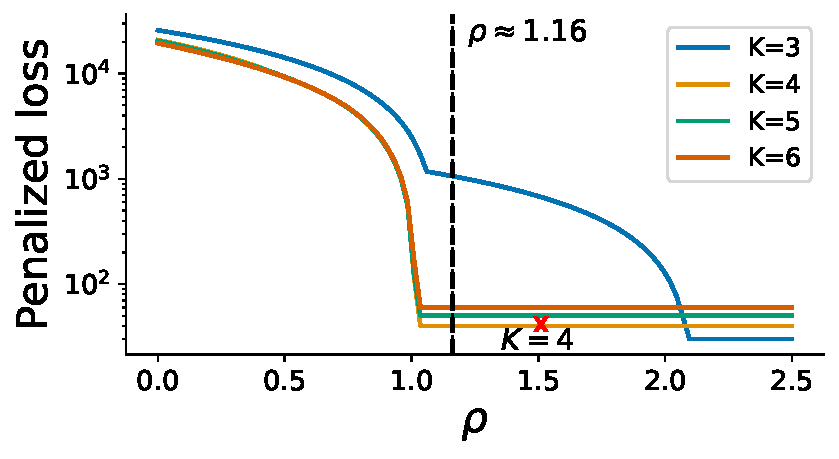
\includegraphics[width=.48\textwidth]{GvHD10-loss-plot-legend}
		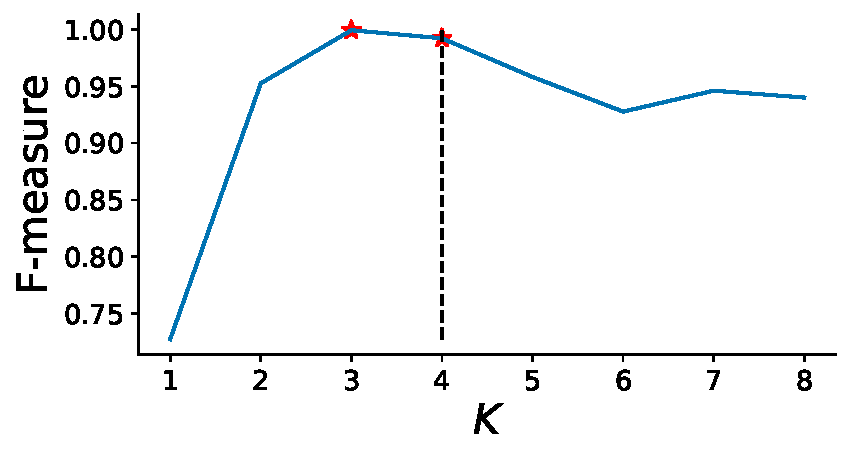
\includegraphics[width=.48\textwidth]{GvHD10-fmeasure-plot}}	\\
	\subfloat[Data 11]{\label{fig:data11}
		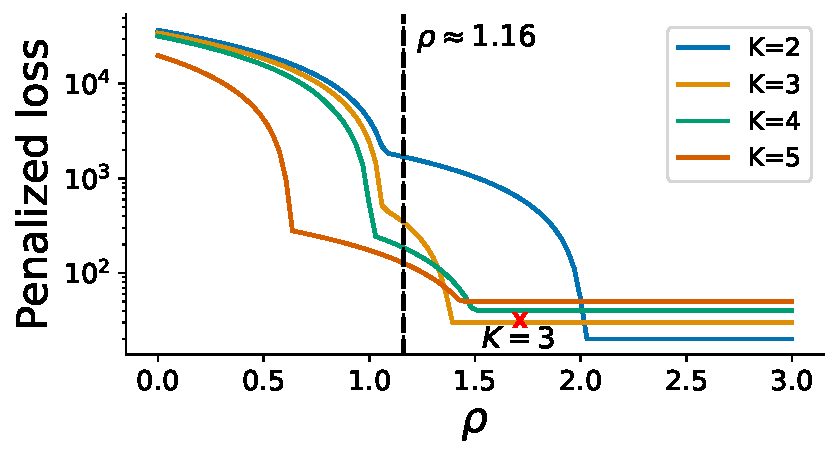
\includegraphics[width=.48\textwidth]{GvHD11-loss-plot-legend}
		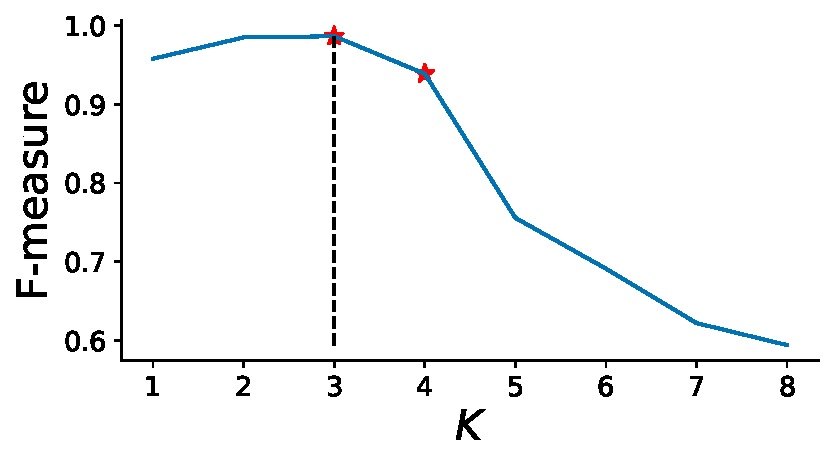
\includegraphics[width=.48\textwidth]{GvHD11-fmeasure-plot}}	\\
	\subfloat[Data 12]{\label{fig:data12}
		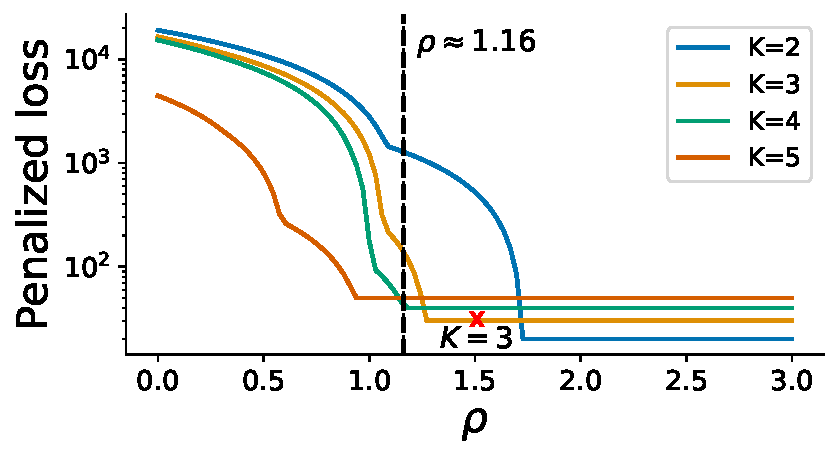
\includegraphics[width=.48\textwidth]{GvHD12-loss-plot-legend}
		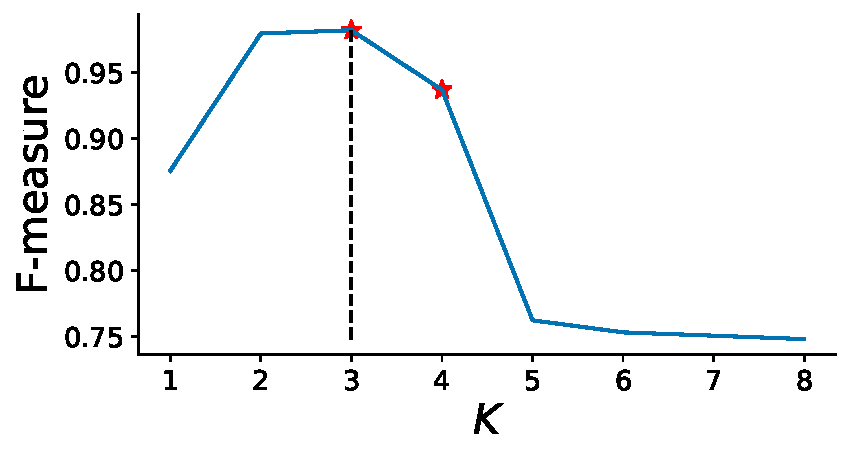
\includegraphics[width=.48\textwidth]{GvHD12-fmeasure-plot}}
	\caption{Calibration and F-measure plots for test datasets $10-12$ in flow cytometry experiments. See caption for \cref{fig:GvHD} for details}
	\label{fig:GvHD2}
\end{figure}




\begin{figure}[tp]
	\centering
	\subfloat[Data 7, $\numcomps=8$]{\label{fig:data7-loss}
		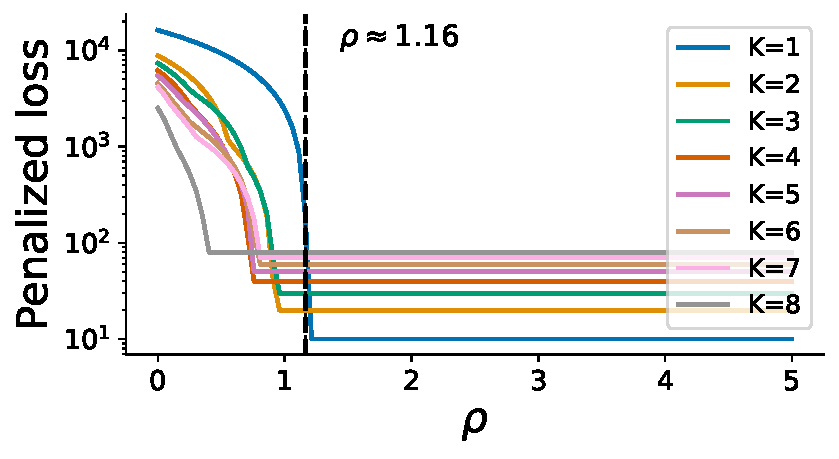
\includegraphics[width=.48\textwidth]{GvHD7-all-loss-plot-legend}}
	\subfloat[Data 8, $\numcomps=7$]{\label{fig:data8-loss}
		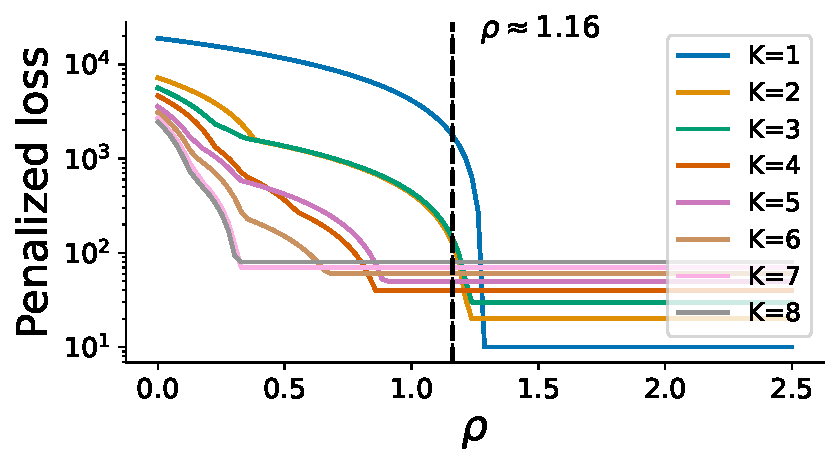
\includegraphics[width=.48\textwidth]{GvHD8-all-loss-plot-legend}}\\
	\subfloat[Data 9, $\numcomps=5$]{\label{fig:data9-loss}
		\includegraphics[width=.48\textwidth]{GvHD9-all-loss-plot-legend}}
	\subfloat[Data 10, $\numcomps=4$]{\label{fig:data10-loss}
		\includegraphics[width=.48\textwidth]{GvHD10-all-loss-plot-legend}}\\
	\subfloat[Data 11, $\numcomps=3$]{\label{fig:data11-loss}
		\includegraphics[width=.48\textwidth]{GvHD11-all-loss-plot-legend}}
	\subfloat[Data 12, $\numcomps=3$]{\label{fig:data12-loss}
		\includegraphics[width=.48\textwidth]{GvHD12-all-loss-plot-legend}}
	\caption{Calibration including $\numcomps=1,\ldots,8$ for test datasets 7--12 in flow cytometry experiments. }
	\label{fig:GvHD3}
\end{figure}



\section{Skew-normal Mixture Simulation Study}
\label{sec:simulation-gauss}

%We now provide further details about the motivating example in \cref{sec:motivation}, and illustrate
%that \methodname selects the correct number of components under a variety of conditions on the level of misspecification
%and the relative sizes of the mixture components.
%%To show the strength of structurally aware robust inference in the context of model misspecification, 
%We generate data $x_1, \ldots, x_n \in \mathbb{R}$ from skew-normal mixtures of the form $P_{o} = \sum_{k=1}^{\numcomps_{o}}\eta_{ok}\distSNorm(\mu_{ok}, \sigma_{ok},\gamma_{ok})$, where $\distSNorm(\cdot)$ denotes the skew-normal distribution and $\gamma_{ok}$ denotes the skewness parameter.
%The density of the skew-normal distribution $\distSNorm(\mu, \sigma,\gamma)$ is $f(x) = 2\phi(x;\mu,\sigma)\Phi(\gamma x;\mu,\sigma)$, where $\phi(x;\mu,\sigma)$ and $\Phi(x;\mu,\sigma)$ denote the probability density function and the cumulative distribution function of $\distNorm(\mu,\sigma)$ respectively.
%We model the data using  Gaussian mixture model $G_{\allparam} = \sum_{k=1}^{\numcomps}\eta_{k}\distNorm(\mu_{k}, \sigma_{k})$.
%The bigger $|\gamma_{ok}|$, the larger the deviation from the Gaussian distribution,
%hence introducing a higher degree of misspecification.

In \cref{sec:intro}, we consider the case of two clusters of equal size. 
We set $\eta_{o} = (0.5, 0.5)$, $\mu_{o} = (-3,3)$, and $\sigma_{o} = (1,1)$ for the two scenarios in \cref{fig:motivate-comparison}: $\gamma_o = (-10,-1)$ (denoted \texttt{different}) and $\gamma_o = (-10,-10)$ (denoted \texttt{same}).
We now compare \methodname to the coarsened posterior with data from
two-component mixtures of different cluster sizes. %, under which coarsened posterior fails. 
%The degree of misspecification is controlled by distributional parameters $\allparam_o = (\mu_{o}, \sigma_{o}, \gamma_{o})$. 
We set $\eta_{o} = (0.95, 0.05)$, $\mu_{o} = (-3,3)$, and $\sigma_{o} = (1,1)$ for the following three scenarios:
$\gamma_o = (-10,-1)$ (denoted \texttt{large-small}),  $\gamma_o = (-1,-10)$ (denoted \texttt{small-large}),
and  $\gamma_o = (-10,-10)$ (denoted \texttt{large-large}).

\begin{figure}[tp]
	\centering
	\subfloat{\label{fig:gauss-cpos-pdfs-1}\includegraphics[width=.32\textwidth]{skewnorm-coarsen-pdfs-n=5000-close-False-rsize-big-small-rmis-big-small}}
	\subfloat{\label{fig:gauss-cpos-pdfs-2}\includegraphics[width=.32\textwidth]{skewnorm-coarsen-pdfs-n=5000-close-False-rsize-big-small-rmis-small-big}}
	\subfloat{\label{fig:gauss-cpos-pdfs-3}\includegraphics[width=.32\textwidth]{skewnorm-coarsen-pdfs-n=5000-close-False-rsize-big-small-rmis-equal}}
	\\
	\subfloat{\label{fig:gauss-stare-pdfs-1}\includegraphics[width=.32\textwidth]{skewnorm-stare-pdfs-n=5000-close-False-rsize-big-small-rmis-big-small}}
	\subfloat{\label{fig:gauss-stare-pdfs-2}\includegraphics[width=.32\textwidth]{skewnorm-stare-pdfs-n=5000-close-False-rsize-big-small-rmis-small-big}}
	\subfloat{\label{fig:gauss-stare-pdfs-3}\includegraphics[width=.32\textwidth]{skewnorm-stare-pdfs-n=5000-close-False-rsize-big-small-rmis-equal}}
	\\
	\subfloat{\label{fig:gauss-stare-penloss-1}\includegraphics[width=.32\textwidth]{skewnorm-stare-loss-n=5000-close-False-rsize-big-small-rmis-big-small-legend}}
	\subfloat{\label{fig:gauss-stare-penloss-2}\includegraphics[width=.32\textwidth]{skewnorm-stare-loss-n=5000-close-False-rsize-big-small-rmis-small-big-legend}}
	\subfloat{\label{fig:gauss-stare-penloss-3}\includegraphics[width=.32\textwidth]{skewnorm-stare-loss-n=5000-close-False-rsize-big-small-rmis-equal-legend}}


	\caption{
		Comparison between the coarsened posterior and \methodname when using a Gaussian mixture model to fit data generated from a mixture of
		skew-normal distributions.
		\textbf{First row:} Densities of the model and components selected using the coarsened posterior (solid lines) and the density of the data distribution (dashed line). The title specifies the data-generating distribution and the number of components selected.
		In the middle plot of the first row, the minor cluster contains two components.
		\textbf{Second row:} Densities of the model and components selected using our structurally aware robust method.
		\textbf{Third row:} Penalized loss plots, where the cross mark indicates the first wide stable region and is labeled with the number of clusters \methodname selects.
		Line colors correspond to different $\numcomps$ values.}
	\label{fig:gauss-simulation}
\end{figure}

For the coarsened posterior, we calibrate the hyperparameter $\alpha$ following the procedure from \citet[Section 4]{Miller:2019}.
First, we use Markov chain Monte Carlo to approximate the coarsened posterior for $\alpha$ values ranging from $10$ to $10^5$.
Then, we select the coarsened posterior with the $\alpha$ value at the clear cusp that indicates a good fit and low complexity.
See the Supplementary Materials for further details and calibration plots.
%We then use the proposed $\alpha$ in the coarsening method to do inference for the same dataset. \PROBLEM{(1) For all experiments, we should include calibration plots for coarsened posterior and \methodname in the SM. It's OK if this results in some duplication.  }
%As shown in \cref{fig:gauss-simulation}, coarsened posterior fails in different ways. For Scenarios (\ref{gaussmix-s1}) and (\ref{gaussmix-s3}), the coarsened posterior tend to overfit the larger cluster. 
%For Scenario (\ref{gaussmix-s2}), the smaller cluster with more misspecification is underfit.
As shown for \texttt{large-small} and \texttt{large-large} in \cref{fig:gauss-simulation}, when the
larger cluster has large misspecification, the coarsened posterior introduces one additional cluster to explain the larger cluster.
For the \texttt{small-large} case, when the larger cluster exhibits a small degree of misspecification,
the coarsened posterior introduces one additional cluster to explain the smaller cluster.

%\NA{The reason behind these facts is that coarsened posterior posits robustness on the overall density estimation rather than from a component level. 
%It then tends to distribute the same degree of robustness tolerance to both clusters no matter how different their misspecification scaled by the cluster size are. 
%This finally leads to two potential misleading outcomes: overfit the cluster with larger scaled misspecification and underfit the cluster of smaller scaled misspecification.
%Therefore, when coarsened posterior learns about the tolerance level through hyperparameter $\alpha$, it picks up a choice that balances out the overall density estimation and the model complexity.
%The test data will then inherit the same spirit as in training dataset through the value of $\alpha$ and results in overfit or underfit outcomes.}\fTBD{JHH: I will revise this paragraph later}
%%Due to the criteria on achieving decent overall density estimation, when the size of clusters and level of misspecification differ significantly, coarsened posterior tends to either overlook smaller cluster or overfit larger clusters of more misspecification.

\methodname correctly calibrates the model mismatch cutoff $\rho$ using the penalized loss plots shown in \cref{fig:gauss-simulation},
as in all cases $\numcomps = 2$ corresponds to the first wide, stable region.
By the density plots in the middle column, we can see that \methodname 
is able to properly trade off a worse density estimate for better model selection.
%picks the correct number of components at a cost of negligible deviation from the true component distributions for all scenarios. 
%and discovers the true number of components in all 
%three cases. 
%%with the awareness of the structural causal structure and place the cutoff for components. 
%From  in , 
%we apply structurally aware robust selection rule to pick up the number of components $\numcomps$ corresponding to the first widest and stable region in penalized modified loss plot.
%In our case, the widest and stable region for the loss and value of $\rho$ appears when $\widehat{\numcomps}= 2$. This indicates a preference of choosing mixtures of $\widehat{\numcomps} = 2$ components.
%Our approach also enjoys improved computational efficiency compared to coarsened posterior (see discussion in \cref{sec:motivation}).
%\NA{The coarsened posterior is greatly slowed down by doing a grid search on the hyperparameter $\alpha$. Each value of $\alpha$ requires running a MCMC algorithm.
%However, structurally aware robust inference benefits from the piecewise linear relationship between the modified loss and robustness parameter $\rho$, which facilitates the calibration of parameter $\rho$ value without doing a grid search.}\fTBD{This part might be redundant; revisit once earlier sections are locked in}
%This is verified in the runtime comparison that running one scenario using our structurally aware robust model selection method (code in Python) takes about 1 minute
%while using the coarsened posterior (code in Julia) takes 140 minutes, despite Julia generally being much faster than Python in scientific computing applications \citep{Perkel:2019}.

%Therefore, we expect the structurally aware robust inference leads to a better accommodation to clusters of different levels of misspecification.




\section{Reverse sampling}

\subsection{Poisson NMF}

Recall the standard Poisson NMF model:
\[
	{y}^{(K)}_{nk}& \distas \distPoiss\lrp{{\phi}^{(K)}_{k}z^{(K)}_{nk}} \quad&&\text{for}\ n=1,\dots,N,k=1,\dots,K\\
	{x}_{n}&=\sum^{K}_{k=1}{y}^{(K)}_{nk}\quad&&\text{for}\ n=1,\dots,N,
\]
Applying Bayes' rule, we can sample ${\veps}_{nk}\mid{x}_{n}$ for any given $n,k$ using the following procedure, with
each dimension $d$ sampled independently:
\[
	{y}^{(K)}_{n,1:K,[d]}\mid{x}_{n,[d]}&\sim \distMulti \lrp{{x}_{n,[d]};\widehat{p}_{n,1:K,d}}, \\
	{\veps}_{n,k,[d]}\mid{y}^{(K)}_{n,k,[d]}&\sim\Unif\left(\mathcal{F}_{\distPoiss}\lrp{y^{(K)}_{n,k,[d]}-1;p_{n,k,d}},\right.
	% &\quad\quad\quad
	\left.\mathcal{F}_{\distPoiss}\lrp{{y}^{(K)}_{n,k,[d]};p_{n,k,d}}\right),
	\label{eq:Pois_eps_sampling}
\]
where
\[
	p_{n,k,d} &= {\phi}^{(K)}_{k,[d]}z^{(K)}_{nk}, &
	\widehat{p}_{n,k,d} &= \frac{p_{n,k,d}}{\sum^{K}_{k'=1}p_{n,k',d}},
\]
and $\mathcal{F}_{\distPoiss}(\blank;\lambda)$ is the cdf of $\distPoiss(\lambda)$.

\subsection{Normal Factor Analysis Model}

Recall the usual Gaussian factor analysis model: 
\[
	\begin{aligned}
		{\Sigma}^{(K)}_{k} & =\lrb{\sigma^{2}_{k, 1},\dots,\sigma^{2}_{k, D}}\transpose&& \text{for}\ k=1,\dots,K, \\
		{y}^{(K)}_{nk}          & \mop{\sim}^{\mathrm{e.w}} \distNorm\lrp{{\phi}^{(K)}_{k}z^{(K)}_{nk},{\Sigma}^{(K)}_{k}}
		\qquad\quad&& \text{for}\ n=1,\dots,N,k=1,\dots,K,                        \\
		{x}_{n}           &=\sum^{K}_{k=1}{y}_{nk}&& \text{for}\ n=1,\dots,N.
	\end{aligned}
\]
Again, applying Bayes' rule, we can sample ${\veps}_{nk}\mid{x}_{n}$ for any given $n,k$ using the following formulation, 
with each dimension $d$ sampled independently:
\[
	&{y}^{(K)}_{n,k,[d]}\mid{x}_{n,[d]},y^{(K)}_{n,1:k-1,[d]},\sigma_{1:K,d}\sim
	\left\{\begin{array}{lr}
		\distNorm(\widetilde{\mu}_{n,d,k},\widetilde{\sigma}^{2}_{k,d}) & \text{if}\ k\neq K, \\
		\delta\lrp{\overline{x}_{n,k,d}}                              & \text{if}\ k=K,
	\end{array}\right. \\
  &{\veps}_{n,k,[d]} = \mathcal{F}_{\distNorm}
	\lrp{{y}^{(K)}_{n,k,[d]};\mu_{n,k,d},\sigma^{2}_{k,d}},
\]
where
\[
	&\overline{x}_{n,k,d}={x}_{n,[d]} - \sum^{k-1}_{k'=1} {y}^{(K)}_{n,k',[d]},
	&\mu_{n,k,d}={\phi}^{(K)}_{k,[d]}z^{(K)}_{nk},\\
	&\overline{\mu}_{n,k,d}=\sum^{K}_{k'=k+1}\mu_{n,k',d}, %{W}^{(K)}_{[d,k']}{h}^{(K)}_{n,[k']},
	&\overline{\sigma}^{2}_{k,d}=\sum^{K}_{k'=k+1}\sigma^{2}_{k',d},\\
	&\widetilde{\mu}_{n,k,d}=\frac{\sigma^{-2}_{k,d}\mu_{n,k,d}-
		\overline{\sigma}_{k,d}^{-2}(\overline{\mu}_{n,k,d}-\overline{x}_{n,k,d})}
	{\sigma^{-2}_{k,d}+\overline{\sigma}^{-2}_{k,d}},
	&\widetilde{\sigma}^{2}_{k,d}=\frac{\sigma^{2}_{k,d}\overline{\sigma}^{2}_{k,d}}
	{\sigma^{2}_{k,d}+\overline{\sigma}^{2}_{k,d}},
\]
and $\mathcal{F}_{\distNorm}(\blank;\mu,\sigma^{2})$ is the cdf of $\distNorm(\mu,\sigma^{2})$. 
%Note that ${y}^{(K)}_{n,k,[d]}$ is sampled sequentially with respect to $k$ and is conditioned on all previously sampled ${y}^{(K)}_{n,k',[d]}$ where $1\leq k'<k$.

\begin{figure}[]
  \centering
  \subfloat[Well specified]{\includegraphics[width=\textwidth]{figures/composite-multdiv-600-breast-custom-seed-1.pdf}}\\
  \caption{Estimation quality for various scheme of data generation. See \cref{fig:mutsig_result} caption for explanation.}
  \label{fig:mutsig_result_appendix_1}
\end{figure}

\begin{figure}[]\ContinuedFloat
  \centering
  \subfloat[Contaminated]{\includegraphics[width=\textwidth]{figures/composite-multdiv-600-breast-custom-seed-1-contamination-2.pdf}}\\
  \caption{Estimation quality for various scheme of data generation. See \cref{fig:mutsig_result} caption for explanation.}
  \label{fig:mutsig_result_appendix_2}
\end{figure}

\begin{figure}[]\ContinuedFloat
  \centering
  \subfloat[Overdispersed]{\includegraphics[width=\textwidth]{figures/composite-multdiv-600-breast-custom-seed-1-overdispersed-2.0.pdf}}
  \caption{Estimation quality for various scheme of data generation. See \cref{fig:mutsig_result} caption for explanation.}
  \label{fig:mutsig_result_appendix_3}
\end{figure}

\begin{figure}[]\ContinuedFloat
  \centering
  \subfloat[Perturbed]{\includegraphics[width=\textwidth]{figures/composite-multdiv-600-breast-custom-seed-1-perturbed-0.0025.pdf}}
  \caption{Estimation quality for various scheme of data generation. See \cref{fig:mutsig_result} caption for explanation.}
  \label{fig:mutsig_result_appendix_4}
\end{figure}

\begin{figure}[h!]
	\centering
  \subfloat[Unlabeled (left) and labeled (right) versions of the urban dataset]{\includegraphics[width=0.9\textwidth]{./figures/urban_gt_5endmembers.pdf}}\\
	\subfloat[$K=3$]{\includegraphics[width=0.45\textwidth]{figures/urban_K=3.pdf}}
	\subfloat[$K=4$]{\includegraphics[width=0.45\textwidth]{figures/urban_K=4.pdf}}\\
	\subfloat[$K=5$]{\includegraphics[width=0.45\textwidth]{figures/urban_K=5.pdf}}
	\subfloat[$K=6$]{\includegraphics[width=0.45\textwidth]{figures/urban_K=6.pdf}}
  \caption{Visualization of the hyperspectral urban datasets.
  \textbf{(a)} Data and ground truth labels.
  \textbf{(b, c, d, e)} Inferred end-member abundance maps for $K=3,4,5,6$.}
	\label{fig:hyprunmix_gt}
\end{figure}

\section{Additional Case Study Experimental Details and Results}
\label{sec:case-study-details}

\begin{figure}[tp]
	\centering
	% \subfloat{\includegraphics[width=0.54\textwidth]{comp_ari_hist.pdf}}
	% \subfloat{\includegraphics[width=0.43\textwidth]{comp_autosarm.pdf}}

    % \subfloat{\includegraphics[width=0.54\textwidth]{comp_ari_hist_80uniform.pdf}}
    \subfloat{\includegraphics[width=0.54\textwidth]{comp_ari_hist_80uniform_0cent.pdf}}
	% \subfloat{\includegraphics[width=0.43\textwidth]{comp_autosarm_80uniform.pdf}}
    \subfloat{\includegraphics[width=0.36\textwidth]{automanSARM_comp_uniform.pdf}}


	\caption{Comparison between manual and automated selection of $\rho$ for the \textsf{uniform} scRNA-seq datasets. 
        \textbf{Left:} Pairwise difference in ARI. 
		\textbf{Middle:} Pairwise difference in AMI.
		\textbf{Right:}
		% True number of cell types vs. estimated number of cell types in concatenated tissue datasets (with x-axis jitter)}.
        Manually vs. automatically estimated number of cell types in uniform datasets (with x-axis jitter).} 
	\label{fig:auto_comp_unif}
\end{figure}

\subsection{Data Overview and Processing}
\label{sec:rna-data}
%(scRNA-seq)

Tabula Muris \citep{mice}
is a comprehensive collection of single-cell transcriptome data.
The gene count tables are derived from SMART-Seq2 RNA-seq libraries and consist
of 53,760 cells from 20 different organs and tissues of 8 mice. 
%This dataset includes 53,760 cells collected from 20 tissues of 8 mice.
%
% For gene expression matrix $\mathrm{X}_{D \times N}$
% for $D$ genes and $N$ single cell observations, we assume for cell $j\in \{ 1,\ldots,N\}$, %the vector of gene expression, 
% the log transformed counts $x_{\cdot j}$, given cell type $k$,
% follows a Gaussian distribution %$x_i \sim 
% $N(\mu_k,\Sigma_k)$
% where $\mu_k$ and $\Sigma_k$ are the mean and covariance of the $k$-th mixture component.
% Then, for each cell $j$, the data can be written in the form of a
% Gaussian mixture distribution
% $x_{\cdot j}\sim p(x) = \sum_{k=1}^{K_o} \eta_k \cdot N(x|\mu_k,\Sigma_k)$ where $\eta_k$ is the probability that an observation belongs to cluster $k$ and $\sum_{k=1}^{K_o} \eta_k = 1 $.
% To ensure consistent evaluation of the clustering performance of \methodname over a range of possible true number of cell types, 
We subsampled datasets from the Tabula Muris data while controlling for the number of cell types and the number of cell observations in each cell type.
We constructed 80 \textsf{uniform} datasets using 8 experimental settings and 10 replications each, as
described in \cref{tab:subsampled-datasets}.
%
\begin{table}[tp]
	\centering
	%\def~{\hphantom{0}}
	%\tbl
	\caption{Summary of uniform cluster data:
		A total number of $E=8$ experiment settings, each with $10$ replications, resulting in experiments with 8 different numbers of cell types: $T = 2\times[E]  =  \{2,4,…,16\}$, where each cell type has $ N_T = 500$ cell observations. Each experiment has total cell observations $t\times N_t=500\times t,\ \forall \, t\in T$.}{
		\begin{tabular}{cccc}
			\hline
			\textbf{Experiment Settings (E)} & \textbf{Cell Types (T)}   & \textbf{Cell Observations}           & \textbf{Replications} \\ \hline
			8                                & $\{2, 4, 6, \ldots, 16\}$ & $500 \times T$ (from 1,000 to 8,000) & 10 per setting        \\ \hline
		\end{tabular}}
	\label{tab:subsampled-datasets}
\end{table}
%
%Recognizing that real-world scenarios often involve varying cell type proportions, 
We also generated 15 \textsf{nonuniform} datasets with variably sized clusters using three sets of concatenated tissue data (\cref{tab:datasets}).
For each of the three sets, we downsampled them to create 4 additional datasets, resulting in 15 datasets total.
%subsample technique
\begin{table}[tp]
	\centering
	%\def~{\hphantom{0}}
	%\tbl
	\caption{Summary of non-uniform cluster data: The number of cells of each type in each dataset were downsampled with proportions 1 (no downsampling), 0.6, 0.36, 0.21, and 0.13, resulting in a total of 15 samples. }{
		\begin{tabular}{cccc}
			\hline
			%\textbf{Dataset} & 
			\textbf{Cell Observations} & \textbf{Cell Types} & \textbf{Tissue}                               \\ \hline
			%1 & 
			8,082                      & 13                  & large intestine, trachea, bladder, and tongue \\
			%2 & 
			8,235                      & 15                  & brain myeloid, kidney, spleen, and pancreas   \\
			%3 & 
			9,811                      & 16                  & thymus, fat, mammary gland, and limb muscle   \\ \hline
		\end{tabular}}
	\label{tab:datasets}
\end{table}
%
%data processing 

All datasets were processed according to the following procedure using the Seurat R package before being used for clustering.
Cells with low gene counts ($<200$) and genes expressed in very few cells ($<2$) are excluded.
The gene expression counts are normalized and log-transformed by each cell.
After log transformation, the counts are scaled so that each gene has a mean expression of 0 and a variance of 1 across all cells.
Finally, PCA is performed on a subset of highly variable genes that exhibit significant variation across cells, and the projected data dimension is determined by the Jackstraw method \citep{Chung_jackstraw}.

We evaluate cell clustering performance by examining both the accuracy of cluster assignments and the precision in estimating the number of cell types.
To test whether \methodname effectively prevents overestimation, we examine the deviation of the estimate from the true number of cell types $K_o$. The agreement between the ground truth labels and the estimated labels is quantified using the Adjusted Rand Index (ARI) and Adjusted Mutual Information (AMI).
For both ARI and AMI, a value of 1 indicates a perfect agreement between the compared clusters, and 0 indicates random clustering.
%
\begin{table}[tp]
	\centering
	%\def~{\hphantom{0}}
	%\tbl
	\caption{Sinkhorn parameter settings}{
		\begin{tabular}{cccc}
			\hline
			\textbf{Data Dimension} & \textbf{$\gamma, c$} & \textbf{$\varepsilon$} & \textbf{$\rho_1, \rho_2$} \\ \hline
			$\leq 20$               & Uniform              & 1                   & 20                        \\
			21--30                  & Uniform              & 2                   & 10                        \\
			31--60                  & Uniform              & 2                   & 5                         \\ \hline
		\end{tabular}}
	\label{tab:parameter-settings}
\end{table}


\subsection{Sinkhorn Distance}
\label{sec:sinkhorn}
%One benefit of our approach is the ability to use a wide range of discrepancy measures. 
%This flexibility allows the user to select a discrepancy that best captures the underlying structure of the data.
%%and hence makes the framework suitable for diverse clustering scenarios. 
%While the Kullback–Leibler divergence provides good default option, 
%the Wasserstein distance can better capture the underlying metric structure of the data.
% 
While the Wasserstein distance has appealing properties, it can be challenging to obtain an accurate estimate from finite samples
because it is sensitive to small changes in empirical distributions and suffers from slow convergence rates in high dimensions. 
The Sinkhorn distance, however, provides a regularized alternative that approximates the Wasserstein distance with faster sample convergence \citep{fast_sh}.
So, in practice, we can use the Sinkhorn distance to approximate the Wasserstein distance, 
which is the approach we take in \cref{sec:case-study}. 
Specifically, we use the unbalanced Sinkhorn distance \citep{unbsinkhorn}, which solves an unbalanced optimal transport (OT) problem
 in the discrete setting.
 Given samples $x_{1},\dots,x_{N}$ and $y_{1},\dots,y_{L}$, we can construction the 
cost matrix $M \in \reals^{N \times L}$ for a metric $m$ defined by $M_{n\ell} = m(x_{n}, y_{\ell})$. 
% Let $U(r, c)$ denote the set of transport plans that preserve the marginals $r$ and $c$: 
% \[
% U(r, c) = \left\{ P \in \mathbb{R}_+^{D \times D} \mid P {1}_D = r, P^T {1}_D = c \right\},
% \]
Let $U$ denote the set of transport plans 
\[
U = \left\{ A \in \mathbb{R}_+^{D \times D} \mid {1}_D^T A {1}_D = 1 \right\},
\]
where $1_{D}$ denotes the $D$-dimension vector with all components equal to 1. 
Given nonnegative regularization constants $\veps$ and $\varrho$, for $r \in \Delta_{N}$ and $c \in \Delta_{L}$,
the unbalanced Sinkhorn distance is defined as
% \[
% 	d_{M,\varepsilon, \rho}(r, c) = \min_{A \in U(r, c)}  \langle A, M \rangle + \varepsilon\,\kl{A}{rc^T}
% 	+ \rho_1\,\kl{A 1}{r}
% 	+ \rho_2\,\kl{A^T 1}{c}, 
% \]
\[
	d_{M,\varepsilon, \varrho}(r, c) = \min_{A\in U
    % (r, c)
    } \mathrm{tr}(A^{\top}M) + \varepsilon\,\kl{A}{rc^T}
	+ \varrho\,\kl{A 1}{r}
	+ \varrho\,\kl{A^T 1}{c}. 
\]
% where  $A$ is the transport plan, and  $r$ and $c$ are vectors representing discrete probability distributions.
% and $U(r, c)$ is the set that contains all transport plans $A$ that preserve the marginals $r$ and $c$ such that
% $U(r, c) = \left\{ A \in \mathbb{R}_+^{d \times d} \mid A {1}_d = r, P^T {1}_d = c \right\}$.
A larger value of $\varepsilon$ encourages a smoother, more numerically stable transport plan by penalizing the divergence between 
the plan $A$ and the independence (maximum entropy) transport plan $rc^T$. 
%which are numerically stable and less sensitive to small changes in $M$.
Smaller marginal penalty $\varrho$ introduces robustness to the marginal constraints of the transport plan.
The so-called balanced OT is retrieved in the limit of $\rho \to \infty$.
Additionally taking $\varepsilon\to0$ recovers the unregularized OT, which is equal to the
empirical 1-Wasserstein distance. 
%As $\varepsilon \to 0$ and $\rho \to + \infty$, the Unbalanced Sinkhorn converges to Wasserstein-1 ($d_W$) 

\subsection{Description of Existing Tools} \label{sec:existing-tools}

The Seurat R package \citep{seurat} uses a clustering algorithm based on shared nearest neighbor (SNN) modularity optimization.
%
Seurat first constructs a k-nearest neighbor (KNN) graph based on the Euclidean distance in the PCA space. A SNN graph is then constructed where edges are determined by the shared nearest neighbors among cells in the KNN graph.
% 
The weights are assigned to the edges so that the edges connecting cells sharing close nearest neighbors are weighted higher compared to those joining cells sharing distant nearest neighbors.
Finally, the SNN graph is partitioned into clusters using the Louvain algorithm, which optimizes the modularity of the clustering solution.

The SC3 \citep[Single-Cell Consensus Clustering;][]{sc3} R package employs a robust consensus clustering approach that integrates PCA, K-means, and hierarchical clustering.
Distance matrices are computed using Euclidean, Pearson, and Spearman metrics and transformed using PCA. The transformed distance matrices are used for K-means clustering, and multiple clustering solutions are generated based on different numbers of eigenvectors of the matrices. A cell-to-cell binary similarity matrix is constructed for each clustering result with each entry indicating whether two cells belong to the same cluster. These similarity matrices are averaged to form a consensus matrix that is then clustered using agglomerative hierarchical clustering where the clusters are identified at a user-specified level of hierarchy. For our experiments, we use the cluster number estimation function provided by the package to determine $K$.


\subsection{Results for Nonuniform Datasets}
\label{sec:non-unif-data}
% In this section, we present the result for the \textsf{nonuniform} datasets described in \cref{tab:parameter-settings}.
% To compare the clustering performance of \methodname with automatically and manually selected $K$, we analyzed pairwise differences in ARI and AMI across clustering results of the non-uniform cluster data and evaluate their difference in estimating the number of cell types. 
\begin{figure}[tp]
	\centering
	% \subfloat{\includegraphics[width=0.54\textwidth]{comp_ari_hist.pdf}}
    \subfloat{\includegraphics[width=0.54\textwidth]{comp_ari_hist_prop_0cent.pdf}}
	% \subfloat{\includegraphics[width=0.43\textwidth]{comp_autosarm.pdf}}
    \subfloat{\includegraphics[width=0.36\textwidth]{automanSARM_comp_prop.pdf}}

    % \subfloat{\includegraphics[width=0.54\textwidth]{comp_ari_hist_80uniform.pdf}}
	% \subfloat{\includegraphics[width=0.43\textwidth]{comp_autosarm_80uniform.pdf}}
    % \subfloat{\includegraphics[width=0.36\textwidth]{automanSARM_comp_uniform.pdf}}


	\caption{Comparison between manual and automated selection of $\rho$ for scRNA-seq clustering. 
        \textbf{Left:} Pairwise difference in ARI. 
		\textbf{Middle:} Pairwise difference in AMI.
		\textbf{Right:}
		% True number of cell types vs. estimated number of cell types in concatenated tissue datasets (with x-axis jitter)}.
        Manually vs. automatically estimated number of cell types in concatenated tissue datasets (with x-axis jitter).} 
	\label{fig:auto_comp}
\end{figure}
As shown in \cref{fig:auto_comp}, for the \textsf{nonuniform} data, 
the manually selected $K$ achieves slightly better ARI values (differences ranging from $-0.033$ to $0.045$), 
while automated $K$ selection results in higher AMI values (differences ranging from $0$ to $0.110$). 
To assess whether the differences are significant, we conduct paired t-tests on the AMI and ARI scores. For AMI, the mean
difference between the two methods is $0.0135$  (95\% CI: $[-0.0047, 0.0317])$. 
For ARI, the mean difference is $0.0011$ (95\% CI: $[-0.0071, 0.0094])$.
Hence, there appears to be no practically significant difference between the automated and manual approaches in terms of the two evaluation metrics.
On the other hand, the automated $K$ selection procedures occasionally significantly overestimates the number of cell types, so some care 
is required when using it. 
% 
\begin{figure}[tp]
	\centering
	\subfloat{\includegraphics[height=.25\textwidth,trim=0in 0in 1.35in 0in,clip]{tool_comp_prop_estk.pdf}}
	\subfloat{\includegraphics[height=.25\textwidth,trim=0in 0in 1.35in 0in,clip]{tool_comp_prop_ari.pdf}}
    \subfloat{\includegraphics[height=.25\textwidth]{tool_comp_prop_ami.pdf}}
	\caption{Comparison between \methodname and existing tools across concatenated tissue datasets
    \textbf{Left:} True number of cell types vs.\ estimated number of cell types.
	\textbf{Middle:}  True number of cell types vs.\ ARI.
	\textbf{Right:} AMI vs. number of true cell types.
    }
	\label{fig:tool_comp_nonunif}
\end{figure}

%In comparing \methodname with Seurat and SC3 by evaluating these tools across the non-uniform cluster datasets, we focus on their performance in cell type estimation and cluster label agreement. 
\Cref{fig:tool_comp_nonunif} shows that \methodname achieves comparable accuracy in cell type number estimation compared to Seurat and has superior accuracy to SC3. The estimates produced by our method closely follows $K_o$ with a tendency to be slightly more conservative for datasets with 
large $K_o$, while SC3 tends to overestimate. 
% While Seurat shows consistent level of bias as $K_o$ increases,
% the bias of the SC3 estimates increase with $K_o$, indicating declining performance in more complex and challenging datasets. Overall, our approach outperforms Seurat and SC3 in accurately predicting the true number of cell types.
%
In terms of clustering agreement, \methodname and Seurat achieve comparable ARI and AMI values across datasets, 
with \methodname having superior performance for the datasets with fifteen cell types.
SC3 performs poorly on both ARI and AMI due to its significant overestimation of cell types. 
% Across 80 datasets, our approach attains an average ARI (respectively AMI) value of $0.71$ ($0.76$), versus Seurat's average of 0.71 (0.73) and SC3's average of 0.43 (0.57).
Across 15 datasets, \methodname attains an average ARI (respectively AMI) value of $0.73$ ($0.76$), 
versus Seurat's average of 0.65 (0.76) and SC3's average of 0.39 (0.59).
%Overall, our approach outperforms the two pipelines for clustering single-cell genomic data.


\end{document}
